%%Base template MIT thesis
\documentclass[12pt,vi,twoside]{mitthesis}

\usepackage{geometry}

\newgeometry{
    top=1in,
    bottom=1in,
    outer=1in,
    inner=2in,
}

%\usepackage[english]{babel}
\usepackage[utf8]{inputenc}
\usepackage{amsthm}
\usepackage[english]{babel}
\newtheorem{theorem}{Theorem}[section]
\newtheorem{corollary}{Corollary}[theorem]
\newtheorem{lemma}[theorem]{Lemma}

\usepackage{newtxtext,newtxmath}
\usepackage{pifont}
\newcommand{\cmark}{\ding{51}}%
\newcommand{\xmark}{\ding{55}}%

\usepackage{tcolorbox}
\usepackage{comment}
\usepackage{algorithm, algorithmic}
\usepackage{adjustbox}
\usepackage{tabularx}
\usepackage{optidef}
\usepackage{csquotes}% Recommended
\usepackage{lgrind}
\usepackage{multicol}
\usepackage{cmap}
\usepackage[T1]{fontenc}
\usepackage{graphicx}
\usepackage{fancyheadings}
\usepackage{fancyhdr}
\usepackage{textcomp}
\usepackage{hyperref}
\usepackage{titlesec}
\usepackage{enumitem}
\usepackage{lscape}
\usepackage{longtable}
\usepackage{caption}
\usepackage{rotating}
%\usepackage{changepage}
\usepackage{pgfgantt}
%\usepackage{pdflscape} % provides the landscape environment
\usepackage{ragged2e} % provides \RaggedLeft
%\usepackage{geometry} % to change margins
\usepackage{hyperref}
\usepackage{natbib}
\citestyle{aysep={,}}
\usepackage{url}
\usepackage{multirow}
\usepackage{longtable}
\usepackage{array}
\usepackage{bm}
\usepackage{amsmath}
\usepackage{float}
\usepackage{subcaption}
\usepackage{xcolor}
\usepackage{appendix}
\usepackage{afterpage}
\usepackage[en-US]{datetime2}

\usepackage{pgfplots}
\usepackage{svg}
\usepackage{multirow}
\usepackage{tikzscale}
\usetikzlibrary{calc}
\usetikzlibrary{decorations,decorations.markings,decorations.text}
\usetikzlibrary{patterns}
\usetikzlibrary{arrows}
% Adapted from the 'patterns' library: enlarged the distance between the lines from 4pt to 10pt
\pgfdeclarepatternformonly{north east lines wide}{\pgfqpoint{-1pt}{-1pt}}{\pgfqpoint{10pt}{10pt}}{\pgfqpoint{9pt}{9pt}}%
{
  \pgfsetlinewidth{0.4pt}
  \pgfpathmoveto{\pgfqpoint{0pt}{0pt}}
  \pgfpathlineto{\pgfqpoint{9.1pt}{9.1pt}}
  \pgfusepath{stroke}
}
\tikzset{%
    body/.style={inner sep=0pt,outer sep=0pt,shape=rectangle,draw,thick},
    marked body/.style={inner sep=0pt,outer sep=0pt,shape=rectangle,draw,pattern=north east lines},
    dimen/.style={<->,>=latex,thin,every rectangle node/.style={fill=white,midway,font=\sffamily}},
    symmetry/.style={dashed,thin},
}
\newcommand\ontop[2]{\genfrac{}{}{0pt}{}{#1}{#2}}
\usepackage{makecell}
\usepackage{cleveref}
\usepackage{etoolbox}\robustify{\label}

\newcommand\blankpage{%
	\null
	\thispagestyle{empty}%
	\addtocounter{page}{-1}%
	\newpage}

%\usepackage{minted}
%\usepackage{pdfpages}

%\lstdefinestyle{sharpc}{language=[Sharp]C,}


\newcolumntype{P}[1]{>{\centering\arraybackslash}p{#1}}
\newcolumntype{M}[1]{>{\centering\arraybackslash}m{#1}}
%custom title spacing
%\titlespacing\section{0pt}{12pt plus 4pt minus 2pt}{0pt plus 2pt minus 2pt}
%\titlespacing\subsection{0pt}{12pt plus 4pt minus 2pt}{0pt plus 2pt minus 2pt}
%\titlespacing\subsubsection{0pt}{12pt plus 4pt minus 2pt}{0pt plus 2pt minus 2pt}

%custom section & paragraph
%\setcounter{secnumdepth}{4}
%
%\titleformat{\paragraph}
%{\normalfont\normalsize\bfseries}{\theparagraph}{1em}{}
%\titlespacing*{\paragraph}
%{0pt}{3.25ex plus 1ex minus .2ex}{1.5ex plus .2ex}

%set hyperlink settings
\hypersetup{
	colorlinks,
	citecolor=black,
	filecolor=black,
	linkcolor=black,
	urlcolor=black
}





\pagestyle{plain}



\titleclass{\chapter}{straight}
\titleformat{\chapter}{\bfseries\Large\centering}{\thechapter.}{0.4em}{}
\titlespacing*{\chapter}{0mm}{3em}{1em}

%empty header for page
\fancypagestyle{EmptyHeader}{%
	\fancyhead{}
	\renewcommand{\headrulewidth}{1pt}
}


%References details
%\usepackage[style=authoryear-ibid,backend=biber]{biblatex}
%\addbibresource{References/refFile.bib}% Syntax for version >= 1.2
%\renewcommand*{\nameyeardelim}{\addcomma\space}


\begin{document}
	%The \raggedbottom declaration makes all pages the height of the text on that page. No extra vertical space is added.
	\raggedbottom
	
	%Set Table of Contents Depth
	%\setcounter{tocdepth}{3}
	%Set Section Depth
	\setcounter{secnumdepth}{3}
	
	
	
	%Empty footer for first pages
	\pagestyle{empty}
	
	%	\begin{figure}
%		\centering
%		\includegraphics{images/taylors.jpg}
%	\end{figure}
\begin{center}
	\uppercase{\fontsize{16}{15}{\bf Computational advances in continuum topology optimization algorithms}}
\end{center}
\vspace{5mm}

\begin{center}
	\fontsize{16}{15}{\bf A THESIS} \\
	\fontsize{16}{15}{\bf Submitted by} \\
\end{center}
\vspace{5mm}
%\begin{center}
%	\emph{\fontsize{16}{15}{\bf by}}\\	
%\end{center}
%\vfill
\begin{center}
	\fontsize{16}{15}{\bf MOHAMED TAREK MOHAMED}\\
\end{center}
\vspace{5mm}

\begin{center}
	\emph{\fontsize{16}{15}{\bf In fulfillment of the requirements for the degree of}}\\	
\end{center}
\vspace{5mm}
\begin{center}
	\fontsize{16}{15}{\bf DOCTOR OF PHILOSOPHY} \\
	\fontsize{16}{15}{\bf (COMPUTER SCIENCE)} \\		
\end{center}
\vspace{5mm}
%\begin{center}
%	\fontsize{16}{15}{\bf Supervised by} \\
%	\fontsize{16}{15}{\bf Dr Mohsen Marjani}\\
%	\fontsize{16}{15}{\bf Dr Ibraheem Targio Abaker Hashem}  \\
%\end{center}
\vfill
\begin{center}
	\DTMlangsetup{showdayofmonth=false}

	\fontsize{16}{15}{\bf \MakeUppercase{\today}}\\
	\fontsize{16}{15}{\bf SCHOOL OF ENGINEERING AND INFORMATION TECHNOLOGY} \\
	\fontsize{16}{15}{\bf UNIVERSITY OF NEW SOUTH WALES AT CANBERRA} \\
	\vspace{7mm}
	\fontsize{16}{15}{\bf UNIVERSITY OF NEW SOUTH WALES} \\
	\vspace{8mm}
\end{center}
\clearpage
\newpage
%	\afterpage{\blankpage}
	
	% $Log: abstract.tex,v $
% Revision 1.1  93/05/14  14:56:25  starflt
% Initial revision
% 
% Revision 1.1  90/05/04  10:41:01  lwvanels
% Initial revision
% 
%
%% The text of your abstract and nothing else (other than comments) goes here.
%% It will be single-spaced and the rest of the text that is supposed to go on
%% the abstract page will be generated by the abstractpage environment.  This
%% file should be \input (not \include 'd) from cover.tex.


\chapter*{ABSTRACT}
\normalsize
\setstretch{2}

Topology optimization is a fascinating area of research with numerous unsolved computational challenges. In this thesis, the author aims to advance the research on improving the computational efficiency of common topology algorithms for practical real life problems. Beside the research contributions in this thesis which were published in or submitted to top scientific journals in the field, special care was given to the introduction (chapter 1) of this thesis ensuring it covers much of the theory behind the algorithms and formulations used in topology optimization. A lot of the details presented in the introduction is scattered in multiple resources between computational mechanics books, optimization theory books and papers, and topology optimization literature. This makes it difficult for people starting to learn topology optimization to easily cover the theory needed to do advanced research in the field. An attempt was made to give a reasonably comprehensive coverage of the theory of the finite element method with an emphasis on linear elasticity as well as the theory behind common nonlinear programming algorithms used in topology optimization. Additionally, a presentation of all the common paradigms for decision-making under uncertainty was presented. Topology optimization under uncertainty is a field of research with many unsolved computational problems. This presentation will hopefully help more researchers get started in this field of research more easily.

In chapter 2, the first research contribution of this thesis is presented. In particular, a flexible and theoretically sound way to adapt penalties in the continuation solid isotropic material with penalization (CSIMP) method was proposed which gave significant speedups in the experiments run. Four common test problems from literature, three 2D and one 3D, were used to test the efficacy of the penalty adaptation with different parameter settings. The main factors affecting the efficacy of the penalty adaptation in the CSIMP algorithm in reducing the number of finite element analysis (FEA) simulations needed to converge to the final solution were identified. The experimental results demonstrate a significant reduction in the number of FEA simulations required to reach the optimal solution in the decreasing tolerance CSIMP algorithm, with exponentially decaying tolerance, with little to no detriment in the objective value and the other metrics used. Finally, a mathematical and experimental treatment of the effect of the minimum pseudo-density parameter on the convergence of the CSIMP algorithm was given with some recommendations for choosing a suitable value. These results were published in the prestigious Computer Methods in Applied Mechanics and Engineering journal \citep{TAREK2020112880}.

In chapter 3, the problem of handling load uncertainty efficiently in compliance-based topology optimization problems was tackled. A comprehensive review of all the literature on handling uncertainty in compliance-based problems was presented. And a number of exact methods were proposed to handle load uncertainty in compliance-based topology optimization problems where the uncertainty is described in the form of a set of finitely many loading scenarios. This includes mean compliance minimization or constraining the mean compliance, minimizing or constraining a weighted sum of the mean and standard deviation of the load compliances as well as minimizing or constraining the maximum load compliance for all the loading scenarios. By detecting and exploiting low rank structures in the loading scenarios, significant performance improvements were achieved using some novel methods. The computational complexities of the algorithms proposed were demonstrated and experiments were run to verify the efficacy of the proposed algorithms at reducing the computational cost of these classes of topology optimization problems. The methods presented here are fundamentally data-driven in the sense that no probability distributions or continuous domains are assumed for the loading scenarios. This sets this work apart from most of the literature in the domain of stochastic and robust topology optimization where a distribution or domain is assumed. Additionally, the methods proposed here were shown to be particularly suitable with the augmented Lagrangian algorithm when dealing with maximum compliance constraints. This work was accepted for publication the prestigious Structural and Multidisciplinary Optimization journal.

In chapter 4, approximate methods for handling many loading scenarios with a high rank loading matrix were developed. In particular, approximation schemes for the mean compliance and a class of scalar-valued functions of the load compliances were developed. The approximation schemes were based on a reformulation of the function approximated as a trace or diagonal estimation problem, opening the door to using many of the available methods for trace or diagonal estimation. The approximation methods were tested on a number of standard 2D and 3D benchmark problems using low and high rank loading scenarios to solve mean compliance minimization as well as minimizing the weighted sum of the mean compliance and its standard deviation. Significant speedups were achieved compared to the exact methods when the rank of the load matrix is high. This work was submitted to the Structural and Multidisciplinary Optimization journal as of the time of writing this thesis. 

In chapter 5, a summary of all the findings in this thesis and some potential future work for the author here or for aspiring researchers in topology optimization is presented.

\clearpage
%\newpage

	
	\let\cleardoublepage\clearpage	
	\include{StartPages/copyright}
	\include{StartPages/DECLARATION}
	\chapter*{ACKNOWLEDGMENTS}
\addcontentsline{toc}{chapter}{ACKNOWLEDGEMENTS}
\normalsize
\setstretch{2}
Acknowledgment here
\clearpage
\newpage
	
	  % -*- Mode:TeX -*-
%% This file simply contains the commands that actually generate the table of
%% Contents

\setcounter{secnumdepth}{5}
\renewcommand*\contentsname{TABLE OF CONTENTS}


\tableofcontents

\let\cleardoublepage\clearpage
\newpage
	\pagestyle{plain}
	\pagenumbering{roman}
	
	

%%List of Figures
\addcontentsline{toc}{chapter}{LIST OF FIGURES}
\renewcommand*\listfigurename{LIST OF FIGURES}
\listoffigures

\clearpage
\newpage

%%List of Tables
\addcontentsline{toc}{chapter}{LIST OF TABLES}
\renewcommand*\listtablename{LIST OF TABLES}
\listoftables
\clearpage
	\chapter*{LIST OF SYMBOLS AND ABBREVIATIONS}
\addcontentsline{toc}{chapter}{LIST OF ABBREVIATIONS}

{\singlespacing
	\begin{longtable}{lp{4cm}lp{3cm}l}

		\hline
		\textbf{Term}                                & \textbf{Abbreviation}    \\ \hline
		\endfirsthead
		\multicolumn{2}{c}%
		{{\bfseries Table \thetable\ continued from previous page}} \\

		\hline
		\textbf{Term}                                & \textbf{Abbreviation}  \\ \hline
		\endhead

 		Finite element analysis	& FEA \\
 		Degree of freedom & dof \\
 		Boundary value problem & BVP \\
 		Right hand side & RHS \\
 		Left hand side & LHS \\
 		Level set method & LSM \\
 		Solid isotropic material with penalization & SIMP \\
 		Evolutionary structural optimization & ESO \\
 		Bi-directional evolutionary structural optimization & BESO \\
 		Genetic evolutionary structural optimization & GESO \\
 		Volume constrained compliance minimization & VCCM \\
 		Simultaneous analysis and design & SAND \\
 		Nested analysis and design & NAND \\
 		Nonlinear program (or programming) & NLP \\
 		Integer nonlinear program & INLP \\
 		Mixed integer nonlinear program & MINLP \\
 		Rational approximation of material properties & RAMP \\
 		Continuation solid isotropic material with penalization & CSIMP \\
 		Karush-Kuhn-Tucker & KKT \\
 		Evolutionary algorithm & EA \\
 		Genetic algorithm & GA \\
 		Method of moving asymptotes & MMA \\
 		Convex linearization method & CONLIN \\
	    Interior point optimizer & IPOPT \\
	    Limited memory Broyden, Fletcher, Goldfarb, and Shann & l-BFGS \\
	    Augmented Lagrangian & AugLag \\
	    Linear constraint qualification & LCQ \\
	    Linear independence constraint qualification & LICQ \\
	    Mangasarian-Fromovitz constraint qualification & MFCQ \\
	    Second order correction & SOC \\
	    Robust optimization & RO \\
	    Stochastic optimization & SO \\
	    Risk-averse optimization & RAO \\
	    Reliability-based design optimization & RBDO \\
	    Value-at-risk & VaR \\
	    Conditional value-at-risk & CVaR \\
	    First order reliability method & FORM \\
	    First order second moment & FOSM \\
	    Most probable point & MPP \\
	    Reliability index approach & RIA \\
	    Performance measure approach & PMA \\
	    Cumulative distribution function & CDF \\
	    Probability density function & PDF \\
	    Second order reliability method & SORM \\
	    Non-probabilistic reliability-based design optimization & NRBDO \\
	    Random access memory & RAM \\
	    Singular value decomposition & SVD \\
	    Messerschmitt-Bolkow-Blohm & MBB \\
	    Conjugate gradient & CG \\
	    Preconditioned conjugate gradient & PCG \\
	    Automatic continuation solid isotropic material with penalization & Auto-CSIMP \\
	    Continuous objective & C-Obj \\
	    Discrete objective & D-Obj \\
	    Decreasing tolerance continuation solid isotropic material with penalization & Dec-Tol CSIMP \\
	    Karhunen-Loeve & K-L \\
	    Central processing unit & CPU \\
	    Graphics processing unit & GPU \\
	    Polynomial chaos expansion & PCE \\
	    Reliability-based topology optimization & RBTO \\
	    Non-probabilistic reliability-based topology optimization & NRBTO \\
	    Standard deviation & std
	\end{longtable}
}

\clearpage

	
	
	%Header & Footer
	\pagenumbering{arabic}
	
	%Include chapters - every chapter is in a separate folder and file
	%% This is an example first chapter.  You should put chapter/appendix that you
%% write into a separate file, and add a line \include{yourfilename} to
%% main.tex, where `yourfilename.tex' is the name of the chapter/appendix file.
%% You can process specific files by typing their names in at the
%% \files=
%% prompt when you run the file main.tex through LaTeX.
\chapter{INTRODUCTION}\thispagestyle{EmptyHeader}
\label{chp:1}

\section{Motivation}

In mechanical design, the performance of a component largely depends on its shape and the material it is made of. Each component is expected to handle specific loading and position requirements at the "interfaces" of the component with the external environment. For example, a table is expected to handle a specific load over its top surface area, while having a fixed base, and being contained in a specific bounding box. The requirements therefore do not dictate any specific shape to the legs or their number. The shape is actually a decision the designer has to make.

Designing against failure is the primary goal of mechanical design. Mechanical failure of a structure can happen due to a number of factors, e.g. yielding, potentially large deformations due to system bifurcation/instability, fracture, fatigue, creep, etc. It is therefore the job of a designer to identify the best designs that prevent against failure while maximizing or minimizing one or more performance or economic metrics. Automating this task using mathematical models and optimisation algorithms is the purpose of the field of topology and shape optimisation.

There are a number of computational challenges that one faces when trying to computationally optimize the shape of a large or high resolution structure with many degrees of freedom. For example, evaluating the performance metrics may require an expensive physical simulation in the form of a finite element analysis (FEA). The optimization algorithm used should be able to handle a large number of decision variables and constraints. The design produced must be robust to changes or uncertainty in the load, boundary conditions, shape, material properties or other problem data.

\newpage
\section{Aims}

In this thesis, a number of techniques to accelerate topology optimization algorithms in different contexts are presented in hope to make computational topology optimization more scalable, practical and therefore feasible.

\newpage
\section{Overview of topology optimization}

\subsection{Continuum vs discrete topology optimization}

Topology optimization problems can fall into 2 broad categories:
\begin{enumerate}
    \item Continuum topology optimization
    \item Discrete topology optimization
\end{enumerate}
Continuum topology optimization is topology optimization of continuum structures, where continuum structures are structures modelled as one or more volumes of continuum materials, each of which can be meshed to any arbitrary level of fineness. Discrete topology optimization is topology optimization of discrete structures where discrete structures are structures modelled as a finite set of components connected at specific interface points, e.g. truss systems. In this thesis, the focus is on continuum topology optimization however the techniques proposed can generalize to truss or discrete topology optimization as well.

\subsection{Sizing, shape and topology optimization}

In design optimization literature, there is a distinction between the following 3 terms:
\begin{enumerate}
    \item Sizing optimization
    \item Shape optimization
    \item Topology optimization
\end{enumerate}
Topology optimization, also known as generalized shape optimization, is used to refer the case when the algorithm is allowed to choose where to place holes in the shape. Shape optimization on the other hand is used to refer to the case when the algorithm can change the surface of the shape without creating new surfaces or voids. Sizing optimisation is used to refer to the case where a base design is fixed and parameterized and only a few "size" parameters are allowed to change, e.g. the radius of a cylindrical part of the design.

In order to evaluate objectives and constraints of topology optimization problems, solving a finite element analysis (FEA) is necessary. In the next section, I introduce the theory of linear elasticity before talking more about topology optimization formulations.

\newpage
\section{Quasi-static linear elasticity}

    Topology optimization problems are a sub-class of physics-constrained optimization problems. In this work, the main physics of concern is structural mechanics with the quasi-static, linear elasticity assumption. This section will detail the theory behind quasi-static linear elasticity and how it relates to topology optimization.

\subsection{Strong form}

	Let the base design from which material may be removed be a compact volume. Let the open domain of material strictly inside this volume be $\Omega$ and its boundary be $\partial \Omega$. Let each point in $\Omega$ be positioned at a location $\bm{x}$ and surrounded by an infinitesimal cube with 2 faces normal to each axis. The following governing differential equation, known as Lam\'e equation, holds at any point in $\Omega$, which can be derived from Newton's second law applied on any arbitrary volume of material.
	\begin{align} \label{governing}
		& \sigma_{ij,j}(\bm{x}) = -\rho f_i(\bm{x}) \quad \forall \bm{x} \in \Omega
	\end{align}
	where $\bm{f}$ is the first order tensor resembling the body force per unit mass (typically due to gravity) whose component along the $i^{th}$ axis is $f_i$. $\rho$ is the point mass density of the material, and $\bm{\sigma}$ is the symmetric second order stress tensor, where $\sigma_{ij}$ is the component of the traction along the $j^{th}$ axis acting on the face of the deformed infinitesimall cube whose outward normal was the $i^{th}$ axis before deformation. This equation holds for any point in the open domain $\Omega$ but not at the boundary $\partial\Omega$ over which boundary conditions apply. $\sigma_{ij,j}$ is the divergence of the stress tensor along the second index, where "$,j$" implies the derivative with respect to $x_j$, and the repeating index $j$ implies the Einstein summation over the span of the index $j$. So $\sigma_{ij,j}$ is nothing but $\sum_{j} \frac{\partial \sigma_{ij}}{\partial x_j}$. Throughout the following derivations, tensor notation will be used, where a repeating index in the same term implies summation over that index, unless otherwise stated or an explicit summation is used, and free indices in an equation imply the enumeration of all combinations of the indices' values.

	Let $\bm{u}(\bm{x})$ be the deformed position of a point originally positioned at $\bm{x}$. The following is the definition of the symmetric second order strain tensor $\bm{\epsilon}$, assuming infinitesimal strain. This does not account for the effect of buckling.
	\begin{align} \label{strain}
		& \epsilon_{ij} = \frac{1}{2}(u_{i,j} + u_{j,i})
	\end{align}

	The constitutive relation between the stress and strain tensors is given as follows.
	\begin{align} \label{constitutive}
		& \sigma_{ij} = C_{ijkm} \epsilon_{km}
	\end{align}
	where $\bm{C}$ is the fourth order stiffness tensor of the material and $C_{ijkm} = C_{jikm} = C_{ijmk} = C_{kmij}$. For an isotropic solid, the above equation can be simplified using Hooke's law which defines the relationship between the stress and strain tensors as follows.
	\begin{align}
		& \sigma_{ij} = \frac{E\nu}{1-\nu^2} \delta_{ij} \epsilon_{kk} + \frac{E\nu}{1+\nu} \epsilon_{ij}
	\end{align}
	where $E$ is the Young's modulus, $\nu$ is Poisson's ratio and $\delta_{ij}$ is the Kronecker delta defined to be 1 when $i = j$ and 0 otherwise.

	Let $\partial\Omega_{Di}$ be the portion of the boundary, whose $u_i$ is known to be $g_i$ and therefore enforced by the following so-called Dirichlet boundary condition, e.g. a point with a pin joint for which all 3 degrees of freedom are fixed.
	\begin{align} \label{dirichlet}
		& u_i(\bm{x}) = g_i(\bm{x}) \quad \forall \bm{x} \in \partial \Omega_{Di}
	\end{align}

	Let $\partial\Omega_{Ni}$ be the portion of the boundary over which a force, $t_i$, per unit area along the $i^{th}$ axis is known and therefore enforced by the following so-called Neumann boundary condition. 
	\begin{align} \label{neumann}
		& \sigma_{ij}(\bm{x})n_{j}(\bm{x}) = t_{i}(\bm{x}) \quad \forall \bm{x} \in \partial \Omega_{Ni}
	\end{align}
	where $\bm{n}$ is the outward normal at the boundary point. Wherever $u_i$ is not restricted on the boundary by a Dirichlet boundary condition, $t_i = 0$ is used in a Neumann boundary condition. This is often called the natural boundary condition. Note that $\overline{\Omega}$, the closure of $\Omega$, is $\Omega \cup \partial\Omega$, and that $\partial\Omega = \partial\Omega_{Di} \cup \partial\Omega_{Ni}$ for each index $i$, where $\partial\Omega_{Di} \cap \partial\Omega_{Ni} = \phi$, that is $\partial\Omega_{Di}$ and $\partial\Omega_{Ni}$ are complements of each other in the superset $\partial\Omega$. However, $\partial\Omega_{Di}$ and $\partial\Omega_{Dj}$ are not necessarily disjoint for $i \neq j$, as well as $\partial\Omega_{Ni}$ and $\partial\Omega_{Nj}$.

	Let $U_i$ be the set of all functions $\{u_i(\bm{x}): u_i(\bm{x}) = g_i, \forall \bm{x} \in \partial\Omega_{Di} \}$. In an analysis problem, the shape, material and boundary conditions are known, and the functions $u_i(\bm{x}) \in U_i$ over the domain $\Omega$ and the surfaces $\partial \Omega_{Ni}$ are to be identified. Post-processing can then be done to identify $\bm{\sigma}$ over $\Omega$ and the reaction forces at the Dirichlet boundaries. Equations \ref{governing}, \ref{dirichlet} and \ref{neumann} represent what is usually referred to as the strong form of the boundary value problem (BVP). It is called strong form because the function $\bm{u}(\bm{x})$ to be found needs to be differentiable twice. This puts a constraint on any approximation scheme that tries to work directly with the strong form. Notice that the BVP is actually made of 2 partial differential equations for a 2D problem and 3 for a 3D problem.

\subsection{Weak form}

	Let $V_i$ be the set of once-differentiable functions $\{v_i(\bm{x}): v_i(\bm{x}) = 0, \forall \bm{x} \in \partial \Omega_{Di}\}$. $v_i(\bm{x})$ is typically called the weighting function or the variation function because of its interpretation in variational mechanics. Given the strong form, the following equation should hold for any arbitrary weighting function $v_i \in V_i$ $\forall i$.
	\begin{align}
		& \int\limits_{\Omega} v_i\sigma_{ij,j} \,d\bm{V} = -\int\limits_{\Omega} v_i f_i \rho\,d\bm{V}
	\end{align}
	This is nothing but the weighted sum of all partial differential equations integrated over the domain $\Omega$. Using product rule, we know that $(v_i\sigma_{ij})_{,j} = v_{i,j}\sigma_{ij} + v_i\sigma_{ij,j}$, so $v_i\sigma_{ij,j} = (v_i\sigma_{ij})_{,j} - v_{i,j}\sigma_{ij}$. The above integral can therefore be written as:
	\begin{align}
		& \int\limits_{\Omega} v_{i,j}\sigma_{ij} \,d\bm{V} = \int\limits_{\Omega} v_i f_i \rho\,d\bm{V} + \int\limits_{\Omega} (v_i\sigma_{ij})_{,j} \,d\bm{V}
	\end{align}
	Using the divergence theorem, we know that $\int\limits_{\Omega} (v_i\sigma_{ij})_{,j} \,d\bm{V} = \int\limits_{\partial \Omega} v_i\sigma_{ij}n_j \,d\bm{S}$. Unrolling the Einstein summation and decomposing the domain boundary to Dirichlet and Neumann bounadries for each spatial dimension, we can re-write $\int\limits_{\partial \Omega} v_i\sigma_{ij}n_j \,d\bm{S}$ as:
	\begin{align}
        \sum_{i=1}^{nsd}\sum_{j=1}^{nsd}\Bigg(\int\limits_{\partial \Omega_{Di}} v_i\sigma_{ij}n_j \,d\bm{S} + \int\limits_{\partial \Omega_{Ni}} v_i\sigma_{ij}n_j \,d\bm{S}\Bigg)
	\end{align}
	where $nsd$ is the number of spatial dimensions, 2 for 2D and 3 for 3D. By definition, $v_i = 0$ on $\partial \Omega_{Di}$. Furthermore, substituting in the Neumann boundary condition, $\sigma_{ij}n_j = t_i$, we get the final weak form of the BVP as follows.
	\begin{align}
		& \int\limits_{\Omega} v_{i,j}\sigma_{ij} \,d\bm{V} = \int\limits_{\Omega} v_i f_i \rho\,d\bm{V} + \int\limits_{\partial \Omega_{Ni}} v_it_i \,d\bm{S} \quad \forall v_i \in V_i, i \in [1,nsd]
	\end{align}
	This equation should hold for any arbitrary variation functions $v_i \in V_i$.

\subsection{Finite dimensional weak form}
	The above derivation shows that the strong form implies the weak form. It is also possible to show that the weak form implies the strong form. The 2 forms are therefore both identical and exact. The key idea behind finite element analysis, is that instead of looking for the functions $u_i(\bm{x})$ in an infinite function space $U_i$, also known as a Hilbert function space, we limit the search to a finite set of basis functions, such that the approximate function $u^h_i(\bm{x})$ is assumed to be a linear combination of the finite number of basis functions used.

	Let the domain $\Omega$ be divided into $P$ nodes connected by $E$ regularly shaped disjoint elements, e.g. quadrilaterals for 2D or hexahedrons for 3D, where $\overline{\Omega}$ is the closure of the open domain $\Omega$ and is given by: $\overline{\Omega} = \overline{\bigcup_{e} \Omega^e}$. The element domains are disjoint such that: $\Omega^e \cap \Omega^{e'} = \phi \, \forall e \neq e'$, where $\Omega^e$ is the interior of element $e$. Let there be $P$ basis functions, one for each node such that $N^i(\bm{x})$ is the basis function associated with node $i$. The approximate function $u^h_i(\bm{x})$ can now be chosen from the finite dimensional function space:
	\begin{align}
	    U_i^h = \{u^h_i(\bm{x}) = \sum_{j=1}^Pd^i_jN^j(\bm{x}):\bm{d}^i\in\mathbb{R}^{P}, u_i^h(\bm{x}) = g_i(\bm{x}) \, \forall \bm{x} \in \partial \Omega_{Di}\}
	\end{align} Similarly, let the finite dimensional weighting function $v_i^h(\bm{x})$ be limited to the function space:
	\begin{align}
	    V_i^h = \{v^h_i(\bm{x}) = \sum_{j=1}^Pc^i_jN^j(\bm{x}): \bm{c}^i\in\mathbb{R}^{P}, v_i^h(\bm{x}) = 0 \, \forall \bm{x} \in \partial \Omega_{Di}\}
    \end{align}
	From \ref{constitutive} and \ref{strain}:
	\begin{align}
	    \sigma^h_{ij} = \frac{1}{2}C_{ijkm}(u^h_{k,m} + u^h_{m,k}) = \frac{1}{2}C_{ijkm}u^h_{k,m} + \frac{1}{2}C_{ijkm}u^h_{m,k} = C_{ijkm}u^h_{k,m}
	\end{align}
	because $C_{ijkm} = C_{ijmk}$. The weak form can therefore be approximated by:
	\begin{align}
		& \int\limits_{\Omega} v^h_{i,j}C_{ijkm}u^h_{k,m} \,d\bm{V} = \int\limits_{\Omega} v^h_i f_i \rho\,d\bm{V} + \int\limits_{\partial \Omega_{Ni}} v^h_it_i \,d\bm{S} \quad \forall v^h_i \in V^h_i, i \in [1,nsd]
	\end{align}

	Further approximating the domain by the finite elements, we get:
	\begin{align}
		& \sum_e \int\limits_{\Omega^e} v^h_{i,j}C_{ijkm}u^h_{k,m} \,d\bm{V} = \sum_e \int\limits_{\Omega^e} v^h_i f_i \rho\,d\bm{V} + \sum_{e \in S} \int\limits_{\partial \Omega^e_{Ni}} v^h_it_i \,d\bm{S} \quad \forall v^h_i \in V^h_i, i \in [1,nsd] 
	\end{align}
	where $S$ is the set of elements on the boundary of the discretized domain and $\partial \Omega^e_{Ni}$ resembles the boundary faces of the surface element $e \in S$ over which a Neumann boundary condition applies. In order to identify $v^h_{i,j} = \sum_{k=1}^Pc^i_k\frac{\partial N^k(\bm{x})}{\partial x_j}$ and $u^h_{i,j} = \sum_{k=1}^Pd^i_k\frac{\partial N^k(\bm{x})}{\partial x_j}$ inside an element $e$, firstly $N^k(\bm{x})$ and $\frac{\partial N^k(\bm{x})}{\partial x_j}$ must be identified for $\bm{x} \in \Omega_e$ $\forall e \in [1,E], k \in [1,P]$.

\subsection{Basis functions}

	\subsubsection{Line elements}

	Let the linear element $e$ be made of $n = k + 1$ nodes, of local indices $[1,n]$. Let $x$ be the global position coordinate along the 1D element. Moreover, let $m$ be a 1D line master element going from -1 to 1, and let $\xi$ be the local coordinate of any point in $m$. The following functions are known as the $k^{th}$ order 1D Lagrange polynomial basis functions, defined one for each node of local index $A$ in master element $m$.
	\begin{align}
		M^{A}(\xi) = \prod_{B \neq A}\frac{\xi - \xi^{B}}{\xi^{A} - \xi^{B}}
	\end{align}
	where $\xi^A$ is the value of $\xi$ at the $A^{th}$ node of master element $m$.

	Notice that $M^{A}$ is 1 at $\xi = \xi^{A}$ and 0 at $\xi = \xi^{B} \, \forall B \neq A$. Also, note that the sum of all basis functions is equal to 1. A one-to-one invertible mapping can now be defined between each point $x \in \Omega_e$, i.e. located in element $e$, and a corresponding point $\xi$ in the master element $m$ located using the interpolation function:
	\begin{align}
	    x(\xi) = \sum_{A=1}^{n} x^A_e M^{A}(\xi)
	\end{align}
	where $x^A_e$ is the position $x$ of the node whose local index in element $e$ is $A$.
	
	In this whole thesis, it will be assumed that the same basis functions are used for the geometric mapping from $\xi$ to $x$ as well as representing the finite dimensional solution to the BVP as follows. This is known as isoparameteric mapping. Let $\bm{CC}^e$ be the cell connectivity vector of cell $e$, such that $CC^e_A = i$ where $A$ is the local index and $i$ is the global index of the node. We can now define $N^i(\xi)$ associated with some global node indexed $i$ as follows:
	\begin{align}
		& N^i(x) = \begin{cases}
			M^{A}(\xi(x)) & \text{if} x \in \Omega_e \, \text{for} \, A: CC^e_A = i\\
			0 & \text{otherwise}
		\end{cases}
	\end{align}
	where $\xi(x)$ is the inverse function of the mapping function $x(\xi)$. $N^i(\xi)$ will also be used to refer to $N^i(x(\xi))$, where it is clear from context when $x$ and $\xi$ refer to functions and when they refer to variables. From the above definition, each basis function $N^i$ is only non-zero in the elements including node $i$, and 0 in all other elements.
	
	\subsubsection{Quadrilateral elements}
	
	Let $m$ be a 2D square master element going from $[-1 \, -1]^T$ to $[1 \, 1]^T$, and let $\bm{\xi} = [\xi_1 \, \xi_2]^T$ be the local position vector of a point in $m$. The Lagrange polynomial basis functions for a quadrilateral is formed by taking the tensor product of 2 1D Lagrange polynomials. Note that the number of nodes $n$ required to define a set of $k^{th}$ order Lagrange polynomial basis functions in a quadrilateral is $(k+1)^2$. The following is the definition of the $k^{th}$ order Lagrange polynomial basis functions over the quadrilateral element $e$:
	\begin{align}
		& M^{A}(\xi_1, \xi_2) = M^{A}(\xi_1)M^{A}(\xi_2)
	\end{align}
	where $n = (k+1)^2$. 

	A one-to-one invertible mapping can then be defined between each point in element $e$ located at $\bm{x_i}$ and the corresponding point in the master element $m$ located at $\bm{\xi}$, using the interpolation function $\bm{x} = \sum_{A=1}^{n} \bm{x}^A_e M^{A}(\bm{\xi})$, where $\bm{x}^A_e$ is the position vector of the node whose local index in element $e$ is $A$. Finally, the global shape functions $N^i(\bm{x})$ are defined as follows:
	\begin{align}
		& N^i(\bm{x}) = \begin{cases}
			M^{A}(\bm{\xi}(\bm{x})) & \text{if} \bm{x} \in \Omega_e \, \text{for} \, A: CC^e_A = i\\
			0 & \text{otherwise}
		\end{cases}
	\end{align}
	$N^i(\bm{\xi})$ will also be used to refer to $N^i(\bm{x}(\bm{\xi}))$.

	\subsubsection{Hexahedral elements}

	Let $m$ be a 3D cubic master element going from $[-1 \, -1 \, -1]^T$ to $[1 \, 1 \, 1]^T$, and let $\bm{\xi} = [\xi_1 \, \xi_2 \, \xi_3]^T$ be the local position vector of a point in $m$. The Lagrange polynomial basis functions for a hexahedral is formed by taking the tensor product of 3 1D Lagrange polynomials. The number of nodes $n$ required to define a set of $k^{th}$ order Lagrange polynomial basis functions in a hexahedral element is $(k+1)^3$. The following is the definition of the $k^{th}$ order Lagrange polynomial basis functions over the hexahedral element $e$:
	\begin{align}
		& M^{A}(\xi_1, \xi_2, \xi_3) = M^{A}(\xi_1)M^{A}(\xi_2)M^{A}(\xi_3)
	\end{align}
	where $n = (k+1)^3$. 

	A one-to-one invertible mapping can then be defined between each point in element $e$ located at $\bm{x}$ and the corresponding point in the master element $m$ located at $\bm{\xi}$, using the interpolation function $\bm{x} = \sum_{A=1}^{n} \bm{x}^A_e M^{A}(\xi_1, \xi_2, \xi_3)$. Finally, the global shape functions $N^i(\bm{x})$ are defined as in the 2D case.

\subsection{Variable substitution}
	Given the above basis functions: 
	\begin{align}
		N^i_{,j}(\bm{\xi}) = \frac{\partial N^i}{\partial x_j}(\bm{\xi}) = \begin{cases}
			M^A_{,j}(\bm{\xi}) & \text{if} \bm{x}(\bm{\xi}) \in \Omega_e \, \text{for} \, A: CC^e_A = i \\
			0 & \text{otherwise}
		\end{cases}
	\end{align}
	where
	\begin{align}
	    M^A_{,j}(\bm{\xi}) = \sum_{k=1}^{nsd} \frac{\partial M^A}{\partial \xi_k}(\bm{\xi}) \frac{\partial \xi_k}{\partial x_j}(\bm{\xi})
	\end{align}
	The matrix $\big[\frac{\partial \xi_k}{\partial x_j}\big]$ is the inverse of the Jacobian $\big[\frac{\partial x_k}{\partial \xi_j}\big]$, written as a matrix-valued function of $\bm{\xi}$. 

	Recall that the finite dimensional approximation of the field function $u_i^h(\bm{x})$ is limited to the following function space:
	\begin{align}
	    U_i^h = \{u^h_i(\bm{x}) = \sum_{j=1}^Pd^i_jN^j(\bm{x}):\bm{d}^i\in\mathbb{R}^{P}, u_i^h(\bm{x}) = g_i \, \forall \bm{x} \in \partial \Omega_{Di}\}
	\end{align}
	where $P$ is the number of nodes in the domain. Similarly, the finite dimensional weighting/variation function $v_i^h(\bm{x})$ is limited to the function space:
	\begin{align}
	    V_i^h = \{v^h_i(\bm{x}) = \sum_{j=1}^Pc^i_jN^j(\bm{x}): \bm{c}^i\in\mathbb{R}^{P}, v_i^h(\bm{x}) = 0 \, \forall \bm{x} \in \partial \Omega_{Di}\}
    \end{align}
	
	
	Let $\partial \Omega^h_{Di}$ be the set of node indices in the discretized domain bounded by a Dirichlet boundary condition along the $i^{th}$ axis. And let:
	\begin{align}
	    C^h_i = \{\bm{c^i} : c^i_j = 0 \, \forall j \in \partial \Omega^h_{Di}, \, c^i_j\in\mathbb{R}\, \text{otherwise}\}
	\end{align}
    $V_i^h$ can therefore be more specifically defined as:
    \begin{align}
        V_i^h = \{v^h_i(\bm{x}) = \sum_{j=1}^Pc^i_jN^j(\bm{x}): \bm{c}^i \in C^h_i\}
    \end{align}
	The finite dimensional weak form can now be written as:
	\begin{align}
		& \sum_e \int\limits_{\Omega^e} c^i_pN^p_{,j}C_{ijkm}d^k_sN^s_{,m} \,d\bm{V} = \nonumber \\
		& \qquad \sum_e \int\limits_{\Omega^e} c^i_pN^p f_i \rho\,d\bm{V} + \sum_{e \in S} \int\limits_{\partial \Omega^e_{Ni}} c^i_pN^p t_i \,d\bm{S} \quad \forall \bm{c}^i \in C^h_i, i \in [1,nsd]
	\end{align}
	where the $p$ and $s$ indices span $[1,P]$. Notice that the only basis functions $N^p$ which are non-zero in element $e$ are the functions associated with any global node $p$ such that $\exists A : CC^e_A = p$. Similarly, the only non-zero basis functions on a boundary surface element $f \in \partial \Omega^e_{Ni}$ are the basis functions associated with the nodes of that face/edge. So the weak form can also be written using local indices as follows:

	\begin{align}
		& \sum_e \int\limits_{\Omega^e} \sum_{A=1}^{n_e} \sum_{B=1}^{n_e} c^i_{CC^e_A}M^A_{,j}C_{ijkm}d^k_{CC^e_B}M^B_{,m} \,d\bm{V} = \sum_e \int\limits_{\Omega^e} \sum_{A=1}^{n_e} c^i_{CC^e_A}M^A f_i \rho\,d\bm{V} +  \nonumber \\
		& \qquad \sum_{e \in S} \sum_{f \in \partial \Omega^e_{Ni}} \int\limits_{f} \sum_{A \in f} c^i_{CC^e_A}M^A t_i \,d\bm{S} \quad \forall \bm{c}^i \in C^h_i, i \in [1,nsd]
	\end{align}
	where $n_e$ is the number of nodes in element $e$, and $A \in f$ refers to all the local node indices in surface element $f$. Note that summation is implied over $i$, $j$, $k$ and $m$ on the left-hand-side (LHS), and over $i$ on the right-hand-side (RHS). In the rest of the derivation, global shape functions will be used for neatness sake.

	\subsubsection{Quadrilateral elements}
	The integrals over $\Omega^e$ are area integrals for 2D problems, and the integrals over $\partial \Omega^e_{Ni}$ are line integrals. The area and line integrals over $\Omega^e$ and $\partial \Omega^e_{Ni}$ respectively can be transformed to area integrals over the master element, and line integrals over the corresponding edges of the master element respectively. Let the Jacobian of the coordinates $\bm{x}$ in element $e$ with respect to the master element's reference coordinates $\bm{\xi}$ be:
	\begin{align}
	    \bm{J}^e = \frac{\partial \bm{x}}{\partial \bm{\xi}}
	\end{align}
	where $|\bm{J}^e|$ is its determinant. An infinitesimal area in element $e$ is then:
	\begin{align}
	    d\bm{V} = |\bm{J}^e|d\bm{V_\xi} = |\bm{J}^e|d\xi_1 d\xi_2
	\end{align}
	
	Let the conditional Jacobian on one of the surface edges $f \in \partial \Omega^e_{Ni}$ be $J^{ef}$. Let $\bar{i}(f) \in [1,2]$ be the dimension along which line $f$ is fixed in the master element such that $\xi_{\bar{i}(f)} = -1 \, or \, 1$. For example, if the line $f$ is horizontal in the master element, $\bar{i}(f) = 2$. $\xi_{\bar{i}(f)}$ will be -1 if $f$ corresponds to the bottom edge of the master element and will be 1 if it corresponds to the top edge. Similarly, if the line $f$ is vertical in the master element, $\bar{i}(f) = 1$. $\xi_{\bar{i}(f)}$ will be -1 if $f$ corresponds to the left edge of the master element and will be 1 if it corresponds to the right edge. Let the non-fixed master element coordinates on line $f$ be $\bar{\bm{\xi}}^f$. The line/conditional Jacobian is then given by:
	\begin{align}
	    J^{ef} = \frac{\partial \bm{x}}{\partial \bar{\bm{\xi}}^f}
	\end{align}
	In the quadrilateral case, the line Jacobian is a $2 \times 1$ matrix. If the non-fixed coordinate index on line $f$ is $\bar{j}(f) \neq \bar{i}(f)$, an infinitesimal length on the edge $f$ of element $e$ can be written as:
	\begin{align}
	    d\bm{S} = J^{ef} d\bm{S_{\xi}} = J^{ef} d\xi_{\bar{j}(f)}
	\end{align}
	The approximate weak form can therefore be written as:
	\begin{align}
		& \sum_e \int_{-1}^1 \int_{-1}^1 c^i_pN^p_{,j}C_{ijkm}d^k_sN^s_{,m}(\bm{\xi}) \,|\bm{J}^e|d\xi_1 d\xi_2 = \nonumber \\
		& \qquad \sum_e \int_{-1}^1 \int_{-1}^1 c^i_pN^p f_i \rho\,|\bm{J}^e|d\xi_1 d\xi_2 \, + \nonumber \\
		& \qquad \sum_{e \in S} \sum_{f \in \partial \Omega^e_{Ni}}\int_{-1}^1 c^i_pN^p(\xi_{\bar{j}(f)}) t_i \,J^{ef} d\xi_{\bar{j}(f)} \quad \forall \bm{c}^i \in C^h_i, i \in [1,2]
	\end{align}
	where $N^p(\xi_{\bar{j}(f)})$ is $N^p(\bm{\xi})$ with $\xi_{\bar{i}(f)}$ substituted for its value in edge $f$.

	\subsubsection{Hexahedral elements}

	The volume integrals over $\Omega^e$ can be transformed to volume integrals over the master element, and the surface integrals over $\partial \Omega^e_{Ni}$ can be converted to surface integrals over the corresponding faces of the master element. Let the Jacobian of the coordinates $\bm{x}$ in element $e$ with respect to the master elements reference coordinates $\bm{\xi}$ be:
	\begin{align}
	    \bm{J}^e = \frac{\partial \bm{x}}{\partial \bm{\xi}}
	\end{align}
	where $|\bm{J}^e|$ is its determinant. An infinitesimal volume in element $e$ is then:
	\begin{align}
	    d\bm{V} = |\bm{J}^e|d\bm{V_\xi} = |\bm{J}^e|d\xi_1 d\xi_2 d\xi_3
	\end{align}
	
	Let the conditional Jacobian on one of the surface faces $f \in \partial \Omega^e_{Ni}$ be $J^{ef}$. Let $\bar{i}(f) \in [1,3]$ be the dimension along which face $f$ is fixed in the master element such that $\xi_{\bar{i}(f)} = -1 \, or \, 1$. For example, if the face $f$ is horizontal in the master element, $\bar{i}(f) = 3$. $\xi_{\bar{i}(f)}$ will be -1 if $f$ corresponds to the bottom face of the master element and will be 1 if it corresponds to the top face. Let the non-fixed master element coordinates on face $f$ be $\bar{\bm{\xi}}^f$. The face/conditional Jacobian is then given by:
	\begin{align}
	    J^{ef} = \frac{\partial \bm{x}}{\partial \bar{\bm{\xi}}^f}
	\end{align}
	In the hexahedral case, the face Jacobian is a $3 \times 2$ matrix. If the non-fixed coordinate indices on face $f$ are $\{\bar{j}(f), \bar{k}(f)\} = [1,3] \setminus \{\bar{i}(f)\}$, an infinitesimal area on the face $f$ of element $e$ can be written as:
    \begin{align}
        d\bm{S} = |\bm{J}^{ef}| d\bm{S_{\xi}} = |\bm{J}^{ef}| d\xi_{\bar{j}(f)}d\xi_{\bar{k}(f)}
    \end{align}
    The approximate weak form can therefore be written as:
	\begin{align}
		& \sum_e \int_{-1}^1 \int_{-1}^1 \int_{-1}^1 c^i_pN^p_{,j}(\bm{\xi})C_{ijkm}d^k_sN^s_{,m}(\bm{\xi}) \,|\bm{J}^e|d\xi_1 d\xi_2 d\xi_3= \nonumber \\
		& \qquad \sum_e \int_{-1}^1 \int_{-1}^1 \int_{-1}^1 c^i_pN^p(\bm{\xi})f_i \rho\,|\bm{J}^e|d\xi_1 d\xi_2 d\xi_3 \, + \nonumber \\
		& \qquad \sum_{e \in S} \sum_{f \in \partial \Omega^e_{Ni}}\int_{-1}^1 \int_{-1}^1 c^i_pN^p(\xi_{\bar{j}(f)}, \xi_{\bar{k}(f)})t_i \,|\bm{J}^{ef}| d\xi_{\bar{j}(f)} d\xi_{\bar{k}(f)}\quad \forall \bm{c}^i \in C^h_i, i \in [1,3]
	\end{align}
	where $N^p(\xi_{\bar{j}(f)}, \xi_{\bar{k}(f)})$ is $N^p(\bm{\xi})$ with $\xi_{\bar{i}(f)}$ substituted for its value in face $f$.

\subsection{Gaussian quadrature integration}
	In order to evaluate the above integrals over $[-1, 1]$ 1, 2 or 3 times for line, face and volume integrals, typically the Gauss-Legendre quadrature rule is used to approximate each integral by a weighted summation of the integrand evaluated at $n$ specific points. The points are selected such that a $(2n-1)^{st}$ order polynomial function would be integrated exactly using only $n$ function evaluations. The following table gives the points and weights associated with the Gauss-Legendre quadrature using 1 to 4 points:

	\begin{table}[!h]
		\centering
		\begin{tabular}{c c c}
		\hline n & Points & Weights \\
		\hline	1	&	0	&	2 \\
		\hline	2	&	$\pm \sqrt{\frac{1}{3}}$	&	1 \\
		\hline	3	&	0	&	$\frac{8}{9}$ \\
					&	$\pm \sqrt{\frac{1}{3}}$ & $\frac{5}{9}$ \\
		\hline	4	&	$\pm \sqrt{\frac{3}{7}-\frac{2}{7} \sqrt{\frac{6}{5}}}$	&	$\frac{18+\sqrt{30}}{36}$ \\
					&	$\pm \sqrt{\frac{3}{7}+\frac{2}{7} \sqrt{\frac{6}{5}}}$ & 	$\frac{18-\sqrt{30}}{36}$ \\
		\hline
		\end{tabular}
		\caption{Gauss-Legendre quadrature points and weights}
		\label{tab:GaussQuad}
	\end{table}

\subsection{Matrix-vector weak form}

	Let $i'(p,i) = nsd \times (p-1) + i$ be the linearized degree of freedom index corresponding to the $p^{th}$ node and the $i^{th}$ spatial dimension. And let $j'(s,k) = nsd \times (s-1) + k$ be the linearized index corresponding to the $s^{th}$ node and the $k^{th}$ spatial dimension. Each $(p,i)$ index tuple is a degree of freedom in the analysis problem. Moreover, let $I_D$ be
	\begin{align}
	    I_D = \{(p-1)+i : p \in \partial \Omega^h_{Di}, \forall i \in [1, nsd]\}
	\end{align}
	which is the set of Dirichlet bounded degrees of freedom.

	Additionally, let $\bm{K}^e$ be a hyper-sparse square matrix of size $(P \times nsd) \times (P \times nsd)$ associated with element $e$ such that all the entries in the matrix are structural zeroes except the $(i'(p, i), j'(s, k))^{th}$ entries for all $(p, i, s, k) : (\exists A: CC^e_A = p) \wedge (\exists B: CC^e_B = s)$, i.e. nodes $p$ and $s$ are both connected to element $e$. Similarly, let $\bm{F}^e$ be a hyper-sparse vector of length $P \times nsd$ such that all the entries in the vector are structural zeros except the $i'(p, i)^{th}$ entries for all $(p, i) : \exists A : CC^e_A = p$, i.e. node $p$ is connected to element $e$.

	For the quadrilateral case, the $(i'(p, i), j'(s, k))^{th}$ entry of $\bm{K}^e$ where $(\exists A: CC^e_A = p) \wedge (\exists B: CC^e_B = s)$ is:
	\begin{align}
		K^e_{i'(p, i) j'(s, k)} & = \int_{-1}^1 \int_{-1}^1 N^p_{,j}(\bm{\xi})C_{ijkm}N^s_{,m}(\bm{\xi}) \,|\bm{J}^e|d\xi_1 d\xi_2
	\end{align}
	And the $i'(p, i)^{th}$ entry of $\bm{F}^e$ where $\exists A: CC^e_A = p$ is:
	\begin{align}
        F^e_{i'(p, i)} & = \int_{-1}^1 \int_{-1}^1 N^p(\bm{\xi})f_i \rho\,|\bm{J}^e|d\xi_1 d\xi_2 + \sum_{f \in \partial \Omega^e_{Ni}}\int_{-1}^1 N^p(\xi_{\bar{j}(f)})t_i \,J^{ef} d\xi_{\bar{j}(f)}
	\end{align}
	
	Similarly for the hexahedral case, , the $(i'(p, i), j'(s, k))^{th}$ entry of $\bm{K}^e$ where $(\exists A: CC^e_A = p) \wedge (\exists B: CC^e_B = s)$ is:
	\begin{align}
		K^e_{i'(p, i) j'(s, k)} = \int_{-1}^1 \int_{-1}^1 \int_{-1}^1 N^p_{,j}(\bm{\xi})C_{ijkm}N^s_{,m}(\bm{\xi}) \,|\bm{J}^e|d\xi_1 d\xi_2 d\xi_3
	\end{align}
	And the $i'(p, i)^{th}$ entry of $\bm{F}^e$ where $\exists A: CC^e_A = p$ is:
	\begin{align}
        F^e_{i'(p, i)} = \int_{-1}^1 \int_{-1}^1 \int_{-1}^1 N^p(\bm{\xi})f_i \rho\,|\bm{J}^e|d\xi_1 d\xi_2 d\xi_3 + \sum_{f \in \partial \Omega^e_{Ni}}\int_{-1}^1 \int_{-1}^1 N^p(\xi_{\bar{j}(f)}, \xi_{\bar{k}(f)})t_i \,|\bm{J}^{ef}| d\xi_{\bar{j}(f)} d\xi_{\bar{k}(f)}
	\end{align}

	The weak form can therefore be written more compactly as:
	\begin{align}
		& \sum_e c_{i'} K^e_{i'j'} d_{j'} = \sum_e c_{i'} F^e_{i'}
	\end{align}
	where $c_{i'}$ and $d_{j'}$ are the linearized tensors $c_p^i$ and $d_s^k$ respectively. This equation should hold for all values of $\bm{c} \in \{\bm{c} : (c_{i'} \in \mathbb{R}, \forall i' \notin I_D) \wedge (c_{i'} = 0, \forall i' \in I_D)\}$. $\bm{K}^e$ is typically called the element stiffness matrix, and $\bm{F}^e$ is known as the element force vector. 

	Note also that $(p,i)$ and $(s,k)$ can be respectively swapped in the integral without affecting the function being integrated. This is because $N^p_{,j}C_{ijkm}N^s_{,m} = N^p_{,j}C_{kmij}N^s_{,m} = N^s_{,m}C_{kmij}N^p_{,j} = N^s_{,j}C_{kjim}N^p_{,m}$, so $K^e_{i'j'} = K^e_{j'i'}$. So each matrix $\bm{K}^e$ is symmetric. Also, note that all the terms multiplied by $c_{i'} = 0$ contribute nothing.

	Notice that when a non-boundary element or a boundary element with no external load applied to it is dropped from the analysis, its contribution to the LHS is the term $c_{i'} K^e_{i'j'} d_{j'}$ and its contribution to the RHS is the term $c_{i'} F^e_{i'}$. Notice also that while a valid mesh has been assumed in the derivations, the vertices of such a mesh can be varied freely prior to analysis. So in a shape optimization context, one might consider leaving the mesh vertices as decision variables subject to mesh validity constraints. The vertex positions will not affect the above derivations so long as the cell-vertex connectivity does not change. Most topology optimization approaches however choose to keep vertex positions fixed and assign a binary decision variable to each removable element to either include it in the design or not. The latter approach makes it possible to use existing finite element analysis software to construct element stiffness matrices and force vectors.

	Because the above equation must hold for all $c_{i'}$ where $i' \notin I_D$, the following must hold:
	\begin{align}
		& \sum_e K^e_{i'j'} d_{j'} = \sum_e F^e_{i'} \quad \forall i' \notin I_D
	\end{align}
	Assembling this system of equations in matrix form, we get:
	\begin{align}
		& \bm{\bar{K}} \bm{d} = \bm{\bar{F}}
	\end{align}
	where $\bm{\bar{K}}$ is a matrix of shape $(P \times nsd - |I_D|, P \times nsd)$, and $\bm{\bar{F}}$ is a vector of length $P \times nsd - |I_D|$. Finally, because of the Dirichlet boundary condition, $d_{j'}$ is known $\forall j' \in I_D$. Let the column of known $d_{j'}$ values be $\bm{\bar{d}}$, and the remaining unknowns be $\bm{y}$. Additionally, let the columns of $\bm{\bar{K}}$ of indices $j' \in I_D$ be $\bm{\bar{K}}_D$ and the remaining columns be $\bm{K}$. The system of equations can therefore be reduced to:
	\begin{align}
		& \bm{K}\bm{y} = \bm{\bar{F}} - \bm{\bar{K}}_D \bm{\bar{d}}
	\end{align}
	It is also common to allow the adding of an additional nodal loading vector $\bm{F}_{conc}$ which represent a concentrated load on specific nodes without a Dirichlet boundary condition. While this is not physical, it is generally allowed computationally and is used in a number of standard topology optimization benchmark problems. Letting $\bm{F} = \bm{\bar{F}} - \bm{\bar{K}}_D \bm{\bar{d}} + \bm{F}_{conc}$, we can arrive at the final compact form of the system of equations:
	\begin{align} \label{final}
		\bm{K}\bm{y} = \bm{F}
	\end{align}
	where $\bm{K}$ is a square matrix of shape $(P \times nsd - |I_D|, P \times nsd - |I_D|)$, and $\bm{F}$ is a vector of length $P \times nsd  - |I_D|$. It is also common to add another term to the load

\subsection{Analysis to topology optimization}

	In a topology optimization context, where each element is associated with a decision variable, $\bm{F}$ will depend on the design in any of the following cases:
	\begin{enumerate}
	    \item The elements' weights are not 0.
	    \item The Neumann boundary conditions, i.e. surface loading, depends on the design.
	    \item An element with a non-zero Dirichlet boundary condition is not fixed in the design.
	\end{enumerate}
	A non-zero body weight or a design-dependent Neumann boundary conditions will make $\bm{\bar{F}}$ depend on the design. If an element with a non-zero Dirichlet boundary condition is not fixed in the design, $\bm{\bar{K}}_D$ will depend on the design. When any of these conditions apply, the problem is said to have design-dependent loading. For simplicity for the rest of this thesis, the following will be assumed:
	\begin{enumerate}
	    \item The body weight is negligible compared to the material strength and surface or node loading and can be ignored.
	    \item All the Dirichlet boundary conditions either have a zero value or the element on which a non-zero Dirichlet boundary condition applies is fixed to be part of the design and is not allowed to be removed.
	    \item The Neumann boundary conditions either have 0 value or the elements on which a surface load is applied, are guaranteed to be part of the design and are not allowed to be removed.
	    \item The concentrated load vector $\bm{F}_{conc}$ has a fixed value.
	\end{enumerate}
	In topology optimization literature, the symbol $\bm{u}$ is usually used in place of $\bm{y}$ above and the symbol $\bm{f}$ is used in place of $\bm{F}$. For the rest of this document, the standard symbols will be used instead. The system of equations to be solved then becomes:
	\begin{align}
		\bm{K}\bm{u} = \bm{f}
	\end{align}
    
    Let $\rho_e$ be a pseudo-density associated with element $e$ such that:
    \begin{align}
        \bm{K} = \bm{K}_0 + \sum_e \rho_e \bm{K}_e
    \end{align}
    where:
    \begin{enumerate}
        \item $\bm{K}_e$ is the hyper-sparse element stiffness matrix of element $e$ with the zero-valued Dirichlet bounded degrees of freedom eliminated.
        \item $\bm{K}_0$ is the assembled stiffness matrix of all the elements that are fixed to be part of the design, e.g. because they have a non-zero-valued Dirichlet boundary condition or a non-zero-valued Neumann boundary condition.
    \end{enumerate}

\newpage
\section{Topology optimization formulations}

\subsection{Design parameterization}

Continuum topology optimization is fundamentally an infinitely sized discrete optimization problem of deciding which points have material and which do not. However, the problem cannot be solved in general in this form so the design needs to be parameterized using a finite dimensional parameterization. There are a number of techniques and algorithms that have been developed for continuum topology optimization over the last 3 decades:
\begin{enumerate}
    \item Homogenization method \citep{Bendsoe1988}
    %\item Bubble method \citep{Eschenauer1994}
    \item Level set method (LSM) \citep{Osher1988, Allaire2002, Wang2003, Wang2004, Guirguis2016}
    \item Solid isotropic material with penalization (SIMP) \citep{Bendsoe1989,Sigmund2001,Rojas-Labanda2015}
    \item Evolutionary and bi-evolutionary structural optimization (ESO / BESO) \citep{YM1992,XY1998,Huang2010a}
    \item Genetic evolutionary structural optimization (GESO) \citep{Sandgren1990a, Liu2008}. 
\end{enumerate}

Different methods use different design parameterizations. The most popular parameterization used by the homogenization method, SIMP, ESO/BESO and GESO is using a so-called ground mesh of finite elements where each element is assigned decision variable. This reduces the infinitely sized problem to a finitely sized one of deciding which elements of the ground mesh should be assigned material and which should not. LSM uses a different design parameterization. A so-called parameteric level set function is specified over the base design. The level set of the function then defines the boundary between material and void in the design. The level set function has a finite number of parameters so the topology optimization problem reduces to the problem of finding the best parameter values.

The homogenization method was primarily developed to perform shape and topology optimization using composite materials having a layered structure of isotropic materials, and/or using materials with microstructural voids. The homoegenization method therefore relaxes the binary material variable to a continuous one between 0 and 1. While this relaxation can have physical justifications, such as using material with microstructural voids and the relative sheet thickness in 2D structures, in most cases it is desirable to simply create a design out of an existing manufacturable isotropic or anisotropic material, rather than proposing a new material or microstructure altogether. This is particularly important when designing 3D structures because a fractional material cannot have a simple physical interpretation such as sheet thickness in 2D structures. It is for this reason that the most popular topology optimization families of algorithms nowadays are SIMP, BESO and LSM all of which typically deal with isotropic materials and attempt to achieve a black-and-white topology as opposed to having grey areas of fractional material, where black represents material existence and white represents void.

The rest of this thesis will be dedicated to topology optimization methods that use the element-based design parameterization where each element is associated with a decision variable.

\subsection{Compliance minimization}

The linear, elastic, quasi-static, deterministic, volume constrained compliance minimization (VCCM) problem with design-independent loading has been a particularly well studied problem in the field of topology optimization since its inception. The goal of the VCCM problem is to design a statically supported structure subject to external loads such that the structure has minimum compliance subject to a maximum volume constraint, where compliance is defined as:
\begin{align} \label{eqn:compliance}
  C = \bm{u}^T\bm{K}\bm{u} = \bm{f}^T\bm{K}^{-1}\bm{f}
\end{align}
i.e. twice the strain energy of the system, where $\bm{K}$ is the stiffness matrix assembled from element stiffness matrices, $\bm{u}$ is the displacement vector of all the degrees of freedom of the ground mesh, such that $u_i$ corresponds to the $i^{th}$ degree of freedom of the ground mesh, and $\bm{f}$ is the load vector assembled from surface and point loads. To evaluate the compliance of a certain mesh, an FEA is performed evaluating the degrees of freedom $\bm{u} = \bm{K}^{-1}\bm{f}$ subject to the loads and boundary conditions of the problem.

When using a ground mesh parameterization, one well documented challenge with the compliance minimization problem is that the optimal solution tends to exhibit a chequerboard pattern due to an error in the FEA which under-estiamtes the compliance associated with some linear finite elements arranged in the chequerboard pattern (\cite{Diaz1995}), when this arrangement is not even physically feasible. There are a number of approaches to eliminate the chequerboard ( \cite{Sigmund1998}). One simple way is to use quadratic finite elements which is shown to eliminate this disadvantage of FEA (\cite{Rahmatalla2004}). However, this approach increases the number of degrees of freedom in every function evaluation. More cheaply, a filter can be used blurring out the chequerboard pattern before proceeding with the FEA thus eliminating the advantage of chequerboard designs. Different types of filters will be discussed in section \ref{sec:filter}.

\subsection{Compliance-constrained optimization}

Instead of minimizing the compliance subject to a volume constrained, one may also want to put a constraint on the compliance and minimize the volume instead. This could more closely map a designer's objective of creating light-weight structures that don't significantly deform.

\subsection{Filter types} \label{sec:filter}

Filters are typically used in topology optimization to achieve 1 or more of:
\begin{enumerate}
    \item Reduce mesh dependence, e.g. chequerboard pattern.
    \item Speed up the optimization algorithm's convergence
    \item Increase feature thickness in the final design
    \item 
\end{enumerate}
Filters recompute the density of each element as the weighted mean of the densities of the elements in its neighbourhoods. There are various weighting schemes used in literature but it's unclear if or when any one method is more favourable than the others. The filtering operator is equivalent to multiplying a vector by a matrix $\bm{A}$ where each row in $\bm{A}$ sums up to 1. There are 2 ways to apply filters in topology optimization:
\begin{enumerate}
    \item Density filters
    \item Sensitivity filters
\end{enumerate}
Density filters apply a linear filtering operator $\bm{A}$ to the decision variables $\bm{x}$, such that the filtered variables become:
\begin{align}
    \bm{y}(\bm{x}) = \bm{A} \bm{x}
\end{align}
Note that:
\begin{align}
    \frac{d(f(\bm{y}(\bm{x})))}{d\bm{x}} = \bm{A}' \frac{d(f(\bm{y}))}{d\bm{y}}
\end{align}
Density filters therefore filter the decision variables by $\bm{A}$ and the gradient vector by $\bm{A}'$. So if we define the pseudo-density $\rho_e$ as:
\begin{align}
    \rho_e = y_e
\end{align}
oppositely signed partials in the same neighbourhood will tend to cancel out and the pseudo-density of element $e$ will be an average of the decision variables in the neighbourhood of element $e$.

Sensitivity filters on the other hand are mathematically improper filters in that they apply the filtering operator $\bm{A}$ to the gradient vector only without filtering the decision variables:
\begin{align}
    f(\bm{y}(\bm{x})) = f(\bm{x}) \\
    \frac{d(f(\bm{y}(\bm{x})))}{d\bm{x}} = \bm{A} \frac{d(f(\bm{x}))}{d\bm{x}}
\end{align}
This is known to empirically achieve a similar effect of eliminating chequerboard patterns but may also cause convergence issues when using mathematical optimization algorithms that are sensitive to the accuracy of the gradient.

\subsection{Nested vs simultaneous analysis and design}

There are 2 broad categories of approaches to topology optimization algorithms:
\begin{enumerate}
    \item Simultaneous analysis and design (SAND)
    \item Nested analysis and design (NAND)
\end{enumerate}

In the SAND formulation, the analysis equations e.g. $\bm{K} \bm{u} = \bm{f}$ is formulated as a constraint in the optimization problem. The optimization algorithm then attempts to find $\bm{x}$ and $\bm{u}$ simultaneously. Taking the VCCM problem as an example, the SAND formulation is:
\begin{mini!}|l|[3]
    {\bm{x}, \bm{u}}{C = \bm{u}^T\bm{K}(\bm{x})\bm{u}}{}{}
    \addConstraint {\bm{K}(\bm{x}) \bm{u} = \bm{f}}{}
    \addConstraint {\quad \bm{v}^T \bm{\rho}(\bm{x}) \leq V \times \bm{1}^T \bm{v}}{}
    \addConstraint {\quad x_e \in \{0,1\}}{\quad \forall e}
\end{mini!}
where:
\begin{enumerate}
    \item $\bm{v}$ is a vector of element volumes.
    \item $\bm{\rho}(\bm{x}) = \bm{A} \bm{x}$, where $\bm{A}$ is the filter matrix.
    \item $\rho_e(\bm{x})$ is the $e^{th}$ element of $\bm{\rho}(\bm{x})$.
    \item $\bm{K}(\bm{x}) = \bm{K}_0 + \sum_e \rho_e(\bm{x}) \bm{K}_e$.
\end{enumerate}

In the NAND formulation, the field function $\bm{u}(\bm{x}) = \bm{K}^{-1}\bm{f}$ is defined to be a function of the design variables $\bm{x}$ instead, making $\bm{x}$ the only decision variable in the problem. This reduces the number of decision variables and constraints in the optimization problem. The NAND formulation is:
\begin{mini!}|l|[3]
    {\bm{x}}{C = \bm{f}^T(\bm{K}(\bm{x}))^{-1}\bm{f}}{}{}
    \addConstraint {\quad \bm{v}^T \bm{\rho}(\bm{x}) \leq V \times \bm{1}^T \bm{v}}{\label{eqn:max_vol}}
    \addConstraint {\quad x_e \in \{0,1\}}{\quad \forall e}
\end{mini!}
However, since the NAND formulation assumes that the global stiffness matrix $\bm{K}$ is invertible, the pseudo-densities $\bm{\rho}$ cannot be allowed to go to 0. This is because if all the elements surrounding a node have a 0 pseudo-density, $\bm{K}$ can be shown to be singular, which means that this node's degrees of freedoms are free to take any value without violating the physics constraints. It is for this reason that the pseudo-densities are defined differently in the NAND formulation:
\begin{align}
    \bm{\rho}(\bm{x}) = (1 - \rho_{min}) \bm{A} \bm{x} + \rho_{min} \bm{1}
\end{align}
where $\rho_{min}$ is a positive constant $\ll 1$ called the minimum pseudo-density. $\rho_{min}$ approximates the pseudo-density of a void element without letting $\bm{K}$ be singular. However, $\rho_{min}$ was also shown by me to play a significant role in the VCCM problem \citep{TAREK2020112880}.

\subsection{Solid isotropic material with penalization}

So far the decision variables $\bm{x}$ were assumed to be binary, i.e. either 0 or 1. The SIMP algorithm however does a few things differently:
\begin{enumerate}
    \item The binary constraint on $x_e$ is relaxed to $0 \leq x_e \leq 1$ instead. This turns the optimization problem into a so-called nonlinear program (NLP) instead of an integer nonlinear program (INLP) in the NAND case, i.e a nonlinear program with all integer variables, or a mixed integer nonlinear program (MINLP) in the SAND case, i.e. a nonlinear program with mixed continuous and integer variables.
    \item A so-called penalty function $P$ is applied element-wise on the decision variables to indirectly enforce a mostly binary design at the end of the optimization.
    \item An optional projection function $Proj$ is also applied element-wise to further enforce the pseudo-densities to be mostly binary.
\end{enumerate}
$P(x)$ and $Proj(x)$ will be used from now on to refer to the (element-wise) application of the penalty and projection functions if $x$ is a scalar (vector).

The term SIMP is often associated with the following choice of penalty function, also known as the power penalty:
\begin{align}
    P(x_e) = x_e^p
\end{align}
for some penalty value $p \geq 1$. Another popular penalty function choice is the so-called rational penalty \citep{Stolpe2001a}:
\begin{align}
    P(x_e) = \frac{x_e}{1+p(1-x_e)}
\end{align}
for some $p \geq 0$. When using the rational penalty, the algorithm is often called the \textit{rational approximation of material properties} (RAMP).

The most common projection function used is the regularized Heaviside projection function \citep{Guest2004}:
\begin{align}
 Proj(\rho_e) = 1 - e^{-\beta*\rho_e} + \rho_e * e^{-\beta}
\end{align}
for some choice of constant $\beta \geq 0$. When $\beta$ is 0, the projection function is a no-op. Increasing $\beta$ makes the function approximate a step function at $\rho_e = 0.0$.

The SIMP NAND formulation of the VCCM problem is therefore:
\begin{mini!}|l|[3]
    {\bm{x}}{C = \bm{f}^T(\bm{K}(\bm{x}))^{-1}\bm{f}}{}{}
    \addConstraint {\quad \bm{v}^T \bm{\rho}(\bm{x}) \leq V \times \bm{1}^T \bm{v}}{\label{eqn:max_vol}}
    \addConstraint {\quad 0 \leq x_e \leq 1}{\quad \forall e}
\end{mini!}
where $\bm{\rho}(\bm{x})$ is the vector of pseudo-densities obtained after sequentially applying to $\bm{x}$:
\begin{enumerate}
  \item A chequerboard density filter of the form $f_1(\bm{x}) = \bm{A} \bm{x}$, 
  \item An interpolation of the form $f_2(y) = (1 - \rho_{min})y + \rho_{min}$ applied element-wise for some small $\rho_{min} > 0$, 
  \item A penalty such as the power penalty $f_3(z) = P(z; p)$ applied element-wise for some penalty value $p$, and
  \item A projection function $Proj$ such as the regularized Heaviside projection applied element-wise.
\end{enumerate}
The interpolation and penalization steps may be swapped.

While the original SIMP without projection was first developed as a heuristic with no theoretical results, later  \cite{Rietz2001} proved some theoretical properties of SIMP and the VCCM problem. More specifically, Rietz proved that a finite value of $p$ will converge to a 0-1 solution of the VCCM problem under the following assumptions:
\begin{enumerate}[label=(\arabic*)]
    \item All the elements have unit volume $v_e = 1$, 
    \item The volume threshold $V \times \sum\limits_e v_e$ is integer, and 
    \item The partial derivative $\frac{\partial C}{\partial P(x_e)}$ is upper and lower bounded by finite, strictly negative values for all elements $e$.
\end{enumerate}
If additionally the original binary VCCM had a unique global solution and each SIMP subproblem is solved globally, then a finite value of $p$ was shown to be sufficient for convergence to the global optimal solution of the binary VCCM problem. A few years later, \cite{Martinez2005} relaxed some of the assumptions made by Rietz and provided a way to reason about the convergence of SIMP for problems other than the VCCM problem.

\cite{Stolpe2001a} proved a similar result for the RAMP scheme for compliance minimization problems showing that there exists a finite penalty value $p_{max}$ at which the compliance function becomes concave, thus admitting some binary solutions as some of the optima of the NLP. A few years later,  \cite{Martinez2005} relaxed some of the assumptions made by Rietz and provided a way to reason about the convergence of SIMP for problems other than the VCCM problem. 

\subsection{Continuation SIMP}

The traditional SIMP solves a single nonlinear approximation using a single value for $p$, typically $p = 3$ with the power penalty function. However, it is also common practice to apply a so-called continuation on one or more parameters of the SIMP algorithm. For example, the so-called \textit{continuation} SIMP can solve a sequence of NLP sub-problems with increasing values of penalty $p$, e.g from $p = 1$ to $p = 5$.

\begin{algorithm}
\caption{Decaying tolerance continuation SIMP}
\label{alg:cont_simp}
\begin{algorithmic}[1]
  \REQUIRE Nonlinear problem callback $Prob$, initial topology $\bm{x}_0$, penalty function $P$, initial penalty $p_0$, penalty step $\Delta p$, maximum penalty $p_{max}$, tolerance $tol$, tolerance decay factor $\theta = 1$, minimum tolerance $tol_{min} = 0$.
  \STATE $\bm{x} = \bm{x}_0$
  \FOR{$p$ in $p_0$:$\Delta p$:$p_{max}$}
  \STATE $\bm{x} = \text{SOLVE}(Prob(P, p), \bm{x}, tol)$
  \STATE $tol = max(\theta \times tol, tol_{min})$
  \ENDFOR
  \STATE \textbf{return} $\bm{x}$
\end{algorithmic}
\end{algorithm}

The basic continuation SIMP (CSIMP) algorithm in literature is shown in Algorithm \ref{alg:cont_simp}, where a fixed penalty step $\Delta p$ is used and the tolerance used to terminate the NLP solve is optionally decayed by some factor $\theta \leq 1$. The CSIMP algorithm introduces a number of additional hyper-parameters:
\begin{enumerate}
    \item Initial and final penalties, $p_0$ and $p_{max}$.
    \item Tolerance decay parameter $\theta$.
    \item Minimum tolerance, $tol_{min}$.
\end{enumerate}
Choosing these hyper-parameters is non-trivial and can be problem-dependent and/or scale-dependent.

CSIMP is commonly associated with its ability to \textit{avoid local minima}. \cite{Rojas-Labanda2015} reviewed a number of CSIMP works in literature showing a consensus that this ability is largely empirical. Empirical evidence was also reestablished in the same paper by comparing CSIMP to a single penalty SIMP on 375 problems showing that the former was more robust at converging to a Karush-Kuhn-Tucker (KKT) point of the desired tolerance for the test problems. On the other hand, \cite{Stolpe2001} demonstrated a few problems where CSIMP fails to produce a 0-1 design even for large penalty values since the fractional solution of the subproblem with $p = 1$ is also a KKT point for the subproblem with higher penalty values. 

While CSIMP has no rigorous theoretical grounds, empirically CSIMP has been a good heuristic for obtaining good designs in many cases \citep{Rojas-Labanda2015}. The intuition behind CSIMP seems to come from the VCCM problem where the original unpenalized nonlinear approximation with $p = 1$ is a proven convex program \citep{Svanberg1994}, whereas using $p > 1$ makes the problem non-convex. Consequently, at $p = 1$ the relaxed VCCM problem, if feasible with a solution space of non-empty interior, has a global optimal solution that can be obtained in polynomial time and whose objective value is a lower bound on the binary VCCM's global optimal value \citep{Boyd2009}. It is therefore hoped that the solution using $p = 1.1$ will be close enough to that of $p = 1$ while making the solution slightly less fractional. So assuming the penalty trick is really effective at eliminating fractional values, for high enough values of $p$, a mostly 0-1 solution would be obtained that is hopefully not too far from the fractional lower bound solution. 

The main drawback of CSIMP compared to the single penalty SIMP is that it usually requires a large number of FEA simulations to converge. 


% Continuum topology optimization is fundamentally an infinitely sized discrete/binary optimization problem of deciding which points have material and which points do not. However, solving the problem in this form is impractical since for the structure to be manufacturable, it cannot have voids arbitrarily closely to each other. So one common approach is to specify a \textit{ground mesh}, and reduce the infinitely sized problem to a finitely sized one of deciding which element $e$ of the ground mesh should be assigned material, $x_e = 1$ (solid), and which should not, $x_e = 0$ (void). Two of the most prominent families of topology optimization algorithms to this date are the solid isotropic material with penalization (SIMP) \citep{Bendsøe1989,Sigmund2001,Rojas-Labanda2015} and the bi-directional evolutionary structural optimization (BESO) \citep{YM1992,XY1998,Huang2010a}. SIMP relaxes the binary material variable to a continuous one such that $0 \leq x_e \leq 1$ and tries to solve a continuous approximation of the original problem, while BESO solves the problem in its binary form. 


\subsection{Evolutionary structural optimization}

ESO and its extension BESO also use a ground mesh parameterization however the binary variable is not relaxed for optimization. BESO can be viewed as a form of binary gradient descent that relies on first order information to compute the \textit{sensitivies} of the elements based on which a certain number of elements is removed and/or added in every iteration until convergence.

Two problem classes where the BESO algorithm was originally developed to solve are: the VCCM problem, and the stress constrained volume minimization problem. The element removal/adding criteria is typically closely related to the gradient of the objective and/or constraints' mathematical form. For instance in stress constrained problems, mesh elements with low stress values get removed while elements close to high stress areas get added to the design according to a specific rule to ensure convergence. In compliance minimization problems, the cell compliance is the criteria instead where elements with low compliance get removed and elements close to high compliance areas get added to the design.

The BESO algorithm has been improved over the years subject to criticism by \cite{Zhou2001} and \cite{Rozvany2009} for its inability to solve the tie-beam problem shown in Figure \ref{fig:TieBeam}. \cite{Huang2010a} then proposed the improved \textit{soft-kill} BESO. While still a binary gradient descent algorithm, the soft-kill BESO relies on $\rho_{min} > 0$ and a penalty function much like SIMP to compute the sensitivities. These changes enabled the soft-kill BESO to solve the tie-beam problem, however its biggest disadvantage yet is that it is not straightforward to generalize it to problems with arbitrary constraints and objectives often requiring taking the Lagrangian relaxation of the problem and solving for the Lagrangian dual variables while finding the optimal topology (primal variables) \citep{Huang2010a}. However, in the VCCM class of problems, BESO exhibits a very competitive performance. Another similar binary gradient descent algorithm for topology optimization was also proposed by \cite{Browne2013}.

\begin{comment}
\begin{figure}
  \centering
  \resizebox{0.5\textwidth}{!}{
    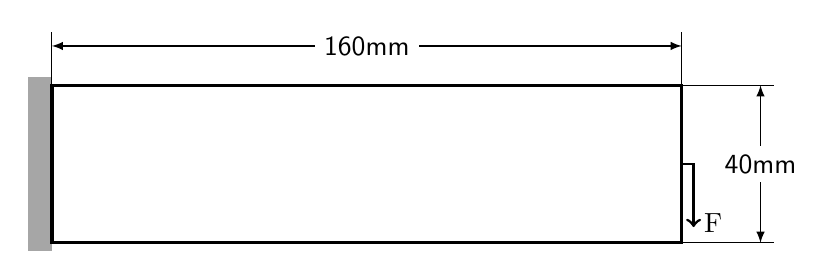
\begin{tikzpicture}
        \draw[fill,color=gray!70] (0,-0.1) rectangle (-0.3,2.1);
        \node [align=center, body,line width=1.2pt,minimum height=2cm,minimum width=8cm,anchor=south west] (body1) at (0,0) {};
        \draw (body1.south east) -- ++(1,0) coordinate (D1) -- +(5pt,0);
        \draw (body1.north east) -- ++(1,0) coordinate (D2) -- +(5pt,0);
        \draw [dimen] (D1) -- (D2) node {40mm};

        \draw (body1.north west) -- ++(0,0.5) coordinate (D1) -- +(0,5pt);
        \draw (body1.north east) -- ++(0,0.5) coordinate (D2) -- +(0,5pt);
        \draw [dimen] (D1) -- (D2) node {160mm};
        \draw[->,line width=1pt] (8,1) -- (8.15,1) -- (8.15,0.2);
        \node (arrowhead) at (8.4,0.25) {F};
    \end{tikzpicture} \newline
  }
  \caption{Cantilever beam problem before topology optimization.}
  \label{fig:CantBeam}
\end{figure}

\begin{figure}
  \centering
  \begin{subfigure}{0.7\textwidth}
    \resizebox{1\textwidth}{!}{
      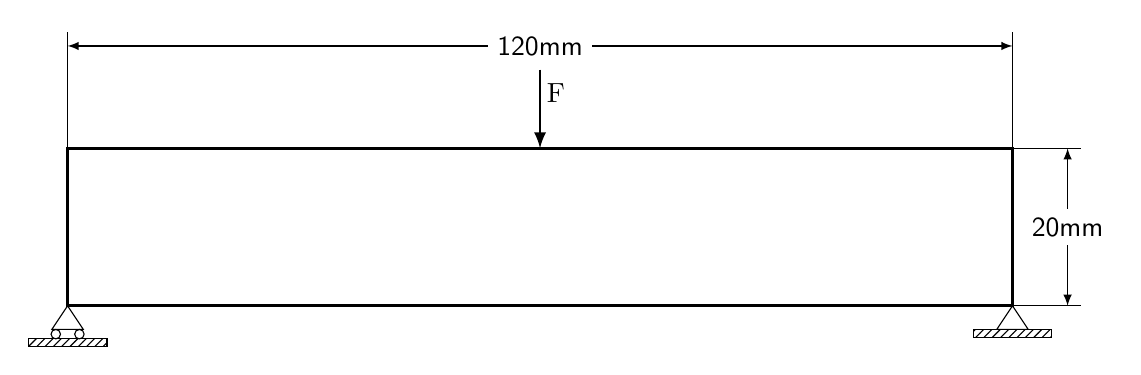
\begin{tikzpicture}[>=latex]
        \draw[line width=1.2pt] (-6,0) rectangle (6,2);
          \draw (6,0) -- ++(0.7,0) coordinate (D1) -- +(5pt,0);
          \draw (6,2) -- ++(0.7,0) coordinate (D2) -- +(5pt,0);
          \draw [dimen] (D1) -- (D2) node {20mm};
          \draw (-6,2) -- ++(0,1.3) coordinate (D3) -- +(0,5pt);
          \draw (6,2) -- ++(0,1.3) coordinate (D4) -- +(0,5pt);
          \draw [dimen] (D3) -- (D4) node {120mm};

        \draw (-6,0) -- (-6.2,-0.3) -- (-5.8,-0.3) -- cycle;
        \draw (-6.15,-0.36) circle (0.06);
        \draw (-5.85,-0.36) circle (0.06);
        \node [marked body,minimum height=0.1cm,minimum width=1cm,anchor=center] at (-6,-0.42-0.05) {};

        \draw (6,0) -- (6.2,-0.3) -- (5.8,-0.3) -- cycle;
        \node [marked body,minimum height=0.1cm,minimum width=1cm,anchor=center] at (6,-0.35) {};

        \draw[->,line width=1pt] (0,3) -- (0,2);
        \node (arrowhead) at (0.2,2.7) {F};
      \end{tikzpicture}
    }
    \caption{Full beam}
    \label{fig:FullMBB}
  \end{subfigure}
  \begin{subfigure}{0.4\textwidth}
    \hfill
    \resizebox{1\textwidth}{!}{
      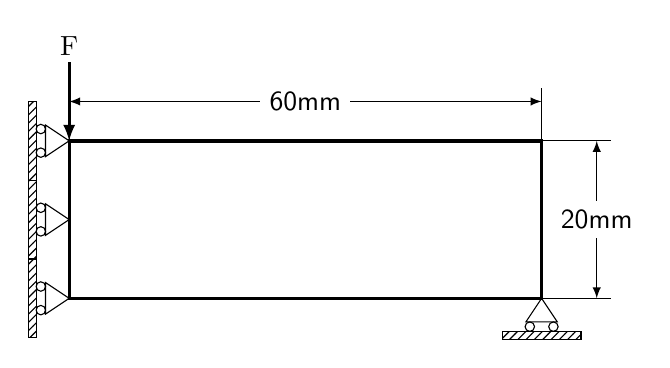
\begin{tikzpicture}[>=latex]
        \draw[line width=1.2pt] (0,0) rectangle (6,2);
        \draw (6,0) -- ++(0.7,0) coordinate (D1) -- +(5pt,0);
        \draw (6,2) -- ++(0.7,0) coordinate (D2) -- +(5pt,0);
        \draw [dimen] (D1) -- (D2) node {20mm};
        \draw (0,2) -- ++(0,0.5) coordinate (D3) -- +(0,5pt);
        \draw (6,2) -- ++(0,0.5) coordinate (D4) -- +(0,5pt);
        \draw [dimen] (D3) -- (D4) node {60mm};

        \draw (0,2) -- (-0.3,2.2) -- (-0.3,1.8) -- cycle;
        \draw (-0.36,2.15) circle (0.06);
        \draw (-0.36,1.85) circle (0.06);
        \node [marked body,minimum height=1cm,minimum width=0.1cm,anchor=center] at (-0.42-0.05,2) {};

        \draw (0,1) -- (-0.3,1.2) -- (-0.3,0.8) -- cycle;
        \draw (-0.36,1.15) circle (0.06);
        \draw (-0.36,0.85) circle (0.06);
        \node [marked body,minimum height=1cm,minimum width=0.1cm,anchor=center] at (-0.42-0.05,1) {};

        \draw (0,0) -- (-0.3,0.2) -- (-0.3,-0.2) -- cycle;
        \draw (-0.36,0.15) circle (0.06);
        \draw (-0.36,-0.15) circle (0.06);
        \node [marked body,minimum height=1cm,minimum width=0.1cm,anchor=center] at (-0.42-0.05,0) {};
        
        \draw (6,0) -- (6.2,-0.3) -- (5.8,-0.3) -- cycle;
        \draw (6.15,-0.36) circle (0.06);
        \draw (5.85,-0.36) circle (0.06);
        \node [marked body,minimum height=0.1cm,minimum width=1cm,anchor=center] at (6,-0.42-0.05) {};

        \draw[->,line width=1pt] (0,3) -- (0,2);
        \node (arrowhead) at (0,3.2) {F};
      \end{tikzpicture}
    }
    \caption{Half beam}
    \label{fig:HalfMBB}
  \end{subfigure}
  \caption{Messerschmitt-Bolkow-Blohm (MBB) beam problem}
  \label{fig:MBBBeam}
\end{figure}

\begin{figure}
  \centering
  \resizebox{0.5\textwidth}{!}{
    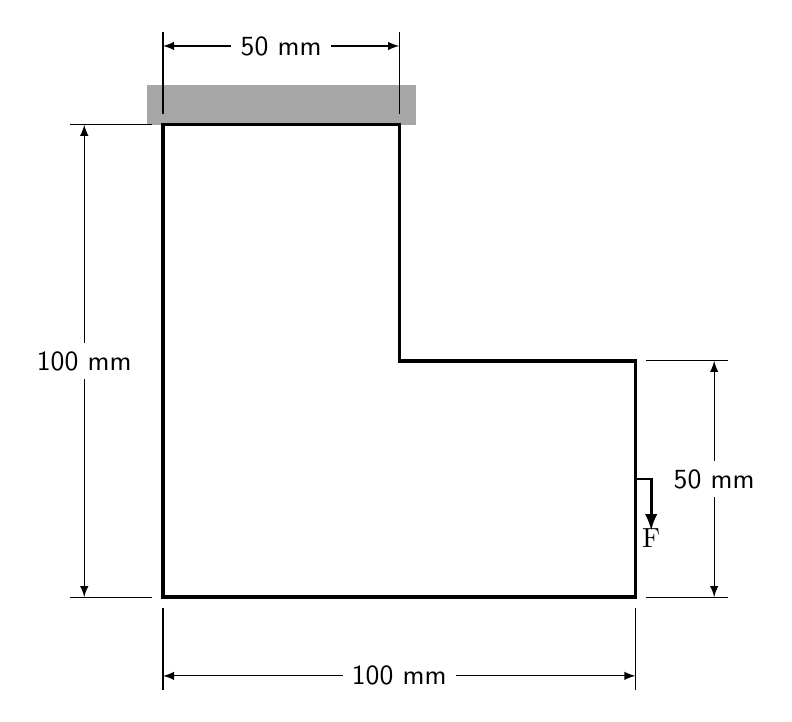
\begin{tikzpicture}[>=latex]
        \draw[fill,color=gray!70] (-0.2,2) rectangle (3.2,2.5);
        \draw[line width=1.2pt] (0, 2) node(nodeA){} -- (3, 2) node(nodeB){} -- (3, -1) -- (6, -1) node(nodeC){} -- (6, -4) node(nodeD){} -- (0, -4) node(nodeE){} -- cycle;
        
        \draw (nodeA) -- ++(0,1) coordinate (D1) -- +(0,5pt);
        \draw (nodeB) -- ++(0,1) coordinate (D2) -- +(0,5pt);
        \draw [dimen] (D1) -- (D2) node {50 mm};

        \draw (nodeA) -- ++(-1,0) coordinate (D1) -- +(-5pt,0);
        \draw (nodeE) -- ++(-1,0) coordinate (D2) -- +(-5pt,0);
        \draw [dimen] (D1) -- (D2) node {100 mm};

        \draw (nodeC) -- ++(1,0) coordinate (D1) -- +(5pt,0);
        \draw (nodeD) -- ++(1,0) coordinate (D2) -- +(5pt,0);
        \draw [dimen] (D1) -- (D2) node {50 mm};

        \draw (nodeE) -- ++(0,-1) coordinate (D1) -- +(0,-5pt);
        \draw (nodeD) -- ++(0,-1) coordinate (D2) -- +(0,-5pt);
        \draw [dimen] (D1) -- (D2) node {100 mm};

        \draw[->,line width=1pt] (6,-2.5) -- (6.2,-2.5) -- (6.2,-3.15);
        \node (arrowhead) at (6.2,-3.25) {F};
    \end{tikzpicture} \newline
  }
  \caption{L-shaped beam problem}
  \label{fig:LBeam}
\end{figure}
\end{comment}

\begin{figure}
  \centering
  \resizebox{0.7\textwidth}{!}{
    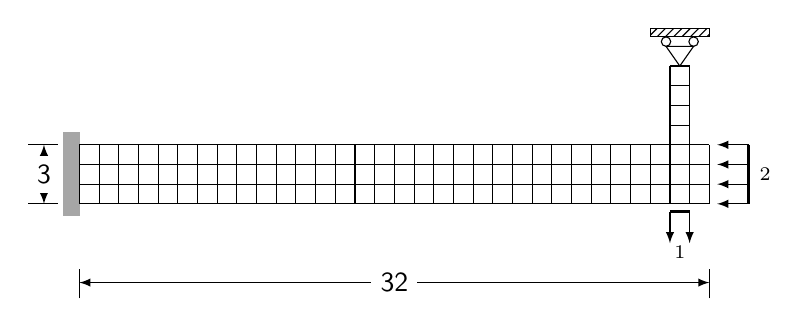
\begin{tikzpicture}[>=latex]
      \draw[fill,color=gray!70] (-0.2,-0.15) rectangle (0,0.9);
      \draw[step=0.25cm] (0,0) grid (8,0.75);
      \draw[step=0.25cm] (7.5,0.75) grid (7.75,1.75);
      \draw (7.5,0.75) -- (7.5,1.75);
      \draw (7.625,1.75) -- (7.8,2) -- (7.45,2) -- cycle;
      \draw (7.8,2.06) circle (0.06);
      \draw (7.45,2.06) circle (0.06);
      \node [marked body,minimum height=0.1cm,minimum width=0.75cm,anchor=center] at (7.625,2.18) {};

      \draw [->] (8.5,0) -- (8.1,0);
      \draw [->] (8.5,0.25) -- (8.1,0.25);
      \draw [->] (8.5,0.5) -- (8.1,0.5);
      \draw [->] (8.5,0.75) -- (8.1,0.75);
      \draw [line width=1.2pt] (8.5,0) -- (8.5,0.75) node[draw=none,fill=none,font=\scriptsize,midway,right] {2};
      
      \draw [->] (7.5,-0.1) -- (7.5,-0.5);
      \draw [->] (7.75,-0.1) -- (7.75,-0.5);
      \draw [line width=1.2pt] (7.5,-0.1) -- (7.75,-0.1) node[draw=none,fill=none,font=\scriptsize,midway,below,yshift=-0.3cm] {1};

      \draw (-0.65,0) -- ++(0.2,0) coordinate (D1) -- +(5pt,0);
      \draw (-0.65,0.75) -- ++(0.2,0) coordinate (D2) -- +(5pt,0);
      \draw [dimen] (D1) -- (D2) node {3};

      \draw (0,-1.2) -- ++(0,0.2) coordinate (D1) -- +(0,5pt);
      \draw (8,-1.2) -- ++(0,0.2) coordinate (D2) -- +(0,5pt);
      \draw [dimen] (D1) -- (D2) node {32};
    \end{tikzpicture}
  }
  \caption{Tie beam problem}
  \label{fig:TieBeam}
\end{figure}


\subsection{Genetic evolutionary structural optimization}

While ESO is an acronym for evolutionary structural optimization, it has no direct relationship with the Darwinian evolutionary algorithms (EAs), in fact ESO/BESO is a completely deterministic algorithm. Some specializations of the Darwinian EAs to topology optimization was also attempted in papers like \cite{Sandgren1990,Liu2008}. However, the so-called genetic ESO (GESO) method proposed by \cite{Liu2008} can also be viewed as a stochastic version of ESO/BESO since an unconventional definition of the solution population is used, where a single solution is treated as a population and every mesh element is a member of the population. This is different from the conventional meaning of a population in genetic algorithms (GAs), where a population must be made of many solutions each of which has an objective value and can be either feasible or not. The GA-like technique used by \cite{Liu2008} results in a stochastic re-ordering of the removal and addition of elements, compared to the deterministic BESO algorithm, which therefore makes it more like a binary stochastic gradient descent algorithm. Traditional EAs, e.g. GAs \citep{Sandgren1990}, and more generally zero-order optimization methods, e.g. pattern search \citep{Guirguis2016}, tried in literature fail to perform as well as SIMP and BESO since they require a prohibitively large number of function evaluations, more than 10s of thousands, even for toy problems, where each function evaluation can be an expensive FEA. Also the scale of problems required to be solved in practice can involve anywhere from 1000s to 100,000,000s of decision variables and zero-order methods are known for not scaling well when the number of decision variables is even in the 100s. On the other hand, SIMP and BESO tend to converge to good solutions in 100s of function evaluations at the very most, often in much less. Also huge scale problems with 10s of millions of decision variables were successfully solved in literature, e.g. \cite{Aage2015}, using these methods.

\subsection{Topology optimization problem classes}

A number of mechanical structure problems were studied and successfully solved in topology optimization literature where some of the objectives were: 

\begin{enumerate}[label=(\arabic*)]
  \item Compliance minimization \citep{Bendsoe1989}, 
  \item Material volume/cost minimization \citep{Payten1998,Bruggi2012}, 
  \item Maximum stress minimization \citep{Yang1996,Lian2017}, or 
  \item Minimum eigenvalue maximization \citep{Neves1995,Rahmatalla2003,Munk2017}. 
\end{enumerate}
Some of the constraints used were: 
\begin{enumerate}[label=(\arabic*)]
  \item Volume constraint \citep{Bendsoe1989}, 
  \item Maximum compliance constraint \citep{Bruggi2012,Collet2017}, 
  \item Maximum displacement constraint \citep{Huang2010a}, 
  \item Local/global stress constraints \citep{Payten1998,Amir2017}, 
  \item Fatigue constraints \citep{Oest2017,Collet2017}, and/or 
  \item Global stability/buckling/bifurcation constraints \citep{Kocvara2004,Browne2013,Deng2017}.
\end{enumerate}
Some of the mechanical systems studied were: 
\begin{enumerate}[label=(\arabic*)]
  \item Linear, elastic, quasi-static systems \citep{Bendsoe1989}, 
  \item Nonlinear, compliant mechanisms \citep{Sigmund1997}, 
  \item Nonlinear, elasto-plastic systems \citep{Maute1997,Amir2017}, or 
  \item Linear/nonlinear vibrating systems \citep{Zargham2016}. 
\end{enumerate}
And finally the loads handled were: 
\begin{enumerate}[label=(\arabic*)]
  \item Single or multiple \citep{Allaire2004}, 
  \item Design-independent or design-dependent \citep{Lee2012},
  \item Static or dynamic \citep{Zhang2016}, and 
  \item Deterministic or stochastic \citep{Zhang2016}. 
\end{enumerate}
Multiobjective problems combining multiple of the above objectives have also been scarcely considered \citep{Suresh2010,Sato2017a}. Many of the papers cited above have used either SIMP or BESO variants.

\begin{comment}
There are a number of problem domains, loading and boundary conditions commonly used for benchmarking and testing purposes. In this section, 3 common problem domains are summarized. 

a point load is applied on the center of the right end of a beam fixed on the other end as shown in Fig. \ref{fig:CantBeam}. A force $F = 1 \text{ N}$ was used, as well as a thickness of $1 \text{ mm}$ and a Young's modulus of $E = 1 \text{ MPa}$. This problem was solved by \cite{Huang2010a} to benchmark soft-kill BESO against CSIMP.


\begin{figure}[!htbp]
  \centering
  \resizebox{0.5\textwidth}{!}{
    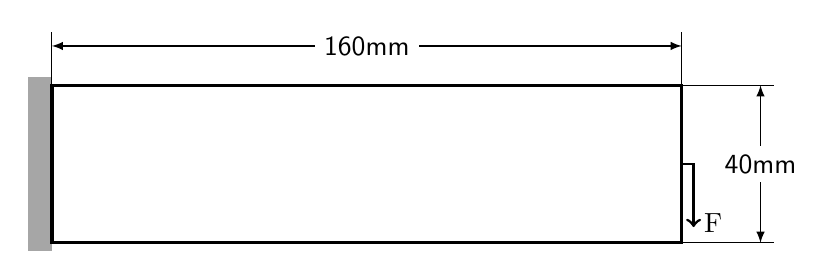
\begin{tikzpicture}
        \draw[fill,color=gray!70] (0,-0.1) rectangle (-0.3,2.1);
        \node [align=center, body,line width=1.2pt,minimum height=2cm,minimum width=8cm,anchor=south west] (body1) at (0,0) {};
        \draw (body1.south east) -- ++(1,0) coordinate (D1) -- +(5pt,0);
        \draw (body1.north east) -- ++(1,0) coordinate (D2) -- +(5pt,0);
        \draw [dimen] (D1) -- (D2) node {40mm};

        \draw (body1.north west) -- ++(0,0.5) coordinate (D1) -- +(0,5pt);
        \draw (body1.north east) -- ++(0,0.5) coordinate (D2) -- +(0,5pt);
        \draw [dimen] (D1) -- (D2) node {160mm};
        \draw[->,line width=1pt] (8,1) -- (8.15,1) -- (8.15,0.2);
        \node (arrowhead) at (8.4,0.25) {F};
    \end{tikzpicture} \newline
  }
  \caption{Cantilever beam problem before topology optimization.}
  \label{fig:CantBeam}
\end{figure}

\begin{figure}[!htbp]
  \centering
  \begin{subfigure}{0.7\textwidth}
    \resizebox{1\textwidth}{!}{
      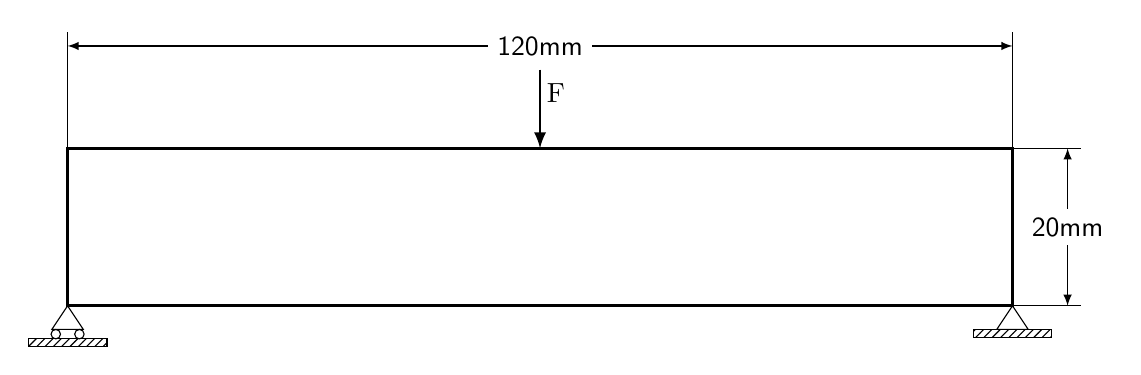
\begin{tikzpicture}[>=latex]
        \draw[line width=1.2pt] (-6,0) rectangle (6,2);
          \draw (6,0) -- ++(0.7,0) coordinate (D1) -- +(5pt,0);
          \draw (6,2) -- ++(0.7,0) coordinate (D2) -- +(5pt,0);
          \draw [dimen] (D1) -- (D2) node {20mm};
          \draw (-6,2) -- ++(0,1.3) coordinate (D3) -- +(0,5pt);
          \draw (6,2) -- ++(0,1.3) coordinate (D4) -- +(0,5pt);
          \draw [dimen] (D3) -- (D4) node {120mm};

        \draw (-6,0) -- (-6.2,-0.3) -- (-5.8,-0.3) -- cycle;
        \draw (-6.15,-0.36) circle (0.06);
        \draw (-5.85,-0.36) circle (0.06);
        \node [marked body,minimum height=0.1cm,minimum width=1cm,anchor=center] at (-6,-0.42-0.05) {};

        \draw (6,0) -- (6.2,-0.3) -- (5.8,-0.3) -- cycle;
        \node [marked body,minimum height=0.1cm,minimum width=1cm,anchor=center] at (6,-0.35) {};

        \draw[->,line width=1pt] (0,3) -- (0,2);
        \node (arrowhead) at (0.2,2.7) {F};
      \end{tikzpicture}
    }
    \caption{Full beam}
    \label{fig:FullMBB}
  \end{subfigure}
  \begin{subfigure}{0.4\textwidth}
    \hfill
    \resizebox{1\textwidth}{!}{
      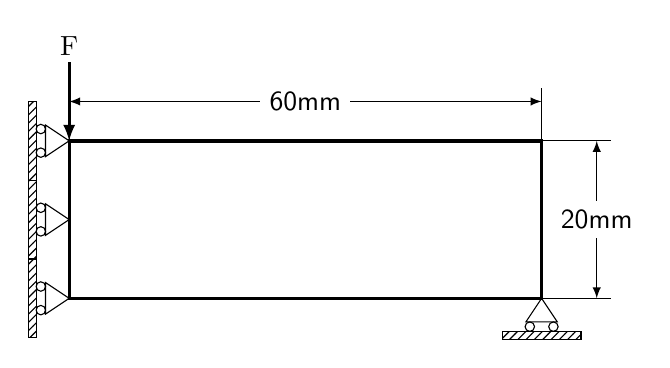
\begin{tikzpicture}[>=latex]
        \draw[line width=1.2pt] (0,0) rectangle (6,2);
        \draw (6,0) -- ++(0.7,0) coordinate (D1) -- +(5pt,0);
        \draw (6,2) -- ++(0.7,0) coordinate (D2) -- +(5pt,0);
        \draw [dimen] (D1) -- (D2) node {20mm};
        \draw (0,2) -- ++(0,0.5) coordinate (D3) -- +(0,5pt);
        \draw (6,2) -- ++(0,0.5) coordinate (D4) -- +(0,5pt);
        \draw [dimen] (D3) -- (D4) node {60mm};

        \draw (0,2) -- (-0.3,2.2) -- (-0.3,1.8) -- cycle;
        \draw (-0.36,2.15) circle (0.06);
        \draw (-0.36,1.85) circle (0.06);
        \node [marked body,minimum height=1cm,minimum width=0.1cm,anchor=center] at (-0.42-0.05,2) {};

        \draw (0,1) -- (-0.3,1.2) -- (-0.3,0.8) -- cycle;
        \draw (-0.36,1.15) circle (0.06);
        \draw (-0.36,0.85) circle (0.06);
        \node [marked body,minimum height=1cm,minimum width=0.1cm,anchor=center] at (-0.42-0.05,1) {};

        \draw (0,0) -- (-0.3,0.2) -- (-0.3,-0.2) -- cycle;
        \draw (-0.36,0.15) circle (0.06);
        \draw (-0.36,-0.15) circle (0.06);
        \node [marked body,minimum height=1cm,minimum width=0.1cm,anchor=center] at (-0.42-0.05,0) {};
        
        \draw (6,0) -- (6.2,-0.3) -- (5.8,-0.3) -- cycle;
        \draw (6.15,-0.36) circle (0.06);
        \draw (5.85,-0.36) circle (0.06);
        \node [marked body,minimum height=0.1cm,minimum width=1cm,anchor=center] at (6,-0.42-0.05) {};

        \draw[->,line width=1pt] (0,3) -- (0,2);
        \node (arrowhead) at (0,3.2) {F};
      \end{tikzpicture}
    }
    \caption{Half beam}
    \label{fig:HalfMBB}
  \end{subfigure}
  \caption{Messerschmitt-Bolkow-Blohm (MBB) beam problem}
  \label{fig:MBBBeam}
\end{figure}

\begin{figure}[!htbp]
  \centering
  \resizebox{0.5\textwidth}{!}{
    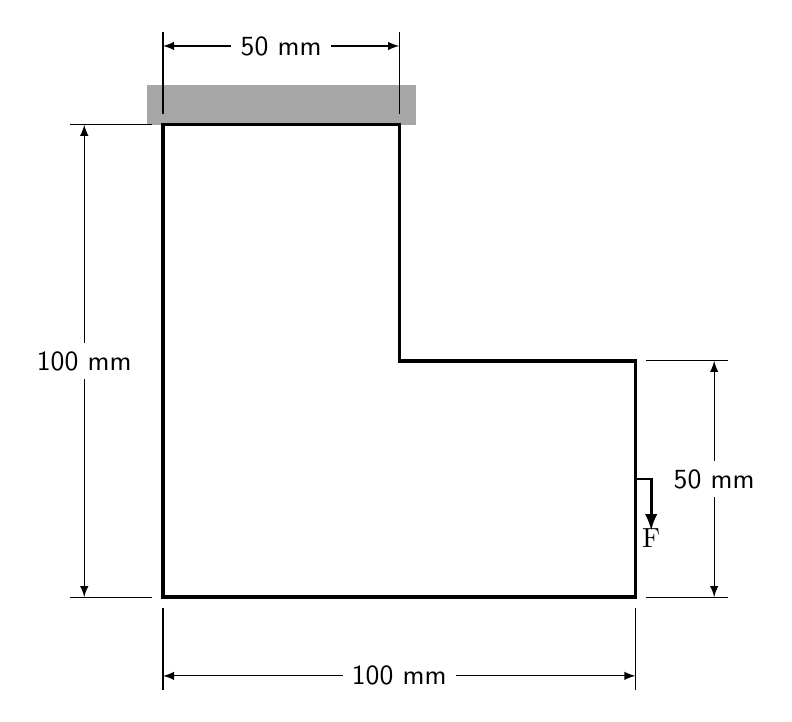
\begin{tikzpicture}[>=latex]
        \draw[fill,color=gray!70] (-0.2,2) rectangle (3.2,2.5);
        \draw[line width=1.2pt] (0, 2) node(nodeA){} -- (3, 2) node(nodeB){} -- (3, -1) -- (6, -1) node(nodeC){} -- (6, -4) node(nodeD){} -- (0, -4) node(nodeE){} -- cycle;
        
        \draw (nodeA) -- ++(0,1) coordinate (D1) -- +(0,5pt);
        \draw (nodeB) -- ++(0,1) coordinate (D2) -- +(0,5pt);
        \draw [dimen] (D1) -- (D2) node {50 mm};

        \draw (nodeA) -- ++(-1,0) coordinate (D1) -- +(-5pt,0);
        \draw (nodeE) -- ++(-1,0) coordinate (D2) -- +(-5pt,0);
        \draw [dimen] (D1) -- (D2) node {100 mm};

        \draw (nodeC) -- ++(1,0) coordinate (D1) -- +(5pt,0);
        \draw (nodeD) -- ++(1,0) coordinate (D2) -- +(5pt,0);
        \draw [dimen] (D1) -- (D2) node {50 mm};

        \draw (nodeE) -- ++(0,-1) coordinate (D1) -- +(0,-5pt);
        \draw (nodeD) -- ++(0,-1) coordinate (D2) -- +(0,-5pt);
        \draw [dimen] (D1) -- (D2) node {100 mm};

        \draw[->,line width=1pt] (6,-2.5) -- (6.2,-2.5) -- (6.2,-3.15);
        \node (arrowhead) at (6.2,-3.25) {F};
    \end{tikzpicture} \newline
  }
  \caption{L-shaped beam problem}
  \label{fig:LBeam}
\end{figure}

\end{comment}

\newpage
\section{Nonlinear programming}

Part of the SIMP algorithm is solving an NLP using a constrained mathematical optimization algorithm. Zero-order algorithms don't scale too well so they are typically not used for topology optimization. Second order algorithms requiring Hessians are typically too computationally prohibitive because the Hessian with respect to per-element decision variables will typically be a huge dense matrix. Therefore, first order algorithms are by far the most commonly used class of algorithms in topology optimization. There are 2 notable algorithms that were developed specifically for SIMP:
\begin{enumerate}
    \item The method of moving asymptotes (MMA) \citep{Svanberg1987} and its globally convergent extension \citep{Svanberg2002}.
    \item The convex linearization method (CONLIN) \citep{Fleury1989}
\end{enumerate}
Other algorithms that have been used in literature \citep{Rojas-Labanda2015,Pereira2004,tarek2021robust} include:
\begin{enumerate}
    \item The primal-dual interior point optimizer (IPOPT) \citep{Wachter2006}, with the limited memory Broyden, Fletcher, Goldfarb, and Shann (l-BFGS) approximation of the inverse Lagrangian Hessian \citep{Nocedal2006}
    \item The first order augmented Lagrangian (AugLag) algorithm \citep{Bertsekas1996}.
\end{enumerate}

In this section, the original MMA, IPOPT and AugLag will be explained further because they are used in the thesis. Notably, MMA cannot handle equality constraints directly, only inequality constraints, while IPOPT and AugLag handle both equality and inequality constraints. MMA, IPOPT and AugLag are all local optimization algorithms that seek to find a so-called KKT point, which under certain assumptions is a local optimum solution.

In this section, the terms \textit{linear} and \textit{affine} will be used inter-changeably in the context of classifying a function/constraint as either a linear/affine or a nonlinear function/constraint. Even though there is a distinction between the 2 terms, optimization literature commonly uses these 2 terms inter-changeably for the same purpose.

\subsection{Formulations}

There are generally a number of ways to formulate the same optimization or decision problem using mathematical functions and decision variables. For instance, consider the following inequality constrained optimization problem:
\begin{mini}|l|[3]
  {\bm{x}}{f_0(\bm{x})}{\label{form:I}}{}
  \addConstraint {f_i(\bm{x})}{\leq 0}{\quad \forall i = 1..I}
  \addConstraint {l_j \leq x_j \leq u_j}{}{\quad \forall j = 1..V}
\end{mini}
where $I$ is the number of constraints, $V$ is the number of decision variables, $f_i$ is a potentially nonlinear scalar-valued function of $\bm{x}$ and $\bm{l}$ and $\bm{u}$ are finite vectors of lower and upper bounds on the decision vector $\bm{x}$ respectively. Two formulations are considered equivalent for optimization purposes if every optimal solution of one formulation maps to an optimal solution in the other formulation. In the following sub-sections, 2 relevant re-formulation tricks will be presented. For more re-formulation techniques, the readers are referred to the excellent online book titled: "MOSEK Modeling Cookbook" by MOSEK ApS \citep{mosekcookbook}.

\subsubsection{A linear objective is all you need}

For instance, consider the alternative formulation:
\begin{mini}|l|[3]
  {\bm{x}, c}{c \label{form:II}}{}{}
  \addConstraint {f_0(\bm{x})}{\leq c}{}
  \addConstraint {f_i(\bm{x})}{\leq 0}{\quad \forall i = 1..I}
  \addConstraint {l_j \leq x_j \leq u_j}{}{\quad \forall j = 1..V}
\end{mini}
where we added a new decision variable $c$ and a new constraint $f_0(\bm{x}) \leq c$ to the previous formulation and changed the objective to minimizing $c$ which is a linear function of the decision variables.

It is clear that if $\bm{x}^*$ is an optimal solution of formulation \ref{form:I}, then $(\bm{x}, c) = (\bm{x}^*, f_0(\bm{x}^*))$ is optimal in formulation \ref{form:II}. This is because $f_0(\bm{x}^*)$ is the lowest value $f_0(\bm{x})$ can take for any feasible $\bm{x}$ according to the remaining inequality constraints, and $c = f_0(\bm{x}^*)$ is the lowest value the objective $c$ can take without violating the constraint on $c$.

Conversely, if $(\bm{x}^*, c^*)$ is an optimal solution of formulation \ref{form:II}, $\bm{x}^*$ must be optimal in formulation \ref{form:I}. Since $c$ shows up in only one constraint:
\begin{align}
    f_0(\bm{x}) \leq c
\end{align}
in formulation \ref{form:II}, for $(\bm{x}^*, c^*)$ to be optimal, $c^*$ must be equal to $f_0(\bm{x}^*)$. And since this is lowest value $c$ can take, it must be the lowest value $f_0(\bm{x})$ can take without violating any of the other constraints on $\bm{x}$, which in turn makes $\bm{x}^*$ an optimal solution to formulation \ref{form:I}. This completes the proof.

\subsubsection{Slack variables}

Another common formulation transformation is changing all the inequality constraints to equality constraints except the variable bounds. This can be done by introducing additional slack variables. Let $\bm{s}$ be a vector of so-called slack variables with length $I$, where $s_i$ is the $i^{th}$ element of the vector associated with constraint $i$ for $i \in 1..I$. Formulation \ref{form:I} can be re-written as:
\begin{mini}|l|[3]
  {\bm{x}, \bm{s}}{f_0(\bm{x})}{\label{form:III}}{}
  \addConstraint {f_i(\bm{x}) + s_i}{= 0}{\quad \forall i = 1..I}
  \addConstraint {l_j \leq x_j \leq u_j}{}{\quad \forall j = 1..V}
  \addConstraint {s_i \geq 0}{}{\quad \forall i = 1..I}
\end{mini}

Since $\bm{s}$ doesn't show up in the objective, in order to prove that formulations \ref{form:I} and \ref{form:III} are equivalent for optimization purposes, it suffices to show that every feasible solution $\bm{x}$ to formulation \ref{form:I} can be mapped a feasible solution $(\bm{x}, \bm{s})$ in formulation \ref{form:III} and vice versa.

It is simple to show that if $\bm{x}$ is a feasible solution in formulation \ref{form:I}, that $(\bm{x}, \bm{s})$ where $\bm{s}: s_i = -f_i(\bm{x})\, \forall i \in 1..I$ is a feasible solution in formulation \ref{form:III}. This is because for $\bm{x}$ to be feasible in formulation \ref{form:I}, $f_i(\bm{x})$ must be non-positive for all $i$ which makes $s_i$ non-negative. Conversely, if $(\bm{x}, \bm{s})$ is a feasible solution to formulation \ref{form:III}, $\bm{x}$ is clearly feasible in formulation \ref{form:I} because $s_i$ will be non-negative which implies that $f_i(\bm{x}) \leq 0$ for all $i$. This completes the proof.

\subsubsection{Equality constraints and empty interiors}

While the following equality constraint:
\begin{align}
  f(\bm{x}) = 0
\end{align}
is in theory equivalent to the following 2 inequality constraints:
\begin{align}
  0 \leq f(\bm{x}) \leq 0
\end{align}
this transformation does not change the shape or nature of the feasible domain. Not all NLP algorithms that can handle inequality constraints can also handle problems with 2 inequality constraints derived from an equality constraint like this. For instance, the convergence proof of the globally convergent MMA algorithm \citep{Svanberg2002} assumes that the feasible domain must have a non-empty interior. Equality constraints introduce an "empty interior". A domain $D \subseteq \mathbb{R}^V$ is said to have a non-empty interior if $\exists (\bm{x}_c \in D, r > 0)$ such that $\bm{x}_c + \bm{u} \in D$ for all $\bm{u}$ in $\{\bm{u} : \bm{u} \in \mathbb{R}^V \wedge ||\bm{u}||_2 \leq r\}$. Since equality constraints change the feasible domain to a lower dimensional manifold embedded in $\mathbb{R}^V$, there exist no such $(\bm{x}_c, r)$ in equality constrained problems. Therefore, the MMA algorithm will fail if the interior of the feasible domain is empty.

Linear equality constraints are generally an exception though. While technically still introducing an empty interior, most NLP algorithms can either natively handle linear equality constraints or the linear equality constrained NLP can be re-parameterized such that the interior of the feasible domain is no longer empty. IPOPT and AugLag can handle linear and even nonlinear equality constraints natively. Sequential quadratic programming (SQP) methods \citep{Boyd2009} can only handle linear equality constraints natively whereas nonlinear ones must get locally approximated by linear ones in an iterative process. MMA however doesn't handle either linear or nonlinear equality constraints natively. But it can be made to support linear ones with a simple nullspace re-parameterization trick.

Let the following be the linear equality constrained NLP with a nonlinear objective and inequality constraints:
\begin{mini}|l|[3]
  {\bm{x}}{f_0(\bm{x})}{\label{form:IV}}{}
  \addConstraint {f_i(\bm{x})}{\leq 0}{\quad \forall i = 1..I}
  \addConstraint {l_j \leq x_j \leq u_j}{}{\quad \forall j = 1..V}
  \addConstraint {\bm{A} \bm{x}}{= b}{}
\end{mini}
where $\bm{A}$ is a constant matrix of size $(M \times V)$ and $\bm{b}$ is a constant vector. Let $\bm{x}_0$ be an arbitrary point that satisfies the $\bm{A} \bm{x} = \bm{b}$ constraint, e.g. $\bm{x}_0 = \bm{A}^{+} \bm{b}$ where $\bm{A}^{+}$ is the Moore-Penrose pseudoinverse of $\bm{A}$ \citep{Golub1996}. Let $\bm{N}$ be the nullspace matrix of $\bm{A}$ such that $\bm{A} \times \bm{N} = \bm{0}$, where $\bm{N}$ is of size $V \times U$. Every feasible solution $\bm{x}$ to the constraints $\bm{A} \bm{x} = \bm{b}$ can now be written as:
\begin{align}
    \bm{x} = \bm{x}_0 + \bm{N} \bm{y}
\end{align}
for some $\bm{y} \in \mathbb{R}^U$, where $U < V$. Substituting for $\bm{x}$ in formulation \ref{form:IV}, we get:
\begin{mini}|l|[3]
  {\bm{y}}{f_0(\bm{x}_0 + \bm{N} \bm{y})}{\label{form:V}}{}
  \addConstraint {f_i(\bm{x}_0 + \bm{N} \bm{y})}{\leq 0}{\quad \forall i = 1..I}
  \addConstraint {\bm{l} \leq \bm{x}_0 + \bm{N} \bm{y} \leq \bm{u}}{}{}
\end{mini}
The re-parameterization essentially limits the feasible domain to the nullspace of the linear constraints since the "interior" is non-empty once we limit ourselves to the nullspace. A similar re-parameterization trick can also be used for some nonlinear manifolds, e.g. optimization on the surface of a hyper-sphere.

Beside the iterative linear approximation of nonlinear equality constraints, MMA can also be made to approximately support nonlinear equality constraints by relaxing it as follows:
\begin{align}
  -\epsilon \leq f(\bm{x}) \leq \epsilon
\end{align}
where $\epsilon > 0$ which creates a non-empty interior.

\subsection{Regularity conditions}

There are a number of optimization algorithms that can solve a general NLP without assuming convexity. Most NLP algorithms tend to converge to a locally optimal solution without global optimality guarantees and this suffices in many applications. For simplicity, assume all the inequality constraints have been converted to equality constraints using slack variables. Let the NLP with equality constraints be:
\begin{mini!}|l|[3]
  {\bm{x}}{f(\bm{x})}{}{}
  \addConstraint {\quad \bm{c}(\bm{x}) = \bm{0}}{}
  \addConstraint {\quad \bm{l} \leq \bm{x} \leq \bm{u}}{}
\end{mini!}
where $\bm{c}(\bm{x})$ is of length $E$. Additionally, let $f$ and $\bm{c}$ be continuous and twice differentiable functions.

A point $\bm{x}$ is called a regular point if it satisfies one of the so-called constraint qualification conditions. Three common constraint qualifications for NLPs are:
\begin{enumerate}
    \item Linear constraint qualification (LCQ): $\bm{c}(\bm{x})$ is an affine function.
    \item Linear independence constraint qualification (LICQ): the rows of $\nabla \bm{c}(\bm{x})$ and the gradients of the active (i.e. satisfied at equality) bound constraints are linearly independent at $\bm{x}$.
    \item Mangasarian-Fromovitz constraint qualification (MFCQ): the rows of $\nabla \bm{c}(\bm{x})$ are linearly independent at $\bm{x}$ and there exists a direction vector $\bm{d} \in \mathbb{R}^V$ where $d_i > 0$ if $x_i = l_i$, $d_i < 0$ if $x_i = u_i$, and $\nabla \bm{c}(\bm{x})^T \bm{d} = \bm{0}$.
\end{enumerate}

Alternatively, if the problem is convex and the nonlinear inequality constraints are not converted to equality constraints, every feasible point is regular if $\exists \bm{x}$ such that all the inequality constraints are satisfied but not active (i.e. satisfied at a strict inequality) and all the linear equality constraints are satisfied. This condition is known as Slater's condition \citep{Boyd2009}.

\subsection{Sufficient optimality conditions for regular points}

Let:
\begin{align}
  L(\bm{x}, \bm{\lambda}, \bm{z}_+, \bm{z}_-) = f(\bm{x}) + \bm{c}(\bm{x})^T \bm{\lambda} + (\bm{x} - \bm{u})^T \bm{z}_+  - (\bm{x} - \bm{l})^T \bm{z}_-
\end{align}
where $\bm{\lambda} \in \mathbb{R}^E$ is the vector of Lagrangian multipliers of the nonlinear constraints, $\bm{z}_- \in \mathbb{R}^V_+$ is the vector of Lagrangian multipliers of the $\geq$ bound constraints, and $\bm{z}_+ \in \mathbb{R}^V_+$ is the vector of Lagrangian multipliers of the $\leq$ bound constraints.

If $\bm{x}$ is regular and is a local optimum of the NLP, then $\exists (\bm{\lambda}, \bm{z}_+, \bm{z}_-)$ such that:
\begin{align}
  \nabla_{\bm{x}} L(\bm{x}, \bm{\lambda}, \bm{z}_+, \bm{z}_-) = \bm{0} \label{eqn:stationarity} \\
  \bm{c}(\bm{x}) = 0  \label{eqn:primal_feasible_1} \\
  \bm{l} \leq \bm{x} \leq \bm{u}  \label{eqn:primal_feasible_2}  \\
  \bm{z}_+ \geq \bm{0}  \label{eqn:dual_feasible_1}  \\
  \bm{z}_- \geq \bm{0} \label{eqn:dual_feasible_2} \\
  (\bm{x} - \bm{u})^T \bm{z}_+ = 0 \label{eqn:complementarity_1} \\
  (\bm{x} - \bm{l})^T \bm{z}_- = 0 \label{eqn:complementarity_2} \\
  \nabla \bm{c}(\bm{x})^T \nabla_{\bm{x}\bm{x}}^2 L(\bm{x}, \bm{\lambda}, \bm{z}_+, \bm{z}_-) \nabla \bm{c}(\bm{x}) \succcurlyeq \bm{0} \label{eqn:second_order}
\end{align}
These conditions are known as the KKT sufficient conditions for optimality and $\bm{x}$ would be called a KKT point \citep{Boyd2009}. Condition \ref{eqn:stationarity} is known as the stationarity condition which generalizes the 0 gradient condition for unconstrained NLPs. Conditions \ref{eqn:primal_feasible_1} and \ref{eqn:primal_feasible_2} are known as primal feasibility conditions. Conditions \ref{eqn:dual_feasible_1} and \ref{eqn:dual_feasible_2} are known as dual feasibility conditions. Finally, condition \ref{eqn:second_order} is known as the second order KKT optimality condition which generalizes the second order optimality condition for unconstrained NLPs, where $\bm{A} \succcurlyeq \bm{0}$ when $\bm{A}$ is a matrix means that $\bm{A}$ must be positive semi-definite.

Note that not every local optimal solution to the NLP must be a regular point or by consequence a KKT point for that matter. Therefore, these conditions are not necessary conditions for optimality for general NLPs. However for convex problems, if Slater's condition is satisfied, these conditions are both necessary and sufficient and the local/global optimum is guaranteed to be a regular and a KKT point \citep{Boyd2009}. All the optimization algorithms presented next seek to find a locally optimal KKT point.

\subsection{Method of moving asymptotes}

  Consider the following inequality constrained optimization problem:
  \begin{mini}|l|[3]
    {\bm{x}}{f_0(\bm{x})}{\label{form:I}}{}
    \addConstraint {f_i(\bm{x})}{\leq 0}{\quad \forall i = 1..I}
    \addConstraint {l_j \leq x_j \leq u_j}{}{\quad \forall j = 1..V}
  \end{mini}
  where $I$ is the number of inequality constraints, $V$ is the number of decision variables, $f_i$ is a potentially nonlinear scalar-valued function of $\bm{x}$ and $\bm{l}$ and $\bm{u}$ are finite vectors of lower and upper bounds on the decision vector $\bm{x}$ respectively.

  The first MMA algorithm proposed by \cite{Svanberg1987} relied on a separable convex approximation of the objective and constraint functions. A function $f(\bm{x})$ is linearly approximated with respect to either $t_{l,j}$ or $t_{u,j}$, where:
  \begin{align}
      t_{l,j} = t_l(x_j; L_j) = \frac{1}{x_j - L_j} \\
      t_{u,j} = t_u(x_j; U_j) = \frac{1}{U_j - x_j}
  \end{align}
  for all $j \in 1..V$ for some constants $L_j$ and $U_j$, where $l_j \leq L_j < U_j \leq u_j$, and $L_j$ and $U_j$ are known as the asymptotes of the approximation. The choice of which function, $t_{l,j}$ or $t_{u,j}$, to approximate $f$ with respect to, for each variable $x_j$, depends on the sign of the partial derivative $\frac{\partial f}{\partial x_j}$ such that the approximation is convex.

  More specifically, let the MMA approximation of $f(\bm{x})$ around $\bar{\bm{x}}$ be:
  \begin{align}
    \bar{f}(\bm{x}; \bar{\bm{x}}) = f(\bar{\bm{x}}) + \Sigma_j \bar{f}_j(x_j; \bar{\bm{x}})
  \end{align}
  Let $\bar{f}_j(x_j; \bar{\bm{x}})$ be:
  \begin{align}
    \bar{f}_j(x_j; \bar{\bm{x}}) & = \begin{cases}
      \Bigl( t_l(x_j; L_j) - t_l(\bar{x}_j; L_j) \Bigr) \frac{\partial f}{\partial t_{l,j}}(\bar{\bm{x}}), & \frac{\partial f}{\partial x_j}(\bar{\bm{x}}) < 0 \\
      \Bigl( t_u(x_j; U_j) - t_u(\bar{x}_j; U_j) \Bigr) \frac{\partial f}{\partial t_{u,j}}(\bar{\bm{x}}), & \frac{\partial f}{\partial x_j}(\bar{\bm{x}}) \geq 0
    \end{cases}
  \end{align}
  where $\bar{x}_j$ is the $j^{th}$ element of $\bar{\bm{x}}$ and $\frac{\partial f}{\partial t_{l,j}}$ and $\frac{\partial f}{\partial t_{u,j}}$ are:
  \begin{align}
    & \frac{\partial f}{\partial t_{l,j}} = \frac{\partial f}{\partial x_j} / \frac{d t_{l,j}}{d x_j} = - (x_j - L_j)^2 \frac{\partial f}{\partial x_j} \\
    & \frac{\partial f}{\partial t_{u,j}} = \frac{\partial f}{\partial x_j} / \frac{d t_{u,j}}{d x_j} = (U_j - x_j)^2 \frac{\partial f}{\partial x_j}
  \end{align}
  $\bar{f}_j(x_j; \bar{\bm{x}})$ can therefore be written as:
  \begin{align}
    \bar{f}_j(x_j; \bar{\bm{x}}) & = \begin{cases}
      -\Bigl( t_l(x_j; L_j) - t_l(\bar{x}_j; L_j) \Bigr) (\bar{x}_j - L_j)^2 \frac{\partial f}{\partial x_j}(\bar{\bm{x}}), & \frac{\partial f}{\partial x_j}(\bar{\bm{x}}) < 0 \\
      \Bigl( t_u(x_j; U_j) - t_u(\bar{x}_j; U_j) \Bigr) (U_j - \bar{x}_j)^2 \frac{\partial f}{\partial x_j}(\bar{\bm{x}}), & \frac{\partial f}{\partial x_j}(\bar{\bm{x}}) \geq 0
    \end{cases}
  \end{align}  

  The signs of the gradient and Hessian of $\bar{f}(\bm{x}; \bar{\bm{x}})$ therefore depend mostly on $t_l(x_j; L_j)$ and $t_u(x_j; U_j)$. Since the approximation is separable in $\bm{x}$, the Hessian of $\bar{f}(\bm{x}; \bar{\bm{x}})$ wrt $\bm{x}$ is a diagonal matrix where the $j^{th}$ diagonal element is:
  \begin{align}
    \frac{\partial^2 \bar{f}}{\partial x_j^2} = \begin{cases}
      -\frac{d^2 t_{l,j}}{d x_j^2} (\bar{x}_j - L_j)^2 \frac{\partial f}{\partial x_j}(\bar{\bm{x}}), & \frac{\partial f}{\partial x_j}(\bar{\bm{x}}) < 0 \\
      \frac{d^2 t_{u,j}}{d x_j^2} (U_j - \bar{x}_j)^2 \frac{\partial f}{\partial x_j}(\bar{\bm{x}}), & \frac{\partial f}{\partial x_j}(\bar{\bm{x}}) \geq 0
    \end{cases}
  \end{align}
  Since $\frac{d^2 t_{l,j}}{d x_j^2}$ and $\frac{d^2 t_{u,j}}{d x_j^2}$ are both positive for all $x_j$, it is clear that the MMA approximation is always going to be convex.

  In each iteration of the MMA algorithm, convex approximations of the objective and all the constraint functions are formed around the current solution and the approximate problem is solved to optimality while restricting the decision variables to be between the asymptotes $\bm{L}$ and $\bm{U}$ instead of the original bounds $\bm{l}$ and $\bm{u}$. This is similar to the trust region approach. Let the restricted convex approximation of the original nonlinear program be:
  \begin{mini*}|l|[3]
    {\bm{x}}{\bar{f}_0(\bm{x}; \bar{\bm{x}})}{}{}
    \addConstraint {\bar{f}_i(\bm{x}; \bar{\bm{x}})}{\leq 0}{\quad \forall i = 1..I}
    \addConstraint {\alpha_j \leq x_j \leq \beta_j}{}{\quad \forall j = 1..V}
  \end{mini*}
  where each decision variable $x_j$ is restricted to be between $\alpha_j = max(l_j, L_j)$ and $\beta_j = min(u_j, U_j)$ and $\bar{f}_i(\bm{x}; \bar{\bm{x}})$ is the MMA approximation of $f_i(\bm{x})$ around $\bar{\bm{x}}$. In order to form the approximation above, the gradient of the objective and the full Jacobian of the constraint functions need to be computed first. This typically limits the MMA algorithm's scalability in handling many constraints where the full Jacobian can be expensive to form, e.g. in stress-constrained topology optimization. However if only a few constraints exist, the MMA algorithm is usually quite robust when starting from a feasible solution. Most importantly is that once the approximate problem is formed, no more calls to the objective or constraint kernels are required by the primal-dual algorithm to solve the approximate problem to optimality.

  Once the approximation is formed, the separable nature of the MMA convex approximation then allows the approximate nonlinear program to be solved to optimality using an efficient primal-dual Lagrangian optimization algorithm \citep{Svanberg1987}. The dual of the convex approximation problem above is the following lower bound constrained nested optimization problem:
  \begin{maxi*}|l|[3]
    {\bm{\bm{\lambda} \geq \bm{0}}}{\min_{\bm{l} \leq \bm{x} \leq \bm{u}} \mathcal{L}(\bm{x}, \bm{\lambda}) = r_0 + \sum_{j=1}^V \mathcal{L}_j}{}{}
  \end{maxi*}
  where
  \begin{align}
    \mathcal{L}_j(x_j; \bm{\lambda}) & = \frac{p_{0,j} + \sum_i \lambda_i p_{i,j}}{U_j - x_j} + \frac{q_{0,j} + \sum_i \lambda_i q_{i,j}}{x_j - L_j} \\
    r_0 & = f_0(\bar{\bm{x}}) - \sum_{j=1}^V \frac{p_{0,j}}{U_j - \bar{x}_j} + \frac{q_{0,j}}{\bar{x}_j - L_j} \\
    p_{i,j} & = \begin{cases}
      (U_j - \bar{x}_j)^2 \frac{\partial f_i}{\partial x_j}(\bar{\bm{x}}) & \frac{\partial f_i}{\partial x_j}(\bar{\bm{x}}) > 0 \\
      0 & \frac{\partial f_i}{\partial x_j}(\bar{\bm{x}}) \leq 0
    \end{cases} \\
    q_{i,j} & = \begin{cases}
      0 & \frac{\partial f_i}{\partial x_j}(\bar{\bm{x}}) \geq 0 \\
      -(\bar{x}_j - L_j)^2 \frac{\partial f_i}{\partial x_j}(\bar{\bm{x}}) & \frac{\partial f_i}{\partial x_j}(\bar{\bm{x}}) < 0
  \end{cases}
  \end{align}
  The primal optimal solution $\bm{x}^*$ of the convex approximation has an analytic form as a function of the dual solution $\bm{\lambda}$:
  \begin{align}
    x^*_j(\bm{\lambda}) = \begin{cases}
      \alpha_j & \frac{\partial \mathcal{L}_j}{\partial x_j}(\alpha_j; \bm{\lambda}) \geq 0 \\
      \beta_j & \frac{\partial \mathcal{L}_j}{\partial x_j}(\beta_j; \bm{\lambda}) \leq 0 \\
      \frac{(p_{0,j} + \sum_i \lambda_i p_{i,j})^{1/2} L_j + (q_{0,j} + \sum_i \lambda_i q_{i,j})^{1/2} U_j}{(p_{0,j} + \sum_i \lambda_i p_{i,j})^{1/2} + (q_{0,j} + \sum_i \lambda_i q_{i,j})^{1/2}} & otherwise
    \end{cases}
  \end{align}

  Since the optimization of the approximate nonlinear program requires no calls to the objective or constraint kernels, its performance is independent of the computational complexity of computing the objective value, its gradient, the constraint values and their Jacobian.
  
  One of the biggest numerical challenges in topology optimization is that the scale of the objective and constraints can often be vastly different. For example in the VCCM problem, the objective value scales up with the volume of the design and the Young's modulus while the volume fraction constraint does not. Moreover, the $\infty$-norm of the gradient of the volume fraction constraint scales down as the number of elements increases while that of the gradient of the compliance function does not. This usually results in problems where the objective and constraints span multiple orders of magnitude. This difference in scale usually means that more iterations are needed to converge to sufficiently large or sufficiently small elements of the dual solution $\bm{\lambda}$ that satisfies the first order KKT optimality conditions. More specifically in the MMA algorithm, this mostly translates to requiring more iterations to solve the approximate problem to optimality and usually not many more subproblems to be solved. However as mentioned earlier, the additional iterations needed to solve the approximate subproblem do not require any additional calls to the objective or constraint kernels. This is an especially attractive feature of the MMA algorithm in topology optimization since scaling issues are common and the computational time is usually dominated by the time it takes to compute the objective, the constraints and their gradients.

  Another attractive feature of the MMA algorithm is the low sensitivity of the algorithm's performance to most of the parameters. In this thesis, the lower bound constrained dual of the convex approximation is solved using a log-barrier method with the nonlinear conjugate gradient algorithm \citep{Nocedal2006}. The parameters of the subproblem optimizer generally have little effect on the performance of the MMA algorithm for the reason mentioned above. The main parameters which tend to affect the performance of the algorithm by changing the number of subproblems that need to be solved are: $s_{init}$ used to specify the initial asymptotes, $s_{incr}$ used to widen the asymptotes of each variable and $s_{decr}$ used to tighten the asymptotes for each variable. These parameters are described in details by \cite{Svanberg1987}. Finally, a tolerance $tol$ must be picked to terminate the algorithm.

\subsection{Primal-dual interior point method}

  In this section, the primal-dual interior point optimizer (IPOPT) as described in \cite{Wachter2006} and implemented in the IPOPT software will be described. This algorithm and its implementation are well tested in practice. However, the main disadvantage of the IPOPT algorithm is its complexity and the large number of hyper-parameters as will be seen next.
  
  Consider the following equality constrained optimization problem:
  \begin{mini}|l|[3]
    {\bm{x}}{f(\bm{x})}{}{}
    \addConstraint {\bm{c}(\bm{x})}{= \bm{0}}{}
    \addConstraint \bm{l} \leq {\bm{x} \leq \bm{u}}{}{}
  \end{mini}
  where the length of $\bm{x}$ is $V$, $E$ is the number of elements in the output of the vector-valued function $\bm{c}(\bm{x})$, $f$ is a potentially nonlinear scalar-valued function of $\bm{x}$ and $\bm{l}$ and $\bm{u}$ are the lower and upper bounds on the variables. If there are inequality constraints, they can be converted to equality constraints by adding slack variables. Additionally, let $\mathcal{I}_{\bm{l}}$ be the set of variable indices with a finite lower bound and $\mathcal{I}_{\bm{u}}$ be the set of variable indices with a finite upper bound. Additionally, assume that the lower and upper bounds are not equal for any variable. If a variable's lower and upper bounds are equal, it can be fixed and removed from the optimization.

  In the IPOPT algorithm by \cite{Wachter2006}, a so-called log barrier method \citep{Boyd2009} is used to guarantee that $\bm{l} \leq \bm{x} \leq \bm{u}$ remains satisfied at every intermediate solution if the initial solution is within the bounds. This is achieved using a so-called barrier function such as $-\mu \Big( \sum_{i \in \mathcal{I}_{\bm{l}}} \log{(x_i - l_i)} + \sum_{i \in \mathcal{I}_{\bm{u}}} \log{(u_i - x_i)} \Big)$ for some $\mu > 0$ which would go to $\infty$ if any of the decision variables approaches one of its finite bounds. This creates a barrier stopping the optimizer from every reaching the finite bound. It can be shown that if a decreasing geometric series of values $\mu$ are used that the solutions of the sub-problems will follow a so-called critical path converging to a KKT point in convex problems satisfying Slater's condition \citep{Boyd2009}. However, if the optimal solution is exactly on a boundary, the problem can become numerically unstable near the optimal solution. Therefore, the variable bounds are typically relaxed slightly. In particular, the lower bound $l_i$ where $i \in \mathcal{I}_{\bm{l}}$ is relaxed by $tol \times \max{(1, |l_i|)}$, and the upper bound $u_i$ where $i \in \mathcal{I}_{\bm{u}}$ is relaxed by $tol \times \max{(1, |u_i|)}$. $\bm{l}$ and $\bm{u}$ will refer to the relaxed lower and upper bounds from now on.
  
  One final catch in the barrier problem formulation is that if the set of optimal points to the original problem does not consist of isolated points, but contains an unbounded connected subspace, e.g. a line to $\infty$ or $-\infty$ for one or more variables, the log-barrier term may become $-\infty$. This is only possible if a variable is bounded from one side only where it's allowed to go to $\pm \infty$ from the other side. If this happens, the minimum objective value of the barrier problem becomes $-\infty$ even when the original problem's objective value is bounded. For this reason, the following additional term is added to the barrier objective:
  \begin{align}
      \kappa_d \mu \sum_{i \in \mathcal{I}_{\bm{l}} \setminus \mathcal{I}_{\bm{u}}} \log (x_i - l_i) + \kappa_d \mu \sum_{i \in \mathcal{I}_{\bm{u}} \setminus \mathcal{I}_{\bm{l}}} \log (u_i - x_i)
  \end{align}
  for some small constant $\kappa_d \in (0, 1)$. This way, divergence of variables having only one bound is penalized. The effect of this additional term is reduced as $\mu$ decreases and can be shown to not affect the local convergence proof \citep{Wachter2006}. The barrier sub-problem is therefore defined as:
  \begin{mini}|l|[3]
    {\bm{x}}{\phi_{\mu}(\bm{x}) = f(\bm{x}) - \mu \sum_{i \in \mathcal{I}_{\bm{l}}} \log{(x_i - l_i)} - \mu \sum_{i \in \mathcal{I}_{\bm{u}}} \log{(u_i - x_i)}}{}{}
    \breakObjective{ + \kappa_d \mu \sum_{i \in \mathcal{I}_{\bm{l}} \setminus \mathcal{I}_{\bm{u}}} \log (x_i - l_i) + \kappa_d \mu \sum_{i \in \mathcal{I}_{\bm{u}} \setminus \mathcal{I}_{\bm{l}}} \log (u_i - x_i)}
    \addConstraint {\bm{c}(\bm{x})}{= \bm{0}}{}
  \end{mini}
  The KKT stationarity condition is therefore:
  \begin{align}
      \nabla f(\bm{x}) + \nabla \bm{c}(\bm{x})^T \bm{\lambda} - \bm{z}_{\bm{l}} - \bm{z}_{\bm{u}} = \bm{0}
  \end{align}
  where $\bm{\lambda}$ is the vector Lagrangian multipliers associated with the equality constraint $\bm{c}(\bm{x}) = \bm{0}$, $\bm{z}_{\bm{l}}$ is a vector whose $i^{th}$ element is:
  \begin{align}
      z_{l_i} = \begin{cases}
        \frac{\mu}{x_i - l_i} & i \in \mathcal{I}_{\bm{l}} \cap \mathcal{I}_{\bm{u}} \\
        \frac{(1 - \kappa_d) \mu}{x_i - l_i} &  i \in \mathcal{I}_{\bm{l}} \setminus \mathcal{I}_{\bm{u}} \\
        0 & otherwise,
      \end{cases}
  \end{align}
  and $\bm{z}_{\bm{u}}$ is a vector whose $i^{th}$ element is:
  \begin{align}
      z_{u_i} = \begin{cases}
        \frac{\mu}{u_i - x_i} & i \in \mathcal{I}_{\bm{l}} \cap \mathcal{I}_{\bm{u}} \\
        \frac{(1 - \kappa_d) \mu}{u_i - x_i} &  i \in \mathcal{I}_{\bm{u}} \setminus \mathcal{I}_{\bm{l}} \\
        0 & otherwise,
      \end{cases}
  \end{align}
  
  Additionally, let $\bm{Z}_{\bm{l}}$ be the diagonal matrix whose diagonal is $\bm{z}_{\bm{l}}$, $\bm{Z}_{\bm{u}}$ be the diagonal matrix whose diagonal is $\bm{z}_{\bm{u}}$, $\bm{X}_{\bm{l}}$ be the diagonal matrix whose diagonal is:
  \begin{align}
      \tilde{x}_{l_i} = \begin{cases}
        x_i - l_i & i \in \mathcal{I}_{\bm{l}} \cap \mathcal{I}_{\bm{u}} \\
        \frac{x_i - l_i}{1 - \kappa_d} &  i \in \mathcal{I}_{\bm{l}} \setminus \mathcal{I}_{\bm{u}} \\
        0 & otherwise,
      \end{cases}
  \end{align}
  and $\bm{X}_{\bm{u}}$ be the diagonal matrix whose diagonal is:
  \begin{align}
      \tilde{x}_{u_i} = \begin{cases}
        u_i - x_i & i \in \mathcal{I}_{\bm{l}} \cap \mathcal{I}_{\bm{u}} \\
        \frac{u_i - x_i}{1 - \kappa_d} &  i \in \mathcal{I}_{\bm{u}} \setminus \mathcal{I}_{\bm{l}} \\
        0 & otherwise,
      \end{cases}
  \end{align}
  
  The first order KKT sufficient conditions for optimality assuming the constraint qualifications are satisfied can therefore be written as:
  \begin{align}
      \nabla f(\bm{x}) + \nabla \bm{c}(\bm{x})^T \bm{\lambda} - \bm{z}_{\bm{l}} - \bm{z}_{\bm{u}} = \bm{0} \\
      \bm{c}(\bm{x}) = \bm{0} \\
      \bm{X}_{\bm{l}} \bm{Z}_{\bm{l}} \bm{1} - \mu \bm{1} = \bm{0} \label{eqn:reciprocal1} \\
      \bm{X}_{\bm{u}} \bm{Z}_{\bm{u}} \bm{1} - \mu \bm{1} = \bm{0} \label{eqn:reciprocal2} \\
      \bm{l} \leq \bm{x} \leq \bm{u} \\
      \bm{z}_{\bm{l}} \geq \bm{0} \\
      \bm{z}_{\bm{u}} \geq \bm{0}
  \end{align}
  where $\bm{1}$ is a vector of ones. Conditions \ref{eqn:reciprocal1} and \ref{eqn:reciprocal2} ensure that the relationship between $\bm{X}_{\bm{l}}$, $\bm{Z}_{\bm{l}}$, $\bm{X}_{\bm{u}}$ and $\bm{Z}_{\bm{u}}$ is maintained according to the definitions of $\bm{z}_{\bm{l}}$ and $\bm{z}_{\bm{u}}$. Assume $l_i$ and $u_i$ are both finite for some index $i$. Given that $\mu$ is positive, condition \ref{eqn:reciprocal1} guarantees that $x_i - l_i$ and $z_i$ will either be both positive or both negative. However even if we start from a value for $x_i > l_i$ and $z_i > 0$, during the intermediate line search steps, there is a non-zero chance that both $x_i - l_i$ and $z_i$ may become negative simultaneously for some $i$, hence the need for the explicit non-negativity constraints on $\bm{z}_{\bm{l}}$ and $\bm{z}_{\bm{u}}$, and the bounds constraints on $\bm{x}$.
  
  The primal-dual interior point optimizer presented in \cite{Wachter2006} computes an approximate solution to the barrier problem for a fixed value of $\mu$ then decreases $\mu$ and continues the solution of the next barrier problem from the approximate solution of the previous one. The optimality error is defined as:
  \begin{align}
      E_{\mu}(\bm{x}, \bm{\lambda}, \bm{z}_{\bm{l}}, \bm{z}_{\bm{u}}) := \max \Bigg\{ \frac{||\nabla f(\bm{x}) + \nabla \bm{c}(\bm{x})^T \bm{\lambda} - \bm{z}_{\bm{l}} - \bm{z}_{\bm{u}}||}{s_d}, ||\bm{c}(\bm{x})||_1, \frac{||\bm{X}_{\bm{l}} \bm{Z}_{\bm{l}} \bm{1} - \mu \bm{1}||_{\infty}}{s_c}, \frac{||\bm{X}_{\bm{u}} \bm{Z}_{\bm{u}} \bm{1} - \mu \bm{1}||_{\infty}}{s_c} \Bigg\}
  \end{align}
  with scaling parameters $s_d, s_c \geq 1$ defined below. $E_0(\bm{x}, \bm{\lambda}, \bm{z}_{\bm{l}}, \bm{z}_{\bm{u}})$ is the optimality error for the original problem. Let $(\tilde{\bm{x}}_*, \tilde{\bm{\lambda}}_*, \tilde{\bm{z}}_{\bm{l}, *}, \tilde{\bm{z}}_{\bm{u}, *})$ be the approximate solution of the barrier problem. The algorithm terminates if $E_0(\tilde{\bm{x}}_*, \tilde{\bm{\lambda}}_*, \tilde{\bm{z}}_{\bm{l}, *}, \tilde{\bm{z}}_{\bm{u}, *}) \leq tol$ for some tolerance $tol$.
  
  It is possible that the magnitudes of $\bm{\lambda}$, $\bm{z}_{\bm{l}}$ and $\bm{z}_{\bm{u}}$ might become very large, e.g. if the gradients of the active constraints are nearly linearly dependent in a solution to the original problem. This is why the scaling factors $s_d$ and $s_c$ are used to make it easier to satisfy the terminating condition around these solutions. $s_d$ and $s_c$ are therefore chosen as:
  \begin{align}
      s_d = \max \Bigg\{ s_{max}, \frac{||\lambda||_1 + ||\bm{z}_{\bm{l}}||_1 + ||\bm{z}_{\bm{u}}||_1}{E + V} \Bigg\} / s_{max} \\
      s_c = \max \Bigg\{ s_{max}, \frac{||\bm{z}_{\bm{l}}||_1 + ||\bm{z}_{\bm{u}}||_1}{V} \Bigg\} / s_{max}
  \end{align}
  Using these scaling factors, a component of the optimality error will be scaled, whenever the average value of the multipliers becomes larger than a fixed number $s_{max} \geq 1$
  
  Denoting with $j$ the outer iteration counter of barrier sub-problems. Each barrier problem $j$ is terminated when:
  \begin{align}
      E_{\mu_{j-1}}(\tilde{\bm{x}}_{*,j}, \tilde{\bm{\lambda}}_{*,j}, \tilde{\bm{z}}_{\bm{l},*,j}, \tilde{\bm{z}}_{\bm{u},*,j}) \leq \kappa_{\epsilon} \mu_j
  \end{align}
  for a constant $\kappa_{\epsilon} > 0$. The new barrier parameter $\mu_{j}$ is then obtained using:
  \begin{align}
      \mu_j = \max \Bigg\{ \frac{tol}{10}, \min \Big\{ \kappa_{\mu} \mu_{j-1}, \mu_{j-1}^{\theta_\mu} \Big\} \Bigg\}
  \end{align}
  with constants $\kappa_{\mu} \in (0, 1)$ and $\theta_{\mu} \in (1, 2)$. In this way, $\mu$ is eventually decreased at a superlinear rate. On the other hand, this update rule stops $\mu$ from becoming smaller than necessary given the desired tolerance $tol$.
  
  In order to solve the barrier problem for a given value $\mu = \mu_j$, damped Newton's method is applied to the primal-dual optimality conditions. Here we use $k$ to denote the iteration counter for the inner iterations when solving the barrier problem. Given an iterate $(\bm{x}_k, \bm{\lambda}_k, \bm{z}_{\bm{l}, k}, \bm{z}_{\bm{u}, k})$ with $\bm{l} < \bm{x}_k < \bm{u}$ and  $\bm{z}_{\bm{l}, k}, \bm{z}_{\bm{u}, k} > \bm{0}$, some search directions $(\bm{d}_k^{\bm{x}}, \bm{d}_k^{\bm{\lambda}}, \bm{d}_k^{\bm{z}_{\bm{l}}}, \bm{d}_k^{\bm{z}_{\bm{u}}})$ are obtained using the regularized linearization of the optimality conditions (excluding the inequality constraints):
  \begin{align}
      \begin{bmatrix}
        \bm{W}_k + \delta_w \bm{I} & \bm{A}_k & -\bm{I} & -\bm{I} \\
        \bm{A}_k^T & -\delta_c \bm{I} & \bm{0} & \bm{0} \\
        \bm{Z}_{\bm{l},k} & \bm{0} & \bm{X}_{\bm{l},k} & \bm{0} \\
        \bm{Z}_{\bm{u},k} & \bm{0} & \bm{0} & \bm{X}_{\bm{u}, k}
      \end{bmatrix} \begin{pmatrix}
        \bm{d}_k^{\bm{x}} \\
        \bm{d}_k^{\bm{\lambda}} \\
        \bm{d}_k^{\bm{z}_{\bm{l}}} \\
        \bm{d}_k^{\bm{z}_{\bm{u}}}
      \end{pmatrix} = - \begin{pmatrix}
        \nabla f(\bm{x}_k) + \bm{A}_k^T \bm{\lambda}_k - \bm{z}_{\bm{l}, k} - \bm{z}_{\bm{u}, k}  \\
        \bm{c}(\bm{x}_k) \\
        \bm{X}_{\bm{l}, k} \bm{Z}_{\bm{l}, k} \bm{1} - \mu_j \bm{1} \\
        \bm{X}_{\bm{u}, k} \bm{Z}_{\bm{u}, k} \bm{1} - \mu_j \bm{1}
      \end{pmatrix}
  \end{align}
  where $\delta_w$ and $\delta_c$ are non-negative constants and $\bm{A}_k := \nabla \bm{c}(\bm{x}_k)^T$ and $\bm{W}_k := \nabla^2_{\bm{x}\bm{x}} \mathcal{L}(\bm{x}_k, \bm{\lambda}_k)$ which is the Hessian of the Lagrangian function of the original problem, where:
  \begin{align}
    \mathcal{L}(\bm{x}, \bm{\lambda}) := f(x) + \bm{c}(\bm{x})^T \bm{\lambda}
  \end{align}
  Note that the Lagrangian terms from the bounds constraint $\bm{0} \leq \bm{x} \leq \bm{u}$ in the original problem can be ignored since their contribution to the Hessian is 0. When the Hessian of the Lagrangian is not available, an l-BFGS approximation \citep{Nocedal2006} of the Hessian can be used instead. This changes the IPOPT algorithm from a second order algorithm to a first order one. And the Newton update becomes a quasi-Newton update.
  
  When $\delta_w$ and $\delta_c$ are 0s, we get the linearization of the primal-dual first order KKT conditions. However, since the Hessian of the Lagrangian function isn't necessarily a positive definite matrix when the NLP is non-convex and in order to guarantee that the search directions obtained are descent directions \citep{Wachter2006}, a positive value for $\delta_w$ is used. Additionally, if the gradients of the active constraints are (nearly) linearly dependent, the matrix on the LHS will be (nearly) singular even if the Hessian of the Lagrangian is positive definite. To stop the matrix from becoming singular in this case, a positive value for $\delta_c$ can be used. If the matrix is so ill-conditioned even with large values for $\delta_w$ and $\delta_c$, the algorithm gives up on finding a search direction and attempts a feasibility restoration step, hoping that the matrix has better properties close to feasible points. For more on the feasibility restoration phase or on the heuristic used to choose $\delta_w$ and $\delta_c$, the readers are referred to section 3.1 in \cite{Wachter2006}.
  
  Instead of solving the non-symmetric system of equations above, one can instead change the system as such:
  \begin{align}
      \begin{bmatrix}
        \bm{W}_k + \delta_w \bm{I} & \bm{A}_k & -\bm{I} & -\bm{I} \\
        \bm{A}_k^T & -\delta_c \bm{I} & \bm{0} & \bm{0} \\
        \bm{X}_{\bm{l}}^{+} \bm{Z}_{\bm{l},k} & \bm{0} & \bm{I} & \bm{0} \\
        \bm{X}_{\bm{u}}^{+} \bm{Z}_{\bm{u},k} & \bm{0} & \bm{0} & \bm{I}
      \end{bmatrix} \begin{pmatrix}
        \bm{d}_k^{\bm{x}} \\
        \bm{d}_k^{\bm{\lambda}} \\
        \bm{d}_k^{\bm{z}_{\bm{l}}} \\
        \bm{d}_k^{\bm{z}_{\bm{u}}}
      \end{pmatrix} = - \begin{pmatrix}
        \nabla f(\bm{x}_k) + \bm{A}_k^T \bm{\lambda}_k - \bm{z}_{\bm{l}, k} - \bm{z}_{\bm{u}, k}  \\
        \bm{c}(\bm{x}_k) \\
        \bm{z}_{\bm{l}, k} - \mu_j \bm{X}_{\bm{l}}^{+} \bm{1} \\
        \bm{z}_{\bm{u}, k} - \mu_j \bm{X}_{\bm{u}}^{+} \bm{1}
      \end{pmatrix}
  \end{align}
  where $\bm{X}^{+}$ is the Moore-Penrose pseudoinverse of $\bm{X}$ \citep{Golub1996}. Adding the third and fourth equations to the first one, the third and fourth blocks of coefficients of the first equation will be eliminated.
  \begin{align}
      \begin{bmatrix}
        \bm{W}_k + \delta_w \bm{I} + \bm{\Sigma}_k & \bm{A}_k & \bm{0} & \bm{0} \\
        \bm{A}_k^T & -\delta_c \bm{I} & \bm{0} & \bm{0} \\
        \bm{X}_{\bm{l}}^{+} \bm{Z}_{\bm{l},k} & \bm{0} & \bm{I} & \bm{0} \\
        \bm{X}_{\bm{u}}^{+} \bm{Z}_{\bm{u},k} & \bm{0} & \bm{0} & \bm{I}
      \end{bmatrix} \begin{pmatrix}
        \bm{d}_k^{\bm{x}} \\
        \bm{d}_k^{\bm{\lambda}} \\
        \bm{d}_k^{\bm{z}_{\bm{l}}} \\
        \bm{d}_k^{\bm{z}_{\bm{u}}}
      \end{pmatrix} = - \begin{pmatrix}
        \nabla f(\bm{x}_k) + \bm{A}_k^T \bm{\lambda}_k - \mu_j \bm{X}_{\bm{l}}^{+} \bm{1} - \mu_j \bm{X}_{\bm{u}}^{+} \bm{1}  \\
        \bm{c}(\bm{x}_k) \\
        \bm{z}_{\bm{l}, k} - \mu_j \bm{X}_{\bm{l}}^{+} \bm{1} \\
        \bm{z}_{\bm{u}, k} - \mu_j \bm{X}_{\bm{u}}^{+} \bm{1}
      \end{pmatrix}
  \end{align}
  where $\bm{\Sigma}_k = \bm{X}_{\bm{l}}^{+} \bm{Z}_{\bm{l},k} + \bm{X}_{\bm{u}}^{+} \bm{Z}_{\bm{u},k}$. Therefore, one can now solve for $\bm{d}_k^{\bm{x}}$ and $\bm{d}_k^{\bm{\lambda}}$ by solving the following symmetric linear system:
  \begin{align}
      \begin{bmatrix}
        \bm{W}_k + \delta_w \bm{I} + \bm{\Sigma}_k & \bm{A}_k \\
        \bm{A}_k^T & -\delta_c \bm{I}
      \end{bmatrix} \begin{pmatrix}
        \bm{d}_k^{\bm{x}} \\
        \bm{d}_k^{\bm{\lambda}}
      \end{pmatrix} = - \begin{pmatrix}
        \nabla f(\bm{x}_k) + \bm{A}_k^T \bm{\lambda}_k - \mu_j \bm{X}_{\bm{l}}^{+} \bm{1} - \mu_j \bm{X}_{\bm{u}}^{+} \bm{1}  \\
        \bm{c}(\bm{x}_k)
      \end{pmatrix}
  \end{align}  
  then use the value of $\bm{d}_k^{\bm{x}}$ to find $\bm{d}_k^{\bm{z}_{\bm{l}}}$ and $\bm{d}_k^{\bm{z}_{\bm{u}}}$ using:
  \begin{align}
      \bm{d}_k^{\bm{z}_{\bm{l}}} = - \bm{z}_{\bm{l}, k} + \mu_j \bm{X}_{\bm{l}}^{+} \bm{1} - \bm{X}_{\bm{l}}^{+} \bm{Z}_{\bm{l}, k} \bm{d}_k^{\bm{x}} \\
      \bm{d}_k^{\bm{z}_{\bm{u}}} =  = - \bm{z}_{\bm{u}, k} + \mu_j \bm{X}_{\bm{u}}^{+} \bm{1} - \bm{X}_{\bm{u}}^{+} \bm{Z}_{\bm{u}, k} \bm{d}_k^{\bm{x}}
  \end{align}

  Having computed the solution to the search directions linear system of equations to obtain $(\bm{d}_k^{\bm{x}}, \bm{d}_k^{\bm{\lambda}}, \bm{d}_k^{\bm{z}_{\bm{l}}}, \bm{d}_k^{\bm{z}_{\bm{u}}})$, now two step sizes $\alpha_k, \alpha_k^{\bm{z}} \in (0, 1]$ have to be determined in order to obtain the next iterate using:
  \begin{align}
      \bm{x}_{k+1} := \bm{x}_k + \alpha_k \bm{d}_k^{\bm{x}} \\
      \bm{\lambda}_{k+1} := \bm{\lambda}_k + \alpha_k \bm{d}_k^{\bm{\lambda}} \\
      \bm{z}_{\bm{l}, k+1} := \bm{z}_{\bm{l}, k} + \alpha_k^{\bm{z}} \bm{d}_k^{\bm{z}_{\bm{l}}} \\
      \bm{z}_{\bm{u},k+1} := \bm{z}_{\bm{u}, k} + \alpha_k^{\bm{z}} \bm{d}_k^{\bm{z}_{\bm{u}}}
  \end{align}
  When the step sizes are chosen, the bounds on $\bm{x}$, $\bm{z}_{\bm{l}}$ and $\bm{z}_{\bm{u}}$ are enforced. Let $\tau_j \in (0, 1)$ be the so-called fraction-to-the-boundary parameter given by:
  \begin{align}
      \tau_j = \max \{\tau_{min}, 1 - \mu_j \}
  \end{align}
  where $\tau_{min} \in (0, 1)$ is its minimum value. The step sizes are then chosen using the following fraction-to-the-boundary rule:
  \begin{align}
      \alpha_k^{max} & := \max \Bigg\{ \alpha \in (0, 1] : \Big( \tau \bm{l} + (1 - \tau_j) \bm{x}_k \Big) \leq \Big( \bm{x}_k + \alpha \bm{d}_k^{\bm{x}} \Big) \leq \Big( \tau \bm{u} + (1 - \tau_j) \bm{x}_k \Big) \Bigg\} \\
      \alpha_k^{\bm{z}} & := \max \big\{ \alpha \in (0, 1] : \big( \bm{z}_{\bm{l}, k} + \alpha \bm{d}_k^{\bm{z}_{\bm{l}}} \geq (1 - \tau_j) \bm{z}_{\bm{l}, k} \big) \wedge \big( \bm{z}_{\bm{u}, k} + \alpha \bm{d}_k^{\bm{z}_{\bm{u}}} \geq (1 - \tau_j) \bm{z}_{\bm{u}, k} \big) \big\}
  \end{align}
  where the actual step size $\alpha_k \in (0, \alpha_k^{max}]$ is determined using a backtracking line search procedure exploring a decreasing sequence of trial step sizes: 
  \begin{align}
      \alpha_{k,l} = 2^{-l} \alpha_k^{max}
  \end{align}
  with $l = 0, 1, 2, \dots$.
  
  Choosing the step sizes is done using a so-called line search filter method. During line search, a step size is considered acceptable if it leads to an acceptable reduction in the objective value of the barrier problem $\phi_{\mu}(\bm{x})$, and/or the constraint violation $\theta(\bm{x}) =  ||\bm{c}(\bm{x})||_1$ with a certain emphasis on the latter quantity. Let $\bm{x}_k(\alpha_{k,l})$ be:
  \begin{align}
      \bm{x}_k(\alpha_{k,l}) := \bm{x}_k + \alpha_{k,l} \bm{d}_k^{\bm{x}}
  \end{align}
  There are 2 acceptable criteria used to accept a trial step size. The following conditions are called the "switching conditions":
  \begin{align}
      \nabla \phi_{\mu_j}(\bm{x}_k)^T \bm{d}_k^{\bm{x}} < 0 \\
      \alpha_{k,l}[-\nabla \phi_{\mu_j}(\bm{x}_k)^T \bm{d}_k^{\bm{x}}]^{S_\phi} > \delta [\theta(\bm{x}_k)]^{S_{\theta}}
  \end{align}
  for some constants $\delta > 0$, $S_{\phi} > 1$ and $S_{\theta} \geq 1$. If $\theta(\bm{x}_k) \leq \theta^{min}$, for some constant $\theta^{min} \in (0, \infty)$, and the following so-called "switching conditions" are satisfied, a step size $\alpha_{k,l}$ is considered acceptable if the following so-called Armijo condition is satisfied:
  \begin{align}
      \phi_{\mu_j}(\bm{x}_k(\alpha_{k,l})) \leq \phi_{\mu_j}(\bm{x}_k) + \eta_{\phi} \alpha_{k,l} \nabla \phi_{\mu_j}(\bm{x}_k)^T \bm{d}_k^{\bm{x}}
  \end{align}
  for some constant $\eta_{\theta} \in (0, 0.5)$ and $(\theta(\bm{x}_k(\alpha_{k,l})), \phi_{\mu_j}(\bm{x}_k(\alpha_{k,l}))) \notin \mathcal{F}_k$ where $\mathcal{F}_k$ is a filter set (defined below) used to reject a trial solution if its constraint violation is too high or if it has a close barrier objective value and constraint violation value as certain previous iterates $\bm{x}_k$. This filter method ensures that the algorithm cannot cycle between 2 points that alternately decrease the constraint violation and barrier objective value.  If the trial step is rejected, a so-called second order correction (SOC) step is performed. The SOC step is explained below.
  
  If either $\theta(\bm{x}_k) > \theta^{min}$ or the switching conditions are violated, a step size $\alpha_{k,l}$ is considered acceptable if either:
  \begin{align}
      \theta(\bm{x}_k(\alpha_{k,l})) \leq (1 - \gamma_{\theta}) \theta(\bm{x}_k) \\
      (\theta(\bm{x}_k(\alpha_{k,l})), \phi_{\mu_j}(\bm{x}_k(\alpha_{k,l}))) \notin \mathcal{F}_k
  \end{align}
  or
  \begin{align}
      \phi_{\mu_j}(\bm{x}_k(\alpha_{k,l})) \leq \phi_{\mu_j}(\bm{x}_k) - \gamma_{\phi} \theta(\bm{x}_k) \\
      (\theta(\bm{x}_k(\alpha_{k,l})), \phi_{\mu_j}(\bm{x}_k(\alpha_{k,l}))) \notin \mathcal{F}_k
  \end{align}
  is satisfied for some constants $\gamma_{\theta}, \gamma_{\phi} \in (0, 1)$. If the trial step is rejected, the SOC step is performed.
  
  The filter set $\mathcal{F}_k$ is initialized as:
  \begin{align}
      \mathcal{F}_0 = \{ (\theta, \phi) \in \mathbb{R}^2 : \theta \geq \theta^{max} \}
  \end{align}
  Then after every iteration $k$ if an accepted trial point $\bm{x}_k$ doesn't satisfy either the switching conditions or the Armijo rule, the filter set is updated as:
  \begin{align}
      \mathcal{F}_{k+1} = \mathcal{F}_k \cup \Bigg\{ (\theta, \phi) \in \mathbb{R}^2 : \Big( \theta \geq (1 - \gamma_{\theta}) \theta(\bm{x}_k) \Big) \wedge \Big( \phi \geq \phi_{\mu_j}(\bm{x}_k) - \gamma_{\phi} \theta(\bm{x}_k) \Big) \Bigg\}
  \end{align}
  Every time the barrier parameter $\mu$ is decreased in the outer iterations of the algorithm, the filter set is reset to its definition at $k = 0$.
  
  If the backtracking procedure (SOC steps included) fails to find an acceptable trial step $\alpha_{k,l} \geq \alpha_k^{min}$, where:
  \begin{multline}
    \alpha_k^{min} := \\
    \gamma_{\alpha} \times \begin{cases}
      \min \Bigg\{ \gamma_{\theta}, \frac{\gamma_{\theta} \theta(\bm{x}_k)}{-\nabla \phi_{\mu_j}(\bm{x}_k)^T \bm{d}_k^{\bm{x}}}, \frac{\delta [\theta(\bm{x}_k)^{S_{\theta}}]}{[-\nabla \phi_{\mu_j}(\bm{x}_k)^T \bm{d}_k^{\bm{x}}]^{S_{\phi}}}  \Bigg\} & \Big( \nabla \phi_{\mu_j}(\bm{x}_k)^T \bm{d}_k^{\bm{x}} < 0 \Big) \wedge \Big( \theta(\bm{x}_k) \leq \theta^{min} \Big) \\
      \min \Bigg\{ \gamma_{\theta}, \frac{\gamma_{\phi} \theta(\bm{x}_k)}{-\nabla \phi_{\mu_j}(\bm{x}_k)^T \bm{d}_k^{\bm{x}}} \Bigg\} & \Big( \nabla \phi_{\mu_j}(\bm{x}_k)^T \bm{d}_k^{\bm{x}} < 0 \Big) \wedge \Big( \theta(\bm{x}_k) > \theta^{min} \Big) \\
      \gamma_{\theta} & otherwise,
    \end{cases}
  \end{multline}
  for some safety factor $\gamma_{\alpha} \in (0, 1]$, the algorithm reverts to a feasibility restoration phase. For details on the feasibility restoration phase, please refer to section 3.3 in \cite{Wachter2006}.
  
  If a trial step $\alpha_{k,l}$ is rejected for some iteration $l$ in the backtracking procedure and $\theta(\bm{x}_k(\alpha_{k,l})) \geq \theta(\bm{x}_k)$, before moving on to the next trial, an SOC step is performed. The SOC step aims to reduce the infeasibility by applying an additional Newton-type step for the constraints at the point $\bm{x}_k + \tilde{\bm{d}}_k^{\bm{x}}$ where $\tilde{\bm{d}}_k^{\bm{x}} = \alpha_{k,l} \bm{d}_k^{\bm{x}}$ using the Jacobian $\bm{A}_k^T$ at $\bm{x}_k$ to obtain a direction update $\bm{d}_k^{\bm{x},soc}$ by solving:
  \begin{align}
      \bm{A}_k^T \bm{d}_k^{\bm{x},soc} + \bm{c}(\bm{x}_k + \alpha_{k,l} \bm{d}_k^{\bm{x}}) = \bm{0}
  \end{align}
  The new corrected search direction is then obtained from:
  \begin{align}
      \bm{d}_k^{\bm{x},cor} = \alpha_{k,l} \bm{d}_k^{\bm{x}} + \bm{d}_k^{\bm{x},soc}
  \end{align}
  The details of efficiently and carefully calculating $\bm{d}_k^{\bm{x},soc}$ can be found in section 2.4 in \cite{Wachter2006}. Once the corrected search direction $\bm{d}_k^{\bm{x},cor}$ has been computed, we again apply the fraction-to-the-boundary rule:
  \begin{align}
      \alpha_{k}^{soc} := \max \Bigg\{ \alpha \in (0, 1] : \Big( \tau \bm{l} + (1 - \tau_j) \bm{x}_k \Big) \leq \Big( \bm{x}_k + \alpha \bm{d}_k^{\bm{x}, cor} \Big) \leq \Big( \tau \bm{u} + (1 - \tau_j) \bm{x}_k \Big) \Bigg\}
  \end{align}
  and check if the resulting trial point:
  \begin{align}
      \bm{x}_k^{soc} := \bm{x}_k + \alpha_k^{soc} \bm{d}_k^{\bm{x}, cor}
  \end{align}
  is acceptable to the filter and satisfies the acceptance criteria set earlier replacing $\bm{x}(\alpha_{k,l})$ with $\bm{x}_k^{soc}$ while keeping $\bm{d}_k^{\bm{x}}$ as-is. If the new iterate is still rejected, the correction step is repeated (replacing $\alpha_{k,l}$ with $\alpha_k^{soc}$, and $\bm{d}_k^{\bm{x}}$ with $\bm{d}_k^{\bm{x}, cor}$ in the SOC step) unless the correction step has not decreased the constraint violation by a fraction $\kappa_{soc} \in (0, 1)$ or a maximum number $p^{max}$ of SOC steps has been performed. In that case, the original search direction $\bm{d}_k^{\bm{x}}$ is reverted to and the regular backtracking line search is resumed with a shorter step size.
  
  When multiple trial steps are rejected because the filter set is too strict or the progress made in the objective or constraint violation is insufficient, 2 accelerating heuristics are further employed to relax the acceptance criteria under some conditions. More on this can be found in section 3.2 in \cite{Wachter2006}.
  
  Finally after taking a step successfully, each variable $z_{l_i}$ in $\bm{z}_{\bm{l}}$ and each variable $z_{u_i}$ in $\bm{z}_{\bm{u}}$ then get clamped to an interval to avoid their extreme deviation:
  \begin{align}
    z_{l_i} \in \begin{cases}
      \Big[ \frac{\mu_j}{\kappa_{\Sigma} (x_i - l_i)}, \frac{\kappa_{\Sigma} \mu_j}{(x_i - l_i)} \Big] & i \in \mathcal{I}_{\bm{l}} \cap \mathcal{I}_{\bm{u}} \\
      \Big[ \frac{(1 - \kappa_d) \mu_j}{\kappa_{\Sigma} (x_i - l_i)}, \frac{\kappa_{\Sigma} (1 - \kappa_d) \mu_j}{x_i - l_i} \Big] &  i \in \mathcal{I}_{\bm{l}} \setminus \mathcal{I}_{\bm{u}} \\
      [0, 0] & otherwise
    \end{cases} \\
    z_{u_i} \in \begin{cases}
      \Big[ \frac{\mu_j}{\kappa_{\Sigma} (u_i - x_i)}, \frac{\kappa_{\Sigma} \mu_j}{u_i - x_i} \Big] & i \in \mathcal{I}_{\bm{l}} \cap \mathcal{I}_{\bm{u}} \\
      \Big[ \frac{(1 - \kappa_d) \mu_j}{\kappa_{\Sigma} (u_i - x_i)}, \frac{\kappa_{\Sigma} (1 - \kappa_d) \mu_j}{u_i - x_i} \Big] &  i \in \mathcal{I}_{\bm{u}} \setminus \mathcal{I}_{\bm{l}} \\
      [0, 0] & otherwise
    \end{cases}
  \end{align}
  This clamping step creates a safeguard needed for the global convergence proof of the algorithm \citep{Wachter2006}. A large value for $\kappa_{\bm{\Sigma}} = 10^{10}$ is used to only minimally interfere with the Newton or quasi-Newton update.
  
\subsection{Augmented Lagrangian algorithm}

  Both the MMA and IPOPT algorithms discussed previously require the full Jacobian of the constraints. This can be computationally prohibitive in some applications. In some cases, computing the Jacobian is much more expensive than calling the operator $\bm{v} \to \bm{J}' \bm{v}$ where $\bm{J}$ is the Jacobian of the constraints and $\bm{v}$ is a vector. The augmented Lagrangian algorithm only requires this operator and not the full Jacobian matrix.
  
  Consider the following inequality constrained optimization problem:
  \begin{mini}|l|[3]
    {\bm{x}}{f_0(\bm{x})}{\label{form:I}}{}
    \addConstraint {f_i(\bm{x})}{\leq 0}{\quad \forall i = 1..I}
    \addConstraint {f_i(\bm{x})}{= 0}{\quad \forall i = I+1..I+E}
    \addConstraint {l_j \leq x_j \leq u_j}{}{\quad \forall j = 1..V}
  \end{mini}
  where $I$ is the number of inequality constraints, $E$ is the number of equality constraints and $V$ is the number of decision variables, $f_i$ is a potentially nonlinear scalar-valued function of $\bm{x}$ and $\bm{l}$ and $\bm{u}$ are finite vectors of lower and upper bounds on the decision vector $\bm{x}$ respectively.

  The augmented Lagrangian algorithm (AugLag) is not a single algorithm but a family of algorithms in which the main idea is to reduce the above minimization problem to the following max-min formulation:
  \begin{maxi}|l|[3]
    {\bm{\lambda} \in \bm{Y}_{\bm{\lambda}}}{\min_{\bm{l} \leq \bm{x} \leq \bm{u}} \Big\{ \mathcal{L}_c(\bm{x}, \bm{\lambda}) = f_0(\bm{x}) + \sum_{i=1}^{I+E} \lambda_i f_i(\bm{x}) + c \sum_{i=1}^{I} \max \{f_i(\bm{x}), 0\}^2 + c \sum_{i=I+1}^{I+E} |f_i(\bm{x})|^2 \Big\}}{}{}
  \end{maxi}
  for some constant $c \geq 0$, where $\bm{Y}_{\bm{\lambda}} = \{ \bm{\lambda} : \lambda_i \geq 0 \, \forall i \in [1, I], \lambda_i \in \mathbb{R} \, \forall i \in [I+1,I+E] \}$ and $\mathcal{L}_c$ is known as the augmented Lagrangian function. Assume all the functions used are continuous and twice differentiable.
  
  Note how the inequality and equality constraints were relaxed and added to the objective but the bounds constraints were not. That is the inner minimization still needs to respect the bounds constraints. The choice of which constraints to relax and which to handle directly, as well as which optimizer to use for the inner optimization problem and which one to use for the outer problem can lead to different variants of the augmented Lagrangian family of algorithms. The optimal value of the augmented Lagrangian function subject to some relaxed constraints is known to be always less than or equal to the optimal value of the original optimization problem. It is also well known that the outer maximization problem is always concave (i.e. tractable) even if the objective and constraint functions were non-convex \citep{Bertsekas1996}.
  
  It is well known \citep{Bertsekas1996} that if:
  \begin{enumerate}
      \item The original problem has an isolated set of local minima $\bm{X}^*$ which is compact,
      \item The constant $c$ is increased in a sequence $\{ c_k \}$ such that $0 < c_k < c_{k+1}$, and
      \item The Lagrangian multipliers $\bm{\lambda}$ follow an arbitrary bounded sequence $\{ \bm{\lambda}_k \}$ where $\lambda_{k,i}$ is the $i^{th}$ element of $\bm{\lambda}_k$
  \end{enumerate}
  then there exists a sub-sequence of points $\{ \bm{x}_k \}_K$ converging to a point $\bm{x}^* \in \bm{X}^*$ such that $\bm{x_k}$ is a local minimum for the following augmented Lagrangian sub-problem:
    \begin{mini}|l|[3]
    {\bm{l} \leq \bm{x} \leq \bm{u}}{\Big\{\mathcal{L}_{c_k}(\bm{x}, \bm{\lambda}_k) = f_0(\bm{x}) + \sum_{i=1}^{I+E} \lambda_{k,i} f_i(\bm{x}) + c_k \sum_{i=1}^{I} \max \{f_i(\bm{x}), 0\}^2 + c_k \sum_{i=I+1}^{I+E} f_i(\bm{x})^2 \Big\}}{}{}
  \end{mini}
  
  If additionally each $\bm{x}_k$ is a global minimum of the augmented Lagrangian sub-problem with $c_k$ and $\bm{\lambda}_k$, and the feasible set is compact, e.g. $\bm{l}$ and $\bm{u}$ are finite, then every limit point of the sequence $\{ \bm{x}_k \}$ is a global minimum of the original problem. Note that it is possible for the original problem to have a (unique) global minimum but the augmented Lagrangian sub-problem is unbounded from below. This is a weakness of the AugLag algorithm that needs to be addressed in implementation. However if the feasible domain is compact, this weakness is eliminated.
  
  If additionally the sub-sequence $\{ \bm{x}_k \}_K$ converges to a point $\bm{x}^* \in \bm{X}^*$ that satisfies one of the constraint qualification conditions, then the sequence $\{ \text{proj}_{Y_{\bm{\lambda}}} (\bm{\lambda}_k + c_k \bm{G}_k) \}$ converges to a point $\bm{\lambda}^*$ such that $(\bm{x}^*, \bm{\lambda}^*)$ satisfy the first order sufficient KKT optimality conditions, where $\bm{G}_k$ is a vector of length $I + E$ and whose $i^{th}$ element is $f_i(\bm{x}_k)$ \citep{Bertsekas1996}. Another weakness of the AugLag algorithm is that the sub-problem's optimizer may converge to a point that doesn't satisfy any of the constraint qualification conditions for the original problem. One case where this is guaranteed to happen is if the original problem is infeasible so the quadratic term dominates the augmented Lagrangian function as $c \to \infty$ and every (approximate) KKT point of the sub-problem must (approximately) violate the constraint qualification conditions of the original problem.
  
  Instead of choosing $\bm{\lambda}_k$ arbitrarily, if $\bm{\lambda}_{k+1}$ is chosen as:
  \begin{align}
      \bm{\lambda}_{k+1} = \text{proj}_{Y_{\bm{\lambda}}} (\bm{\lambda}_k + \alpha_k \bm{G}_k)
  \end{align}
  where $\alpha_k = c_k$, convergence can often be significantly accelerated and the algorithm typically converges at lower values of $c_k$. The dual update step size $\alpha_k$ can also be improved to a more "optimal" choice than $c_k$ or a Newton/quasi-Newton direction can be used instead of $\bm{G}_k$. These can lead to faster convergence but come at an increased computational cost. For more on the augmented Lagrangian algorithm, see \cite{Bertsekas1996}.
  
  In the context of topology optimization, one challenge with AugLag is that the Hessian of the augmented Lagrangian function becomes rather ill-conditioned for large values of $c$ where the condition number of the Hessian matrix goes to $\infty$ as $c \to \infty$. Given that computing the Hessian of the augmented Lagrangian in topology optimization is generally intractable, one must rely on first order methods to optimize the sub-problem. However even quasi-Newton methods may very well encounter difficulty converging if the Hessian approximation is not good enough and/or the starting point is not near a solution. Adding to this the scaling issues that are commonly found in topology optimization and this makes AugLag extremely difficult to fine-tune in practice when using it in topology optimization. The convergence speed and numerical stability of AugLag can be extremely sensitive to the initial value of $c$, its increment rate, the initial solution, and the sub-problem's optimizer's terminating conditions.
  
  The main computational advantage of AugLag is that it can handle block constraints more efficiently. Let $\bm{G}(\bm{x})$ be the vector-valued function whose components are the constraint functions $f_i(\bm{x}) \, \forall i \in [1, I+E]$ and let $\bm{M}(\bm{x}) = \text{proj}_{\bm{Y}_{\bm{\lambda}}} \bm{G}(\bm{x})$ be the projection of $\bm{G}(\bm{x})$ on $\bm{Y}_{\bm{\lambda}}$. The augmented Lagrangian formulation can therefore be written as:
  \begin{maxi}|l|[3]
    {\bm{\lambda} \in \bm{Y}_{\bm{\lambda}}}{\min_{\bm{l} \leq \bm{x} 
    \leq \bm{u}} \{ \mathcal{L}_c(\bm{x}, \bm{\lambda}) = f(\bm{x}) + (\bm{\lambda} + c \bm{M}(\bm{x}))^T \bm{G}(\bm{x}) \}}{}{}
  \end{maxi}
  Note that the gradient of $\mathcal{L}_c(\bm{x}, \bm{\lambda})$ wrt $\bm{x}$, $\nabla_{\bm{x}} \mathcal{L}_c(\bm{x}, \bm{\lambda})$, can be written in terms of the gradient of $f(\bm{x})$, $\nabla_{\bm{x}} f(\bm{x})$, and the Jacobian of $\bm{G}(\bm{x})$, $\nabla_{\bm{x}} \bm{G}(\bm{x})$, as:
  \begin{align}
    \nabla_{\bm{x}} \mathcal{L}_c(\bm{x}, \bm{\lambda}) = \nabla_{\bm{x}} f(\bm{x}) + \nabla_{\bm{x}} \bm{G}(\bm{x})^T (\bm{\lambda} + 2 c \bm{M}(\bm{x}))
  \end{align}
  To compute the above gradient, the full Jacobian of the constraints need not be built. Only the operator $\bm{w} \to \nabla_{\bm{x}} \bm{G}(\bm{x})^T \bm{w}$ needs to be defined. For the purposes of this paper, the term \textit{block constraint} will be used to refer to constraints on functions $\bm{G}(\bm{x})$  where the operator $\bm{w} \to \nabla_{\bm{x}} \bm{G}(\bm{x})^T \bm{w}$ can be defined more efficiently than simply calculating the entire Jacobian, $\nabla_{\bm{x}} \bm{G}(\bm{x})$, and then multiplying its transpose by $\bm{w}$.

\newpage
\section{Topology optimization under uncertainty}

Every topology optimization problem has some input data such as:
\begin{enumerate}
\item The shape of the base design from which material may be removed, 
\item The load applied on the design, or
\item The material properties such as the Young's modulus or Poisson ratio
\end{enumerate}
These data are usually fixed or can be described in terms of other fixed parameters. However, sometimes the optimal solution of the topology optimization problem can be rather sensitive to the values of these data, such that a small change in the data can cause a significant change in the objective or render the optimal solution obtained infeasible. Treating uncertainty in the optimization problem's data is therefore of utmost importance, and indeed it has been studied for a long time in optimization literature in general as well as in design and topology optimization literature.

Robust optimization (RO), stochastic optimization (SO), risk-averse optimization (RAO) and reliability-based design optimization (RBDO) are some of the terms used in literature to describe a plethora of techniques for handling uncertainty in the data of an optimization problem. 

\subsection{Robust optimization}

RO defines the data as a set, resembling the uncertainty, such that the objective and/or constraints are defined over the whole set \citep{Bertsimas2011}, e.g. a coefficient can be allowed to be in the set $[0.9, 1.1]$ instead of exactly 1. The set can be continuous, discrete or a mixed set. In the case of loading uncertainty, this can be an interval set for the load magnitude or angle, a hyper-ellipsoid set for multiple force components, a discrete set of finite loading scenarios, or any other set. The objective is typically either:
\begin{enumerate}
  \item Minimizing or maximizing a function with no uncertainty in its data, or
  \item Minimizing the maximum or maximizing the minimum of a function over the set of different values that the problem's data can take. 
\end{enumerate}
The constraint functions are point-based functions that must lie in the feasible domain for every data point in the uncertainty set. Note that when the objective is minimizing the maximum, it can be converted to an equivalent problem with another robust constraint and a single-variable objective function as such:
  \begin{mini!}|l|[3]
    {\bm{x}, c}{c}{}{}
    \addConstraint {\quad g(\bm{x}; \bm{f}) - c \leq 0}{\quad \forall \bm{f} \in U}
  \end{mini!}
where $\bm{f}$ is the load vector, $\bm{x}$ is the topology design variables, $c$ is the objective and $U$ is the set of all possible load scenarios. The same can be done for maximizing the minimum. There is therefore no loss of generality in assuming that the objective is certain, and only the constraints' data is uncertain. For more on RO, the readers are referred to \cite{Bertsimas2011} and \cite{AharonBen-Tal2009}.

\subsection{Stochastic and risk-averse optimization}

SO and RAO assume that the data follows a known probability distribution \citep{Shapiro2009,Choi2007}. Let $\bm{f}$ be a random load and $\bm{x}$ be the topology design variables. A probabilistic constraint can be defined as:
\begin{align}
  & P(g(\bm{x}; \bm{f}) \leq 0) \geq \eta 
\end{align}
where $\bm{f}$ follows a known probability distribution. This constraint is often called a chance constraint or a reliability constraint in RBDO. Note that the minimization of the $\eta$-percentile can be modeled using a chance constraint and a deterministic objective as follows:
\begin{mini!}|l|[3]
  {\bm{\bm{x}, \gamma}}{\gamma}{}{}
  \addConstraint {\quad P(g(\bm{x}; \bm{f}) - \gamma \leq 0) \geq \eta}{}
\end{mini!}
The objective of an SO problem is typically either deterministic or some probabilistic function such as the mean of a function of the random variable, its variance, standard deviation or a weighted sum of such terms. The biggest challenge of the probabilistic approach is evaluating and differentiating the probabilistic function to use in various optimization algorithms. SO has its roots in optimization theory and operations research where a family of approaches known as chance-constrained optimization were developed to tractably approximate the probabilistic constraint.

RAO can be considered a sub-field of SO borrowing concepts from risk analysis in mathematical economics to define various risk measures and tractable approximations to be used in objectives and/or constraints in SO. One such risk measure is the conditional value-at-risk (CVaR). Let $z = g(\bm{x}; \bm{f})$. The value-at-risk (VaR) is defined as:
\begin{align}
 & \bm{\mathrm{VaR}}(z; \eta) = \inf\{\gamma | \bm{P}(z \leq \gamma) \geq \eta\}
\end{align}
The probabilistic/chance/reliability constraint $P(g(\bm{x}; \bm{f}) \leq 0) \geq \eta$ is the same as $\bm{\mathrm{VaR}}(z; \eta) \leq 0$. One common risk measure used in RAO to approximate VaR is the conditional value-at-risk (CVaR) defined as: 
\begin{align}
 & \bm{\mathrm{CVaR}}(z; \eta) = \inf_{\beta}(\beta + 1/(1-\eta) \bm{E}(z - \beta)_+)
\end{align}
It is known that $\bm{\mathrm{CVaR}}(z;\eta) \geq \bm{\mathrm{VaR}}(z;\eta)$. When $\bm{f}$ comes from a continuous distribution, an interpretation of $\bm{\mathrm{CVaR}}(z;\eta)$ is as the expected shortfall, also known as the conditional expectation, $\bm{E}(z|z \geq \beta^*)$, where $\beta^* = \bm{\mathrm{VaR}}(z;\eta)$. Other more traditional risk measures include the weighted sum of mean and variance of a function or the weighted sum of the mean and standard deviation. For more on SO and RAO, the reader is referred to \cite{Shapiro2009}. 

A special case of SO problems is when the objective is defined as the mean of a function, its variance, standard deviation and/or a weighted sum of them over a deterministic set of data scenarios. While not strictly probabilistic, a probabilistic view would be to assume a uniform distribution over the domain of the set. This can therefore be considered a special-case SO problem. More generally, robust constraints can be viewed as probabilistic constraints with a uniform distribution over the set's domain and $\eta = 1$. This view is not very common in practice though since RO problems typically have more efficient algorithms than those of SO problems with arbitrary distributions.

\subsection{Reliability-based design optimization}

RBDO and its ancestor, reliability analysis, are more common in the sizing optimization literature. Classically, RBDO has been about solving optimization problems with a probabilistic constraint, called the reliability constraint, much like SO. One of the most common RBDO techniques used in topology optimization literature is the first-order reliability method (FORM). In FORM, the random variable $\bm{f}$ is assumed to be a function of a multivariate unit Gaussian random variable $\bm{u}$ whose mean is $\bm{0}$ and covariance is the identity matrix. Let $G(\bm{x}; \bm{u}) = g(\bm{x}; \bm{f}(\bm{u}))$. The reliability constraint can therefore be written as: $P(G(\bm{x}; \bm{u}) \leq 0) \geq \eta$ or $P(G(\bm{x}; \bm{u}) > 0) \leq 1 - \eta$ for some $\eta \geq 0.5$, where $P(G(\bm{x}; \bm{u}) > 0)$ is known as the probability of failure $P_f$. The function $G(\bm{x}; \bm{u})$, also known as the limit state function, is then linearly approximated with respect to $\bm{u}$ using Taylor series expansion around a point $\bm{u}_0$:
\begin{align}
 & \tilde{G}(\bm{x}; \bm{u}) = G(\bm{x}; \bm{u}_0) + \nabla_{\bm{u}} G(\bm{x}; \bm{u}_0)^T(\bm{u} - \bm{u}_0)
\end{align}
The function $\tilde{G}$ is then assumed to follow a normal distribution and its first and second moments are computed using the expression above. This approximation approach is known as the first-order second-moment (FOSM) approach. The choice of the linearization point $\bm{u}_0$ is known to affect the accuracy of FOSM, where the mean $\bm{0}$ is typically outperformed by the less obvious alternative known as the most probable point (MPP) $\bm{u}^*$. There are two ways to define the MPP point: the reliability index approach (RIA) \citep{Chang1996,Tu1999} and the performance measure approach (PMA) \citep{Tu1999}.

RIA defines $\bm{u}^*$ as the optimal solution of the reliability analysis optimization problem:
\begin{mini!}|l|[3]
 {\bm{u}}{||\bm{u}||}{}{}
 \addConstraint {\quad G(\bm{x}; \bm{u}) = 0}{}
\end{mini!}
at the current design $\bm{x}$. The so-called reliability index $\beta$ is then defined as: $\beta = ||\bm{u}^*||$. If $\bm{u}^*$ is a Karush-Kuhn-Tucker (KKT) point of the above problem, given the normality assumption on $\tilde{G}$, the reliability index $\beta = ||\bm{u}^*|| = \frac{G(\bm{x}; \bm{u}^*) - \mu_{\tilde{G}}(\bm{x})}{\sigma_{\tilde{G}}(\bm{x})} = -\frac{\mu_{\tilde{G}}(\bm{x})}{\sigma_{\tilde{G}}(\bm{x})}$, where $\mu_{\tilde{G}}$ is the mean of $\tilde{G}$ and $\sigma_{\tilde{G}}$ is its standard deviation. The probability of failure is therefore given by $P_f = \Phi(-\beta)$, where $\Phi$ is the cumulative distribution function (CDF) of the standard normal distribution with mean 0 and unit variance. Since $\Phi^{-1}$ is a monotonically increasing function, the reliability constraint can be re-written as:
\begin{align}
 & P(G(\bm{x}; \bm{u}) > 0) = P_f = \Phi(-\beta) \leq 1 - \eta \\
 & \beta \geq -\Phi^{-1}(1 - \eta) \\
 & \beta \geq \Phi^{-1}(\eta)
\end{align}
The gradient of $\beta$ with respect to $\bm{x}$ can be efficiently computed using the KKT optimality conditions of the reliability analysis optimization problem. $\Phi^{-1}(\eta)$ is sometimes called the target reliability index $\beta_t$.

PMA on the other hand uses a different definition for the MPP point $\bm{u}^*$. Let the function $F_{\tilde{G}}(t; \bm{x}) = \int_{\tilde{G}(\bm{x}; \bm{u}) \leq t} f_{\bm{u}} d\bm{u}$, where $f_{\bm{u}}$ is the probability density function (PDF) of the random variable $\bm{u}$. Under the normality assumption of $\tilde{G}$, $F_{\tilde{G}}(t; \bm{x}) = \Phi(\frac{t - \mu_{\tilde{G}}(\bm{x})}{\sigma_{\tilde{G}}(\bm{x})})$ is monotonically increasing in $t$ and invertible. The approximate reliability constraint $P(\tilde{G}(\bm{x}; \bm{u}) \leq 0) \geq \eta$ can therefore be written as:
\begin{align}
 & F_{\tilde{G}}(0; \bm{x}) \geq \eta \\
 & F_{\tilde{G}}^{-1}(\eta; \bm{x}) \leq 0 \\
 & \mu_{\tilde{G}}(\bm{x}) + \Phi^{-1}(\eta) \sigma_{\tilde{G}}(\bm{x}) \leq 0
\end{align}
Let $G_p(\bm{x}) = F_{\tilde{G}}^{-1}(\eta; \bm{x}) = \mu_{\tilde{G}}(\bm{x}) + \Phi^{-1}(\eta) \sigma_{\tilde{G}}(\bm{x})$. $G_p(\bm{x})$ is known as the performance measure. Taking the linearization point $\bm{u}_0$ to be the optimal KKT solution $\bm{u}^*$ of the following so-called inverse reliability optimization problem:
\begin{mini!}|l|[3]
 {\bm{u}}{G(\bm{x}; \bm{u})}{}{}
 \addConstraint {||\bm{u}|| = \Phi^{-1}(\eta)}{}
\end{mini!}
at the current design $\bm{x}$, $||\bm{u}^*|| = \frac{G(\bm{x}; \bm{u}^*) - \mu_{\tilde{G}}(\bm{x})}{\sigma_{\tilde{G}}(\bm{x})} = \Phi^{-1}(\eta)$. Substituting for $\Phi^{-1}(\eta)$ in $F_{\tilde{G}}^{-1}(\eta; \bm{x})$, $G_p(\bm{x}) = G(\bm{x}; \bm{u}^*)$. The gradient of $G_p(\bm{x})$ is therefore equal to the partial of $G(\bm{x}; \bm{u}^*)$ with respect to $\bm{x}$. One of the advantages of PMA is that efficient algorithms have been developed to solve the inverse reliability optimization problem which is just optimizing an objective over the surface of a sphere.

A second less common reliability method is known as the second order reliability method (SORM) which makes use of a second order Taylor series expansion of the function $G$ with respect to $\bm{u}$ before assuming the approximation follows a Gaussian distribution. This approximation approach is known as the second order, second moment (SOSM) approach. SORM is less common than FORM though because of the computational cost of computing the second order term in the Taylor series expansion while generally adding little to the accuracy according to \cite{Choi2007}. 

Both the RIA and PMA approaches essentially turn the stochastic optimization problem with reliability constraint to a deterministic bi-level optimization problem. Some RBDO algorithms solve the optimization problems from the two levels sequentially, i.e. not nested, in order to reduce the computational cost of the algorithms. For more on RBDO and reliability analysis, the reader is referred to \cite{Choi2007} and \cite{Youn2004}. It is interesting to note that while classic RBDO has been about handling probabilistic reliability constraints, more recently the non-probabilistic RBDO (NRBDO) was developed, applying similar techniques as in classic RBDO but for handling set-based, non-probabilistic uncertainty to solve RO problems \citep{Luo2009,Kang2009,Guo2015,Zheng2018a,Wang2019a,Wang2019b}.

\subsection{Relationship between uncertainty paradigms}

There are ways to (approximately) convert between the continuous set, discrete set and probabilistic representations of data uncertainty in constraints. For instance, a constraint generation approach and a separation oracle can be used to represent the continuous set using a finite discrete set of constraint violating scenarios \citep{AharonBen-Tal2009}. This approach is also known as the \textit{anti-optimization} method in design optimization literature \citep{Elishakoff1994,Lombardi1998}. Monte Carlo sampling can be used to conservatively approximate the probabilistic constraint using a robust constraint on a discrete set of scenarios, such that satisfying the robust constraint guarantees satisfying the probabilistic constraint \citep{Tempo1996}. Probabilistic inference methods such as maximum likelihood estimation and maximum a-posteriori estimation can be used to infer the underlying distribution from which a discrete set of data scenarios could have been generated \citep{Bishop2006}. This can be combined with any unsupervised machine learning model for dimensionality reduction such as principal component analysis (PCA). The exact convex hull of a discrete set of scenarios can be obtained using computational geometry in 2- and 3- dimensional spaces \citep{DeBerg2008} with approximation algorithms in higher dimensions \citep{Sartipizadeh2016}. Finally, the continuous set robust counterpart of a chance constraint can sometimes be formulated such that satisfying the robust constraint guarantees satisfying the probabilistic constraint \citep{AharonBen-Tal2009}.

Note that in topology optimization literature, the term "\textit{robust topology optimization}" is often used to refer to minimizing the weighted sum of the mean, and variance or standard deviation of a function subject to probabilistic uncertainty \citep{Dunning2013,Zhao2014,Cuellar2018}. However, this use of the term "\textit{robust}" is not consistent with the standard definition of RO in optimization theory literature, e.g. \cite{AharonBen-Tal2009}. The more compliant term is \textit{stochastic topology optimization} or \textit{risk-averse topology optimization}.

\newpage
\section{Linear algebra}

\subsection{Solving a linear system}

When performing FEA, often a linear system solve of the form $\bm{u} = \bm{K} \setminus \bm{f}$ needs to be performed where $\bm{K}$ is a sparse positive definite and $\bm{f}$ is a dense or sparse vector. Let $\bm{K}$ be a sparse matrix of size $n \times n$. The number of non-zeros in $\bm{K}$ is typically $O(n)$. The inverse of an arbitrary sparse matrix is generally a dense matrix which requires $O(n^2)$ memory. It is therefore not recommended to attempt to invert $\bm{K}$ especially that we only need to solve the linear system and don't care about the inverse of $\bm{K}$. One can solve the linear system above by decomposition $\bm{K}$ into $\bm{L} \bm{L}^T$ where $\bm{L}$ is a lower triangular matrix. This factorization is known as Cholesky factorization \citep{Golub1996}. The linear system solve can therefore be written as:
\begin{align}
    \bm{u} & = (\bm{L} \bm{L}^T)^{-1} \bm{f} \\
    & = \bm{L}^{-T} \bm{L}^{-1} \bm{f}
\end{align}
Solving the linear system then boils down to solving the 2 triangular systems below:
\begin{align}
    \bm{y} = \bm{L} \setminus \bm{f} \\
    \bm{u} = \bm{L}^T \setminus \bm{y}
\end{align}
If $\bm{K}$ is dense, the Cholesky factorization requires approximately $n^3 / 3$ floating point operations (flops) \citep{Golub1996}. The triangular systems can then be solved efficiently using Gaussian elimination which has $O(n^2)$ time complexity. However, for sparse $\bm{K}$ the main advantage of the Cholesky factorization comes from the lower fill-in rate in the sparse Cholesky factor $\bm{L}$ which tends to be more sparse than the inverse. Therefore, the factorization and Gaussian eliminations, although still having a worst case time complexity of $O(n^3)$ and worst case space complexity of $O(n^2)$, tend to be more efficient in practice. In practice also the $O(n^2)$ memory tends to be the bottleneck and not the $O(n^3)$ time. In other words, we usually run out of RAM before the algorithm becomes too slow to use.

If the so-called "direct" solver based on Cholesky factorization becomes computationally prohibitive either in memory or time, one can use iterative solvers instead, e.g. the conjugate gradient (CG) algorithm \citep{Golub1996}. CG only requires the multiplication operation $\bm{v} \to \bm{K} \bm{v}$ to compute the solution to the linear system. The multiplication operator requires only $O(n)$ flops. However the convergence rate of CG tends to be very low if the condition number of $\bm{K}$ is large. In topology optimization, the global stiffness matrix assembled from the element stiffness matrices and pseudo-densities can be extremely ill-conditioned. Therefore, a good preconditioner is necessary to achieve reasonable convergence speed.

\subsection{Eigenvalue decomposition}

Let $\bm{A}$ be a square matrix. A normal vector $\bm{v} : ||\bm{v}||_2 = 1$ is called an eigenvector of $\bm{A}$ if:
\begin{align}
    \bm{A} \bm{v} = \lambda \bm{v} \\
    (\bm{A} - \lambda \bm{I}) \bm{v} = \bm{0}
\end{align}
for some number $\lambda$ and $\lambda$ is called its eigenvalue. A matrix can have multiple eigenvectors with equal or different eigenvalues.

If $\bm{A}$ is Hermitian (or real and symmetric), all its eigenvalues will be real numbers. The so-called Rayleigh quotient is then given by:
\begin{align}
    R(\bm{A}, \bm{x}) = \frac{\bm{x}^T \bm{A} \bm{x}}{\bm{x}^T \bm{x}}
\end{align}
which can be shown to be always bounded between:
\begin{align}
    \lambda_{min} = R(\bm{A}, \bm{v}_{min}) \leq R(\bm{A}, \bm{x}) \leq R(\bm{A}, \bm{v}_{max}) = \lambda_{max}
\end{align}
$\forall \bm{x}$ where $\lambda_{min}$ and $\lambda_{max}$ are the minimum and maximum eigenvalues of $\bm{A}$ respectively and $\bm{v}_{min}$ and $\bm{v}_{max}$ are the associated eigenvectors.

A square matrix $\bm{A}$ is called diagonalizable if it is similar to a diagonal matrix $\bm{D}$. Two matrices ${A}$ and $\bm{D}$ are similar if there exists an invertible matrix $\bm{P}$ such that:
\begin{align}
    \bm{A} = \bm{P} \bm{D} \bm{P}^{-1}
\end{align}
If additionally the L-2 norm of each column of $\bm{P}$ is 1, this decomposition is called an eigenvalue decomposition, where the diagonal of $\bm{D}$ will be the vector of $\bm{A}$'s eigenvalues and the columns of $\bm{P}$ are the associated eigenvectors (one for each eigenvalue). When $\bm{A}$ is real and symmetric, $\bm{P}^{-1} = \bm{P}^T$, i.e. $\bm{P}$ is an orthonormal/unitary matrix, and $\bm{D}$ and $\bm{P}$ are guaranteed to be matrices of real numbers. A real symmetric matrix is always diagonalizable.

\subsection{Singular value decomposition}

The singular value decomposiiton (SVD) of an $m \times n$ matrix $\bm{F}$ is a factorization of the form:
\begin{align}
    \bm{F} = \bm{U} \bm{S} \bm{V}^T \\
    \bm{U}^T \bm{U} = \bm{I} \\
    \bm{V}^T \bm{V} = \bm{I}
\end{align}
where $\bm{U}$ is an $m \times n$ unitary matrix, $\bm{S}$ is an $m \times n$ rectangular diagonal matrix with non-negative real numbers on the diagonal and $\bm{V}$ is an $n \times n$ unitary matrix. If $\bm{F}$ is real, $\bm{U}$ and $\bm{V}$ will also be real matrices. If $\bm{F}$ is a tall or wide matrix, often one would be interested in the so-called compact SVD. If $\bm{F}$ is tall (i.e. $m > n$) in the compact SVD, $\bm{S}$ would be $n \times n$ and only the first $n$ columns of $\bm{V}$ would be kept. If $\bm{F}$ is wide in the compact SVD, only the first $m$ columns of $\bm{U}$ would be kept and $\bm{S}$ would be of size $m \times m$.

\subsection{Trace estimation}

\cite{Hutchinson1990} developed an unbiased estimator for the trace of a square matrix $\bm{A}$. Hutchinson's trace estimator is given by:
\begin{align}
  tr(\bm{A}) = E_{\bm{v}}(\bm{v}^T \bm{A} \bm{v}) \approx \frac{1}{N} \sum_{i=1}^{N} \bm{v}_i^T \bm{A} \bm{v}_i
\end{align}
where $\bm{v}$ is a random vector with each element independently distributed with 0 mean and unit variance, $\bm{v}_i$ are samples of the random vector $\bm{v}$, also known as probing vectors, and $N$ is the number of such probing vectors. One common distribution used for the elements of $\bm{v}$ is the Rademacher distribution which is a discrete distribution with support $\{-1, 1\}$ each of which has a probability of 0.5. Hutchinson proved that an estimator with the Rademacher distribution for $\bm{v}$ will have the least variance among all other distributions.

\subsection{Diagonal estimation}

Much like the trace, the diagonal of a square matrix $\bm{A}$ can be estimated. One diagonal estimator directly related to Hutchinson's trace estimator was proposed by \cite{Bekas2007}:
\begin{align}
  diag(\bm{A}) = E(\bm{D}_{\bm{v}} \bm{A} \bm{v}) \approx \frac{1}{N} \sum_{i=1}^N \bm{D}_{\bm{v}_i} \bm{A} \bm{v}_i
\end{align}
where $diag(\bm{A})$ is the diagonal of $\bm{A}$ as a vector, $\bm{D}_{\bm{v}}$ is the diagonal matrix with a diagonal $\bm{v}$, $\bm{v}$ is a random vector distributed much like in Hutchinson's estimator, $\bm{v}_i$ are the probing vector instances of $\bm{v}$ and $N$ is the number of probing vectors. The sum of the elements of the diagonal estimator above gives us Hutchinson's trace estimator. Bekas et. al. also showed that one can use use the deterministic basis of a Hadamard matrix as probing vectors $\bm{v}_i$ instead of random vectors and that this increases the accuracy of the diagonal estimator.

\newpage
\section{Scope and limitations of the study}

In this thesis, a number of techniques to accelerate topology optimization algorithms are proposed.
\begin{enumerate}
    \item In chapter \ref{chp:2}, an accelerate technique for continuation SIMP is proposed whereby the penalty is adapted to reduce the number of sub-problems solved in a systematic way. The gains are demonstrated using various compliance minimization problems.
    \item In chapter \ref{chp:3}, the problem of loading uncertainty is presented and tackled using novel efficient exact methods. The computational time complexities of the proposed methods will be shown to be strictly better than the naive straight-forward approaches.
    \item In chapter \ref{chp:4}, approximate methods for stochastic and risk-averse compliance-based topology optimization problems will be presented.
\end{enumerate}

\newpage
\section{Significance of the study}

One of the main obstacles to the wide adoption topology optimization in practice is the lack of computationally efficient, scalable algorithms that can efficiently handle a large number of elements as well as uncertainty in the data, e.g. loading conditions. Reducing the computational time to solve problems of a particular size means that larger problems can be solved for a given time. Practical design problems must also consider uncertainty in the loading conditions which is a further complexity that this thesis helps address.

\clearpage
\newpage
		\let\cleardoublepage\clearpage
	\chapter{Adaptive continuation SIMP}\thispagestyle{EmptyHeader}
\label{chp:2}

\section{Introduction}

The main drawback of CSIMP compared to the single penalty SIMP is that it usually requires a large number of FEA simulations to converge. This is in contrast to the BESO algorithm in the VCCM class of problems which was shown to converge in much fewer FEA simulations to an equally good solution by \cite{Huang2010a} when solving the cantilever and Messerschmitt-Bolkow-Blohm (MBB) beam VCCM problems, shown in Figures \ref{fig:CantBeam1} and \ref{fig:MBBBeam} respectively. In MMA, each iteration requires the evaluation of the objective's and constraints' zero and first order information, i.e. function values and gradients. Obtaining these requires solving a finite element analysis (FEA) simulation which in the VCCM case solves the system $\bm{K}\bm{u}=\bm{f}$. The time each FEA simulation takes grows significantly with the size of the ground mesh so reducing the number of such simulations is crucial to improve the scalability of CSIMP.

\begin{figure}
  \centering
  \resizebox{\textwidth}{!}{
    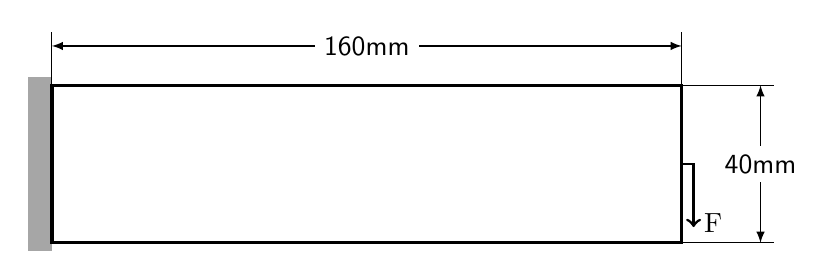
\begin{tikzpicture}
        \draw[fill,color=gray!70] (0,-0.1) rectangle (-0.3,2.1);
        \node [align=center, body,line width=1.2pt,minimum height=2cm,minimum width=8cm,anchor=south west] (body1) at (0,0) {};
        \draw (body1.south east) -- ++(1,0) coordinate (D1) -- +(5pt,0);
        \draw (body1.north east) -- ++(1,0) coordinate (D2) -- +(5pt,0);
        \draw [dimen] (D1) -- (D2) node {40mm};

        \draw (body1.north west) -- ++(0,0.5) coordinate (D1) -- +(0,5pt);
        \draw (body1.north east) -- ++(0,0.5) coordinate (D2) -- +(0,5pt);
        \draw [dimen] (D1) -- (D2) node {160mm};
        \draw[->,line width=1pt] (8,1) -- (8.15,1) -- (8.15,0.2);
        \node (arrowhead) at (8.4,0.25) {F};
    \end{tikzpicture} \newline
  }
  \caption{Cantilever beam problem before topology optimization.}
  \label{fig:CantBeam1}
\end{figure}

\begin{figure}
  \centering
  \begin{subfigure}{\textwidth}
    \resizebox{1\textwidth}{!}{
      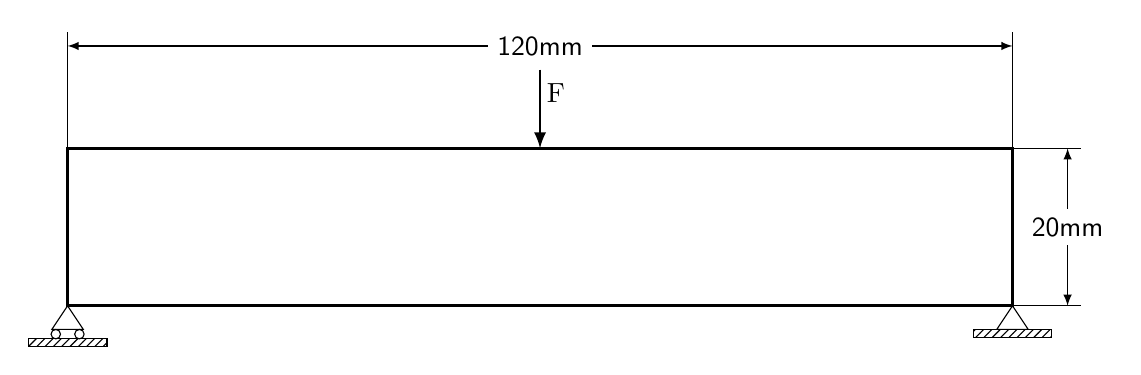
\begin{tikzpicture}[>=latex]
        \draw[line width=1.2pt] (-6,0) rectangle (6,2);
          \draw (6,0) -- ++(0.7,0) coordinate (D1) -- +(5pt,0);
          \draw (6,2) -- ++(0.7,0) coordinate (D2) -- +(5pt,0);
          \draw [dimen] (D1) -- (D2) node {20mm};
          \draw (-6,2) -- ++(0,1.3) coordinate (D3) -- +(0,5pt);
          \draw (6,2) -- ++(0,1.3) coordinate (D4) -- +(0,5pt);
          \draw [dimen] (D3) -- (D4) node {120mm};

        \draw (-6,0) -- (-6.2,-0.3) -- (-5.8,-0.3) -- cycle;
        \draw (-6.15,-0.36) circle (0.06);
        \draw (-5.85,-0.36) circle (0.06);
        \node [marked body,minimum height=0.1cm,minimum width=1cm,anchor=center] at (-6,-0.42-0.05) {};

        \draw (6,0) -- (6.2,-0.3) -- (5.8,-0.3) -- cycle;
        \node [marked body,minimum height=0.1cm,minimum width=1cm,anchor=center] at (6,-0.35) {};

        \draw[->,line width=1pt] (0,3) -- (0,2);
        \node (arrowhead) at (0.2,2.7) {F};
      \end{tikzpicture}
    }
    \caption{Full beam}
    \label{fig:FullMBB}
  \end{subfigure}
  \begin{subfigure}{0.5\textwidth}
    \hfill
    \resizebox{1\textwidth}{!}{
      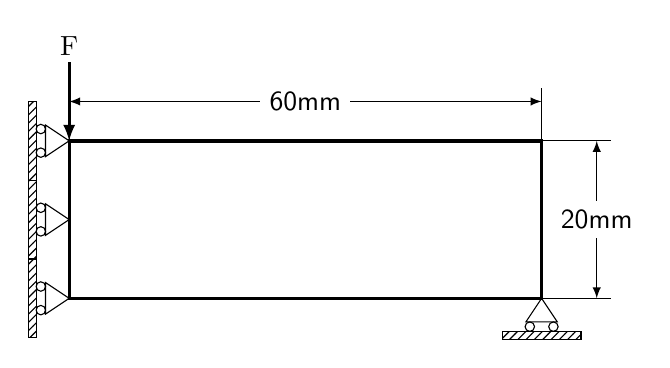
\begin{tikzpicture}[>=latex]
        \draw[line width=1.2pt] (0,0) rectangle (6,2);
        \draw (6,0) -- ++(0.7,0) coordinate (D1) -- +(5pt,0);
        \draw (6,2) -- ++(0.7,0) coordinate (D2) -- +(5pt,0);
        \draw [dimen] (D1) -- (D2) node {20mm};
        \draw (0,2) -- ++(0,0.5) coordinate (D3) -- +(0,5pt);
        \draw (6,2) -- ++(0,0.5) coordinate (D4) -- +(0,5pt);
        \draw [dimen] (D3) -- (D4) node {60mm};

        \draw (0,2) -- (-0.3,2.2) -- (-0.3,1.8) -- cycle;
        \draw (-0.36,2.15) circle (0.06);
        \draw (-0.36,1.85) circle (0.06);
        \node [marked body,minimum height=1cm,minimum width=0.1cm,anchor=center] at (-0.42-0.05,2) {};

        \draw (0,1) -- (-0.3,1.2) -- (-0.3,0.8) -- cycle;
        \draw (-0.36,1.15) circle (0.06);
        \draw (-0.36,0.85) circle (0.06);
        \node [marked body,minimum height=1cm,minimum width=0.1cm,anchor=center] at (-0.42-0.05,1) {};

        \draw (0,0) -- (-0.3,0.2) -- (-0.3,-0.2) -- cycle;
        \draw (-0.36,0.15) circle (0.06);
        \draw (-0.36,-0.15) circle (0.06);
        \node [marked body,minimum height=1cm,minimum width=0.1cm,anchor=center] at (-0.42-0.05,0) {};
        
        \draw (6,0) -- (6.2,-0.3) -- (5.8,-0.3) -- cycle;
        \draw (6.15,-0.36) circle (0.06);
        \draw (5.85,-0.36) circle (0.06);
        \node [marked body,minimum height=0.1cm,minimum width=1cm,anchor=center] at (6,-0.42-0.05) {};

        \draw[->,line width=1pt] (0,3) -- (0,2);
        \node (arrowhead) at (0,3.2) {F};
      \end{tikzpicture}
    }
    \caption{Half beam}
    \label{fig:HalfMBB}
  \end{subfigure}
  \caption{Messerschmitt-Bolkow-Blohm (MBB) beam problem}
  \label{fig:MBBBeam}
\end{figure}


In the rest of this chapter, the compliance will be defined as:
  \begin{align} \label{eqn:compliance}
    & C = \bm{u}^T\bm{K}\bm{u} = \bm{f}^T\bm{K}^{-1}\bm{f} 
  \end{align}
i.e. twice the strain energy of the system, where $\bm{K}$ is the stiffness matrix assembled from element stiffness matrices, $\bm{u}$ is the displacement vector of all the degrees of freedom of the ground mesh, such that $u_i$ corresponds to the $i^{th}$ degree of freedom of the ground mesh, and $\bm{f}$ is the load vector assembled from surface and point loads. The relationship between the global and element stiffness matrices is given by:
  \begin{gather} \label{eqn:assembly}
    \bm{K} = \sum\limits_e \rho_e(P(x_e)) \bm{K}_e \\
    \rho_e(x_e) = (1-x_{min})x_e + x_{min}
  \end{gather}
where $\bm{K}_e$ is the element stiffness matrix of element $e$, which describes the relationship between the degrees of freedom inside element $e$, and such that the $(i,j)$th entry of $\bm{K}_e$ is 0 if either degree of freedom $i$ or $j$ is not in element $e$, $P$ is the penalty function with a penalty value $p$, and $x_{min}$ is chosen to be a small value, e.g. 1e-3, to stop $\bm{K}$ from becoming singular when a node is not part of any solid element.

\section{Literature review}

Some efforts can be found in literature towards decreasing the computational burden of continuation SIMP and topology optimization at large. For instance, approximate reanalysis via reusing the stiffness matrix decomposition in direct linear solvers was proposed by Amir et al. \cite{Amir2009}. Later, approximate analysis via reusing the preconditioner in the preconditioned conjugate gradient (PCG) algorithm was also successfully applied to solve compliance problems \citep{Amir2015}. The decomposition reuse approach was then extended to approximately solve the eigenvalue problem found in topology optimization of oscillating systems \citep{Zheng2017}. Use of multi-resolution meshes and adaptive mesh refinement can also be found in topology optimization literature. For instance, Amir et al. \cite{Amir2014} used a geometric multigrid preconditioner in the PCG algorithm based on a multi-resolution mesh. Adaptive mesh refinement can also be found in numerous old and recent works, e.g. \cite{Maute1995,Maute1997,Stainko2006,Wang2010a,Wang2010a,Bruggi2011,Wang2013,Wang2014,SalazardeTroya2018,Lambe2018}.

A few works also studied some penalty adaptation routines. \cite{Dadalau2009} provided a way to adapt the penalty step which was used along with a variant of the optimality criteria method for VCCM problems. More specifically, \cite{Dadalau2009} set the penalty in each iteration such that it maximizes the ratio of the standard deviation of elements' fractional volumes, $\sigma(v_e x_e)$, and the strain energy, i.e. half the compliance. Maximizing this ratio is supposed to maximize the closeness to a binary solution, without compromising the compliance too much. However, there are two questionable points in this approach, beside not having a proof. Firstly, the standard deviation of elements' fractional volumes is not an accurate measure of how binary a solution is; it is a measure of spread around the mean. This means that the direction in which the standard deviation increases for any one element is always away from the mean. For instance, let the volume of each element be $1.0$, and let all elements have $x_e = 0.3 \quad \forall e$, therefore the mean is $0.3$ and standard deviation is $0$. Making one $x_e = 0.5$, i.e. clearly more fractional, will increase the standard deviation to a strictly positive value, thus falsely claiming that the new solution is closer to a 0-1 design. When the volume constraint is active, the mean value of $x_e$, weighted by the element volumes, is exactly the volume fraction. The second problem with the approach proposed by \cite{Dadalau2009} is that as shown in their experiments, the penalty value $p$ is allowed to freely increase or decrease with no control over the final penalty, which means that SIMP's (or RAMP's) property of converging to a binary solution for VCCM problems with a high penalty is lost.

Another penalty adaptation approach was proposed by \cite{GaoXingjun2017} for buckling constrained compliance minimization problems. \cite{GaoXingjun2017} chose the penalty in each subproblem to promote a certain amount of constraint violation such that the eigenvalue constraint is violated by 0.1 if possible while maintaining an increasing penalty. This was motivated by the observation that for low penalty values, all the buckling load factors are typically over the threshold, so the stability constraint is not active and does not contribute to the optimization process. However, when the penalty increases, the violated stability constraints require a re-distribution of the material, which when the problem is non-convex, may converge to a bad and/or infeasible solution. The heuristic proposed was shown to improve the stability of the solution, though still infeasible, at the expense of a higher compliance.

However most notably, \cite{Rojas-Labanda2015} tried to reduce the number of FEA simulations needed by CSIMP for generic topology optimization problems using a number of alternative approaches, the most significant of which was the \textit{automatic} continuation SIMP (Auto-CSIMP). In auto-CSIMP the penalty $p$ is treated as a variable and a constraint is defined such that it is feasible only when $p = p_{max}$. A nonlinear equality (or inequality) constraint $g(p;\mu) = 0$ (or $\leq 0$) is added, where $\mu$ is a hyperparameter, and the whole problem is solved using a first order NLP solver which solves for $p$ and $\bm{x}$ simultaneously, using linear approximation of the nonlinear constraints, such as the interior point optimizer IPOPT \citep{Wachter2006}. The main purpose of this additional constraint is to stall the convergence of the algorithm achieving a similar effect as the original CSIMP. While this method was shown to successfully decrease the number of simulations needed to converge, there are a few questionable points about the algorithm. Firstly, the choice of $g(p;\mu)$ and its hyperparameter $\mu$ seem largely arbitrary with the exception of being a decreasing function in $p$ which was derived from Newton's method applied on the KKT conditions of the barrier problem used in IPOPT. However, the analysis of the number of iterations needed to reach the final penalty for different functions $g$ and values of $\mu$ is not accurate since it assumes a fixed step size of $\alpha = 1$ in Newton's method. So it is not clear that the choice of $g(p;\mu)$ or its hyperparameter thereof will never result in IPOPT satisfying the penalty constraint too quickly thus approaching the behavior of a single penalty SIMP. In the paper by \cite{Wachter2006} which describes the algorithm used in IPOPT, the actual step $\alpha_k$ is influenced by the search direction in $[\bm{x}; p]$, which is a function of: 
  \begin{enumerate}[label=(\arabic*)]
    \item the Hessian of the Lagrangian of the barrier problem with respect to $[\bm{x}; p]$, 
    \item the Jacobian of the constraints with respect to $[\bm{x}; p]$, and 
    \item the initial primal and dual solutions. 
  \end{enumerate}
  Moreover, $\alpha_k$ is ultimately determined by how the objective and constraints change along the search direction during the backtracking line search for [$\bm{x}; p]$ combined, as well as the line search's stopping criteria. Additionally, the search direction can itself be influenced by the step size in case the second order correction step is performed. The influence of factors like the number of elements, the volume of each element, the Young's modulus and Poisson's ratio of the material on the step size that IPOPT takes was not studied and is indeed difficult to measure; so the risk of premature convergence of the penalty constraint exists. Secondly, it seems unclear whether using a different NLP solver or improving the existing IPOPT solver will result in a better or worse Auto-CSIMP. While Auto-CSIMP is, in theory, possible to use for any topology optimization problem and was shown to outperform the traditional MMA-based CSIMP with a large penalty step by \cite{Rojas-Labanda2015}, the design space for MMA-based CSIMP algorithms has not been fully explored yet.

\section{Penalty adaptation} \label{sec:adaptive_penalty}

  In every CSIMP subproblem, an NLP is solved using a certain penalty value $p$ until convergence before moving on to the next penalty value. When using the KKT stopping criteria, at every penalty step, there is at least 1 FEA simulation to be performed in order to check for convergence. However in certain phases of CSIMP, e.g. near convergence, changing the value of $p$ is not likely to change the solution or the objective much. Therefore, one improvement that can be employed is to use the last solution $\bm{u}$ from the last FEA simulation of the previous subproblem with the new penalty value to estimate the change in the objective value. If the change is large enough, the subproblem can be solved, otherwise, the penalty can be incremented right away saving unnecessary FEA simulations. The new subproblem's tolerance can be used as this criteria. This provides a simple way to adapt the penalty step not to perform unnecessary FEA simulations. 

  To develop some mathematical intuition for this approach, let's assume the relative change in the objective stopping criteria is used for the MMA, together with solution feasibility. One can then attempt to estimate the effect of $p$ on the optimal value $C^*$, through a first order Taylor series expansion of $C^*(p)$, which is the optimal value of $C$ for each penalty value $p$. Assuming that the local optimal solution $\bm{x}^*$ is a KKT point of the subproblem at the current $p$ and that the optimal primal-dual solution, the objective and constraints are continuous and differentiable functions of $p$, it is possible to prove that:
  \begin{align} \label{eqn:fullderivative}
    & \frac{dC^*(p)}{dp} = \frac{\partial C}{\partial p} - \sum_i{\lambda_i \frac{\partial h_i}{\partial p}}
  \end{align}
  where $h_i$ is the $i^{th}$ constraint, and $\lambda_i$ is the corresponding Lagrangian multiplier. For the VCCM problem, this is simply $\frac{dC^*(p)}{dp} = \frac{\partial C}{\partial p}$ since the constraints are not a function of $p$. This also means that the value of $p$ does not change the feasibility status of a solution.

  \begin{proof}
    Let $\bm{x}(p)$ now denote the optimal solution $\bm{x}^*$ given a certain value of $p$. The KKT conditions guarantee that:
    \begin{align} \label{eqn:kkt1}
      & -\nabla_{\bm{x}} C + \sum_i \lambda_i \nabla_{\bm{x}} h_i = \bm{0}
    \end{align}
    The full derivative of the optimal compliance $C^*(p) = C(\bm{x}(p), p)$ with respect to $p$ is:
    \begin{align}
      & \frac{dC^*(p)}{dp} = \frac{\partial C(p)}{\partial p} + \nabla_{\bm{x}} C \cdot \frac{d\bm{x}(p)}{dp}
    \end{align}
    Taking the dot product of the LHS and RHS of equation \ref{eqn:kkt1} with $\frac{d\bm{x}(p)}{dp}$ and adding $-\frac{\partial C}{\partial p}  + \sum_i \lambda_i \frac{\partial h_i}{\partial p}$ to both sides, one can show that:
    \begin{align} \label{eqn:presimpl_fullderivative}
      & -\frac{dC^*}{dp} + \sum_i \lambda_i \frac{dh^*_i}{dp} = -\frac{\partial C}{\partial p}  + \sum_i \lambda_i \frac{\partial h_i}{\partial p}
    \end{align}
    where $h^*_i = h_i(\bm{x}(p), p)$.
    Furthermore, the complementarity slackness property of the KKT solution specifies that:
    \begin{align} \label{eqn:compl_slackness}
      & \lambda_i(p) h_i(\bm{x}(p), p) = 0
    \end{align}
    Using the product rule:
    \begin{align}
      & \frac{d\lambda_i(p)}{dp} h_i(\bm{x}(p), p) + \lambda_i(p) \frac{d h_i(\bm{x}(p), p)}{dp} = 0
    \end{align}
    Multiplying both sides by $\lambda_i(p)$ and using equation \ref{eqn:compl_slackness}, one can show that:
    \begin{align}
      & \lambda_i(p)^2 \frac{d h_i(\bm{x}(p), p)}{dp} = 0
    \end{align}
    so either $\lambda_i(p) = 0$ or $\frac{d h_i(\bm{x}(p), p)}{dp} = 0$. In other words, equation \ref{eqn:presimpl_fullderivative} simplifies into equation \ref{eqn:fullderivative}. \textit{This completes the proof}.
  \end{proof}

  Let $\bm{u}$, $\bm{x}$ and $p$ be independent variables, as in Simultaneous Analysis and Design (SAND). The partial derivative of $C$ with respect to $p$ is:
  \begin{align}
    & \frac{\partial{C(\bm{u}, \bm{x}, p)}}{\partial{p}} = \bm{u}^T \frac{\partial \bm{K}(\bm{x}, p)}{\partial p} \bm{u} \\
    & \frac{\partial \bm{K}(\bm{x}, p)}{\partial p} = \sum\limits_e log(x_e) \times x_e^p \times \bm{K}_e
  \end{align}
  Note that this function is discontinuous at any point where some $x_e = 0$. However, using L'Hopital's rule on $\frac{log(x_e)}{1/x_e^p}$, $\lim_{x_e \to 0} log(x_e) \times x_e^p = -\frac{x_e^p}{p} = 0$. Therefore, $\frac{\partial \bm{K}}{\partial p}$ can be numerically defined as:
  \begin{align}
    \frac{\partial \bm{K}}{\partial p} = \sum\limits_e \Gamma_e \times \bm{K}_e \\ 
    \Gamma_e = \begin{cases}
      log(x_e) \times x_e^p & x_e \geq \epsilon \\
      0 & x_e < \epsilon
    \end{cases}
  \end{align}
  for some small $\epsilon$. 

  Incidentally, $\frac{\partial{C(\bm{u}, \bm{x}, p)}}{\partial{p}}$, when $\bm{u}$ is treated as a variable, is equal to $-\frac{\partial C(\bm{x}, p)}{\partial p}$ when treating $\bm{u}$ as a function of $\bm{x}$ and $p$, as in Nested Analysis and Design (NAND). Since $\bm{u}(\bm{x}, p)$ is implicitly defined by:
  \begin{align}
    & \bm{K}(\bm{x}, p) \bm{u}(\bm{x}, p) = \bm{f}
  \end{align}
  then:
  \begin{align}
    & \frac{\partial \bm{K}}{\partial p} \bm{u} + \bm{K} \frac{\partial \bm{u}}{\partial p} = 0 \nonumber \\
    & \frac{\partial \bm{u}}{\partial p} = -\bm{K}^{-1} \frac{\partial \bm{K}}{\partial p} \bm{u}
  \end{align}
  Hence, the partial derivative of $C(\bm{x}, p) = \bm{u}(\bm{x}, p)^T \bm{K}(\bm{x}, p) \bm{u}(\bm{x}, p)$ with respect to $p$ is:
  \begin{align}
    \label{eqn:partialCpartialp}
    \frac{\partial C(\bm{x}, p)}{\partial p} & = 2 \bm{u}^T \bm{K} \frac{\partial \bm{u}}{\partial p} + \bm{u}^T \frac{\partial \bm{K}}{\partial p} \bm{u} \nonumber \\
    & = -\bm{u}^T \frac{\partial \bm{K}}{\partial p} \bm{u}
  \end{align}
  Since $x_e \leq 1$, and $\bm{K}_e$ is positive semi-definite for all $e$, the above term is non-negative. In this chapter, the NAND framework is used.

  Assuming the first order approximation, it is also possible to choose the penalty step $\Delta p_k$ such that the approximate compliance:
  \begin{align}
    \tilde{C}_{k} = C(\bm{u}_{k-1}, \bm{x}_{k-1}, p_{k-1} + \Delta p_k) \approx C_{k-1} + \frac{\partial C}{\partial p}(\bm{u}_{k-1}, \bm{x}_{k-1}, p_{k-1}) \times \Delta p_k
  \end{align}
  satisfies inequality (\ref{eqn:tolerance})\begin{align}
    \label{eqn:tolerance}
    |C_{k-1} - C_{k}| / |C_{k-1}| < tol 
  \end{align}
  for some tolerance  $tol$. Choosing $\Delta p$ such that:
  \begin{align}
    |C_{k-1} - \tilde{C}_{k}| / |C_{k-1}| = \beta \times tol
  \end{align}
  for some $\beta \geq 1$, we get:
  \begin{align}
    \label{eqn:blind_adaptive_step}
    \Biggl| \frac{\partial C}{\partial p}\Biggr| \frac{\Delta p}{|C_{k-1}|} = \beta \times tol \nonumber \\
    \Delta p = \frac{\beta \times tol \times |C_{k-1}|}{| \partial C / \partial p|}
  \end{align}

  On the other hand, using blind penalty adaptation with $\Delta p = \Delta p_0 \times n$ for $n \in \mathbb{N}$, where $\Delta p_0$ is the fixed step in CSIMP, the benefit of penalty adaptation can only be observed when $n > 1$, that is some subproblem is skipped because it is deemed unnecessary. The condition for $n > 1$ is:
  \begin{align}
    \Delta p_0 \leq \frac{tol \times |C_{k-1}|}{|\partial C / \partial p|}    
  \end{align}
  More generally, the condition for $i$ subproblems to be skipped, i.e. $\Delta p \geq \Delta p_0 \times (i + 1)$ is:
  \begin{align}
    \Delta p_0 \times i \leq \frac{tol \times |C_{k-1}|}{| \partial C / \partial p|}    
  \end{align}
  Not surprisingly, the penalty adaptation trick can be observed to be more effective in skipping subproblems for small $\Delta p_0$ and large $tol$. While the intuition above was developed using the relative change in objective value, computational experiments show a significant reduction in the number of FEA simulations from skipping subproblems when using the more rigorous KKT stopping criteria.

\section{Test Problems} \label{sec:test_problems}

  \begin{figure}
  \centering
  \resizebox{\textwidth}{!}{
    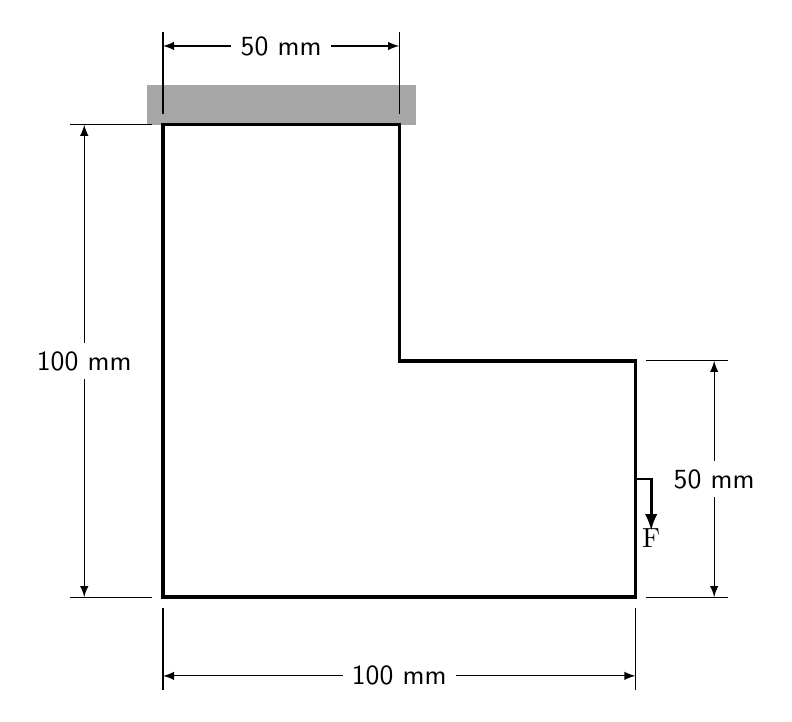
\begin{tikzpicture}[>=latex]
        \draw[fill,color=gray!70] (-0.2,2) rectangle (3.2,2.5);
        \draw[line width=1.2pt] (0, 2) node(nodeA){} -- (3, 2) node(nodeB){} -- (3, -1) -- (6, -1) node(nodeC){} -- (6, -4) node(nodeD){} -- (0, -4) node(nodeE){} -- cycle;
        
        \draw (nodeA) -- ++(0,1) coordinate (D1) -- +(0,5pt);
        \draw (nodeB) -- ++(0,1) coordinate (D2) -- +(0,5pt);
        \draw [dimen] (D1) -- (D2) node {50 mm};

        \draw (nodeA) -- ++(-1,0) coordinate (D1) -- +(-5pt,0);
        \draw (nodeE) -- ++(-1,0) coordinate (D2) -- +(-5pt,0);
        \draw [dimen] (D1) -- (D2) node {100 mm};

        \draw (nodeC) -- ++(1,0) coordinate (D1) -- +(5pt,0);
        \draw (nodeD) -- ++(1,0) coordinate (D2) -- +(5pt,0);
        \draw [dimen] (D1) -- (D2) node {50 mm};

        \draw (nodeE) -- ++(0,-1) coordinate (D1) -- +(0,-5pt);
        \draw (nodeD) -- ++(0,-1) coordinate (D2) -- +(0,-5pt);
        \draw [dimen] (D1) -- (D2) node {100 mm};

        \draw[->,line width=1pt] (6,-2.5) -- (6.2,-2.5) -- (6.2,-3.15);
        \node (arrowhead) at (6.2,-3.25) {F};
    \end{tikzpicture} \newline
  }
  \caption{L-shaped beam problem}
  \label{fig:LBeam}
\end{figure}


  There is a wide array of test problems used in literature to evaluate topology optimization algorithms. In the majority of papers, a few test problems are used to demonstrate the effect of algorithms, e.g. \cite{Huang2010a}, \cite{Stolpe2001a}, and \cite{SalazardeTroya2018}. \cite{Valdez2017} compiled a list of linearly elastic 2D structures commonly used as test problems in literature. Another set of problems for compliant mechanisms was also proposed by \cite{Deepak2009}. However, perhaps the largest set of benchmark problems ever used in literature was by \cite{Rojas-Labanda2015a, Rojas-Labanda2015}. Rojas-Labanda et al. used a library of 225 minimum compliance problems, 135 minimum volume and 150 compliant mechanism design problems in \cite{Rojas-Labanda2015a}. The same authors seem to have used a subset of this library in \cite{Rojas-Labanda2015}. In this chapter, three 2D VCCM problems, shown in Figures \ref{fig:CantBeam1}-\ref{fig:LBeam}, and 1 3D VCCM problem are used to highlight the effect of penalty adaptation. A possible future work is to perform a more extensive study on a larger library of problems.
  
  The first test problem is the 2D cantilever beam problem, Figure \ref{fig:CantBeam1}, which was solved by \cite{Huang2010a} to benchmark soft-kill BESO against CSIMP. The second test problem is the MBB problem, Figure \ref{fig:MBBBeam}, was solved in the classical paper by \cite{Sigmund2001}. Due to the symmetry of the problem, the problem in Fig. \ref{fig:FullMBB} is typically reduced to the problem in \ref{fig:HalfMBB} to reduce the area of the topology to be optimized. The third test problem is the L-beam problem, Figure \ref{fig:LBeam}, which was taken from the book by \cite{Bendsoe2004}. These three problems are all part of the 2D collection made by \cite{Valdez2017}. Finally, a 3D cantilever beam variant of the first test problem will be tested with a ground mesh of dimensions $60 \times 20 \times 20$.

  In the 2D test problems, a ground mesh of plane stress quadrilateral elements is used, where each element is a square of side length $1\text{mm}$, and a sheet thickness of $1 \text{mm}$. In the 3D cantilever beam problem, hexahedral elements are used, where each element is a cube of side length $1\text{mm}$. Linear isoparameteric interpolation functions are used in the MBB, L-beam and 3D cantilever beam problems, and quadratic isoparameteric interpolation functions are used in the 2D cantilever beam problem. The 2D cantilever beam problem with a low volume fraction and linear interpolation functions was found to produce some extremely ill-conditioned geometries with corner contacts, hence the use of quadratic interpolation functions to achieve better accuracy in the FEA simulations. A Young's modulus of 1 MPa and Poisson's ratio of 0.3 are used in all the problems. A chequerboard density filter was used with a radius of 2 mm. The weights were calculated using the method described by \cite{Huang2010a}.

\section{Implementation} \label{sec:implementation}

  \subsection{Finite element analysis}

  All the topology optimization algorithms described in this chapter were implemented using the Julia programming language \citep{Bezanson2014} for handling generic unstructured, isoparameteric meshes. Finite element analysis was done with the help of the finite element tooling package JuAFEM.jl \footnote{https://github.com/KristofferC/JuAFEM.jl}. A direct Cholesky factorization based linear system solver for sparse matrices was used from SuiteSparse \footnote{http://faculty.cse.tamu.edu/davis/suitesparse.html} wrapped in Julia. The value of $x_{min}$ used was $0.001$ for all problems and algorithms since this is the standard value used in literature.

  \subsection{Optimization}

  The original MMA algorithm by \cite{Svanberg1987} was implemented and used to solve the SIMP subproblems. MMA parameters of $s_{init} = 0.5$, $s_{incr} = 1.2$ and $s_{decr} = 0.7$ were used as defined in the paper by \cite{Svanberg1987}. The dual problem of the convex approximation was solved using a log-barrier box-constrained nonlinear optimization solver, where the barrier problem was solved using the nonlinear CG algorithm for unconstrained nonlinear optimization \citep{Nocedal2006} as implemented in Optim.jl \footnote{https://github.com/JuliaNLSolvers/Optim.jl} \citep{KMogensen2018}. The nonlinear CG itself used the line search algorithm from Hager et al. \cite{Hager2006} as implemented in LineSearches.jl \footnote{https://github.com/JuliaNLSolvers/LineSearches.jl}.

  The stopping criteria used was similar to the one adopted by the KKT solver, IPOPT \citep{Wachter2006}. This stopping criteria is less scale sensitive than the KKT residual as it scales down the residual by a value proportional to the mean absolute value of the Lagrangian multipliers. Let the optimization problem be:
      \begin{mini!}|l|[3]
        {\bm{x}}{f(\bm{x})}{}{}
        \addConstraint {\quad \bm{c}(\bm{x}) \leq \bm{0}}{}
        \addConstraint {\quad 0 \leq x_e \leq 1}{\quad \forall e}
      \end{mini!}
  Let $\bm{\lambda}$ be the vector of Lagrangian multipliers of the nonlinear constraints, $\bm{z}_-$ be the vector of Lagrangian multipliers of the $\geq$ bound constraints, and $\bm{z}_+$ be the vector of Lagrangian multipliers of the $\leq$ bound constraints. The termination criteria used was:
    \begin{align}
      \max\Biggl\{\frac{||\nabla f(\bm{x}) + \nabla \bm{c}(\bm{x}) \bm{\lambda} + (\bm{z_+} - \bm{z_-})||_\infty}{s_d}, ||\bm{c}(\bm{x})_+||_\infty \Biggr\} \leq tol \\
      s_d = \max\Biggl\{s_{max}, \frac{||\bm{\lambda}||_1 + ||\bm{z_+} + \bm{z_-}||_1}{m + n} \Biggr\} / s_{max}
    \end{align}
  where $\bm{c}_+$ is the element-wise maximum of $\bm{c}$ and 0, and $s_{max}$ is a constant parameter. A value of $s_{max} = 100$ was used by \cite{Wachter2006} and the same is done in this work.

\section{Evaluating SIMP} \label{sec:evaluating_simp}

  There are a number of difficulties that one faces when trying to fairly assess the performance of SIMP variants to solve the VCCM problem:
  \begin{enumerate}
    \item The solution generated by SIMP is a continuous one, where $x_e$ is allowed to take fractional values. Therefore, the objective value is that of the continuous approximation of the problem. Moreover, $x_{min}$ and $P$ can affect the objective value differently for different ground mesh geometries.
    \item Obtaining a discrete solution from a continuous one can be done in different ways:
      \begin{enumerate}
        \item The solution can be rounded. This approach carries the risk of obtaining an infeasible solution after rounding even if the continuous solution was feasible.
        \item A projection function such as the regularized Heaviside projection function $f(x) = 1 - e^{\beta x} + x e^{-\beta}$ \citep{Guest2004} can be used to make the projected solution closer to a binary one. This method has the disadvantage of increasing the non-convexity of the optimization problem, requiring more iterations to converge, for $\beta > 0$. The regularized Heaviside function is the identity function when $\beta = 0$, and it gradually approximates the Heaviside step function as $\beta \to \infty$. A continuation over $\beta$ is therefore typically used. From experiments, using a high value of $\beta$ can cause numerical difficulties for the NLP solver because the slope at $x \approx 0$ becomes very high. Moreover, a very high value of $\beta$ is often required to get a near-binary solution.
        \item A subset of the elements can be selected based on their sorted $x_e$ values. In VCCM problems, this can be done by selecting the top $100V\%$ of the elements by $x_e$. However, for other constraints which require solving an FEA simulation to evaluate the feasibility of a solution, this approach is not straight forward to generalize. For constraints which are known to be satisfied with a full grid design, a bisection search can be used, adding or removing elements until a feasible binary solution is obtained.
      \end{enumerate}
      For the sake of this chapter, the regularized Heaviside projection was used together with the element selection method, where the top $100V\%$ elements were selected as per the projected filtered densities, then the discrete objective value was computed.
    \item After obtaining a discrete solution, the solution can exhibit chequerboard patterns, disconnected or undesired thin features. These are mostly visual features for which no metric in topology optimization literature exists as far as we know.
    \item Some SIMP variants can converge quickly to a solution with a good continuous objective value but a bad or undefined discrete objective value, due to disconnectivity or ill-conditioned geometries, e.g. corner contacts. For example in the VCCM problem, using a single low penalty value can generally lead to a lower continuous objective value, closer the lower bound which is the optimal value at $p = 1$, but the discrete design's objective value can be either infeasible or suboptimal.
  \end{enumerate}
  In SIMP literature, algorithms seem to be compared using their continuous objective values. Therefore, we do the same in this chapter. However, an additional metric will be added to measure how fractional a solution is. A more fractional solution is arguably a less trusted one since the continuous and discrete objectives are likely to be far apart. The measure of how fractional a solution is to be used in this chapter will be:
  \begin{align}
    \% frac = \frac{2 \sum\limits_e \min(x_e, 1 - x_e) \times v_e}{\sum\limits_e v_e} \times 100 \%
  \end{align}
  which is $0\%$ when a solution is fully binary, $100\%$ when a solution is all $0.5$ and it weighs the fractional part of a variable by the volume of the corresponding element. The fractionness of the solution will be evaluated using the projected filtered densities.
 
  In the following section, $\text{C-Obj}$ will refer to the objective value of the continuous optimal solution. This includes the effect of $x_{min}$, the density filter and projection. One additional metric to be used is the discrete design's objective value ($\text{D-Obj}$) after selecting the top $100V\%$ of the elements by their projected and filtered densities, and removing the void elements completely.

\section{Results and Discussion} \label{sec:penalty_adaptation_results}

  \subsection{Fixed tolerance}

  \begin{table}[H]
\centering
\tabcolsep=0.09cm
% table caption is above the table
\caption{The problem type and parameter settings of the experiments with continuation SIMP with a fixed tolerance.}
\label{tab:exp_params}
\begin{tabular}{|l|l|l|l|l||l|l|l|l|l|}
\hline\noalign{\smallskip}
Exp & Problem & $V$ & $tol$ & $\Delta p_0$ & Exp & Problem & $V$ & $tol$ & $\Delta p_0$ \\
\hline
1 & \multirow{ 8 }{*}{CantBeam} & \multirow{ 4 }{*}{0.3} & \multirow{ 2 }{*}{0.01} & 0.1 & 17 & \multirow{ 8 }{*}{LBeam} & \multirow{ 4 }{*}{0.3} & \multirow{ 2 }{*}{0.01} & 0.1\\
2 & & & & 0.05 & 18 & & & & 0.05\\
3 & & & \multirow{ 2 }{*}{0.0001} & 0.1 & 19 & & & \multirow{ 2 }{*}{0.0001} & 0.1 \\
4 & & & & 0.05 & 20 & & & & 0.05 \\
5 & & \multirow{ 4 }{*}{0.5} & \multirow{ 2 }{*}{0.01} & 0.1 & 21 & & \multirow{ 4 }{*}{0.5} & \multirow{ 2 }{*}{0.01} & 0.1 \\
6 & & & & 0.05 & 22 & & & & 0.05 \\
7 & & & \multirow{ 2 }{*}{0.0001} & 0.1 & 23 & & & \multirow{ 2 }{*}{0.0001} & 0.1 \\
8 & & & & 0.05 & 24 & & & & 0.05 \\
\hline
9 & \multirow{ 8 }{*}{HalfMBB} & \multirow{ 4 }{*}{0.3} & \multirow{ 2 }{*}{0.01} & 0.1 & 25 & \multirow{ 8 }{*}{3D CantBeam} & \multirow{ 4 }{*}{0.3} & \multirow{ 2 }{*}{0.01} & 0.1 \\
10 & & & & 0.05 & 26 & & & & 0.05 \\
11 & & & \multirow{ 2 }{*}{0.0001} & 0.1 & 27 & & & \multirow{ 2 }{*}{0.0001} & 0.1 \\
12 & & & & 0.05 & 28 & & & & 0.05 \\
13 & & \multirow{ 4 }{*}{0.5} & \multirow{ 2 }{*}{0.01} & 0.1 & 29 & & \multirow{ 4 }{*}{0.5} & \multirow{ 2 }{*}{0.01} & 0.1 \\
14 & & & & 0.05 & 30 & & & & 0.05 \\
15 & & & \multirow{ 2 }{*}{0.0001} & 0.1 & 31 & & & \multirow{ 2 }{*}{0.0001} & 0.1 \\
16 & & & & 0.05 & 32 & & & & 0.05 \\
\noalign{\smallskip}\hline
\end{tabular}
\end{table}

  \begin{table}
\centering
\tabcolsep=0.09cm
% table caption is above the table
\caption{This table shows the effect of penalty adaptation on CSIMP. The table shows the results of the experiments studying the effect of solution reuse on: 1) the number of FEA simulations (Sims) required by CSIMP, 2) the final objective of the continuous NLP at $p = 5$ (C-Obj), 3) the objective value of the rounded discrete solution (D-Obj), and 4) the percentage of fractionness (\% frac). The parameters of each experiment are described in Table \ref{tab:exp_params}}
\label{tab:csimp_reuse}
\begin{tabular}{|l|l|l|l|l||l|l|}
\hline\noalign{\smallskip}
Exp & \multicolumn{3}{c||}{\textbf{Fixed $\Delta p = \Delta p_0$}} & \multicolumn{3}{c|}{\textbf{\% Increase due to $\Delta p$ adaptation}}\\
\noalign{\smallskip}\hline\noalign{\smallskip}
& \textbf{Sims} & \textbf{C-Obj / D-Obj} & \textbf{\% frac} & \textbf{Sims} & \textbf{C-Obj / D-Obj} & \textbf{\% frac} \\
\hline
1 & 149 & 813.0/555.8 & 17.3 & -20.8 & -9.3/1.0 & -13.3 \\ 
\hline
2 &  213 & 742.2/572.4 & 14.3 & -45.1 & 1.6/-1.4 & 5.6 \\ 
\hline
3 &  291 & 720.4/549.2 & 14.1 & -18.2 & 0.5/-0.7 & 0.7 \\ 
\hline
4 &  485 & 712.5/559.9 & 13.8 & -18.1 & -0.3/0.5 & -0.7 \\ 
\hline
5 & 103 & 383.8/343.1 & 14.0 & -32.0 & -1.9/0.6 & -7.9 \\ 
\hline
6 & 149 & 382.7/338.3 & 12.4 & -53.0 & -0.1/1.7 & 6.5 \\ 
\hline
7 & 251 & 366.7/338.4 & 10.0 & -21.5 & 0.1/0.0 & 1.0 \\ 
\hline
8 & 376 & 366.9/338.0 & 9.9 & -24.5 & -0.0/0.2 & 0.0 \\ 
\hline
\hline
9 & 110 & 584.2/293.5 & 24.5 & -40.0 & 5.1/-0.4 & 2.0 \\ 
\hline
10 & 166 & 572.7/293.3 & 24.4 & -59.6 & 9.5/-0.3 & 2.9 \\ 
\hline
11 & 206 & 609.9/291.6 & 24.5 & -18.0 & 0.1/-0.1 & 0.0 \\ 
\hline
12 & 310 & 607.5/293.5 & 24.4 & -25.2 & 0.4/0.0 & 0.4 \\ 
\hline
13 & 97 & 229.6/176.7 & 19.9 & -37.1 & -5.4/-0.1 & -5.0 \\ 
\hline
14 & 137 & 229.8/176.8 & 20.0 & -54.7 & -4.7/-0.2 & -4.0 \\ 
\hline
15 & 256 & 219.3/176.5 & 18.6 & -21.9 & -0.3/-0.5 & -3.2 \\ 
\hline
16 & 339 & 217.7/176.9 & 17.8 & -17.4 & -0.2/-0.6 & 0.0 \\ 
\hline
\hline
17 & 104 & 126.8/103.4 & 10.2 & -33.7 & -2.6/-0.2 & 0.0 \\ 
\hline
18 & 148 & 128.4/102.4 & 10.4 & -52.7 & -4.4/0.7 & -3.8 \\ 
\hline
19 & 413 & 117.1/102.0 & 7.8 & -18.4 & 4.0/1.4 & 21.8 \\ 
\hline
20 & 505 & 121.8/103.5 & 9.5 & -13.7 & -0.1/0.1 & -1.1 \\ 
\hline
21 & 91 & 73.3/66.7 & 10.1 & -39.6 & 1.0/0.1 & -3.0 \\ 
\hline
22 & 133 & 72.4/66.5 & 9.5 & -56.4 & 1.2/0.3 & -2.1 \\ 
\hline
23 & 269 & 69.9/65.2 & 7.5 & -14.5 & -0.1/0.0 & -1.3 \\ 
\hline
24 & 367 & 69.9/65.3 & 7.5 & -15.5 & 0.0/-0.2 & -2.7 \\ 
\hline
\hline
25 & 63 & 17.7/13.2 & 13.0 & -61.9 & -1.7/0.0 & -2.3 \\ 
\hline
26 & 104 & 17.3/13.2 & 12.7 & -76.0 & -0.6/0.0 & 0.0 \\ 
\hline
27 & 232 & 16.3/13.3 & 10.0 & -20.3 & -1.2/-0.8 & -1.0 \\ 
\hline
28 & 299 & 16.2/13.2 & 10.0 & -23.1 & -1.9/-0.8 & -3.0 \\ 
\hline
29 & 65 & 10.7/9.3 & 13.3 & -60.0 & -0.9/0.0 & -0.8 \\ 
\hline
30 & 106 & 10.6/9.3 & 13.0 & -74.5 & 0.0/0.0 & -0.8 \\ 
\hline
31 & 214 & 10.3/9.3 & 12.3 & -22.0 & 0.0/0.0 & 0.8 \\ 
\hline
32 & 293 & 10.3/9.2 & 12.2 & -37.9 & 0.0/1.1 & -2.5 \\ 
\hline
\noalign{\smallskip}\hline
\end{tabular}
\end{table}


  The CSIMP algorithm with a fixed tolerance was tested on a number of problem instances as shown in Table \ref{tab:csimp_reuse}. The effect of the penalty adaptation on the continuous objective value (C-Obj), the discrete solution's objective value (D-Obj), the percentage of fractionness (\% frac) and the number of FEA simulations is shown below. The experiments' parameters are shown in Table \ref{tab:exp_params}. 

  A few observations can be made from the results of the experiments with a fixed tolerance:
  \begin{enumerate}
    \item Penalty adaptation consistently leads to a reduction in the number of FEA simulations in all experiments run.
    \item Decreasing $tol$ generally results in a decrease in C-Obj, $\% frac$ and the gap between C-Obj and D-Obj.
    \item In some cases where premature convergence of one subproblem due to a high $tol$ leads the algorithm to a different basin of attraction in the next subproblem, a better solution can be obtained for the higher $tol$ variant. This is observed in Exps 9 and 10 compared to Exps 11 and 12 respectively. This is due to the non-convexity of the optimization problem.
    \item Increasing $tol$ increases the efficacy of penalty adaptation in reducing the number of FEA simulations needed to converge.
    \item Reducing $\Delta p_0$ generally increases the efficacy of penalty adaptation. From equation \ref{eqn:blind_adaptive_step}, one can predict that a smaller $\Delta p_0$ leads to a smaller predicted change, which if lower than the tolerance, a subproblem will be skipped. However, it is not clear from the onset that such skipping of subproblems will lead to a saving in the number of FEA simulations or otherwise. Experiments show that the savings can indeed be significant.
    \item A reduction in the volume fraction $V$ causes a larger discrepancy between the continuous and discrete objective values. This makes sense because void elements are not completely removed in the continuous objective therefore their effect will be more obvious as their ratio increases.
  \end{enumerate}
  
  \begin{figure}
    \centering
    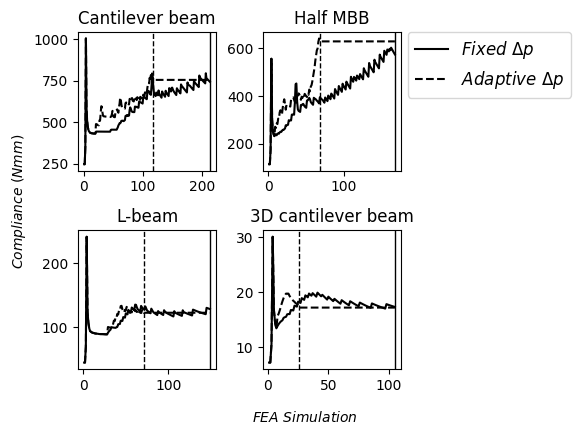
\includegraphics[width=\textwidth]{images/adaptive_csimp/convplots_csimp_03_01_80_001_ip.png}
    \caption{Convergence plots for CSIMP with and without penalty adaptation using $V = 0.3$, $tol = 0.01$, $\Delta p = 0.05$.}
    \label{fig:reuse_convplots_high_tol}
  \end{figure}
  \begin{figure}
    \centering
    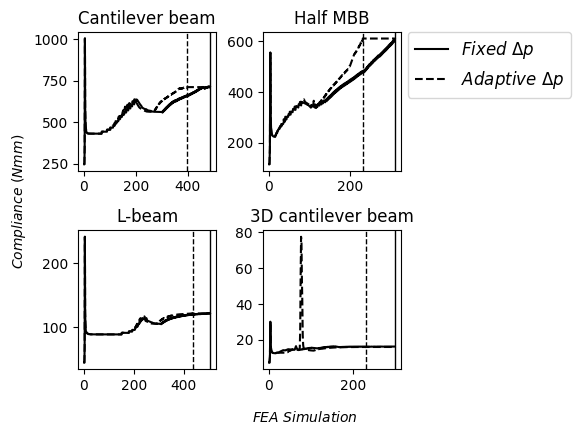
\includegraphics[width=\textwidth]{images/adaptive_csimp/convplots_csimp_03_0001_80_001_ip.png}
    \caption{Convergence plots for CSIMP with and without penalty adaptation using $V = 0.3$, $tol = 0.0001$, $\Delta p = 0.05$.}
    \label{fig:reuse_convplots_low_tol}
  \end{figure}

  Figures \ref{fig:reuse_convplots_high_tol} and \ref{fig:reuse_convplots_low_tol} show typical convergence plots for the test problems using high and low tolerances respectively with and without penalty adaptation. It is clear that the curves follow a similar pattern and converge to similar objective values but the penalty adaptation causes an acceleration to the convergence. In one case, the penalty adaptation curve had a higher peak which can be explained by the extreme changes in the objective of the current solution when skipping many subproblems optimization. 

  Overall, the results seem to suggest the need for a decreasing tolerance scheme to allow penalty adaptation to be more effective than when using a fixed low tolerance, while reaping the benefits of a low final tolerance in the objective value and reducing the \% frac of the continuous solution.

  \subsection{Decreasing tolerance}

  In the previous section, the effect of the tolerance on $\% frac$, C-Obj and D-Obj was observed. While a lower tolerance seems to have some undeniable benefits in most test problems, it is certainly more computationally expensive. It is therefore customary to use a decreasing tolerance scheme with $\theta < 1$ in Algorithm \ref{alg:cont_simp} since for low penalty values $p$ and low $\beta$, the solution is still highly fractional and therefore solving it to a low tolerance is thought to be unnecessary. Algorithm \ref{alg:cont_simp} uses an exponentially decaying tolerance curve. Other curves can also be used to raise the average tolerance of all the subproblems without changing the minimum and maximum tolerances. In this section, an exponentially decaying tolerance function will be used which starts at $tol_0$ in the first subproblem and ends at $tol_{min}$ in the last. For $tol_0 = 0.01$ and $tol_{min} = 0.0001$, using a $\Delta p_0 = 0.1$ corresponds to $\theta = 0.8913$, and using $\Delta p_0 = 0.05$ corresponds to $\theta = 0.9441$. Note that the tolerance is decreased in each subproblem and the new tolerance is used to decide whether the subproblem is worth solving or not as described in section \ref{sec:adaptive_penalty}. Given that penalty adaptation was observed to be more effective when using higher tolerances than lower ones, a decreasing tolerance scheme is likely to enhance the benefits of penalty adaptation. To avoid the skipping of all subproblems, the last subproblem will always be solved, i.e. never skipped. This should guarantee that the proposed algorithm has at least the same theoretical properties of a fixed penalty SIMP where $p = p_{max}$, thus making it theoretically no worse than the status quo. 

  \begin{table}[H]
\centering
\tabcolsep=0.09cm
% table caption is above the table
\caption{The problem type and parameter settings of the experiments with decreasing tolerance continuation SIMP. $tol_0 = 0.01$ and $tol_{min} = 1e-4$ were used in all test cases.}
\label{tab:exp_params2}
\begin{tabular}{|l|l|l|l||l|l|l|l|}
\hline\noalign{\smallskip}
Exp & Problem & $V$ & $\Delta p_0$ & Exp & Problem & $V$ & $\Delta p_0$ \\
\hline
1 & \multirow{ 4 }{*}{CantBeam} & \multirow{ 2 }{*}{0.3} & 0.1 & 9 & \multirow{ 4 }{*}{LBeam} & \multirow{ 2 }{*}{0.3} & 0.1 \\
2 & & & 0.05 & 10 & & & 0.05 \\
3 & & \multirow{ 2 }{*}{0.5} & 0.1 & 11 & & \multirow{ 2 }{*}{0.5} & 0.1 \\
4 & & & 0.05 & 12 & & & 0.05 \\
\hline
5 & \multirow{ 4 }{*}{HalfMBB} & \multirow{ 2 }{*}{0.3} & 0.1 & 13 & \multirow{ 4 }{*}{3D CantBeam} & \multirow{ 2 }{*}{0.3} & 0.1 \\
6 & & & 0.05 & 14 & & & 0.05 \\
7 & & \multirow{ 2 }{*}{0.5} & 0.1 & 15 & & \multirow{ 2 }{*}{0.5} & 0.1 \\
8 & & & 0.05 & 16 & & & 0.05 \\
\noalign{\smallskip}\hline
\end{tabular}
\end{table}

  \begin{table}
\centering
\tabcolsep=0.09cm
% table caption is above the table
\caption{This table shows the effect of penalty adaptation on CSIMP with decreasing tolerance. The table shows the results of the experiments studying the effect of solution reuse on: 1) the number of FEA simulations (Sims) required by CSIMP, 2) the final objective of the continuous NLP at $p = 5$ (C-Obj), 3) the objective value of the rounded discrete solution (D-Obj), and 4) the percentage of fractionness (\% frac). The parameters of each experiment are described in Table \ref{tab:exp_params2}.}
\label{tab:dec_tol_csimp_reuse}
\begin{tabular}{|l|l|l|l|l||l|l|}
\hline\noalign{\smallskip}
Exp & \multicolumn{3}{c||}{\textbf{Fixed $\Delta p = \Delta p_0$}} & \multicolumn{3}{c|}{\textbf{\% Increase due to $\Delta p$ adaptation}} \\
\noalign{\smallskip}\hline\noalign{\smallskip}
& \textbf{Sims} & \textbf{C-Obj / D-Obj} & \textbf{\% frac} & \textbf{Sims} & \textbf{C-Obj / D-Obj} & \textbf{\% frac}\\
\hline
1 & 185 & 814.2/581.6 & 17.3 & -14.6 & -8.8/-1.3 & -18.5 \\ 
\hline
2 &  316 & 720.4/553.1 & 14.0 & -16.5 & 4.1/6.2 & 0.7 \\ 
\hline
3 &  139 & 375.0/342.3 & 11.5 & -10.8 & -0.1/-0.0 & 0.0 \\ 
\hline
4 &  236 & 367.3/338.9 & 9.8 & -20.3 & 0.1/0.1 & 0.0 \\ 
\hline
\hline
5 & 130 & 619.6/293.9 & 24.6 & -25.4 & 0.4/-0.1 & 0.8 \\ 
\hline
6 & 260 & 606.5/292.8 & 24.3 & -39.6 & 2.6/-0.0 & 1.6 \\ 
\hline
7 & 130 & 219.5/175.3 & 18.1 & -26.2 & 0.2/0.7 & 0.6 \\ 
\hline
8 & 211 & 218.8/175.1 & 17.9 & -21.8 & -0.2/0.5 & -1.1 \\ 
\hline
\hline
9 & 153 & 121.5/103.4 & 9.0 & -20.3 & -0.1/0.6 & 0.0 \\ 
\hline
10 & 226 & 123.5/104.1 & 9.6 & -17.7 & 0.2/0.2 & 1.0 \\ 
\hline
11 & 142 & 69.8/65.6 & 6.8 & -31.7 & 0.1/0.2 & 0.0 \\ 
\hline
12 & 192 & 69.9/65.7 & 6.8 & -38.0 & 0.1/0.0 & 1.5 \\ 
\hline
\hline
13 & 97 & 16.1/13.1 & 10.1 & -41.2 & 0.0/0.0 & 1.0 \\ 
\hline
14 & 161 & 16.0/13.1 & 10.1 & -49.1 & 0.0/0.0 & 0.0 \\ 
\hline
15 & 97 & 10.2/9.3 & 10.9 & -39.2 & 0.0/0.0 & 0.0 \\ 
\hline
16 & 161 & 10.2/9.3 & 11.0 & -49.1 & 0.0/0.0 & 0.0 \\ 
\hline
\noalign{\smallskip}\hline
\end{tabular}
\end{table}


  \begin{figure}
    \centering
    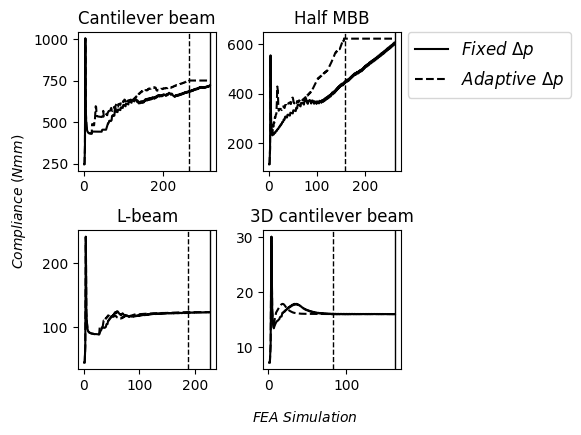
\includegraphics[width=\textwidth]{images/adaptive_csimp/convplots_dec_tol_csimp_03_0001_80_001_ip.png}
    \caption{Convergence plots of Dec-Tol CSIMP using $tol_0 = 0.01$, $tol_{min} = 0.0001$, $V = 0.3$, and $\Delta p = 0.05$ with and without penalty adaptation for the 4 test problems.}
    \label{fig:dec_tol_convplots}
  \end{figure}

  Figure \ref{fig:dec_tol_convplots} shows a typical convergence plot of the decreasing tolerance schemes with and without penalty step adaptation. It is clear that penalty adaptation was successful in many cases in accelerating the convergence of the algorithm for all the test problems, reducing the number of FEA simulations required by an average of 28.8 \%, without significant compromise to C-Obj, $4.1\%$ in the worst case. Finally, Figures \ref{fig:dec_tol_tops} and \ref{fig:dec_tol_tops2} show the final topologies of some of the test instances with and without penalty step adaptation using the decreasing tolerance scheme. For clarity, the binary solution is shown in the 3D case, while the continuous one is shown for the 2D problems.

  \begin{figure}
    \begin{subfigure}{0.45\textwidth}
      \centering
      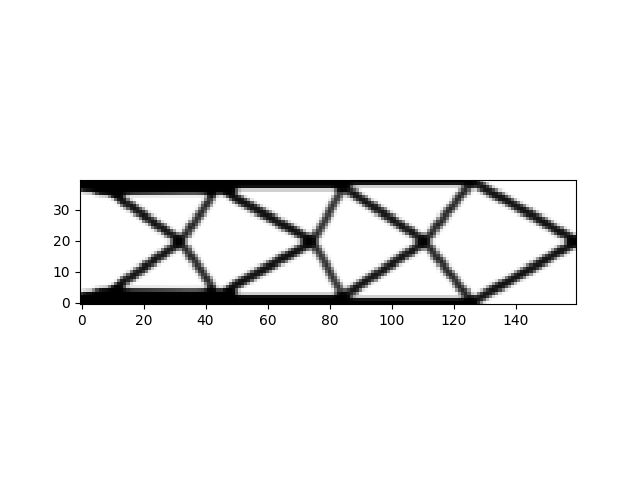
\includegraphics[width=1\textwidth]{images/adaptive_csimp/cantilever_dec_tol_csimp_03_0001_80_false_001_ip.png}
      \caption{Fixed $\Delta p = 0.05$, $V = 0.3$.}
    \end{subfigure} \hfill
    \begin{subfigure}{0.45\textwidth}
      \centering
      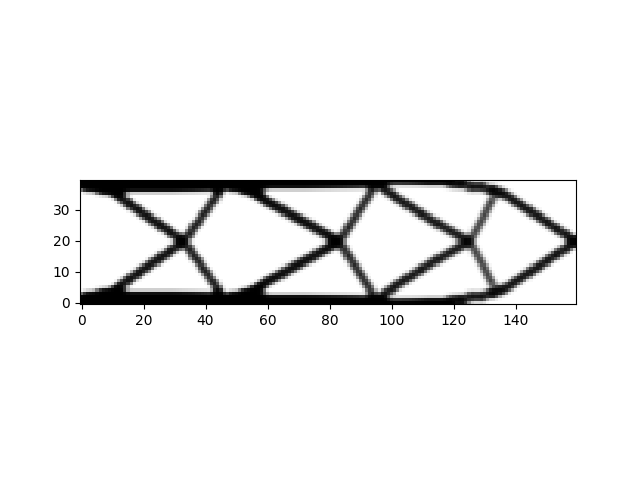
\includegraphics[width=1\textwidth]{images/adaptive_csimp/cantilever_dec_tol_csimp_03_0001_80_true_001_ip.png}
      \caption{Adaptive $\Delta p$, $\Delta p_0 = 0.05$, $V = 0.3$.}
    \end{subfigure}

    \begin{subfigure}{0.45\textwidth}
      \centering
      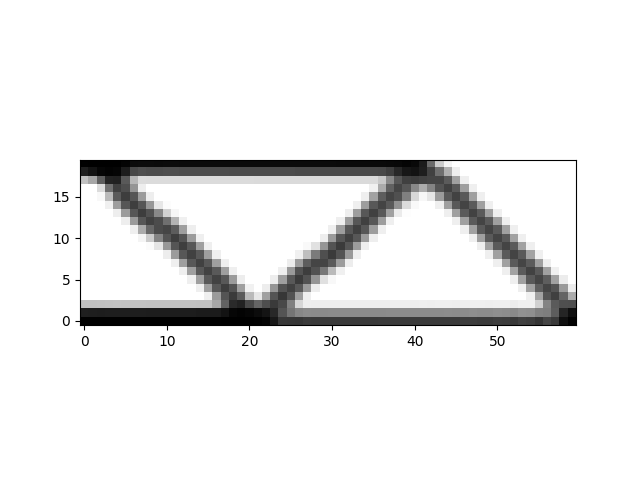
\includegraphics[width=1\textwidth]{images/adaptive_csimp/halfmbb_dec_tol_csimp_03_0001_80_false_001_ip.png}
      \caption{Fixed $\Delta p = 0.05$, $V = 0.3$.}
    \end{subfigure} \hfill
    \begin{subfigure}{0.45\textwidth}
      \centering
      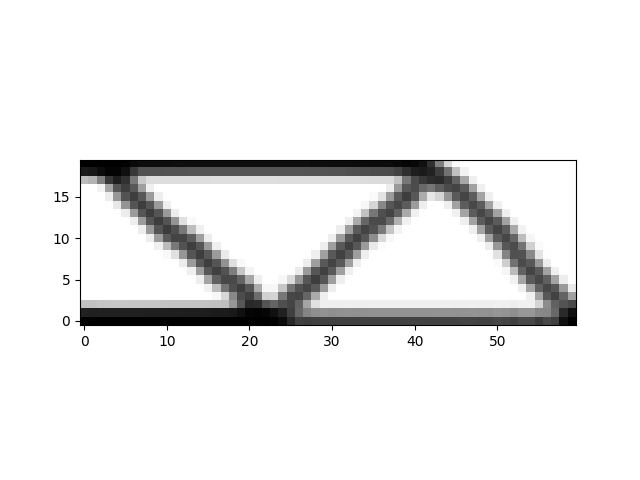
\includegraphics[width=1\textwidth]{images/adaptive_csimp/halfmbb_dec_tol_csimp_03_0001_80_true_001_ip.png}
      \caption{Adaptive $\Delta p$, $\Delta p_0 = 0.05$, $V = 0.3$.}
    \end{subfigure}

    \begin{subfigure}{0.45\textwidth}
      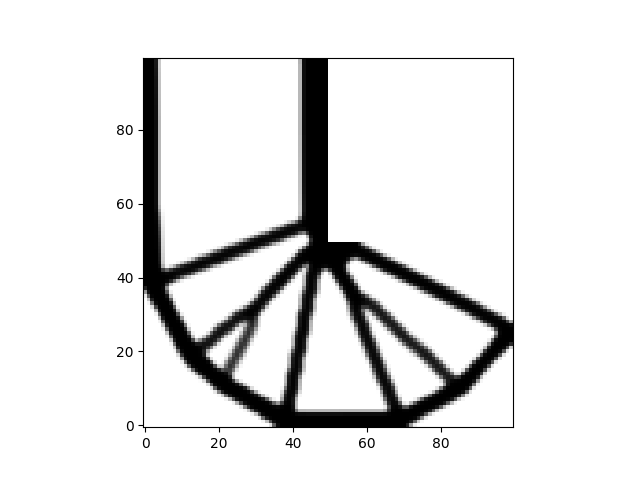
\includegraphics[width=1\textwidth]{images/adaptive_csimp/lbeam_dec_tol_csimp_03_0001_80_false_001_ip.png}
      \caption{Fixed $\Delta p = 0.05$, $V = 0.3$.}
    \end{subfigure} \hfill
    \begin{subfigure}{0.45\textwidth}
      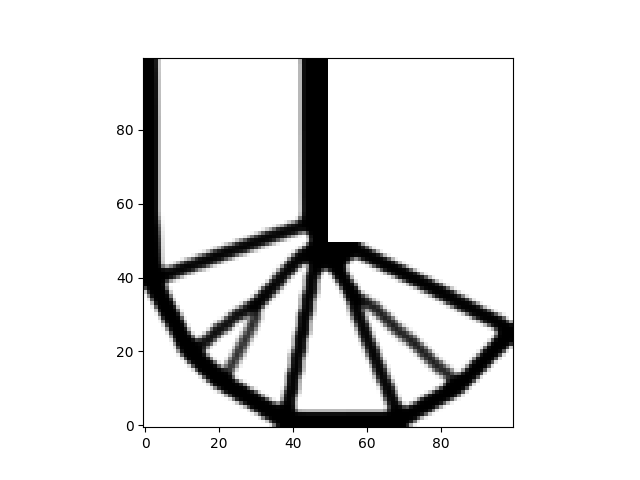
\includegraphics[width=1\textwidth]{images/adaptive_csimp/lbeam_dec_tol_csimp_03_0001_80_true_001_ip.png}
      \caption{Adaptive $\Delta p$, $\Delta p_0 = 0.05$, $V = 0.3$.}
    \end{subfigure}

    \caption{Continuous solutions of Dec-Tol CSIMP with a maximum tolerance of $0.01$ and a minimum tolerance of $0.0001$, with and without $\Delta p$ adaptation.}
    \label{fig:dec_tol_tops}
  \end{figure}

  \begin{figure}
    \begin{subfigure}{0.45\textwidth}
      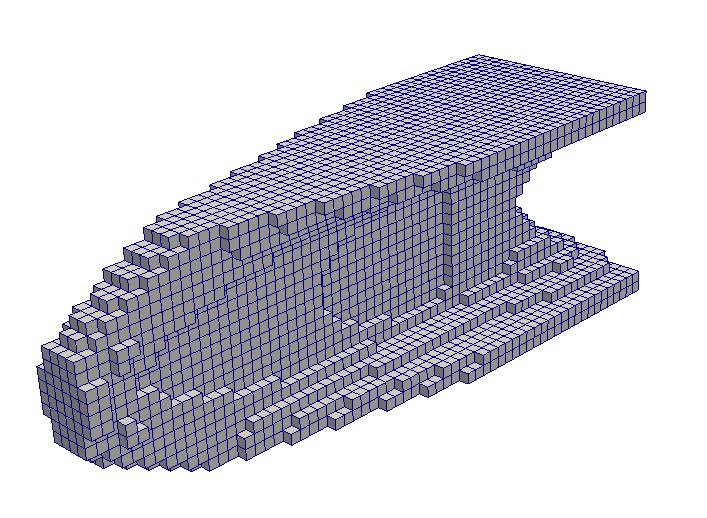
\includegraphics[width=1\textwidth]{images/adaptive_csimp/cantilever3d_false}
      \caption{Fixed $\Delta p = 0.05$, $V = 0.3$.}
    \end{subfigure} \hfill
    \begin{subfigure}{0.45\textwidth}
      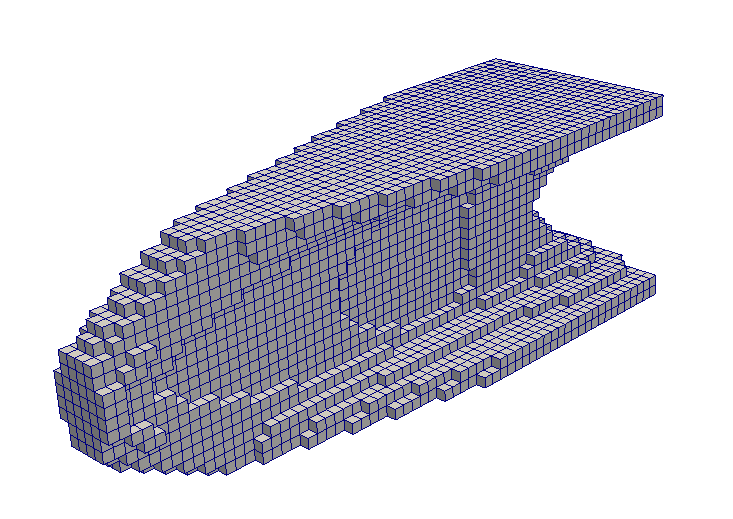
\includegraphics[width=1\textwidth]{images/adaptive_csimp/cantilever3d_true}
      \caption{Adaptive $\Delta p$, $\Delta p_0 = 0.05$, $V = 0.3$.}
    \end{subfigure}

    \caption{Binary solutions of the 3D cantilever beam problem using Dec-Tol CSIMP with a maximum tolerance of $0.01$ and a minimum tolerance of $0.0001$, with and without $\Delta p$ adaptation.}
    \label{fig:dec_tol_tops2}
  \end{figure}

  % Intermediate

  To further highlight that the reduction in the number of FEA simulations due to penalty adaptation is not trivial, Figure \ref{fig:intermediate_solution_lbeam} shows the intermediate solution of Dec-Tol CSIMP without penalty adaptation when solving the L-beam problem in Exp 10, $V = 0.3$, and $\Delta p = 0.05$ after 186 FEA simulations. Dec-Tol CSIMP with penalty adaptation only required 186 FEA simulations to converge for this problem while Dec-Tol CSIMP without penalty adaptation required 226. The intermediate solution, shown in Figure \ref{fig:cont_intermediate_solution_lbeam} is infeasible due to disconnected parts. The compliance of the binary solution is therefore not defined. This is in contrast to Figure \ref{fig:solution_final_lbeam_csimp_true} which shows the solution when using penalty adaptation after the same number of FEA simulations as Figure \ref{fig:intermediate_solution_lbeam}.

  \begin{figure}
    \centering
    \begin{subfigure}[t]{0.45\textwidth}
      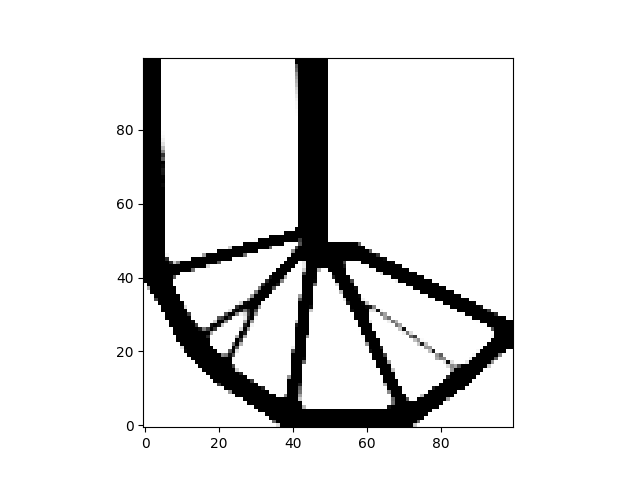
\includegraphics[width=0.9\textwidth]{images/adaptive_csimp/lbeam_dec_tol_csimp_intermediate_03_001_80.png}
      \caption{Continuous intermediate solution.}
      \label{fig:cont_intermediate_solution_lbeam}
    \end{subfigure} \hfill
    \begin{subfigure}[t]{0.45\textwidth}
      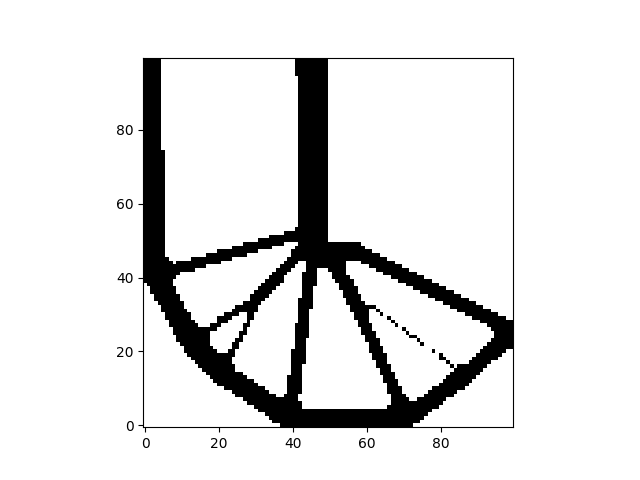
\includegraphics[width=0.9\textwidth]{images/adaptive_csimp/lbeam_dec_tol_csimp_intermediate_binary_03_001_80.png}
      \caption{Projected binary intermediate solution.}
      \label{fig:bin_intermediate_solution_lbeam}
    \end{subfigure}
    \caption{The continuous and projected intermediate solutions of the L-beam problem using Dec-Tol CSIMP without penalty adaptation after 186 FEA simulations using $V = 0.3$, and $\Delta p = 0.05$. CSIMP with penalty adaptation requires only 186 FEA simulations to converge, whereas without penalty adaptation, it takes 226 FEA simulations.}
    \label{fig:intermediate_solution_lbeam}
  \end{figure}

  \begin{figure}
    \centering
    \begin{subfigure}[t]{0.45\textwidth}
      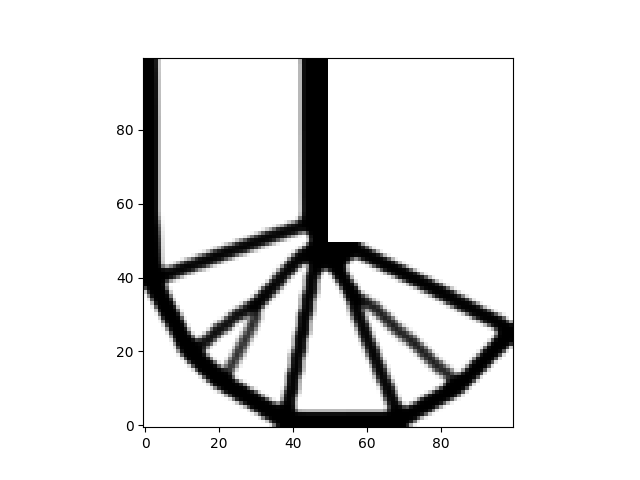
\includegraphics[width=0.9\textwidth]{images/adaptive_csimp/lbeam_dec_tol_csimp_03_0001_80_true_001_ip.png}
      \caption{This is the final continuous solution. The objective value is 123.7.}
      \label{fig:solution_final_lbeam_cont_csimp_true}
    \end{subfigure} \hfill
    \begin{subfigure}[t]{0.45\textwidth}
      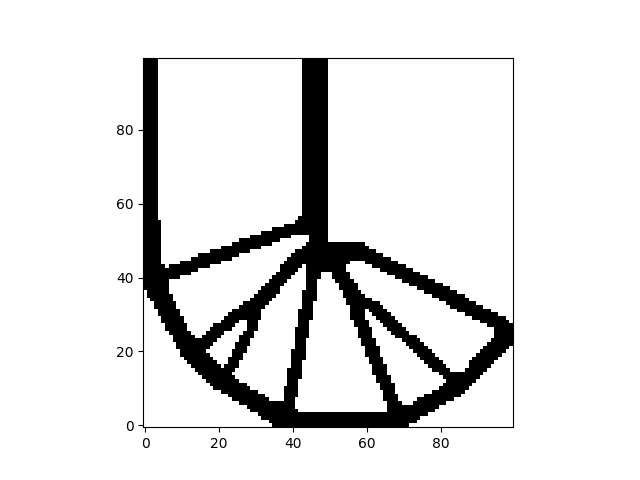
\includegraphics[width=0.9\textwidth]{images/adaptive_csimp/lbeam_dec_tol_csimp_binary_03_0001_80_true.png}
      \caption{This is the projected final solution where $x_e$ is binary for all $e$. The objective value is 104.3.}
      \label{fig:solution_final_lbeam_binary_csimp_true}
    \end{subfigure}
    \caption{The continuous and projected final solutions of the L-beam problem using Dec-Tol CSIMP with penalty adaptation using $V = 0.3$, and $\Delta p = 0.05$. Convergence happened after 186 FEA simulations.}
    \label{fig:solution_final_lbeam_csimp_true}
  \end{figure}

\section{Effect of $x_{min}$} \label{sec:xmin_sens}

  In the vast majority of papers in literature, the value of $x_{min}$ used is 0.001. Some papers seem to penalize the value of $0 \leq x_e \leq 1$ while others seem to penalize the value of $\rho_e = x_e (1 - x_{xmin}) + x_{min}$. In this chapter, the former has been used. The latter has the effect of decreasing the minimum value that $\rho_e$ can take as the penalty increases. While the mentioned reason for using $x_{min} > 0$ in literature is to stop the stiffness matrix $\bm{K}$ from becoming singular, this is not free of limitations. In this section, it will be proven that in the VCCM problem, $x_{min}$ plays the role of a penalty for 2 types of infeasible designs: 1) a design with a force on a node with no element to support it, and 2) a design with rigid body modes on which a non-orthogonal force is applied, i.e. the force has a component along one or more of the rigid body modes. The effect of $x_{min}$ on the number of FEA simulations required to solve the problem will then be presented.

  Let the nodes that have all their elements removed, i.e. $x_e = 0$, be called \textit{shadow nodes}, and let any degree of freedom (dof) of a shadow node be called a \textit{shadow dof}. In the case where $x_{min} = 0$, shadow dofs do not have any non-zero value in their corresponding rows and columns of the stiffness matrix $\bm{K}$. A low $x_{min}$ approximates this without letting $\bm{K}$ become singular. Experiments show that the nodal displacements and compliance of the optimal solutions often reach a finite limit value as $x_{min} \to 0$ for the optimal topologies, with non-zero displacements for the shadow nodes. When $x_{min}$ is 0, $\bm{K}$ becomes rank deficient if a shadow dof exists. Note that: 
  \begin{align}
    \bm{u} = \bm{K}^{-1} \bm{f} = \sum_j \frac{1}{\lambda_j} \bm{v}_j \bm{v}_j^T \bm{f}
  \end{align}
  where $\bm{v}_j$ is the $j^{th}$ eigenvector of $\bm{K}$ and $\lambda_j$ is the corresponding eigenvalue. Additionally, without loss of generality, let the $i^{th}$ dof be a shadow dof that has no Dirichlet boundary condition. It is easy to show that as $x_{min}$ goes to 0, that the span of the eigenspace of $\bm{K}$ associated with the eigenvalue of 0, admits a new basis vector $\bm{e}_i$, where $\bm{e}_i$ is the $i^{th}$ standard basis vector. This is easy to see since the matrix $\bm{K}$'s $i^{th}$ row and column are all zeros, so $\bm{K} \bm{e}_i = 0 \times \bm{e}_i$. Given the limit eigenvector, $\bm{e}_i$, one can also obtain the limit eigenvalue using the Rayleigh quotient $\frac{\bm{e}^T_i \bm{K} \bm{e}_i}{\bm{e}^T_i \bm{e}_i} = K_{ii} = x_{min} \times \sum_e K_{e,ii}$, where $K_{ii}$ is the $i^{th}$ diagonal element of the matrix $\bm{K}$, $\bm{K}_e$ is the extended form of the element stiffness matrix of the element $e$ such that $\bm{K}_e$ is the same size as $\bm{K}$ but only has non-zeros where element $e$'s degrees of freedom are, and $K_{e,ii}$ is $i^{th}$ diagonal element of $\bm{K}_e$. The following relationship therefore holds:
  \begin{align}
    \lim_{x_{min} \to 0} \bm{u} & = \lim_{x_{min} \to 0} \sum_j \frac{1}{\lambda_j} \bm{v}_j \bm{v}_j^T \bm{f} \\ 
    & = \lim_{x_{min} \to 0} \frac{1}{\lambda_i} \bm{v}_i \bm{v}_i^T \bm{f} + \sum_{j \neq i} \frac{1}{\lambda_j} \bm{v}_j \bm{v}_j^T \bm{f} \\
    & = \lim_{x_{min} \to 0} \frac{1}{x_{min} \times \sum_e K_{e,ii}} \bm{e}_i \bm{e}_i^T \bm{f} + \sum_{j \neq i} \frac{1}{\lambda_j} \bm{v}_j \bm{v}_j^T \bm{f}\\
    & = \lim_{x_{min} \to 0} \frac{f_i}{x_{min} \times \sum_e K_{e,ii}} \bm{e}_i + \sum_{j \neq i} \frac{1}{\lambda_j} \bm{v}_j \bm{v}_j^T \bm{f}
  \end{align}
  where $f_i$ is the $i^{th}$ element of the vector $\bm{f}$. Notice that if $f_i = 0$, the limit of the first term will be 0. Whereas, if $f_i \neq 0$, the limit will be $\pm \infty$ depending on the sign of $f_i$. The above derivations give a natural necessary condition for the finiteness of the displacements $\bm{u}$ and the compliance $C$. If the displacements and hence the compliance are to be finite, all shadow degrees of freedom should have no force component corresponding to them. In other words, every force should have at least one element to support it.

  The above condition can be enforced with constraints or it can be enforced by making $x_{min}$ small enough. Let $x_{min}$ be small enough, so we can approximate $\bm{u}$ by its limit term:
  \begin{align}
    \bm{u} & \approx \sum_{i \in I} \frac{f_i}{x_{min} \times \sum_e K_{e,ii}} \bm{e}_i + \sum_{j \notin I} \frac{1}{\lambda_j} \bm{v}_j \bm{v}_j^T \bm{f}
  \end{align}
  where $I$ is the set of shadow dofs. The compliance $C = \bm{f}^T \bm{u}$ can therefore be approximated by:
  \begin{align}
    C & \approx \sum_{i \in I} \frac{f^2_i}{x_{min} \times \sum_e K_{e,ii}} + \sum_{j \notin I} \frac{1}{\lambda_j} (\bm{v}_j^T \bm{f})^2
  \end{align}

  Since $\bm{K}$ is positive semi-definite, $\lambda_j \geq 0 \quad \forall j$. So we can approximately lower bound the compliance $C$ using:
  \begin{align}
    C \gtrapprox \sum_{i \in I} \frac{f^2_i}{x_{min} \times \sum_e K_{e,ii}}
  \end{align}

  Therefore, one can see that a lower $x_{min}$ \textit{penalizes} the compliance of the designs with shadow degrees of freedom corresponding to a force component. This means that if the binary solution projected from the optimal continuous one introduces shadow dofs, then the value of $x_{min}$ may not have been small enough. In other words, a higher $x_{min}$ increases the chances of getting an \textit{optimal} design with a shadow dof where a force component is applied. This is clearly not a feasible design in the exact sense. The above derivations also suggest the possibility of using a weighted compliance term in the objective in classes of topology optimization problems other than VCCM to trigger the penalization effect of $x_{min}$.

  Similar derivations can be followed to show that $x_{min}$ also penalizes a design with rigid body modes. Let $\bm{K}(x_{min})$ be the stiffness matrix of a disconnected binary design for some value of $x_{min}$. Since $\bm{K}$ is positive definite when $x_{min} > 0$, $\bm{u}^T \bm{K} \bm{u} > 0 \quad \forall \bm{u}$. Let $\bm{v}_i$ be the $i^{th}$ rigid body mode of a subset of the elements, e.g. a disconnected piece, when $x_{min} = 0$. Since $\bm{v}_i$ is a rigid body mode, $\bm{v}_i^T \bm{K}(0) \bm{v}_i = 0$. Let $\bm{K} = \bm{K}_{f_i} + \bm{K}_{p_i} + x_{min} \times \bm{K}_{v_i}$ be the decomposition of $\bm{K}$ into free, pinned and void components of the binary design, respectively, with respect to the rigid body mode $\bm{v}_i$. $\bm{K}_{f_i}$ is assembled from the solid elements that the rigid body mode $\bm{v}_i$ moves, $\bm{K}_{p_i}$ is assembled from the remaining solid elements, and $\bm{K}_{v_i}$ is assembled from the void elements. Let $\bm{K}$ have the boundary conditions properly applied, with the Dirichlet dofs having only a positive diagonal term in $\bm{K}$. If such a dof is part of 2 matrices of $\bm{K}_{f_i}$, $\bm{K}_{p_i}$ and $\bm{K}_{v_i}$, half the value can be used in each. Let's first consider the case where the component with the free body mode is disconnected from the pinned component. Since $\bm{v}_i$ is a rigid body mode of the elements making up $\bm{K}_{f_i}$, and the set of dofs of $\bm{K}_{p_i}$ is disjoint from the set of dofs making up $\bm{K}_{f_i}$, $\bm{v}_i^T \bm{K}_{f_i} \bm{v}_i = \bm{v}_i^T \bm{K}_{p_i} \bm{v}_i = 0$. The same holds for the case where the free component is not fully disconnected but hinged on a point, or a line in 3D space, since the dofs of the hinge do not contribute to the rigid body mode. Therefore, $\bm{v}_i^T \bm{K} \bm{v}_i = x_{min} \times \bm{v}_i^T \bm{K}_{v_i} \bm{v}_i$. Assuming $\bm{v}_i$ is a unit vector, $\bm{v}_i^T \bm{K} \bm{v}_i$ is the Rayleigh quotient of the limit eigenvector $\bm{v}_i$ corresponding to a 0 eigenvalue, as $x_{min} \to 0$. Therefore, the following holds:
  \begin{align}
    \lim_{x_{min} \to 0} \bm{u} & = \lim_{x_{min} \to 0} \bm{K}(x_{min})^{-1} \bm{f}\\
    & = \lim_{x_{min} \to 0} \sum_{i \in J} \frac{\bm{v}_i^T \bm{f}}{x_{min} \times \bm{v}_i^T \bm{K}_{v_i} \bm{v}_i} \bm{v}_i + \sum_{j \notin J} \frac{1}{\lambda_j} \bm{v}_j \bm{v}_j^T \bm{f}
  \end{align}
  where $\{\bm{v}_i: i \in J\}$ is the set of rigid body modes at $x_{min} = 0$. Note that the second term above can further be broken down into 2 terms, one for the shadow dofs, and one for the remaining components:
  \begin{align}
    \lim_{x_{min} \to 0} \bm{u} & = \lim_{x_{min} \to 0} \sum_{i \in I} \frac{f_i}{x_{min} \times \sum_e K_{e,ii}} \bm{e}_i + \sum_{i \in J} \frac{\bm{v}_i^T \bm{f}}{x_{min} \times \bm{v}_i^T \bm{K}_{v_i} \bm{v}_i} \bm{v}_i + \sum_{j \notin I, j \notin J} \frac{1}{\lambda_j} \bm{v}_j \bm{v}_j^T \bm{f}
  \end{align}

  The limit compliance can then be written as:
  \begin{align}
    \lim_{x_{min} \to 0} C & = \lim_{x_{min} \to 0} \sum_{i \in I} \frac{f_i^2}{x_{min} \times \sum_e K_{e,ii}} + \sum_{i \in J} \frac{(\bm{v}_i^T \bm{f})^2}{x_{min} \times \bm{v}_i^T \bm{K}_{v_i} \bm{v}_i} + \sum_{j \notin I} \frac{(\bm{v}_j^T \bm{f})^2}{\lambda_j}
  \end{align}

  When $x_{min}$ is small enough that one can use the limit expression to approximate the value of $C$, one can see that $x_{min}$ indeed plays the role of a penalty for any design with a shadow dof $i$ and a force component $f_i \neq 0$, or any design with a rigid body mode on which a non-orthogonal force is applied such that $\bm{v}_i^T \bm{f} \neq 0$.
  \begin{align}
    C \gtrapprox \sum_{i \in I} \frac{f^2_i}{x_{min} \times \sum_e K_{e,ii}} + \sum_{i \in J} \frac{(\bm{v}_i^T \bm{f})^2}{x_{min} \times \bm{v}_i^T \bm{K}_v \bm{v}_i}
  \end{align}

  The experimental results shown in Table \ref{tab:dec_tol_csimp_xmin} indicate that a higher value of $x_{min}$ can lead to faster convergence. This is not surprising since MMA uses first order approximation of the objective and constraints. So if the objective function varies significantly in the neighbourhood of local minima, the first order approximation is likely to cause the solution to jump from one basin of attraction to another during an MMA iteration. However, too high a value can lead to a final design that is infeasible in the exact sense. From the above approximate lower bound expression, one can see that the best choice of $x_{min}$ is very much problem-dependent. This is because the penalization effect of $x_{min}$ is undermined if the norm of $\bm{K}_e$ is increased for all $e$. One way to increase the norm of $\bm{K}_e$ is to use a higher Young's modulus $E$.

  A better way to choose the value of $x_{min}$ is to make sure that $x_{min} = \frac{\epsilon}{\lambda_{max}}$, where $\epsilon$ is a small number and $\lambda_{max}$ is the maximum eigenvalue of the stiffness matrix of the ground mesh. It is simple to show that $\sum_e K_{e,ii}$ and $\bm{v}_i^T \bm{K}_{v_i} \bm{v}_i$ are both less than or equal to $\lambda_{max}$. 

  \begin{proof}
    Let $\lambda_{min}$ and $\lambda_{max}$ be the minimum and maximum eigenvalues of the positive definite matrix $\bm{K}$ at the ground mesh, respectively. It is well known that:
    \begin{align}
      &  0 < \lambda_{min} \leq \frac{\bm{x}^T \bm{K} \bm{x}}{\bm{x}^T \bm{x}} \leq \lambda_{max} \quad \forall \bm{x} \in \mathbb{R}^n
    \end{align}
    where $n$ is the number of degrees of freedom \cite{Golub1996}. This inequality holds for all $\bm{x} \in \mathbb{R}^n$ including the standard basis vector $\bm{e}_i$ corresponding to the $i^{th}$ shadow dof as well as any orthonormal rigid body mode $\bm{v}_i$.
    \begin{align}
      &  0 < \lambda_{min} \leq \bm{e}_i^T \bm{K} \bm{e}_i = \sum_e K_{e,ii} \leq \lambda_{max} \\
      &  0 < \lambda_{min} \leq \bm{v}_i^T \bm{K} \bm{v}_i \leq \lambda_{max}
    \end{align}
    Additionally, since each element stiffness matrix $\bm{K}_e$ is positive semi-definite, $\bm{K}_{f_i}$, $\bm{K}_{p_i}$ and $\bm{K}_{v_i}$ are all positive semi-definite with a non-negative quadratic form. Therefore:
    \begin{align}
      & \bm{v}_i^T \bm{K}_{v_i} \bm{v}_i \leq \bm{v}_i^T \bm{K}_{f_i} \bm{v}_i + \bm{v}_i^T \bm{K}_{p_i} \bm{v}_i + \bm{v}_i^T \bm{K}_{v_i} \bm{v}_i = \bm{v}_i^T \bm{K} \bm{v}_i \leq \lambda_{max}
    \end{align}
    \textit{This completes the proof}.
  \end{proof}

  Let $LB = \sum_{i \in I} \frac{f^2_i}{x_{min} \times \sum_e K_{e,ii}} + \sum_{i \in J} \frac{(\bm{v}_i^T \bm{f})^2}{x_{min} \times \bm{v}_i^T \bm{K}_{v_i} \bm{v}_i}$. If $x_{min} = \frac{\epsilon}{\lambda_{max}}$:
  \begin{align}
    LB & \geq \sum_{i \in I} \frac{f^2_i}{\epsilon} + \sum_{i \in J} \frac{(\bm{v}_i^T \bm{f})^2}{\epsilon} \\
    C & \gtrapprox \frac{1}{\epsilon} \Bigg( \sum_{i \in I} f^2_i + \sum_{i \in J} (\bm{v}_i^T \bm{f})^2 \Bigg)
  \end{align} 
  Therefore, penalization will not be undermined by the scale of $\bm{K}$. Choosing an appropriate value of $\epsilon$ is not an easy task. It needs to be small enough so that designs in the neighbourhood with one of the 2 penalized cases have a worse compliance than other feasible designs, in the exact sense of feasibility. A future research direction can be on efficient ways to choose and adapt the value of $\epsilon$. Figure \ref{fig:high_xmin_solution_cantilever} shows the final continuous design of Dec-Tol CSIMP without penalty adaptation using $x_{min} = 0.01$ and $x_{min} = 0.001$, for volume fraction $V = 0.1$. It is clear that the second infeasibility case is present. Note that unlike $x_{min}$, $\epsilon$ is not a dimensionless quantity. $\epsilon$ has the same unit as the elements of the stiffness matrix, i.e. $N/mm$.

  \begin{table}
\centering
\tabcolsep=0.09cm
% table caption is above the table
\caption{This table shows the effect of increasing $x_{min}$ on CSIMP with decreasing tolerance and a fixed penalty step. The table shows the results of the experiments studying the effect of increasing $x_{min}$: 1) the number of FEA simulations (Sims) required by CSIMP, 2) the final objective of the continuous NLP at $p = 5$ (C-Obj), 3) the objective value of the rounded discrete solution (D-Obj), and 4) the percentage of fractionness (\% frac). The parameters of each experiment are described in Table \ref{tab:exp_params2}.}
\label{tab:dec_tol_csimp_xmin}
\begin{tabular}{|l|l|l|l|l||l|l|}
\hline\noalign{\smallskip}
Exp & \multicolumn{3}{c||}{\textbf{$x_{min} = 0.001$}} & \multicolumn{3}{c|}{\textbf{\% Increase - $x_{min} = 0.01$}} \\
\noalign{\smallskip}\hline\noalign{\smallskip}
& \textbf{Sims} & \textbf{C-Obj / D-Obj} & \textbf{\% frac} & \textbf{Sims} & \textbf{C-Obj / D-Obj} & \textbf{\% frac}\\
\hline
1 & 185 & 814.2/581.6 & 17.3 & -23.8 & -16.4/-4.2 & -18.5 \\ 
\hline
2 &  316 & 720.4/553.1 & 14.0 & -29.7 & -5.9/2.8 & 0.0 \\ 
\hline
3 &  139 & 375.0/342.3 & 11.5 & -15.1 & -3.3/-1.3 & -12.2 \\ 
\hline
4 &  236 & 367.3/338.9 & 9.8 & -23.3 & -1.5/-0.1 & 2.0 \\ 
\hline
\hline
5 & 130 & 619.6/293.9 & 24.6 & -7.7 & -13.9/14.0 & -0.8 \\ 
\hline
6 & 260 & 606.5/292.8 & 24.3 & -21.2 & -12.4/9.6 & 0.0 \\ 
\hline
7 & 130 & 219.5/175.3 & 18.1 & -7.7 & -2.9/1.0 & -0.6 \\ 
\hline
8 & 211 & 218.8/175.1 & 17.9 & -6.6 & -2.6/1.1 & 1.1 \\ 
\hline
\hline
9 & 153 & 121.5/103.4 & 9.0 & -20.9 & -3.0/1.3 & 1.1 \\ 
\hline
10 & 226 & 123.5/104.1 & 9.6 & -14.6 & -4.7/0.5 & -5.2 \\ 
\hline
11 & 142 & 69.8/65.6 & 6.8 & -26.8 & -0.9/0.5 & -4.4 \\ 
\hline
12 & 192 & 69.9/65.7 & 6.8 & -12.0 & -1.1/0.2 & -2.9 \\ 
\hline
\hline
13 & 97 & 16.1/13.1 & 10.1 & -1.0 & -1.9/0.0 & 2.0 \\ 
\hline
14 & 161 & 16.0/13.1 & 10.1 & 0.0 & -1.2/0.0 & 1.0 \\ 
\hline
15 & 97 & 10.2/9.3 & 10.9 & 0.0 & -1.0/0.0 & -0.9 \\ 
\hline
16 & 161 & 10.2/9.3 & 11.0 & 0.0 & -1.0/0.0 & -0.9 \\ 
\hline
\noalign{\smallskip}\hline
\end{tabular}
\end{table}


  \begin{figure}[H]
    \centering
    \begin{subfigure}{0.45\textwidth}
      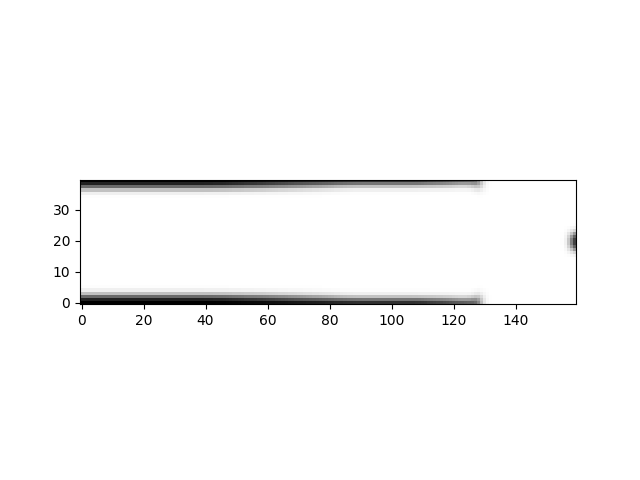
\includegraphics[width=0.9\textwidth]{./images/adaptive_csimp/cantilever_dec_tol_csimp_01_0001_80_false_01_ip.png}
      \caption{$x_{min} = 0.01$.}
    \end{subfigure} \hfill
    \begin{subfigure}{0.45\textwidth}
      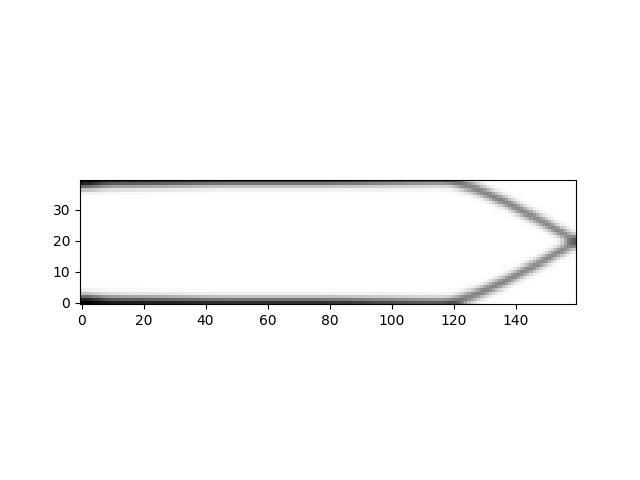
\includegraphics[width=0.9\textwidth]{./images/adaptive_csimp/cantilever_dec_tol_csimp_01_0001_80_false_001_ip.png}
      \caption{$x_{min} = 0.001$.}
    \end{subfigure}
    \caption{2D cantilever problem using Dec-Tol CSIMP without penalty adaptation using $V = 0.1$, $\Delta p = 0.05$.}
    \label{fig:high_xmin_solution_cantilever}
  \end{figure}

\section{Conclusion} \label{sec:conclusion}

  In this chapter, a penalty step adaptation technique for the continuation SIMP algorithm was proposed and tested. Four common test problems from literature, three 2D and one 3D, were used to test the efficacy of the penalty adaptation with different parameter settings. The main factors affecting the efficacy of the penalty adaptation in the CSIMP algorithm in reducing the number of FEA simulations needed to converge to the final solution were identified. The experimental results demonstrate a significant reduction in the number of FEA simulations required to reach the optimal solution in the decreasing tolerance continuation SIMP algorithm, with exponentially decaying tolerance, with little to no detriment in the objective value and the other metrics used. Finally, a mathematical and experimental treatment of the effect of $x_{min}$ on the convergence of the SIMP algorithm was given with some recommendations for choosing a suitable $x_{min}$.


\clearpage
\newpage

	\let\cleardoublepage\clearpage

	\begin{titlepage}\centering
\vspace*{\fill}

\chapter{Exact compliance-based optimization with finitely many loading scenarios}\thispagestyle{EmptyHeader}
\label{chp:3}

\begin{tcolorbox}
This work is accepted for publication in the Journal of Structural and Multidisciplinary Optimization. The accepted manuscript can be found on arXiv (https://arxiv.org/abs/2103.04594). The paper is titled: "Robust and stochastic compliance-based topology optimization with finitely many loading scenarios"  \citep{tarek2021robust}
\end{tcolorbox}

\vspace*{\fill}
\end{titlepage}

\newpage

\section{Introduction}

Handling load uncertainty naively in topology optimization can prohibitively increase the computational cost of topology optimization. In this chapter, efficient methods to handle load uncertainty will be reviewed and novel ones will be proposed for compliance-based topology optimization.

\section{Literature review}

  \subsection{Mean compliance minimization}

    A number of works in literature tackled the problem of load uncertainty in compliance minimization problems. A general scheme for mean compliance minimization subject to uncertain load components with arbitrary covariance was proposed by \cite{Guest2008}. Guest et al. also considered uncertain load locations by treating the loaded nodes' locations as random and hence the stiffness matrix. Guest et al. then derived an approximately equivalent load distribution that would result in the same mean compliance while deterministically using the mean stiffness matrix. Mean compliance minimization subject to uncertainty of concentrated load magnitude and direction was studied by \cite{Dunning2011}. Dunning et al. derived efficient formulations for the mean compliance subject to such uncertainties, where the number of linear systems to be solved scales linearly with the number of independent random variables. This assumes that the distribution of the forces' magnitudes and rotations are known and independent. A similar formulation was then derived by \cite{Zhao2014} which requires fewer linear system solves per independent random variable. Zhao et al. also demonstrated how the same approach can handle distributed load uncertainty, modeled as a stochastic field, using Karhunen-Loeve (K-L) expansion. The main limitation of the K-L expansion method in practice is having to define and commit to a covariance kernel function. Additionally, the more local the covariance is, the higher the number of terms required in the K-L expansion to accurately describe the random field. The number of linear system solves required to compute the mean compliance scales with the number of terms in the K-L expansion.

    \cite{Zhang2017a} proposed an efficient way to compute the mean compliance for finitely many load scenarios with no assumptions about the nature of randomness. This can be used in data-driven design where the loading scenarios are many, and for which data has been collected. Alternatively, loading scenarios may be sampled from the distributions assumed if sufficiently low dimensional. Zhang et al. developed a randomized algorithm inspired by Hutchinson's trace estimator \cite{Hutchinson1990} to minimize the mean compliance: $\frac{1}{N} \sum_i^N \bm{f}^T_i \bm{K}^{-1} \bm{f}_i$, leading to significant computational savings compared to the naive approach. The algorithm can be trivially modified to handle weighted mean compliance which can be used in cases where the number of random variables are many following the approach by \cite{Zhao2014} or when the number of terms of the K-L expansion is high. The main limitation of this approach is that it can only be used to minimize the mean compliance which is not risk-averse since the compliance can be very high for some probable load scenarios. Finally, \cite{Liu2018a} solved the mean compliance minimization problem under a volume constraint subject to load uncertainty modeled using the fuzzy set theoretic cloud model for describing uncertainty.

  \subsection{Risk-averse compliance minimization}

    Beside mean compliance minimization, some authors also studied risk-averse compliance minimization by considering the weighted sum of the mean and variance, the weighted sum of the mean and standard deviation, as well as other risk measures. \cite{Dunning2013} derived an efficient formulation for the variance of the compliance subject to uncertainty in the load magnitude. This was used to minimize a weighted sum of the mean and variance of the compliance. The main limitation of this approach is that it cannot handle random load directions and that the distributions for the load magnitudes are assumed to be known and independent. \cite{Zhao2014b} minimized the weighted sum of the mean and standard deviation of the compliance by deriving an efficient formulation for the calculation of the mean and standard deviation of the compliance and their gradients under uncertain loading modeled as a random field. Zhao et al. used K-L expansion to quantify and describe the randomness using a few random variables, and used Monte Carlo simulation to calculate the fourth moment of those random variables which is required for the efficient computation of the standard deviation of the compliance.

    \cite{Chen2010} used the level-set method to minimize the weighted sum of the mean compliance and its variance subject to uncertainty in the load and material properties. Chen et al. assumed the load and material properties to be random fields and used K-L expansion to reduce their dimensionality. The authors then used Gaussian quadrature sampling to generate a representative set of scenarios to formulate the mean and variance of the compliance. \cite{Martinez-Frutos2016} used a similar uncertainty quantification approach to develop a multi-GPU density-based topology optimization framework for the large-scale minimization of the weighted sum of the mean compliance and its variance subject to load uncertainty only. However, Martinez-Frutos et al. used sparse grid sampling instead of Gaussian quadrature. Similarly, \cite{Cuellar2018} used K-L expansion for uncertainty quantification and Gaussian quadrature for sampling, and combined them with the non-intrusive polynomial chaos expansion (PCE) method to provide more accurate estimators for the mean and standard deviation of the compliance and their gradients. \cite{Martinez-Frutos2018} also used K-L expansion and the non-intrusive PCE with sparse grid sampling for the quantification and propagation of the uncertainty in the load and material properties. However, Martinez-Frutos et al. minimized a different compliance risk measure called the \textit{excess probability}, which is the probability that the compliance exceeds a certain threshold value. Note that in all the works above which use K-L expansion and sampling-based uncertainty propagation, the number of linear system solves can be made independent from the number of sampling points given the linearity assumption of the displacement as a function of the load exploited by \cite{Zhao2014b} in their derivation, even though in some of the works this property was not exploited. The number of linear system solves can therefore be assumed to be equal to the number of terms in the K-L expansion only, not the sampling points. 

    Also in risk-averse topology optimization, \cite{Garcia-Lopez2013} used multi-objective evolutionary optimization to optimize the mean and variance of the compliance and obtain the Pareto front of the two objectives. Garcia-Lopez et al. used a sampling method for uncertainty propagation inspired from Taguchi's method for the design of experiments. In this case, the number of linear system solves is equal to the number of sampling points. That beside the use of an evolutionary algorithm which requires many evaluations of the mean and variance of the compliance make the computational cost of this approach extremely high even for medium-sized problems. Finally, \cite{Kriegesmann2019} used FOSM instead of sampling to efficiently propagate the uncertainty estimating the mean and standard deviation of the compliance and their gradients from the means and standard deviations of the loads. A weighted sum of the mean and standard deviation of the compliance was then minimized. This approach assumes that the compliance is a linear function of the random load centered at the MPP load, an assumption which leads to a prediction error in the mean and standard deviation of the compliance. 

  \subsection{Probabilistic constraints and reliability-based topology optimization}

    \cite{Keshavarzzadeh2017} solved the problem of volume minimization subject to a probabilistic compliance constraint. In one case, the authors constrained the mean compliance plus a multiple of its standard deviation which is equivalent to a reliability constraint assuming the compliance is normally distributed. In another, a reliability constraint was used such that the probability that the compliance exceeds a threshold value is constrained. Keshavarzzadeh et al. used the non-intrusive PCE and regularized Heaviside function to approximate the compliance reliability constraint and its gradient. PCE was also used to estimate the mean and standard deviation of the compliance and their gradients.

    Beside sampling-based uncertainty propagation, RBDO offers a number of techniques for efficient, approximate uncertainty propagation which can be used for handling probabilistic constraints involving compliance or otherwise. \cite{Kharmanda2002,Kharmanda2004} proposed the use of RBDO for topology optimization, also known as reliability-based topology optimization (RBTO), to handle probabilistic constraints due to random loads, geometry and material properties. \cite{Jung2004} used FORM's PMA with SIMP topology optimization method to solve a volume minimization problem with a reliability constraint for geometrically nonlinear structures. The works by Kharmanda et al. and Jung et al. inspired other works such as \cite{Kim2006} who used FORM's RIA and PMA with SIMP to solve volume minimization problems with reliability constraints on the displacement and natural frequency of the structure under loading, material and geometry uncertainties. Another group, \cite{Kim2007,Kim2008}, later used RIA and PMA together with evolutionary structural optimization (ESO) \citep{YM1992,XY1998,Huang2010a} to solve volume minimization problems with a reliability constraint subject to a random load and Young's modulus. \cite{Ouyang2008} used FORM's RIA with the level-set method to solve a compliance minimization problem with a reliability constraint subject to uncertainty in the load and geometry of the ground mesh. 

    \cite{Silva2010} proposed the use of an efficiently obtainable approximate MPP to avoid the need for solving the reliability or inverse reliability problems in every design iteration of RIA or PMA, respectively. Silva et al. and later \cite{Nguyen2011} also considered system reliability-based topology optimization where an aggregated system failure probability is considered instead of component failure probabilities and component limit state functions. \cite{Zhao2016} presented a comparison of a number of RBTO approaches to solve a few topology optimization problems including one with a compliance reliability constraint under stochastic load and Young's modulus. \cite{Jalalpour2016} developed a bi-directional ESO (BESO) \citep{YM1992,XY1998,Huang2010a} algorithm for handling reliability constraints with displacement limit state functions and a finite number of probable loading scenarios in linearly elastic structures. Finally, \cite{Yin2018} proposed an alternative RBTO approach using fuzzy set theory to describe the uncertainty.

  \subsection{Maximum compliance constraint}

    Beside the stochastic and risk-averse topology optimization presented above, a number of works also studied maximum compliance minimization and maximum compliance constrained problems under uncertain loading conditions, where the former can be formulated using the latter as shown earlier. In these papers, no probability distribution is assumed for the uncertain load and therefore they fall under the category of RO. Most of the work on handling non-probabilistic uncertainty in loads assumed that the loads lie in continuous sets. \cite{Brittain2012} for example assumed that the load vector has a fixed norm but arbitrary direction. Brittain et al. used a bi-level min-max optimization approach minimizing the objective with respect to the topology variables in the upper level problem, and maximizing with respect to the load in the lower level problem. However, an efficient algorithm was derived for the lower level maximization problem based on the KKT optimality conditions for the objective and the load's fixed-norm constraint. \cite{Holmberg2015} proposed a nonlinear semidefinite formulation to solve the maximum compliance minimization problem under non-probabilistic load uncertainty, assuming the uncertain load lies in a hyper-ellipsoid uncertainty set:
    \begin{align}
      & \bm{f} = \bm{f}_0 + \bm{Q} \bm{r} \\
      & ||\bm{r}|| \leq 1
    \end{align}
    where $\bm{f}_0$ is the fixed component of the load vector and the columns of $\bm{Q}$ are the axes of the uncertainty hyper-ellipsoid. The same authors, \cite{Thore2017}, later generalized their approach from \cite{Holmberg2015} to handle maximum compliance and maximum stress constraints under the same assumption on the load vector. Similarly, \cite{Liu2018} proposed a bi-level formulation for handling multiple independent loads, each of which lies in a hyper-ellipsoidal uncertainty set. Liu et al. developed an efficient lower level algorithm by solving the Wolfe dual problem. The Wolfe dual problem of the lower level problem is a maximum generalized eigenvalue minimization problem which was solved using an iterative procedure. The multi-ellipsoidal uncertainty set generalizes the interval as well as the spherical uncertainty sets.

    A number of papers were also published on non-probabilistic reliability-based topology optimization (NRBTO) where new reliability indexes and performance measures are defined for various types of continuous uncertainty sets. While some of these works did not solve problems with maximum compliance constraints, but the same techniques can be applied to handle maximum compliance constraints. \cite{Luo2009} proposed a reliability index and performance measure for handling non-probabilistic uncertainty where the uncertain variables lie in a multi-ellipsoid model. Another reliability index for ellipsoidal uncertainty was then proposed by \cite{Wang2018a}. \cite{Wang2017,Wang2019a} proposed another reliability index for handling interval uncertainty sets using interval arithmetic. \cite{Zheng2018a} proposed a reliability index and performance function for uncertain variables in multidimensional parallelepiped convex sets. Another reliability index for mixed interval and ellipsoidal uncertainty was also developed by \cite{Wang2019b}.

    The rest of this chapter is organized as follows. The proposed approaches for handling load uncertainty in continuum compliance problems in the form of a large, finite number of loading scenarios are detailed in sections \ref{sec:proposed_mean}, \ref{sec:proposed_risk} and \ref{sec:proposed_max}. The experiments used and the implementations are then described in section \ref{sec:exp_impl}. Finally, the results are presented and discussed in section \ref{sec:results} before concluding in section \ref{sec:conclusion}.

\section{Compliance sample mean and its gradient} \label{sec:proposed_mean}

  \subsection{Naive approach}

    The compliance sample mean for a finite number $L$ of loading scenarios is $\mu_C = \frac{1}{L} \sum_{i=1}^L \bm{f}_i^T \bm{K}^{-1} \bm{f}_i$ where $\bm{f}_i$ is the $i^{th}$ load scenario, $\bm{K}$ is the stiffness matrix of the design and $\bm{F}$ is the matrix whose columns are the individual loading scenarios $\bm{f}_i$. The direct naive approach is to solve for $\bm{K}^{-1} \bm{f}_i$ for all $i$ and calculate the mean compliance using the above formula. This method is not efficient since it requires $L$ linear system solves plus some additional work to compute the mean with a time complexity of $O(L \times n_{dofs})$, where $n_{dofs}$ is the number of degrees of freedom in the design. When $\bm{F}$ is sparse with only a few $n_{loaded}$ degrees of freedom that are loaded, the complexity of the remaining work to compute the mean compliance $\frac{1}{L} \sum_{i=1}^L \bm{f}_i^T \bm{u}_i$ becomes $O(L \times n_{loaded})$. Even though the factorization of $\bm{K}^{-1}$ can be reused to solve for the $L$ linear systems, if $L$ is close to $n_{dofs}$, the complexity of solving for so many linear systems will be similar to that of the factorization, thus significantly adding to the running time. When using an iterative algorithm to solve for $\bm{K}^{-1}\bm{f}_i$, a good, but expensively formed, preconditioner such as the algebraic multi-grid preconditioner can be similarly reused. In general, significantly reducing the number of linear systems to solve is advantageous in practice even if, as theory may show, the running time is dominated by the initial linear system solve.

    Let the Jacobian of $\bm{\rho}(\bm{x})$ be $\nabla_{\bm{x}} \bm{\rho}(\bm{x})$. Let $\bm{u}_i$ be the displacement response due to load $\bm{f}_i$ and $C_i$ be the compliance $\bm{f}_i^T \bm{u}_i$. The stiffness matrix $\bm{K}$ is typically defined as: $\bm{K} = \sum_e \rho_e \bm{K}_e$. The partial derivative of the compliance $C_i$ with respect to $\rho_e$ is given by $\frac{\partial C_i}{\partial \rho_e} = -\bm{u}_i^T \bm{K}_e \bm{u}_i$. The gradient of $C_i$ with respect to the decision vector $\bm{x}$ is therefore given by: $\nabla_{\bm{x}} C_i(\bm{x}) = \nabla_{\bm{x}} \bm{\rho}(\bm{x})^T \nabla_{\bm{\rho}} C_i(\bm{\rho}(\bm{x}))$ where $\nabla_{\bm{\rho}} C_i(\bm{\rho}(\bm{x}))$ is the gradient of $C_i$ with respect to $\bm{\rho}$ at $\bm{\rho}(\bm{x})$. The gradient of the mean compliance $\mu_C$ is therefore given by $\nabla_{\bm{x}} \mu_C(\bm{x}) = \frac{1}{L} \sum_{i=1}^L \nabla_{\bm{x}} \bm{\rho}(\bm{x})^T \nabla_{\bm{\rho}} C_i(\bm{\rho}(\bm{x}))$. The additional complexity of computing the mean compliance and its gradient with respect to $\bm{\rho}$ is $O(n_E \times L)$. Note that the Jacobian of $\bm{\rho}(\bm{x})$ does not need to be formed explicitly to compute the gradient above, so long as there is a way to pre-multiply the Jacobian's transpose by a vector. The problem with the naive approach is it requires many linear system solves and so doesn't scale well to many loading scenarios.

  \subsection{Singular value decomposition}

    Less naively, one can first attempt to find the singular value decomposition (SVD) of $\bm{F}$. Let the compact SVD of the matrix $\bm{F}$ be $\bm{F} = \bm{U} \bm{S} \bm{V}^T$, where the number of non-zero singular values is $n_s$, $\bm{S}$ is the diagonal matrix of singular values, $\bm{U}$ is a $n_{dofs} \times n_s$ matrix with orthonormal columns, and $\bm{V}$ is $L \times n_s$ matrix with orthonormal columns. Given the SVD, the mean compliance can be written as: $\mu_C = \frac{1}{L} \sum_{i=1}^L \bm{f}_i^T \bm{K}^{-1} \bm{f}_i = \frac{1}{L} tr(\bm{F}^T \bm{K}^{-1} \bm{F})$. This can be further simplified:
    \begin{align}
     \frac{1}{L} tr(\bm{F}^T \bm{K}^{-1} \bm{F}) & = \frac{1}{L} tr(\bm{V} \bm{S} \bm{U}^T \bm{K}^{-1} \bm{U} \bm{S} \bm{V}^T) \\
     & = \frac{1}{L} tr(\bm{S} \bm{U}^T \bm{K}^{-1} \bm{U} \bm{S}) \\
     & = \frac{1}{L} \sum_{i=1}^{n_s} \bm{S}[i,i]^2 \times \bm{U}[:,i]^T \bm{K}^{-1} \bm{U}[:,i]
    \end{align}
    This method requires only $n_s$ linear system solves and an SVD. $n_s$ will be small if the loads in $\bm{F}$ are highly correlated or if only a few degrees of freedom are loaded, i.e. the loads are sparse. Let $n_{loaded}$ be the few loaded degrees of freedom. It is possible to prove in this case that the number of singular values $n_s \leq n_{loaded}$. The computational time complexity of computing the SVD of $\bm{F}$ in the dense case is $O(min(L, n_{dofs})^2 max(L, n_{dofs}))$, while in the sparse case it is only $O(n_{loaded}^2 L)$. If $n_{loaded}$ is a small constant, finding the SVD will be very efficient. Additionally, when only $n_{loaded}$ degrees of freedom are loaded in $\bm{F}$, only the same degrees of freedom will be non-zero in $\bm{U}$, therefore $\bm{U}$ will also be sparse. Other than the complexity of SVD, the additional work to compute the mean compliance has a computational time complexity of $O(n_s \times n_{dofs})$ when $\bm{F}$ (and $\bm{U}$) are dense, and $O(n_s \times n_{loaded})$ when $\bm{F}$ (and $\bm{U}$) are sparse.

    Given the efficient formula for the mean compliance and using the derivative rule of the inverse quadratic from appendix section \ref{app1}, the partial $\frac{\partial \mu_C}{\partial \rho_e}$ is given by: \\ $-\frac{1}{L} \sum_{i=1}^{n_s} \bm{S}[i,i]^2 (\bm{K}^{-1}\bm{U})[:,i]^T \bm{K}_e (\bm{K}^{-1}\bm{U})[:,i]$. The time complexity of computing this assuming we already computed $\bm{K}^{-1} \bm{U}$ is $O(n_s \times n_E)$. 

  \begin{table*}[h!]
   \centering
   \caption{Summary of the computational cost of the algorithms discussed to calculate the mean compliance and its gradient. \#Lin is the number of linear system solves required.}
   \begin{tabular}{| m{1.7cm} | m{0.7cm} | m{1.0cm} | m{4cm} | m{4cm}|} 
    \hline
    \multirow{2}{3em}{Method} & \multirow{2}{2em}{\#Lin} & \multirow{2}{2em}{SVD?} & \multicolumn{2}{c|}{Time complexity of additional work} \\\cline{4-5}
    & & & Dense & Sparse \\
    \hline
    \hline
    Exact-Naive & \(L\) & \xmark & \(O(L \times (n_{dofs} + n_E))\) & \(O(L \times (n_{loaded} + n_E))\) \\
    \hline
    Exact-SVD & \(n_s\) & \cmark & \(O(n_s \times (n_{dofs} + n_E))\) & \(O(n_s \times (n_{loaded} + n_E))\) \\
    \hline
   \end{tabular}
   \label{tab:perf_mean}
  \end{table*}

\section{Scalar-valued function of load compliances and its gradient} \label{sec:proposed_risk}

  In this section, the above approach for computing the sample mean compliance will be generalized to handle the sample variance and standard deviations. The sample variance of the compliance $C$ is given by $\sigma_C^2 = \frac{1}{L-1} \sum_{i=1}^L (C_i - \mu_C)^2$. The sample standard deviation $\sigma_C$ is the square root of the variance. Let $\bm{C}$ be the vector of compliances $C_i$, one for each load scenario. In vector form, $\sigma_C^2 = \frac{1}{L-1} (\bm{C} - \mu_C \bm{1})^T (\bm{C} - \mu_C \bm{1})$. $\bm{C} = diag(\bm{A})$ is the diagonal of the matrix $\bm{A} = \bm{F}^T \bm{K}^{-1} \bm{F}$.

  \subsection{Naive approach}

    If one can compute the vector of load compliances $\bm{C}$, computing the variance and standard deviation is trivial. This approach requires $L$ linear system solves which can be computationally prohibitive if $L$ is large. Other than the linear system solves, the remaining work of computing $C_i = \bm{f}_i^T \bm{u}_i$ for all $i$ has a complexity of $O(L \times n_{dofs})$ when $\bm{F}$ is dense and $O(L \times n_{loaded})$ when $\bm{F}$ is sparse with only $n_{loaded}$ loaded degrees of freedom. In order to compute the vector $\bm{C}$ exactly, one needs to compute $\bm{u}_i = \bm{K}^{-1} \bm{f}_i$ for all $i$. These can further be used to compute the gradients of the load compliances $C_i$ which can be combined to form the Jacobian $\nabla_{\bm{\rho}} \bm{C}$. Assuming $\bm{u}_i$ is cached for all $i$, the time complexity of computing the Jacobian using $\frac{\partial C_i}{\partial \rho_e} = -\bm{u}_i^T \bm{K}_e \bm{u}_i$ is $O(n_E \times L)$.

    However, when interested in the gradient of a scalar-valued function $f$ of $\bm{C}$, there is no need to form the full Jacobian $\nabla_{\bm{x}} \bm{C}(\bm{x})$. It suffices to define an operator to pre-multiply an arbitrary vector $\bm{w}$ by $\nabla_{\bm{x}} \bm{C}(\bm{x})^T$. Using the chain rule, the gradient of $f$ with respect to $\bm{x}$ is given by $\nabla_{\bm{x}} f(\bm{C}(\bm{x})) = \nabla_{\bm{x}} \bm{C}(\bm{x})^T \nabla_{\bm{C}} f(\bm{C}(\bm{x}))$. This operator is equivalent to attempting to find the gradient of the weighted sum of $\bm{C}$, $\bm{w}^T \bm{C}$, where $\bm{w}$ is the constant vector of weights. In the case of a general scalar-valued function $f$, $\bm{w}$ would be $\nabla_{\bm{C}} f(\bm{C}(\bm{x}))$ and is treated as a constant. In the case of the variance, $f(\bm{C}) = \sigma_C^2 = \frac{1}{L-1} (\bm{C} - \mu_C \bm{1})^T (\bm{C} - \mu_C \bm{1})$, therefore $\bm{w} = \nabla_{\bm{C}} f(\bm{C}(\bm{x})) = \frac{2}{L-1} (\bm{C} - \mu_C \bm{1})$. And in the case of the standard deviation $\sigma_C$, $\bm{w} = \frac{1}{(L-1)\sigma_C} (\bm{C} - \mu_C \bm{1})$. This means that computing $\bm{C}$ is required to form $\bm{w}$.

    By caching $\bm{u}_i = \bm{K}^{-1}\bm{f}_i$ for all $i$ when computing $\bm{C}$, one can find the $e^{th}$ element of $\nabla_{\bm{x}} \bm{C}(\bm{x})^T \bm{w}$ using $\sum_{i=1}^L -w_i \bm{u}_i^T \bm{K}_e \bm{u}_i$, where $w_i$ is $i^{th}$ element of $\bm{w}$. Computing $\bm{u}_i^T \bm{K}_e \bm{u}_i$ requires constant time complexity, therefore the additional time complexity of computing $\nabla_{\bm{x}} \bm{C}(\bm{x})^T \bm{w}$ after computing $\bm{C}$ with the direct method is $O(L \times n_E)$. In this case, this is the same complexity as forming the Jacobian first and then multiplying, but in the next algorithms, it will be different.

  \subsection{Singular value decomposition}

    Much like in the mean compliance calculation, the SVD of $\bm{F}$ can be computed to find $C_i$ for all $i$ more efficiently from $\bm{K}^{-1} \bm{U} \bm{S}$. The number of linear system solves required to compute $\bm{K}^{-1} \bm{U} \bm{S}$ is $n_s$, the number of singular values of $\bm{F}$. The computational cost of computing $C_i = \bm{f}_i^T \bm{u}_i = \bm{f}_i^T (\bm{K}^{-1} \bm{U} \bm{S}) V^T[:,i]$ for all $i$ using $\bm{K}^{-1} \bm{U} \bm{S}$ and $\bm{V}$ is $O(L \times n_s \times n_{dofs})$ when $\bm{F}$ is dense and $O(L \times n_s \times n_{loaded})$ when $\bm{F}$ is sparse with only $n_{loaded}$ degrees of freedom loaded. The Jacobian $\nabla_{\bm{\rho}} \bm{C}$ can be built by first computing $\bm{K}^{-1} \bm{F}$ from the cached $\bm{K}^{-1} \bm{U} \bm{S}$ then using it much like in the exact method without SVD. This has a time complexity of $O((n_s \times n_{dofs} + n_E) \times L)$.

    However, when interested in $\nabla_{\bm{\rho}} \bm{C}^T \bm{w}$ instead, a more efficient approach can be used. Let $\bm{D}_{\bm{w}}$ be the diagonal matrix with the vector $\bm{w}$ on the diagonal.
    \begin{align}
     \nabla_{\bm{\rho}} \bm{C}^T \bm{w} & = \nabla_{\bm{\rho}} (\bm{C}^T \bm{w}) = \nabla_{\bm{\rho}} tr(\bm{D}_{\bm{w}} \bm{F}^T \bm{K}^{-1} \bm{F}) \\
     & = \nabla_{\bm{\rho}} tr(\bm{V}^T \bm{D}_{\bm{w}} \bm{V} \bm{S} \bm{U}^T \bm{K}^{-1} \bm{U} \bm{S})
    \end{align}
    Let $\bm{X} = \bm{V}^T \bm{D}_{\bm{w}} \bm{V}$ and $\bm{Q} = \bm{K}^{-1} \bm{U} \bm{S}$. The partial derivative of the above with respect to $\rho_e$ is:
    \begin{align}
     & \frac{\partial}{\partial \rho_e} tr(\bm{X} \bm{Q}^T \bm{S} \bm{U}^T \bm{K}^{-1} \bm{U} \bm{S}) = -tr(\bm{X} \bm{Q}^T \bm{K}_e \bm{Q})
    \end{align}

    Note that one can cache $\bm{Q} = \bm{K}^{-1} \bm{U} \bm{S}$ when finding the function value above to be reused in the sensitivity analysis. Let $\bm{Y}_e = \bm{Q}^T \bm{K}_e \bm{Q}$. The trace above is therefore $tr(\bm{X} \bm{Y}_e) = tr(\bm{X}^T \bm{Y}_e) = \sum_{i=1}^{n_s} \sum_{j=1}^{n_s} \bm{X}[i,j] \times \bm{Y}_e[i,j]$. Computing $\bm{Y}_e[i,j]$ from the pre-computed $\bm{Q}$ requires a constant time complexity for each element $e$, and computing $\bm{X}$ has a time complexity of $O(L \times n_s^2)$. The additional time complexity of computing $\nabla_{\bm{\rho}} \bm{C}^T \bm{w}$ using this method is therefore $O((n_E + L) \times n_s^2)$. So if $n_s \ll L$, significant computational savings can be made compared to directly computing the Jacobian then doing the matrix-vector multiplication $\nabla_{\bm{\rho}} \bm{C}^T \bm{w}$ which has a complexity of $O((n_s \times n_{dofs} + n_E) \times L)$.

    \begin{table*}[h!]
      \centering
      \caption{Summary of the computational cost of the algorithms discussed to calculate the load compliances $\bm{C}$ as well as $\nabla_{\bm{\rho}} \bm{C}^T \bm{w}$ for any vector $\bm{w}$. \#Lin is the number of linear system solves required. This can be used to compute the variance, standard deviation as well as other scalar-valued functions of $\bm{C}$. If the full Jacobian is required, the naive method requires the same computational cost as that of computing $\nabla_{\bm{\rho}} \bm{C}^T \bm{w}$, and the SVD-based method has a time complexity of $O((n_s \times n_{dofs} + n_E) \times L)$ for the additional work other than the linear system solves and SVD.}
      \begin{tabular}{|m{1.7cm} | m{0.7cm} | m{0.8cm} | m{5.0cm} | m{5.0cm} |} 
       \hline
       \multirow{2}{3em}{Method} & \multirow{2}{2em}{\#Lin} & \multirow{2}{2em}{SVD?} & \multicolumn{2}{c|}{Time complexity of additional work} \\\cline{4-5}
       & & & Dense & Sparse \\
       \hline
       \hline
       Exact-Naive & \(L\) & \xmark & \(O(L \times (n_{dofs} + n_E))\) & \(O(L \times (n_{loaded} + n_E))\) \\
       \hline
       Exact-SVD & \(n_s\) & \cmark & \(O(L \times n_s \times n_{dofs} + (n_E + L) \times n_s^2)\) & \(O(L \times n_s \times n_{loaded} + (n_E + L) \times n_s^2)\) \\
      \hline
     \end{tabular}
     \label{tab:perf_scalar}
    \end{table*}

\section{Maximum compliance constraint} \label{sec:proposed_max}

  The maximum compliance constraint can be efficiently handled using the augmented Lagrangian optimization algorithm \citep{Bertsekas1996}. Assume the following maximum compliance constrained problem is to be solved for some objective $g(\bm{x})$ using the augmented Lagrangian algorithm:
  \begin{mini!}|l|[3]
    {\bm{x}}{g(\bm{x})}{}{}
    \addConstraint {\quad C_i = \bm{f}_i^T \bm{K}^{-1} \bm{f}_i \leq C_t}{\quad \forall i \in 1 \dots L}
    \addConstraint {0 \leq x_e \leq 1}{\quad \forall e \in 1 \dots n_E}
  \end{mini!}
  where $C_t$ is the maximum compliance allowed. In the augmented Lagrangian algorithm, the problem is transformed as follows:
  \begin{mini!}|l|[3]
    {\bm{x}}{L(\bm{x}; \bm{\lambda}, r)}{}{}
    \addConstraint {0 \leq x_e \leq 1}{\quad \forall e \in 1 \dots n_E}
  \end{mini!}
  \begin{align}
    L(\bm{x}; \bm{\lambda}, r) = g(\bm{x}) + \sum_{i=1}^{L} \biggl( \lambda_i (C_i - C_t) + r \max(C_i - C_t, 0)^2 \biggr)
  \end{align}
  where $\bm{\lambda}$ is the vector of Lagrangian multipliers $\lambda_i$, one for each compliance constraint, and $r$ is the constant coefficient of the quadratic penalty. Solving the above problem using a first-order box constrained algorithm requires the gradient of $L(\bm{x})$. Writing $L(\bm{x})$ in vector form:
  \begin{align}
    L(\bm{x}) = g(\bm{x}) + \bm{\lambda}^T (\bm{C} - C_t \bm{1}) + r \bm{M}' \bm{M}
  \end{align}
  where $\bm{M}$ is the vector whose $i^{th}$ element is $max(C_i - C_t, 0)$. The gradient of $L(\bm{x})$ is given by:
  \begin{align}
    \nabla_{\bm{x}} L(\bm{x}) & = \nabla_{\bm{x}} g + \nabla_{\bm{x}} \bm{\rho}^T (\nabla_{\bm{\rho}} (\bm{\lambda}^T (\bm{C} - C_t \bm{1}) + r \bm{M}' \bm{M}) \\
    & = \nabla_{\bm{x}} g + \nabla_{\bm{x}} \bm{\rho}^T \nabla_{\bm{\rho}} \bm{C}^T (\bm{\lambda} + 2 \bm{M})
  \end{align}
  As shown in the previous sections, calculating the product $\nabla_{\bm{\rho}} \bm{C}^T (\bm{\lambda} + 2 \bm{M})$ can be done efficiently by finding the gradient $\nabla_{\bm{\rho}} (\bm{C}^T \bm{w})$ using $\bm{w} = (\bm{\lambda} + 2 \bm{M})$. Therefore, the results from Table \ref{tab:perf_scalar} apply.

\section{Setup and Implementation} \label{sec:exp_impl}

  In this section, the most important implementation details and algorithm settings used in the experiments are presented.

  \subsection{Test problems}

    \subsubsection{2D cantilever beam}

      \begin{figure}
  \centering
  \resizebox{\textwidth}{!}{
    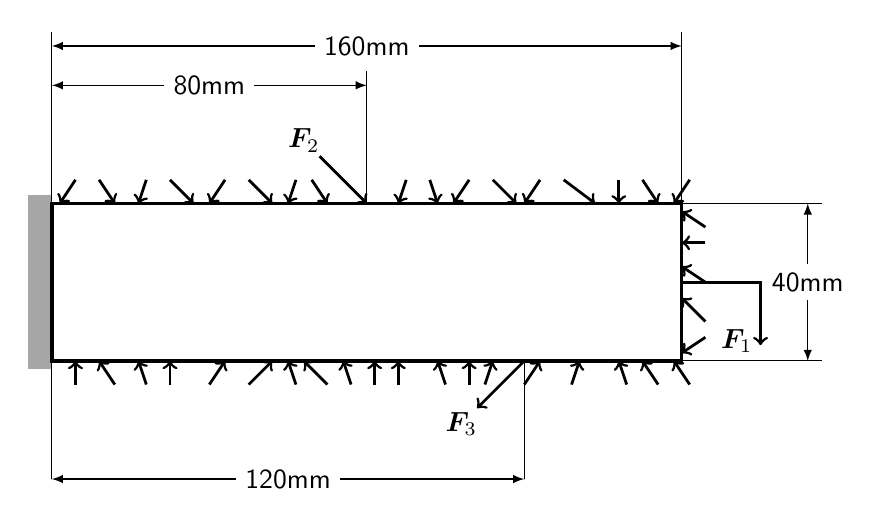
\begin{tikzpicture}
        \draw[fill,color=gray!70] (0,-0.1) rectangle (-0.3,2.1);
        \node [align=center, body,line width=1.2pt,minimum height=2cm,minimum width=8cm,anchor=south west] (body1) at (0,0) {};
        \draw (body1.south east) -- ++(1.6,0) coordinate (D1) -- +(5pt,0);
        \draw (body1.north east) -- ++(1.6,0) coordinate (D2) -- +(5pt,0);
        \draw [dimen] (D1) -- (D2) node {40mm};

        \draw (body1.north west) -- ++(0,2) coordinate (D1) -- +(0,5pt);
        \draw (body1.north east) -- ++(0,2) coordinate (D2) -- +(0,5pt);
        \draw [dimen] (D1) -- (D2) node {160mm};

        \draw[->,line width=1pt] (8,1) -- (9,1) -- (9,0.2);
        \node (arrowhead) at (8.7,0.25) {$\bm{F}_1$};

        \draw (body1.north west) -- ++(0,1.5) coordinate (D1) -- +(0,5pt);
        \draw (4,2) -- ++(0,1.5) coordinate (D2) -- +(0,5pt);
        \draw [dimen] (D1) -- (D2) node {80mm};

        \draw[->,line width=1pt] (3.4,2.6) -- (4,2);
        \node (arrowhead) at (3.2,2.8) {$\bm{F}_2$};

        \draw (body1.south west) -- ++(0,-1.5) coordinate (D1) -- +(0,5pt);
        \draw (6,0) -- ++(0,-1.5) coordinate (D2) -- +(0,5pt);
        \draw [dimen] (D1) -- (D2) node {120mm};

        \draw[->,line width=1pt] (6,0) -- (5.4,-0.6);
        \node (arrowhead) at (5.2,-0.8) {$\bm{F}_3$};

        \draw[->,line width=1pt] (0.3,2.3) -- (0.1,2);
        \draw[->,line width=1pt] (0.6,2.3) -- (0.8,2);
        \draw[->,line width=1pt] (1.2,2.3) -- (1.1,2);
        \draw[->,line width=1pt] (1.5,2.3) -- (1.8,2);
        \draw[->,line width=1pt] (2.2,2.3) -- (2.0,2);
        \draw[->,line width=1pt] (2.5,2.3) -- (2.8,2);
        \draw[->,line width=1pt] (3.1,2.3) -- (3.0,2);
        \draw[->,line width=1pt] (3.3,2.3) -- (3.5,2);
        \draw[->,line width=1pt] (4.5,2.3) -- (4.4,2);
        \draw[->,line width=1pt] (4.8,2.3) -- (4.9,2);
        \draw[->,line width=1pt] (5.3,2.3) -- (5.1,2);
        \draw[->,line width=1pt] (5.6,2.3) -- (5.9,2);
        \draw[->,line width=1pt] (6.2,2.3) -- (6.0,2);
        \draw[->,line width=1pt] (6.5,2.3) -- (6.9,2);
        \draw[->,line width=1pt] (7.2,2.3) -- (7.2,2);
        \draw[->,line width=1pt] (7.5,2.3) -- (7.7,2);
        \draw[->,line width=1pt] (8.1,2.3) -- (7.9,2);

        \draw[->,line width=1pt] (0.3,-0.3) -- (0.3,0);
        \draw[->,line width=1pt] (0.8,-0.3) -- (0.6,0);
        \draw[->,line width=1pt] (1.2,-0.3) -- (1.1,0);
        \draw[->,line width=1pt] (1.5,-0.3) -- (1.5,0);
        \draw[->,line width=1pt] (2.0,-0.3) -- (2.2,0);
        \draw[->,line width=1pt] (2.5,-0.3) -- (2.8,0);
        \draw[->,line width=1pt] (3.1,-0.3) -- (3.0,0);
        \draw[->,line width=1pt] (3.5,-0.3) -- (3.2,0);
        \draw[->,line width=1pt] (3.8,-0.3) -- (3.7,0);
        \draw[->,line width=1pt] (4.1,-0.3) -- (4.1,0);
        \draw[->,line width=1pt] (4.4,-0.3) -- (4.4,0);
        \draw[->,line width=1pt] (5.0,-0.3) -- (4.9,0);
        \draw[->,line width=1pt] (5.3,-0.3) -- (5.3,0);
        \draw[->,line width=1pt] (5.5,-0.3) -- (5.6,0);
        \draw[->,line width=1pt] (6.0,-0.3) -- (6.2,0);
        \draw[->,line width=1pt] (6.6,-0.3) -- (6.7,0);
        \draw[->,line width=1pt] (7.3,-0.3) -- (7.2,0);
        \draw[->,line width=1pt] (7.7,-0.3) -- (7.5,0);
        \draw[->,line width=1pt] (8.1,-0.3) -- (7.9,0);

        \draw[->,line width=1pt] (8.3,0.3) -- (8.0,0.1);
        \draw[->,line width=1pt] (8.3,0.5) -- (8.0,0.8);
        \draw[->,line width=1pt] (8.3,1.0) -- (8.0,1.2);
        \draw[->,line width=1pt] (8.3,1.5) -- (8.0,1.5);
        \draw[->,line width=1pt] (8.3,1.7) -- (8.0,1.9);
    \end{tikzpicture} \newline
  }
  \caption{Cantilever beam problem. $\bm{F}_2$ and $\bm{F}_3$ are at 45 degree angles.}
  \label{fig:CantBeam}
\end{figure}


      The 2D cantilever beam problem shown in Figure \ref{fig:CantBeam} was used to run the experiments. A ground mesh of plane stress quadrilateral elements was used, where each element is a square of side length $1 \text{ mm}$, and a sheet thickness of $1 \text{ mm}$. Linear iso-parametric interpolation functions were used for the field and geometric basis functions. A Young's modulus of 1 MPa and Poisson's ratio of 0.3 were used. Finally, a chequerboard density filter for unstructured meshes was used with a radius of 2 mm \citep{Huang2010a}. A 3D version of the problem above was also solved. Details of the 3D problem and the results are shown in appendix section \ref{app1}.

      Three variants of the cantilever beam problem were solved:
      \begin{enumerate}
        \item Minimization of the mean compliance $\mu_C$ subject to a volume constraint with a volume fraction of 0.4,
        \item Minimization of a weighted sum of the mean and standard deviation (mean-std) of the compliance $\mu_C + 2.0 \sigma_C$ subject to a volume constraint with a volume fraction of 0.4, and
        \item Volume minimization subject to a maximum compliance constraint with a compliance threshold of $70000 \text{ Nmm}$.
      \end{enumerate}
      A total of 1000 load scenarios were sampled from:
      \begin{align}
        \bm{f}_i = s_1 \bm{F}_1 + s_2 \bm{F}_2 + s_3 \bm{F}_3 + \frac{1}{7} \sum_{j=4}^{10} s_j \bm{F}_j
      \end{align}
      where $\bm{F}_1$, $\bm{F}_2$ and $\bm{F}_3$ are unit vectors with directions as shown in Figure \ref{fig:CantBeam}. $\bm{F}_2$ and $\bm{F}_3$ are at 45 degrees. $s_1$, $s_2$ and $s_3$ are identically and independently uniformly distributed random variables between -2 and 2. $\bm{F}_j$ for $j$ in $4 \dots 10$ are vectors with non-zeros at all the surface degrees of freedom without a Dirichlet boundary condition. The non-zero values are identically and independently normally distributed random variables with mean 0 and standard deviation 1. $s_j$ for $j$ in $4 \dots 10$ are also identically and independently normally distributed random variables with mean 0 and standard deviation 1. The same loading scenarios were used for the 3 test problems. Let $\bm{F}$ be the matrix whose columns are the sampled $\bm{f}_i$ vectors. The way the loading scenarios are defined, the rank of $\bm{F}$ can be at most 10 and was actually exactly 10 in our experiments. Given the low rank structure of $\bm{F}$, the SVD approaches should be expected to be significantly more efficient than their naive counterparts.

    \subsubsection{3D cantilever beam}

      A 3D version of the 2D cantilever beam test problem above was also solved using the methods proposed. A 60 mm x 20 mm x 20 mm 3D cantilever beam was used with hexahedral elements of cubic shape and side length of 1 mm. The loads $\bm{F}_1$, $\bm{F}_2$ and $\bm{F}_3$ were positioned at (60, 10, 10), (30, 20, 10) and (40, 0, 10) where the coordinates represent the length, height and depth respectively. The remaining loads and multipliers were sampled from the same distributions as the 2D problem. A density filter radius of 3 mm was also used for the 3D problem.

  \subsection{Settings}

    The value of $x_{min}$ used was $0.001$ for all problems and algorithms. Penalization was done prior to interpolation to calculate $\bm{\rho}$ from $\bm{x}$. A power penalty function and a regularized Heaviside projection were used. All of the problems were solved using 2 continuation SIMP routines. The first incremented the penalty value from $p = 1$ to $p = 6$ in increments of 0.5. Then the Heaviside projection parameter $\beta$ was incremented from $\beta = 0$ to $\beta = 20$ in increments of 4 keeping the penalty value fixed at 6. An exponentially decreasing tolerance from $1e-3$ to $1e-4$ was used for both continuations.

    The mean and mean-std compliance minimization SIMP subproblems problems were solved using the method of moving asymptotes (MMA) algorithm \cite{Svanberg1987}. MMA parameters of $s_{init} = 0.5$, $s_{incr} = 1.1$ and $s_{decr} = 0.7$ were used as defined in the MMA paper with a maximum of 1000 iterations for each subproblem. The dual problem of the convex approximation was solved using a log-barrier box-constrained nonlinear optimization solver, where the barrier problem was solved using the nonlinear CG algorithm for unconstrained nonlinear optimization \citep{Nocedal2006} as implemented in Optim.jl \footnote{https://github.com/JuliaNLSolvers/Optim.jl} \citep{KMogensen2018}. The nonlinear CG itself used the line search algorithm from \cite{Hager2006} as implemented in LineSearches.jl \footnote{https://github.com/JuliaNLSolvers/LineSearches.jl}. The stopping criteria used was the one adopted by the KKT solver, IPOPT \citep{Wachter2006}. This stopping criteria is less scale sensitive than the KKT residual as it scales down the residual by a value proportional to the mean absolute value of the Lagrangian multipliers.

    The maximum compliance constrained SIMP subproblems were solved using a primal-dual augmented Lagrangian method \citep{Bertsekas1996}. The inequality constraints were relaxed resulting in a box constrained max-min primal-dual problem. A projected gradient descent algorithm was used for the primal and dual problems with a backtracking line search. The maximum step size of the line search was initialized to 1 and adapted to be 1.5 the step size of the previous line search for both the primal and dual problems. A total of 10 dual iterations were used with a maximum of 50 primal iterations per dual iteration. The IPOPT termination criteria above was also used here. To regularize the scale of the problem, the compliance constraints were divided by the maximum compliance at the full ground mesh design. A trust region of 0.1 was used. An initial quadratic penalty coefficient of 0.1 was used with a growth factor of 3 in every dual iteration. Finally, an initial solution of 1.0 for all the primal variables and 1 for all the Lagrangian multipliers was used.

\section{Results and Discussion} \label{sec:results}

  \subsection{Speed comparison}

    Tables \ref{tab:time_mean} and \ref{tab:time_std} show the values computed for the mean compliance $\mu_C$ and its standard deviation $\sigma_C$ respectively together with the time required to compute their values and gradients using: the exact naive approach (Exact-Naive) and the exact method with SVD (Exact-SVD). As expected, the proposed exact SVD approach computes the exact mean compliance or its standard deviation and their gradient in a small fraction of the time it takes to compute them using the naive approaches.

    \begin{table}[h!]
     \centering
     \caption{The table shows the function values of $\mu_C$ computed using the naive exact method (Exact-Naive) and the exact method with SVD (Exact-SVD). The table also shows the time required to compute $\mu_C$ and its gradient in each case.}
     \begin{tabular}{|c|c|c|}
      \hline
      Method & $\mu_C$ (Nmm) & Time (s) \\
      \hline
      \hline
      Exact-Naive & 3328.7 & 24.2 \\
      \hline
      Exact-SVD & 3328.7 & 0.4 \\
      \hline
     \end{tabular}
     \label{tab:time_mean}
    \end{table}

    \begin{table}[h!]
     \centering
     \caption{The table shows the function values of $\sigma_C$ and its gradients for a full ground mesh computed using the naive exact method (Exact-Naive) and the exact method with SVD (Exact-SVD). The table also shows the time required to compute $\sigma_C$ and its gradient in each case.}
     \begin{tabular}{|c|c|c|}
      \hline
      Method & $\sigma_C$ (Nmm) & Time (s) \\
      \hline
      \hline
      Exact-Naive & 4172.8 & 28.0 \\
      \hline
      Exact-SVD & 4172.8 & 1.5 \\
      \hline
     \end{tabular}
     \label{tab:time_std}
    \end{table}

  \subsection{Optimization}

    In this section, a number of stochastic, risk-averse and robust compliance-based optimization problems are solved using the proposed methods. Figure \ref{fig:flowchart} shows the experiments' workflow.

    \begin{figure}
      \centering
      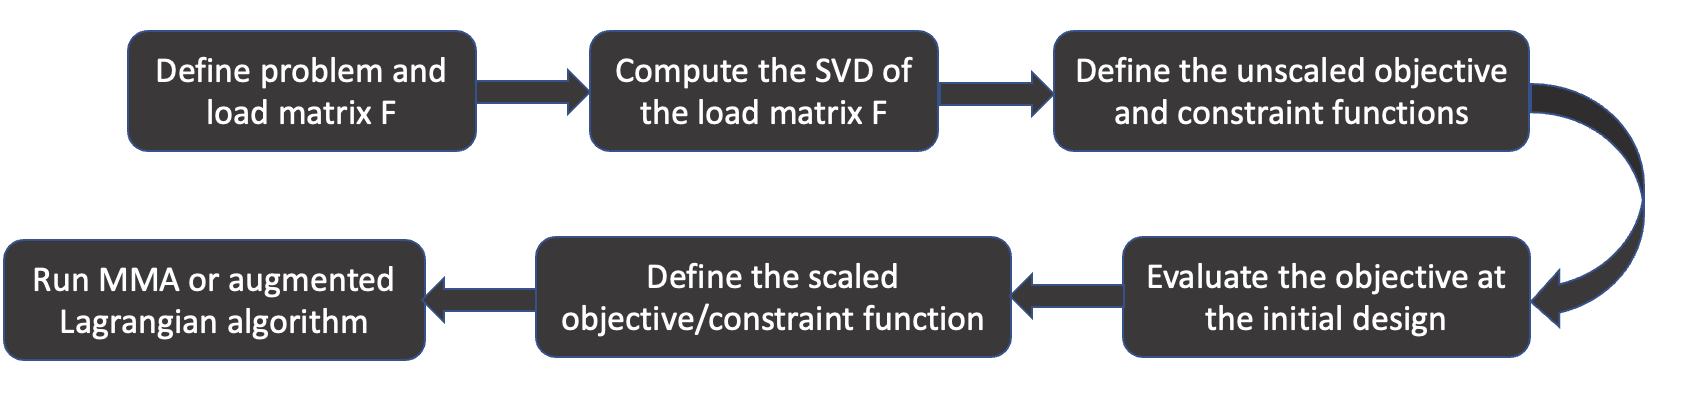
\includegraphics[width=\textwidth]{./images/robust_exact/flowchart.png}
      \caption{Flowchart of the experiments' workflow. Only the mean compliance objective, mean-std compliance objective or maximum compliance constraint are scaled by the inverse of their initial value. The volume function is not scaled.}
      \label{fig:flowchart}
    \end{figure}

    \subsubsection{Mean compliance minimization}

      To demonstrate the effectiveness of the proposed approaches, the 2D and 3D cantilever beam problems described in section \ref{sec:exp_impl} were solved using the proposed SVD-based methods. Table \ref{tab:mean_stats} shows the statistics of the final optimal solutions obtained by minimizing the mean compliance subject to the volume fraction constraint using the SVD-based method to evaluate the mean compliance. The optimal topologies are shown in Figures \ref{fig:mean} and \ref{fig:exact_mean_3d}.

      \begin{figure}
        \centering
        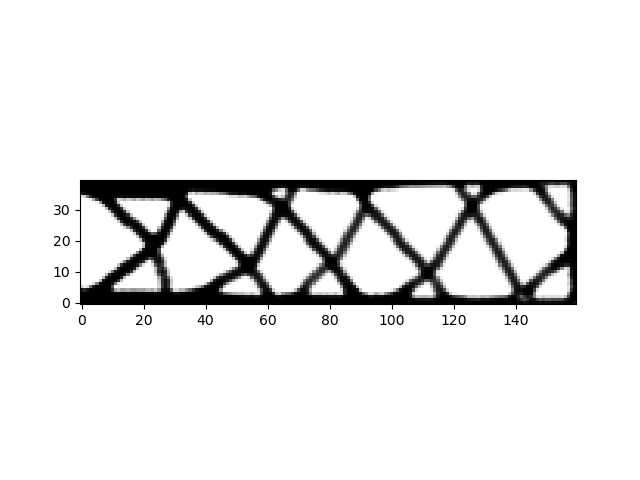
\includegraphics[width=\textwidth]{./images/robust_exact/exact_svd_mean_csimp.png}
        \caption{Optimal topology of the mean compliance minimization problem using continuation SIMP and the SVD-based method for evaluating the mean compliance.}
        \label{fig:mean}
      \end{figure}

      \begin{figure}
        \begin{subfigure}[t]{0.45\textwidth}
          \centering
          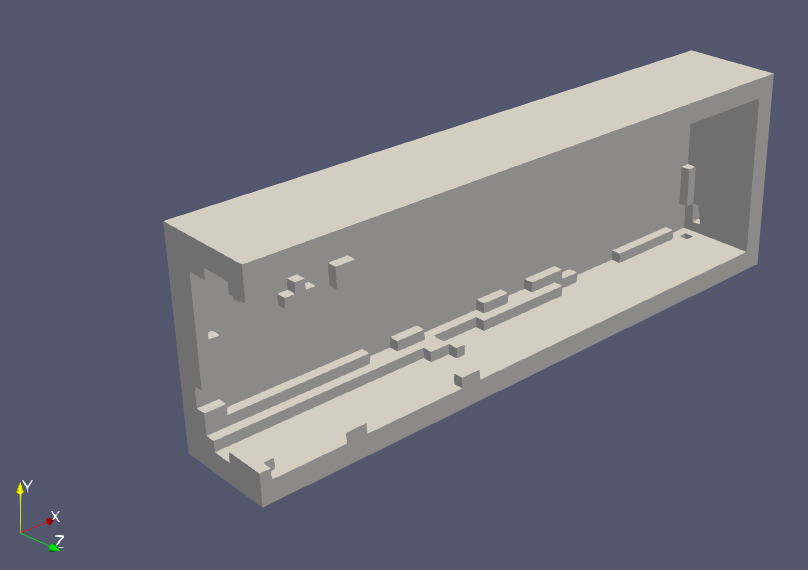
\includegraphics[width=1\textwidth]{./images/robust_exact/exact_mean_1.png}
          \caption{Left half}
        \end{subfigure}
        \begin{subfigure}[t]{0.45\textwidth}
          \centering
          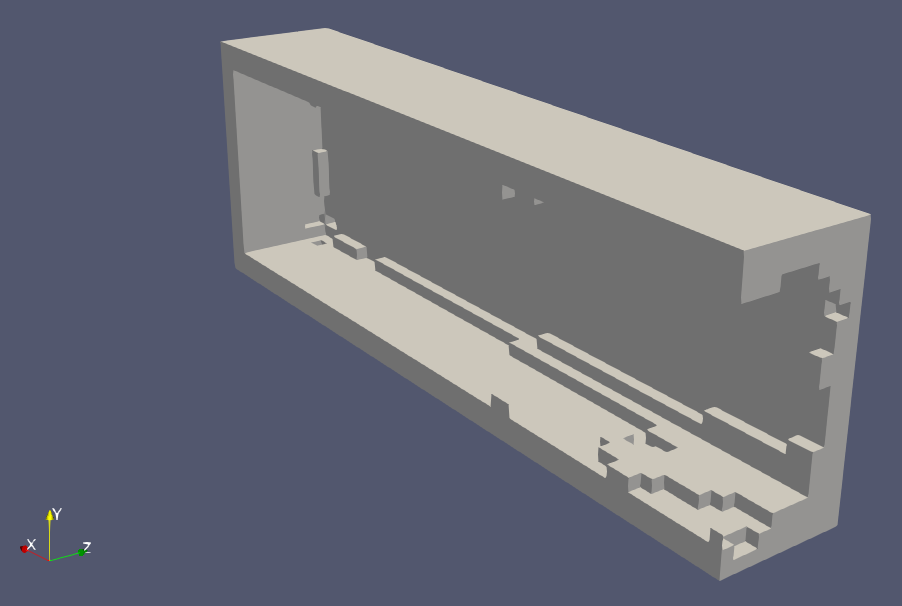
\includegraphics[width=1\textwidth]{./images/robust_exact/exact_mean_2.png}
          \caption{Right half}
        \end{subfigure}
        \caption{Cut views of the optimal topologies of the 3D mean compliance minimization problem using exact method with SVD.}
        \label{fig:exact_mean_3d}
      \end{figure}

      \begin{table}[h!]
       \centering
       \caption{Summary statistics of the load compliances of the optimal solutions of the 2D and 3D mean compliance minimization problems using the SVD-based method to evaluate the mean compliance.}
       \begin{tabular}{|c|c|c|}
        %1.1 - 0.7 - 0.5
        \hline
        Compliance Stat & 2D & 3D \\
        \hline
        \hline
        $\mu_C$ (Nmm) & 9392.8 & 22072.1 \\
        \hline
        $\sigma_C$ (Nmm) & 9688.8 & 16628.7 \\
        \hline
        $C_{max}$ (Nmm) & 125455.0 & 184055.0 \\
        \hline
        $C_{min}$ (Nmm) & 467.9 & 1785.8 \\
        \hline
        $V$ & 0.400 & 0.400 \\
        \hline
        $Time$ (s) & 491.5 & 3849.6 \\
        \hline
       \end{tabular}
       \label{tab:mean_stats}
      \end{table}

    \subsubsection{Mean-std compliance minimization}

      Similarly, Table \ref{tab:mean_std_stats} shows the statistics of the final solutions of the 2D and 3D mean-std minimization problems solved using the SVD-based method. The optimal topologies are shown in Figures \ref{fig:mean_std} and \ref{fig:exact_mean_std_3d}. The algorithm converged to reasonable, feasible designs. Additionally, as expected the mean-std minimization algorithm converged to solutions with lower compliance standard deviations but higher mean compliances compared to the mean minimization algorithm.

      \begin{figure}
        \centering
        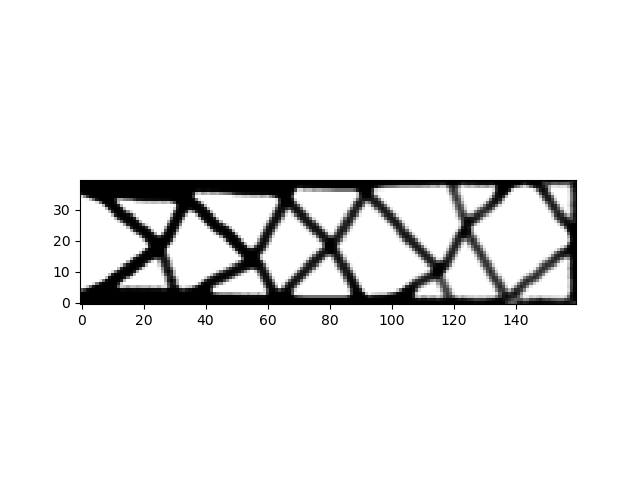
\includegraphics[width=\textwidth]{./images/robust_exact/exact_svd_mean_std_csimp.png}
        \caption{Optimal topology of the mean-std compliance minimization problem using continuation SIMP and the SVD-based method to compute the mean-std.}
        \label{fig:mean_std}
      \end{figure}

      \begin{figure}
        \begin{subfigure}[t]{0.45\textwidth}
          \centering
          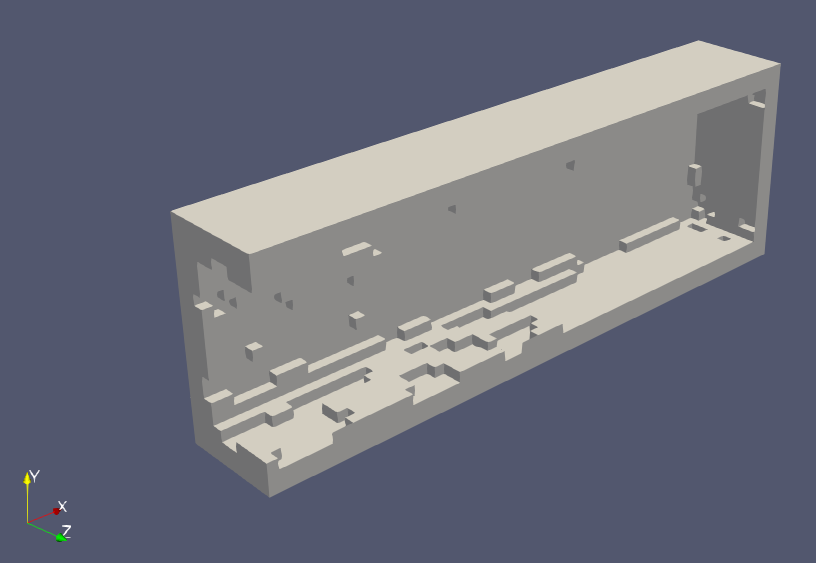
\includegraphics[width=1\textwidth]{./images/robust_exact/exact_mean_std_1.png}
          \caption{Left half}
        \end{subfigure}
        \begin{subfigure}[t]{0.45\textwidth}
          \centering
          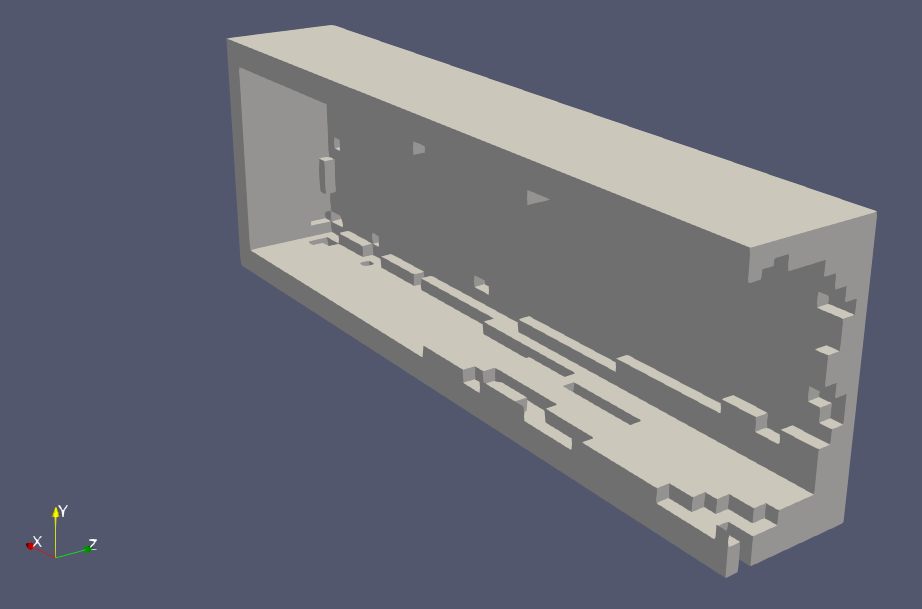
\includegraphics[width=1\textwidth]{./images/robust_exact/exact_mean_std_2.png}
          \caption{Right half}
        \end{subfigure}
        \caption{Cut views of the optimal topologies of the 3D mean-std compliance minimization problem using the exact method with SVD.}
        \label{fig:exact_mean_std_3d}
      \end{figure}

      \begin{table}[h!]
       \centering
       \caption{Summary statistics of the load compliances of the optimal solutions of the 2D and 3D mean-std compliance minimization problems using the SVD-based method to evaluate the mean-std compliance.}
       \begin{tabular}{|c|c|c|}
        \hline
        Compliance Stat & 2D & 3D \\
        \hline
        \hline
        $\mu_C (Nmm) $ & 9796.9 & 22216.7 \\
        \hline
        $\sigma_C (Nmm) $ & 9240.0 & 16220.2 \\
        \hline
        $\mu_C + 2.0 \sigma_C (Nmm) $ & 28283.7 & 54848.8 \\
        \hline
        $C_{max}$ (Nmm) & 117883.1 & 176153.2 \\
        \hline
        $C_{min}$ (Nmm) & 527.7 & 1872.0 \\
        \hline
        $V$ & 0.400 & 0.400 \\
        \hline
        Time (s) & 229.8 & 3528.2 \\
        \hline
       \end{tabular}
       \label{tab:mean_std_stats}
      \end{table}

      To highlight the effect of the multiple $m$ of the standard deviation in the objective $\mu_C + m \times \sigma_C$, the same problem was solved for different values of $m$. Figure \ref{fig:mean_std_profile} shows the profile of the mean and standard deviation of the compliance. Interestingly due to the non-convexity of the problem, increasing the standard deviation's multiple can sometimes lead to a simultaneous increase or reduction in the mean and standard deviation of the compliance. The different optimal topologies are shown in Figure \ref{fig:mean_m_std_2d}.

      \begin{figure}
        \centering
        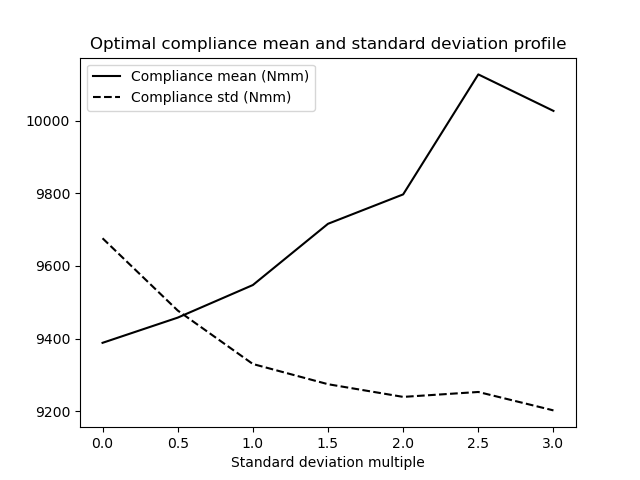
\includegraphics[width=\textwidth]{./images/robust_exact/mean_std_profile.png}
        \caption{Profile of the optimal mean and standard deviation of the compliance for different standard deviation multiples in the objective.}
        \label{fig:mean_std_profile}
      \end{figure}

      \begin{figure*}
        \begin{subfigure}[t]{0.45\textwidth}
          \centering
          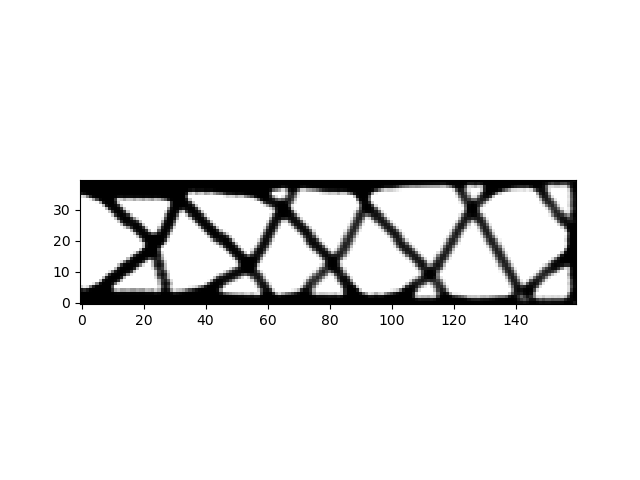
\includegraphics[width=1\textwidth]{./images/robust_exact/exact_svd_mean_0std_csimp.png}
          \caption{$m = 0$}
        \end{subfigure}
        \begin{subfigure}[t]{0.45\textwidth}
          \centering
          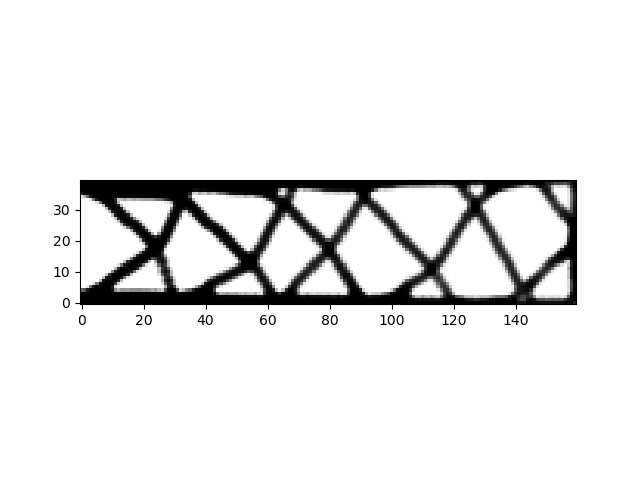
\includegraphics[width=1\textwidth]{./images/robust_exact/exact_svd_mean_5std_csimp.png}
          \caption{$m = 0.5$}
        \end{subfigure}
        \begin{subfigure}[t]{0.45\textwidth}
          \centering
          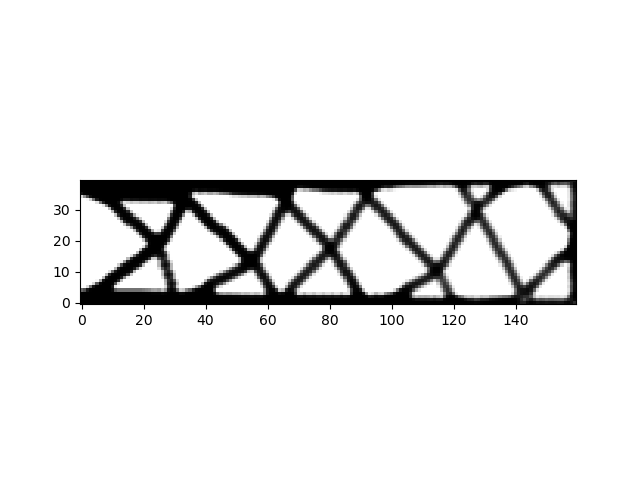
\includegraphics[width=1\textwidth]{./images/robust_exact/exact_svd_mean_10std_csimp.png}
          \caption{$m = 1.0$}
        \end{subfigure}
        \begin{subfigure}[t]{0.45\textwidth}
          \centering
          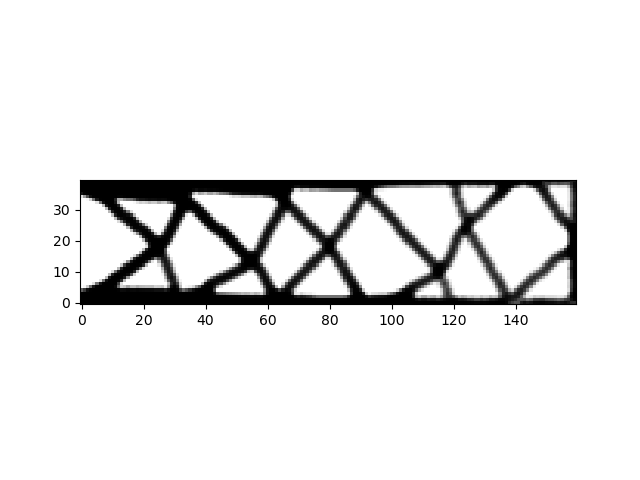
\includegraphics[width=1\textwidth]{./images/robust_exact/exact_svd_mean_15std_csimp.png}
          \caption{$m = 1.5$}
        \end{subfigure}
        \begin{subfigure}[t]{0.45\textwidth}
          \centering
          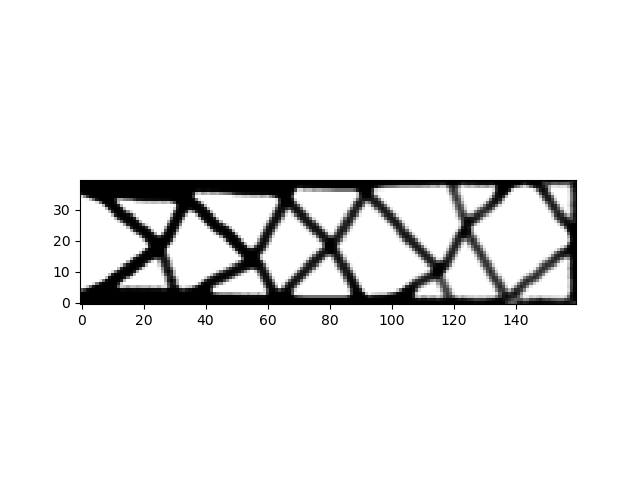
\includegraphics[width=1\textwidth]{./images/robust_exact/exact_svd_mean_20std_csimp.png}
          \caption{$m = 2.0$}
        \end{subfigure}
        \begin{subfigure}[t]{0.45\textwidth}
          \centering
          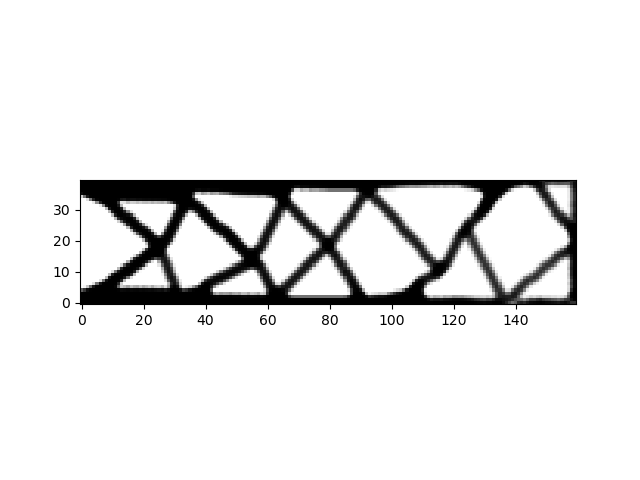
\includegraphics[width=1\textwidth]{./images/robust_exact/exact_svd_mean_25std_csimp.png}
          \caption{$m = 2.5$}
        \end{subfigure}
        \begin{subfigure}[t]{0.45\textwidth}
          \centering
          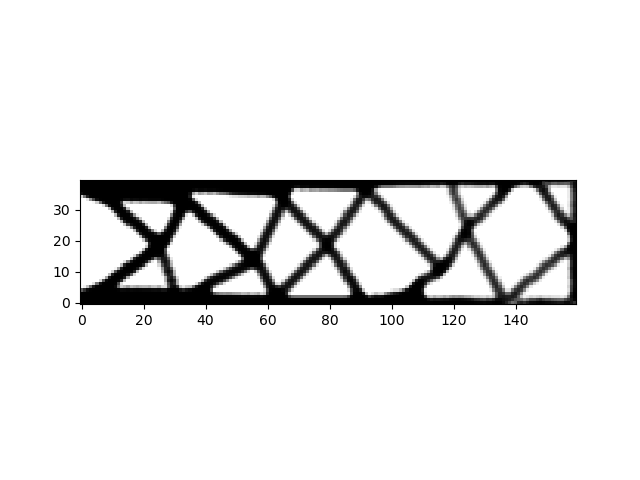
\includegraphics[width=1\textwidth]{./images/robust_exact/exact_svd_mean_30std_csimp.png}
          \caption{$m = 3.0$}
        \end{subfigure}
        \caption{Optimal topologies of the 2D mean-std compliance minimization problem using different standard deviation multiples $m$ in the objective $\mu_C + m \sigma_C$.}
        \label{fig:mean_m_std_2d}
      \end{figure*}

    \subsubsection{Maximum compliance constrained optimization}

      The 2D and 3D maximum compliance constrained volume minimization problems were solved using the SVD-based approach. The 2D optimal topology, shown in Figure \ref{fig:max}, had a volume fraction of 0.584 and a maximum compliance of 69847.0 Nmm and was reached in 662.7 s. The 3D optimal topology, shown in Figure \ref{fig:max_3d}, had a volume fraction of 0.791 and a maximum compliance of 68992.4 Nmm and was reached in 43740.6 s.

      \begin{figure}
        \centering
        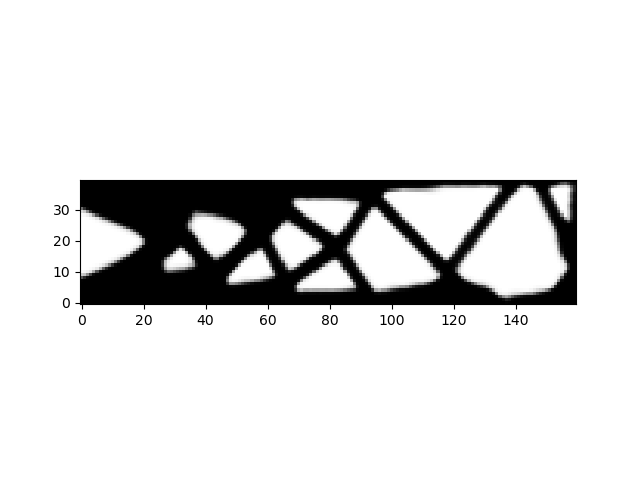
\includegraphics[width=\textwidth]{./images/robust_exact/exact_svd_max_csimp.png}
        \caption{Optimal topology of the volume minimization problem subject to a maximum compliance constraint using continuation SIMP and the augmented Lagrangian method with the exact SVD approach. The maximum compliance of the design above is 69847.0 Nmm and the volume fraction is 0.584.}
        \label{fig:max}
      \end{figure}

      \begin{figure}
        \centering
        \begin{subfigure}[t]{0.45\textwidth}
          \centering
          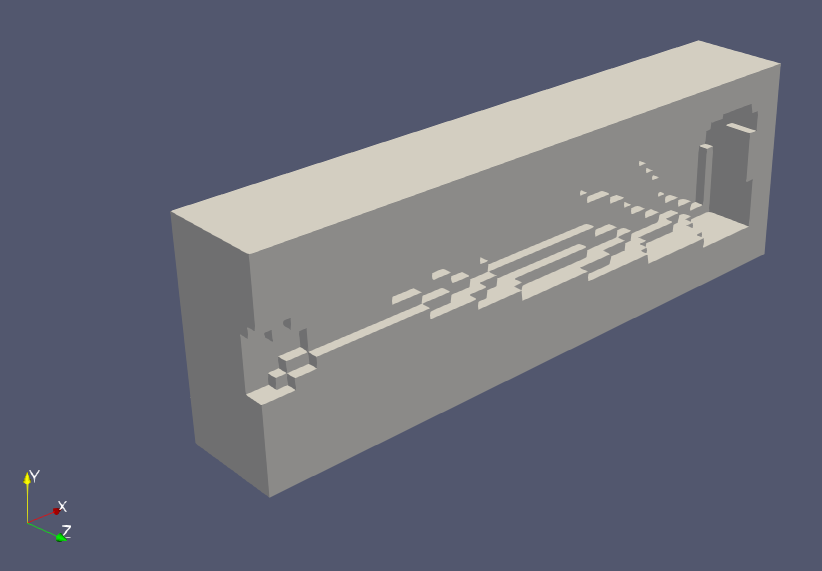
\includegraphics[width=1\textwidth]{./images/robust_exact/exact_max_1.png}
          \caption{Left half}
        \end{subfigure}
        \begin{subfigure}[t]{0.45\textwidth}
          \centering
          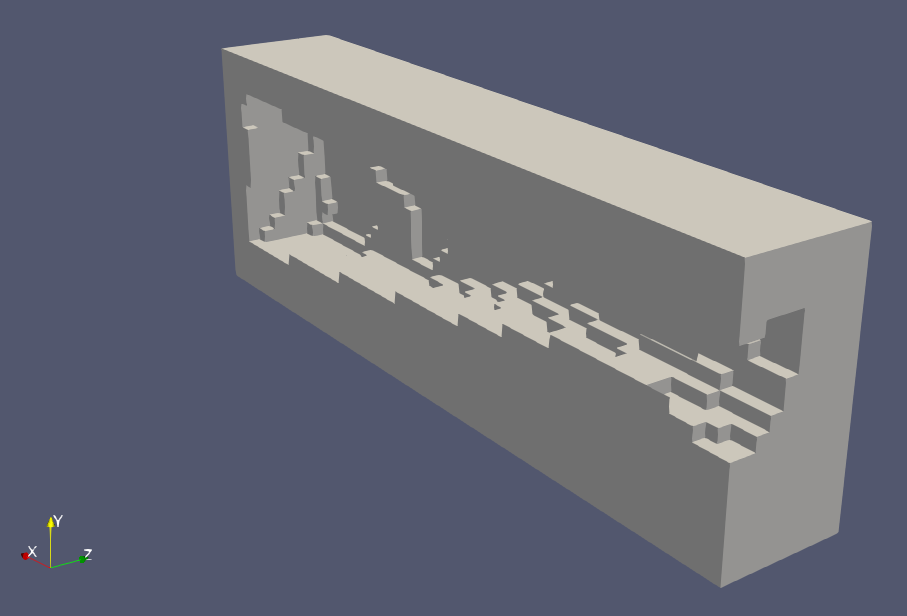
\includegraphics[width=1\textwidth]{./images/robust_exact/exact_max_2.png}
          \caption{Right half}
        \end{subfigure}
        \caption{Cut views of the 3D optimal topology of the volume minimization problem subject to a maximum compliance constraint using continuation SIMP and the augmented Lagrangian method with the exact SVD approach. The maximum compliance of the design above is 68992.4 Nmm and the volume fraction is 0.791.}
        \label{fig:max_3d}
      \end{figure}

\section{Conclusion} \label{sec:conclusion}

  In this chapter, a number of exact methods were proposed to handle load uncertainty in compliance topology optimization problems where the uncertainty is described in the form of a set of finitely many loading scenarios. By exploiting low rank structures in loading scenarios, significant performance improvements were achieved using novel SVD-based methods. Such improvement was demonstrated via complexity analysis and computational experiments. The methods presented here are fundamentally data-driven in the sense that no probability distributions or domains are assumed for the loading scenarios. This sets this work apart from most of the literature in the domain of stochastic and robust topology optimization where a distribution or domain is assumed. Additionally, the methods proposed here were shown to be particularly suitable with the augmented Lagrangian algorithm when dealing with maximum compliance constraints.

\newpage

	\let\cleardoublepage\clearpage
%	\null\newpage
	\chapter{Approximate compliance-based optimization with finitely many loading scenarios}\thispagestyle{EmptyHeader}
\label{chp:4}

\section{Introduction}

In the previous chapter, a few exact methods for handling a large number of loading scenarios in compliance-based problems were proposed based on the singular value decomposition (SVD), where the loading matrix $\bm{F}$ has a low rank and/or a few degrees of freedom are loaded. However when these conditions are not satisfied, the SVD based approach may not be efficient enough. In particular, there are 2 limitations to the SVD-based approaches:
\begin{enumerate}
  \item The computational time complexity of computing the SVD of $\bm{F}$ is \newline $O(min(L, n_{dofs})^2 max(L, n_{dofs}))$ if the loads are dense, where $L$ is the number of loading scenarios and $n_{dofs}$ is the number of degrees of freedom, which can be computationally prohibitive for large problems.
  \item The load matrix may not be low rank.
\end{enumerate}

In this chapter, a few SVD-free approximate methods will be proposed to estimate the value and gradient of:
\begin{enumerate}
    \item The mean compliance
    \item The standard deviation of the compliance
    \item A class of scalar-valued functions of load compliances satisfying a few conditions
\end{enumerate}

In this chapter, computationally efficient approximation schemes are proposed to approximate the values and gradients of the mean compliance, its standard deviation as well as a class of scalar valued function of individual load compliances subject to a finite number of possible loading scenarios. These approaches can be used in risk-averse compliance minimization.

\section{Proposed algorithms}

  \subsection{Approximating the compliance sample mean and its gradient} \label{sec:proposed_mean}

    The mean compliance can be formulated as a trace function: $\mu_C = \frac{1}{L} tr(\bm{F}^T \bm{K}^{-1} \bm{F})$. \cite{Zhang2017a} showed that Hutchinson's trace estimator \cite{Hutchinson1990} can be used to accurately estimate the compliance for a large number of load scenarios using a relatively small number of linear system solves. Hutchinson's trace estimator is given by:
      \begin{align}
        & tr(\bm{A}) = E(\bm{v}^T \bm{A} \bm{v}) \approx \frac{1}{N} \sum_{i=1}^{N} \bm{v}_i^T \bm{A} \bm{v}_i
      \end{align}
      where $\bm{v}$ is a random vector with each element independently distributed with 0 mean and unit variance, $\bm{v}_i$ are samples of the random vector $\bm{v}$, also known as probing vectors, and $N$ is the number of such probing vectors. One common distribution used for the elements of $\bm{v}$ is the Rademacher distribution which is a discrete distribution with support $\{-1, 1\}$ each of which has a probability of 0.5. Hutchinson proved that an estimator with the Rademacher distribution for $\bm{v}$ will have the least variance among all other distributions. Let $\bm{A} = \bm{F}^T \bm{K}^{-1} \bm{F}$. The number of linear system solves required to compute the mean compliance $\frac{1}{L} tr(\bm{A})$ using the naive approach is $L$. However, when using Hutchinson's estimator, that number becomes the number of probing vectors $N$. In general, a good accuracy can be obtained for $N \ll L$. Other than the linear system solves, the time complexity of the remaining work using the trace estimation method is $O(N \times n_{dofs} \times L)$ mostly spent on finding $\bm{F} \bm{v}_i$ for all $i$. If only a small number of degrees of freedom $n_{loaded}$ are loaded, the complexity of the remaining work reduces to $O(N \times n_{loaded} \times L)$.

      Let $\bm{z}_i = \bm{K}^{-1} \bm{F} \bm{v}_i$ be cached from the trace computation. The elements of the gradient of the trace estimate with respect to $\bm{\rho}$ are given by:
      \begin{align}
       \mu_C(\bm{\rho}) & = \frac{1}{L \times N} \sum_i^N \bm{z}_i^T \bm{K} \bm{z}_i \\
       \frac{\partial \mu_C}{\partial \rho_e} & = \frac{1}{L \times N} \sum_{i=1}^N -\bm{z}_i^T \bm{K}_e \bm{z}_i
      \end{align}
      The additional time complexity of computing the gradient of the trace estimate after computing the trace is therefore $O(N \times n_E)$. For a detailed derivation of the partial above, see the appendix.

      \begin{table}
       \centering
       \caption{Summary of the computational cost of the algorithms discussed to calculate the mean compliance and its gradient. \#Lin is the number of linear system solves required.}
       \begin{tabular}{| m{3cm} | m{0.7cm} | m{4cm} | m{5cm}|} 
        \hline
        \multirow{2}{3em}{Method} & \multirow{2}{2em}{\#Lin} & \multicolumn{2}{c|}{Time complexity of additional work} \\\cline{3-4}
        & & Dense & Sparse \\
        \hline
        \hline
        Exact & \(L\) & \(O(L \times (n_{dofs} + n_E))\) & \(O(L \times (n_{loaded} + n_E))\) \\
        \hline
        Trace estimation & \(N\) & \(O(N \times (n_{dofs} \times L + n_E))\) & \(O(N \times (L \times n_{loaded} + n_E))\) \\
        \hline
       \end{tabular}
       \label{tab:perf_mean}
      \end{table}

  \subsection{Approximating scalar-valued function of load compliances and its gradient} \label{sec:proposed_risk}

    The above scheme for approximating the sample mean compliance can be generalized to handle the sample variance and standard deviations. The sample variance of the compliance $C$ is given by $\sigma_C^2 = \frac{1}{L-1} \sum_{i=1}^L (C_i - \mu_C)^2$. The sample standard deviation $\sigma_C$ is the square root of the variance. Let $\bm{C}$ be the vector of compliances $C_i$, one for each load scenario. In vector form, $\sigma_C^2 = \frac{1}{L-1} (\bm{C} - \mu_C \bm{1})^T (\bm{C} - \mu_C \bm{1})$. $\bm{C} = diag(\bm{A})$ is the diagonal of the matrix $\bm{A} = \bm{F}^T \bm{K}^{-1} \bm{F}$.

    One can view the load compliances $\bm{C}$ as the diagonal of the matrix $\bm{F}^T \bm{K}^{-1} \bm{F}$. One way to estimate it is therefore to use a diagonal estimation method. One diagonal estimator directly related to Hutchinson's trace estimator was proposed by Bekas et al. \cite{Bekas2007}. The diagonal estimator can be written as follows:
      \begin{align}
       & diag(\bm{A}) = E(\bm{D}_{\bm{v}} \bm{A} \bm{v}) \approx \frac{1}{N} \sum_{i=1}^N \bm{D}_{\bm{v}_i} \bm{A} \bm{v}_i
      \end{align}
    where $diag(\bm{A})$ is the diagonal of $\bm{A}$ as a vector, $\bm{D}_{\bm{v}}$ is the diagonal matrix with a diagonal $\bm{v}$, $\bm{v}$ is a random vector distributed much like in Hutchinson's estimator, $\bm{v}_i$ are the probing vector instances of $\bm{v}$ and $N$ is the number of probing vectors. The sum of the elements of the diagonal estimator above gives us Hutchinson's trace estimator. Let $\bm{A} = \bm{F}^T \bm{K}^{-1} \bm{F}$:
      \begin{align}
       & \bm{C} = diag(\bm{\bm{F}^T \bm{K}^{-1} \bm{F}}) \approx \frac{1}{N} \sum_{i=1}^N \bm{D}_{\bm{v}_i} \bm{\bm{F}^T \bm{K}^{-1} \bm{F}} \bm{v}_i
      \end{align}
    Bekas et al. showed that using the deterministic basis of a Hadamard matrix as probing vectors $\bm{v}_i$ rather than random vectors increases the accuracy of the diagonal estimator. In this chapter, we do the same and use columns of a Hadamard matrix as probing vectors for the diagonal estimator. Given the diagonal estimate assuming $N \ll L$, one can estimate $\bm{C}$ using $N$ linear system solves, which can then be used to compute the sample variance and standard deviation. Other than the linear system solves, the additional work required above has a time complexity of $O(N \times n_{dofs} \times L)$. But if only a few $n_{loaded}$ degrees of freedom are loaded, the time complexity of the remaining work goes down to $O(N \times n_{loaded} \times L)$.

    The Jacobian of the compliances vector $\bm{C}$ with respect to $\bm{\rho}$, $\nabla_{\bm{\rho}} \bm{C}$ is simply the stacking of the transposes of the gradients of $C_i$, $\nabla_{\bm{\rho}} C_i$, for all $i$ to form a matrix with $L$ rows and $n_E$ columns. The Jacobian of the estimate of $\bm{C}$ is given by:
      \begin{align}
       & \nabla_{\bm{\rho}} \bm{C} \approx \frac{1}{N} \sum_{i=1}^N \bm{D}_{\bm{v}_i} \bm{\bm{F}}^T \bm{K}^{-1} \bm{F} \bm{v}_i = \frac{1}{N} \sum_{i=1}^N \bm{D}_{\bm{v}_i} \bm{F}^T \nabla_{\bm{\rho}} \bm{t}_i
      \end{align}
    where $\bm{t}_i = \bm{K}^{-1} \bm{F} \bm{v}_i$. The derivative $\frac{\partial \bm{t}_i}{\partial \rho_e} = -\bm{K}^{-1} \bm{K}_e \bm{t}_i$. Therefore:
      \begin{align}
       & \frac{\partial \bm{C}}{\partial \rho_e} \approx \frac{1}{N} \sum_{i=1}^N \bm{D}_{\bm{v}_i} \bm{\bm{F}}^T \bm{K}^{-1} \bm{K}_e \bm{K}^{-1} \bm{\bm{F}} \bm{v}_i
      \end{align}
    Note that to find the Jacobian in this case, one requires $L$ linear system solves to find $\bm{K}^{-1} \bm{F}$. However, with this many linear system solves one can use the exact method so there is no merit to using the diagonal estimation approach. This means that if the full Jacobian is required, the diagonal estimation method here is the wrong choice.

    However if only interested in $\nabla_{\bm{\rho}} \bm{C}(\bm{\rho})^T \bm{w}$, a more efficient approach can be used:
      \begin{align}
       \nabla_{\bm{\rho}} \bm{C}(\bm{\rho})^T \bm{w} & = \nabla_{\bm{\rho}} (\bm{C}(\bm{\rho})^T \bm{w}) = \nabla_{\bm{\rho}} tr(\bm{D}_{\bm{w}} \bm{F}^T \bm{K}^{-1} \bm{F})
      \end{align}
    Let $\bm{r}_i = \bm{K}^{-1} \bm{F} \bm{v}_i$ which are cached from the function value calculation, and let $\bm{t}_i = \bm{K}^{-1} \bm{F} \bm{D}_{\bm{w}} \bm{v}_i$.
      \begin{align}
       \frac{\partial \bm{C}(\bm{\rho})^T \bm{w}}{\partial \rho_e} & = -tr(\bm{D}_{\bm{w}} \bm{F}^T \bm{K}^{-1} \bm{K}_e \bm{K}^{-1} \bm{F}) \\
       & \approx -\frac{1}{N} \sum_{i=1}^N \bm{v}_i^T \bm{D}_{\bm{w}} \bm{F}^T \bm{K}^{-1} \bm{K}_e \bm{K}^{-1} \bm{F} \bm{v}_i \\
       & = -\frac{1}{N} \sum_{i=1}^N \bm{t}_i^T \bm{K}_e \bm{r}_i 
      \end{align}
    This means that at a cost of an additional $N$ linear system solves, one can compute the vectors $\bm{t}_i$ and then find the gradient of $\bm{C}^T \bm{w}$. Other than the linear system solves, the remaining work has a time complexity of $O(N \times (n_{dofs} \times L + n_E))$, $O(N \times n_{dofs} \times L)$ from the accumulation of $\bm{F} \bm{D}_{\bm{w}} \bm{v}_i$ and $O(N \times n_E)$ to evaluate the gradient given $\bm{t}_i$ and $\bm{r}_i$ for all $i$. If only a few degrees of freedom $n_{loaded}$ are loaded, then the complexity goes down to $O(N \times (n_{loaded} \times L + n_E))$.

    \begin{table}
        \centering
        \caption{Summary of the computational cost of the algorithms discussed to calculate the load compliances $\bm{C}$ as well as $\nabla_{\bm{\rho}} \bm{C}^T \bm{w}$ for any vector $\bm{w}$. \#Lin is the number of linear system solves required. This can be used to compute the variance, standard deviation as well as other scalar-valued functions of $\bm{C}$.}
        \begin{tabular}{|m{4cm} | m{0.7cm} | m{4cm} | m{5cm} |} 
         \hline
         \multirow{2}{3em}{Method} & \multirow{2}{2em}{\#Lin} & \multicolumn{2}{c|}{Time complexity of additional work} \\\cline{3-4}
         & & Dense & Sparse \\
         \hline
         \hline
         Exact & \(L\) & \(O(L \times (n_{dofs} + n_E))\) & \(O(L \times (n_{loaded} + n_E))\) \\
         \hline
         Diagonal estimation & \(2N\) & \(O(N \times (n_{dofs} \times L + n_E))\) & \(O(N \times (n_{loaded} \times L + n_E))\) \\
        \hline
       \end{tabular}
       \label{tab:perf_scalar}
    \end{table}

\section{Setup and Implementation} \label{sec:exp_impl}

  In this section, the most important implementation details and algorithm settings used in the experiments are presented.

  \subsection{Test problems}

    \begin{figure}
  \centering
  \resizebox{\textwidth}{!}{
    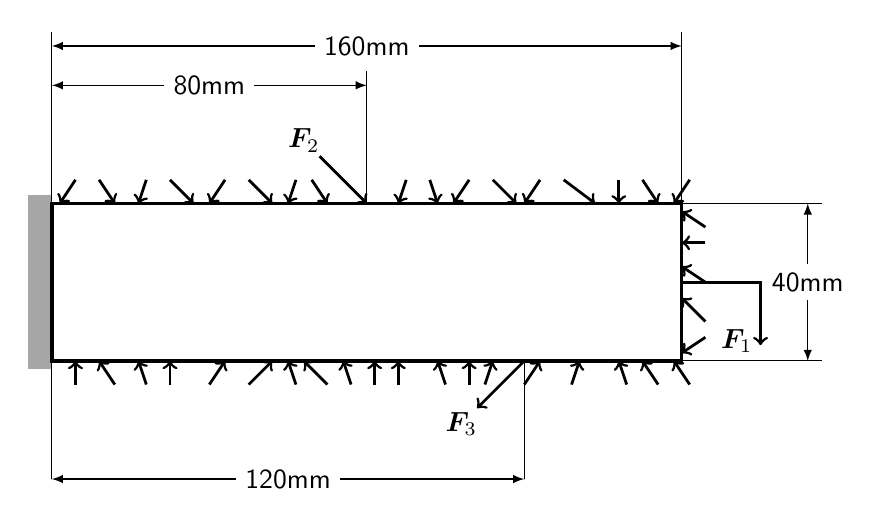
\begin{tikzpicture}
        \draw[fill,color=gray!70] (0,-0.1) rectangle (-0.3,2.1);
        \node [align=center, body,line width=1.2pt,minimum height=2cm,minimum width=8cm,anchor=south west] (body1) at (0,0) {};
        \draw (body1.south east) -- ++(1.6,0) coordinate (D1) -- +(5pt,0);
        \draw (body1.north east) -- ++(1.6,0) coordinate (D2) -- +(5pt,0);
        \draw [dimen] (D1) -- (D2) node {40mm};

        \draw (body1.north west) -- ++(0,2) coordinate (D1) -- +(0,5pt);
        \draw (body1.north east) -- ++(0,2) coordinate (D2) -- +(0,5pt);
        \draw [dimen] (D1) -- (D2) node {160mm};

        \draw[->,line width=1pt] (8,1) -- (9,1) -- (9,0.2);
        \node (arrowhead) at (8.7,0.25) {$\bm{F}_1$};

        \draw (body1.north west) -- ++(0,1.5) coordinate (D1) -- +(0,5pt);
        \draw (4,2) -- ++(0,1.5) coordinate (D2) -- +(0,5pt);
        \draw [dimen] (D1) -- (D2) node {80mm};

        \draw[->,line width=1pt] (3.4,2.6) -- (4,2);
        \node (arrowhead) at (3.2,2.8) {$\bm{F}_2$};

        \draw (body1.south west) -- ++(0,-1.5) coordinate (D1) -- +(0,5pt);
        \draw (6,0) -- ++(0,-1.5) coordinate (D2) -- +(0,5pt);
        \draw [dimen] (D1) -- (D2) node {120mm};

        \draw[->,line width=1pt] (6,0) -- (5.4,-0.6);
        \node (arrowhead) at (5.2,-0.8) {$\bm{F}_3$};

        \draw[->,line width=1pt] (0.3,2.3) -- (0.1,2);
        \draw[->,line width=1pt] (0.6,2.3) -- (0.8,2);
        \draw[->,line width=1pt] (1.2,2.3) -- (1.1,2);
        \draw[->,line width=1pt] (1.5,2.3) -- (1.8,2);
        \draw[->,line width=1pt] (2.2,2.3) -- (2.0,2);
        \draw[->,line width=1pt] (2.5,2.3) -- (2.8,2);
        \draw[->,line width=1pt] (3.1,2.3) -- (3.0,2);
        \draw[->,line width=1pt] (3.3,2.3) -- (3.5,2);
        \draw[->,line width=1pt] (4.5,2.3) -- (4.4,2);
        \draw[->,line width=1pt] (4.8,2.3) -- (4.9,2);
        \draw[->,line width=1pt] (5.3,2.3) -- (5.1,2);
        \draw[->,line width=1pt] (5.6,2.3) -- (5.9,2);
        \draw[->,line width=1pt] (6.2,2.3) -- (6.0,2);
        \draw[->,line width=1pt] (6.5,2.3) -- (6.9,2);
        \draw[->,line width=1pt] (7.2,2.3) -- (7.2,2);
        \draw[->,line width=1pt] (7.5,2.3) -- (7.7,2);
        \draw[->,line width=1pt] (8.1,2.3) -- (7.9,2);

        \draw[->,line width=1pt] (0.3,-0.3) -- (0.3,0);
        \draw[->,line width=1pt] (0.8,-0.3) -- (0.6,0);
        \draw[->,line width=1pt] (1.2,-0.3) -- (1.1,0);
        \draw[->,line width=1pt] (1.5,-0.3) -- (1.5,0);
        \draw[->,line width=1pt] (2.0,-0.3) -- (2.2,0);
        \draw[->,line width=1pt] (2.5,-0.3) -- (2.8,0);
        \draw[->,line width=1pt] (3.1,-0.3) -- (3.0,0);
        \draw[->,line width=1pt] (3.5,-0.3) -- (3.2,0);
        \draw[->,line width=1pt] (3.8,-0.3) -- (3.7,0);
        \draw[->,line width=1pt] (4.1,-0.3) -- (4.1,0);
        \draw[->,line width=1pt] (4.4,-0.3) -- (4.4,0);
        \draw[->,line width=1pt] (5.0,-0.3) -- (4.9,0);
        \draw[->,line width=1pt] (5.3,-0.3) -- (5.3,0);
        \draw[->,line width=1pt] (5.5,-0.3) -- (5.6,0);
        \draw[->,line width=1pt] (6.0,-0.3) -- (6.2,0);
        \draw[->,line width=1pt] (6.6,-0.3) -- (6.7,0);
        \draw[->,line width=1pt] (7.3,-0.3) -- (7.2,0);
        \draw[->,line width=1pt] (7.7,-0.3) -- (7.5,0);
        \draw[->,line width=1pt] (8.1,-0.3) -- (7.9,0);

        \draw[->,line width=1pt] (8.3,0.3) -- (8.0,0.1);
        \draw[->,line width=1pt] (8.3,0.5) -- (8.0,0.8);
        \draw[->,line width=1pt] (8.3,1.0) -- (8.0,1.2);
        \draw[->,line width=1pt] (8.3,1.5) -- (8.0,1.5);
        \draw[->,line width=1pt] (8.3,1.7) -- (8.0,1.9);
    \end{tikzpicture} \newline
  }
  \caption{Cantilever beam problem. $\bm{F}_2$ and $\bm{F}_3$ are at 45 degree angles.}
  \label{fig:CantBeam}
\end{figure}


    The 2D cantilever beam problem shown in Figure \ref{fig:CantBeam} was used to run the experiments. A ground mesh of plane stress quadrilateral elements was used, where each element is a square of side length $1 \text{ mm}$, and a sheet thickness of $1 \text{ mm}$. Linear iso-parametric interpolation functions were used for the field and geometric basis functions. A Young's modulus of 1 MPa and Poisson's ratio of 0.3 were used. Finally, a chequerboard density filter for unstructured meshes was used with a radius of 2 mm \citep{Huang2010a}. A 3D version of the problem above was also solved.

    Three variants of the cantilever beam problem were solved:
    \begin{enumerate}
      \item Minimization of the mean compliance $\mu_C$ subject to a volume constraint with a volume fraction of 0.4,
      \item Minimization of a weighted sum of the mean and standard deviation (mean-std) of the compliance $\mu_C + 2.0 \sigma_C$ subject to a volume constraint with a volume fraction of 0.4, and
      \item Volume minimization subject to a maximum compliance constraint with a compliance threshold of $70000 \text{ Nmm}$.
    \end{enumerate}
    A total of 1000 load scenarios were sampled from:
    \begin{align}
      \bm{f}_i = s_1 \bm{F}_1 + s_2 \bm{F}_2 + s_3 \bm{F}_3 + \frac{1}{R - 3} \sum_{j=4}^{R} s_j \bm{F}_j
    \end{align}
    where $\bm{F}_1$, $\bm{F}_2$ and $\bm{F}_3$ are unit vectors with directions as shown in Figure \ref{fig:CantBeam} and $R$ is an integer greater than or equal to 4. $\bm{F}_2$ and $\bm{F}_3$ are at 45 degrees. $s_1$, $s_2$ and $s_3$ are identically and independently uniformly distributed random variables between -2 and 2. $\bm{F}_j$ for $j$ in $4 \dots R$ are vectors with non-zeros at all the surface degrees of freedom without a Dirichlet boundary condition. The non-zero values are identically and independently normally distributed random variables with mean 0 and standard deviation 1. $s_j$ for $j$ in $4 \dots R$ are also identically and independently normally distributed random variables with mean 0 and standard deviation 1. The same loading scenarios were used for the 3 test problems. Let $\bm{F}$ be the matrix whose columns are the sampled $\bm{f}_i$ vectors. Given the way the loading scenarios have been defined the rank of $\bm{F}$ is almost certainly going to be around $R$.

  \subsection{Software}

    All the topology optimization algorithms described in this chapter were implemented in TopOpt.jl \footnote{https://github.com/JuliaTopOpt/TopOpt.jl} using the Julia programming language \citep{Bezanson2014} for handling generic unstructured, iso-parametric meshes.

  \subsection{Settings}

    The value of $x_{min}$ used was $0.001$ for all problems and algorithms. Penalization was done prior to interpolation to calculate $\bm{\rho}$ from $\bm{x}$. A power penalty function and a regularized Heaviside projection were used. All of the problems were solved using 2 continuation SIMP routines. The first incremented the penalty value from $p = 1$ to $p = 6$ in increments of 0.5. Then the Heaviside projection parameter $\beta$ was incremented from $\beta = 0$ to $\beta = 20$ in increments of 4 keeping the penalty value fixed at 6. An exponentially decreasing tolerance from $1e-3$ to $1e-4$ was used for both continuations. 

    The mean and mean-std compliance minimization SIMP subproblems problems were solved using the method of moving asymptotes (MMA) algorithm \citep{Svanberg1987}. MMA parameters of $s_{init} = 0.5$, $s_{incr} = 1.1$ and $s_{decr} = 0.7$ were used as defined in the MMA paper with a maximum of 1000 iterations for each subproblem. The dual problem of the convex approximation was solved using a log-barrier box-constrained nonlinear optimization solver, where the barrier problem was solved using the nonlinear CG algorithm for unconstrained nonlinear optimization \citep{Nocedal2006} as implemented in Optim.jl \footnote{https://github.com/JuliaNLSolvers/Optim.jl} \citep{KMogensen2018}. The nonlinear CG itself used the line search algorithm from \cite{Hager2006} as implemented in LineSearches.jl \footnote{https://github.com/JuliaNLSolvers/LineSearches.jl}. The stopping criteria used was the one adopted by the KKT solver, IPOPT \citep{Wachter2006}. This stopping criteria is less scale sensitive than the KKT residual as it scales down the residual by a value proportional to the mean absolute value of the Lagrangian multipliers.

\section{Accuracy and speed comparison}

In this section, the accuracy and speed of the approximations proposed are presented and compared to the exact values. A method to boost the accuracy of approximations is also presented and mathematically analyzed. Tables \ref{tab:time_mean} and \ref{tab:time_std} show the values computed for the mean compliance $\mu_C$ and its standard deviation $\sigma_C$ respectively together with the time required to compute their values and gradients using: the naive exact approach and the approximate method with trace or diagonal estimation using 100 Rademacher-distributed or Hadamard basis probing vectors. A value of $R = 10$ was used.
\begin{table}
 \centering
 \caption{The table shows the function values of $\mu_C$ computed using the exact method and the approximate method of trace estimation with 100 Rademacher-distributed or Hadamard basis probing vectors for a full ground mesh design. The table also shows the time required to compute or approximate $\mu_C$ and its gradient in each case. A value of $R = 10$ was used here.}
 \begin{tabular}{|c|c|c|}
  \hline
  Method & $\mu_C$ (Nmm) & Time (s) \\
  \hline
  \hline
  Naive Exact & 3328.7 & 24.2 \\
  \hline
  Trace estimation & 3596.9 (Rademacher) / 3486.7 (Hadamard) & 2.6 \\
  \hline
 \end{tabular}
 \label{tab:time_mean}
\end{table}

\begin{table}
 \centering
 \caption{The table shows the function values of $\sigma_C$ and its gradients for a full ground mesh computed using the exact method and the approximate method of diagonal estimation with 100 Rademacher-distributed or Hadamard basis probing vectors. The table also shows the time required to compute the exact or approximate $\sigma_C$ and its gradient in each case. A value of $R = 10$ was used here. Note the extreme bias in the estimate so a correction step is necessary.}
 \begin{tabular}{|c|c|c|}
  \hline
  Method & $\sigma_C$ (Nmm) & Time (s) \\
  \hline
  \hline
  Exact & 4172.8 & 28.0 \\
  \hline
  Diagonal estimation & 9774.8 (Rademacher) / 10173.3 (Hadamard) & 5.2 \\
  \hline
 \end{tabular}
 \label{tab:time_std}
\end{table}

\begin{figure}
  \begin{subfigure}[t]{0.45\textwidth}
    \centering
    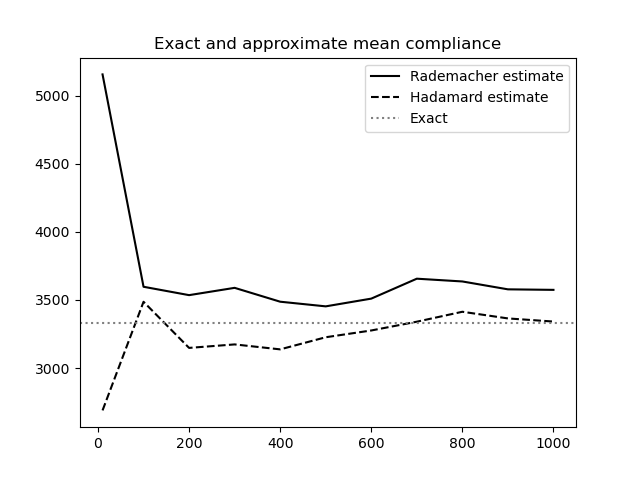
\includegraphics[width=1\textwidth]{./images/robust_approx/exact_approx_mean.png}
    \caption{Mean compliance estimate using different numbers of probing vectors in the trace estimation method.}
    \label{fig:exact_approx_mean}
  \end{subfigure} \hfill
  \begin{subfigure}[t]{0.45\textwidth}
    \centering
    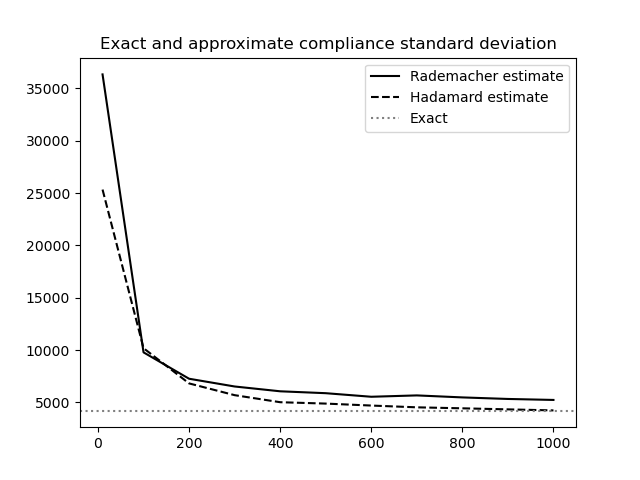
\includegraphics[width=1\textwidth]{./images/robust_approx/exact_approx_std.png}
    \caption{Compliance standard deviation estimate using different numbers of probing vectors in the diagonal estimation method.}
    \label{fig:exact_approx_std}
  \end{subfigure}
  \caption{Accuracy profile of the trace and diagonal estimation methods for estimating the mean compliance and its standard deviation using 10, 100, 200, 300, 400, 500, 600, 700, 800, 900 and 1000 probing vectors. A value of $R = 10$ was used here.}
  \label{fig:exact_approx}
\end{figure}

As expected, the proposed approximation methods take a fraction of the time it takes to compute the exact mean and mean-std compliances using the approaches. Estimates of the mean compliance and its standard deviation for a full ground mesh using different numbers of Rademacher-distributed and Hadamard basis probing vectors are shown in Figure \ref{fig:exact_approx}. In this case, the estimates obtained using the Hadamard basis were always closer to the exact value than that of the Rademacher-distributed one. However, this depends on the order by which the Hadamard basis vectors are used.

\section{Bias correction}

While the Hadamard estimate is converging faster to the exact value compared to the Rademacher one in the above case as the number of probing vectors increases, it is still quite far in the case of the standard deviation unless a large number ofIf we have a constraint over the weighted sum of the mean compliance and its standard deviation, this huge discrepancy from the exact quantity renders the approximate method useless. In this section, it will be shown that usually the estimate can be multiplied by a correcting factor to significantly improve its accuracy. This will be demonstrated experimentally and then mathematically analyzed. When performing topology optimization, the function value and its gradient need to be computed repeatedly. So if we only need to compute the correcting factor a few times, we can still save a lot of computational time when using the approximate method without losing too much accuracy.

\subsection{Experiments}

Using a full ground mesh to calculate the correcting factor and only 10 probing vectors and $R = 10$, the ratio between the exact mean compliance and the trace estimate using Hadamard basis probing vectors was 1.238. Similarly, the ratio of the exact compliance standard deviation to the estimated value was 0.165. Figures \ref{fig:correcting_mean} and \ref{fig:correcting_std} show the distributions of the ratios of the exact value to the estimated one for the mean compliance and its standard deviation respectively. The same 10 Hadamard basis probing vectors were used and each figure was generated using 500 random designs. For each figure, the random designs were sampled from a truncated normal distributions with a different mean and a standard deviation of 0.2, truncated between 0 and 1. One can see that using the same probing vectors, the ratio between the exact and estimated values doesn't change significantly even when changing the mean volume by changing the mean of the truncated normal distribution. One can see that the correcting ratio that can multiply the estimated mean compliance or standard deviation to get the exact one is not very sensitive to the underlying design.

\begin{figure}[!htbp]
  \begin{subfigure}{0.45\textwidth}
    \centering
    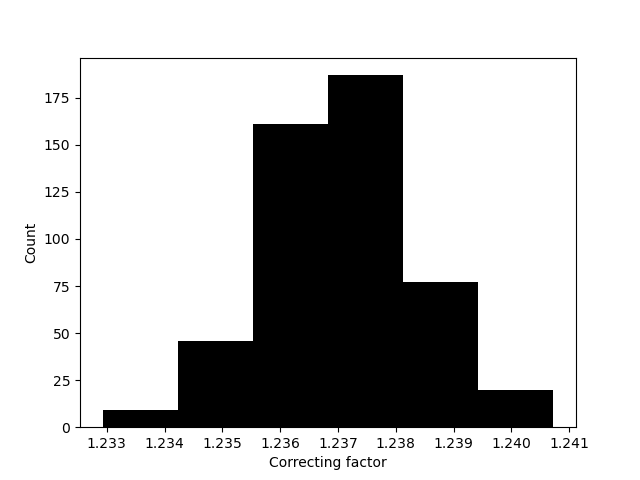
\includegraphics[width=1\textwidth]{./images/robust_approx/correcting_factors_hadamard_mean_10_01.png}
    \caption{Mean = 0.1}
  \end{subfigure}
  \begin{subfigure}{0.45\textwidth}
    \centering
    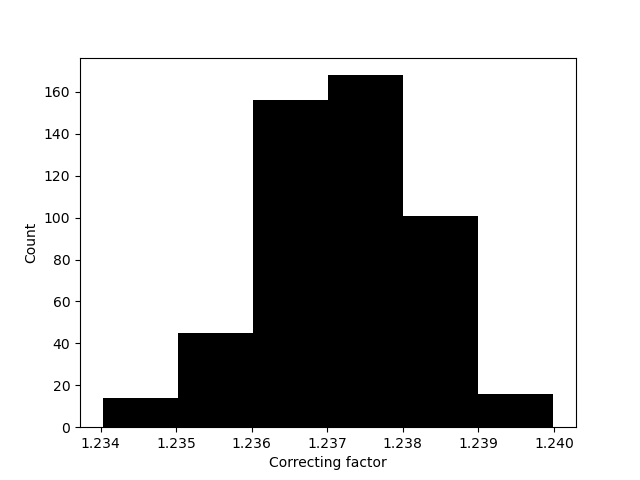
\includegraphics[width=1\textwidth]{./images/robust_approx/correcting_factors_hadamard_mean_10_03.png}
    \caption{Mean = 0.3}
  \end{subfigure}
  \begin{subfigure}{0.45\textwidth}
    \centering
    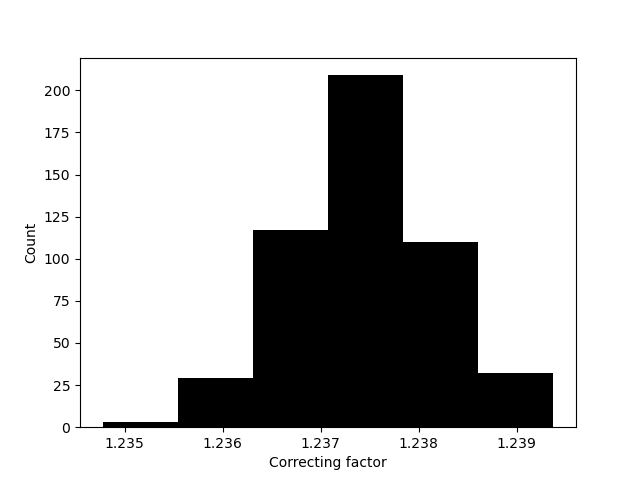
\includegraphics[width=1\textwidth]{./images/robust_approx/correcting_factors_hadamard_mean_10_05.png}
    \caption{Mean = 0.5}
  \end{subfigure} 
  \begin{subfigure}{0.45\textwidth}
    \centering
    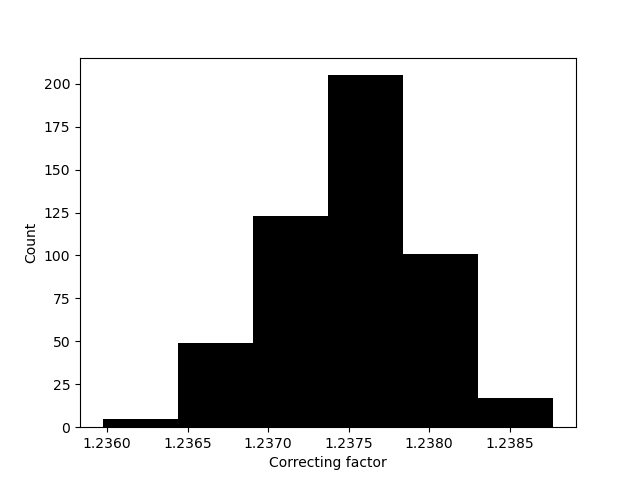
\includegraphics[width=1\textwidth]{./images/robust_approx/correcting_factors_hadamard_mean_10_07.png}
    \caption{Mean = 0.7}
  \end{subfigure} 
  \begin{subfigure}{0.45\textwidth}
    \centering
    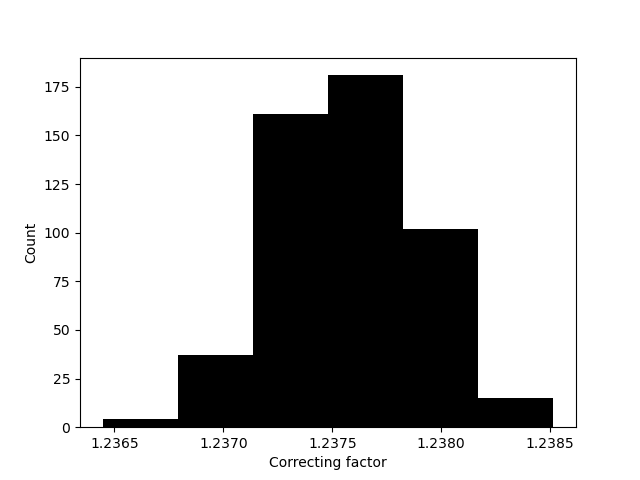
\includegraphics[width=1\textwidth]{./images/robust_approx/correcting_factors_hadamard_mean_10_09.png}
    \caption{Mean = 0.9}
  \end{subfigure}
  \caption{Histograms of the ratio between the exact mean compliance and the trace estimate using 10 Hadamard basis probing vectors. In each figure, 500 designs were randomly sampled where each element's pseudo-density is sampled from a truncated normal distribution with the means indicated above and a standard deviation of 0.2, truncated between 0 and 1. A value of $R = 10$ was used here.}
  \label{fig:correcting_mean}
\end{figure}
\begin{figure}[!htbp]
  \begin{subfigure}[t]{0.45\textwidth}
    \centering
    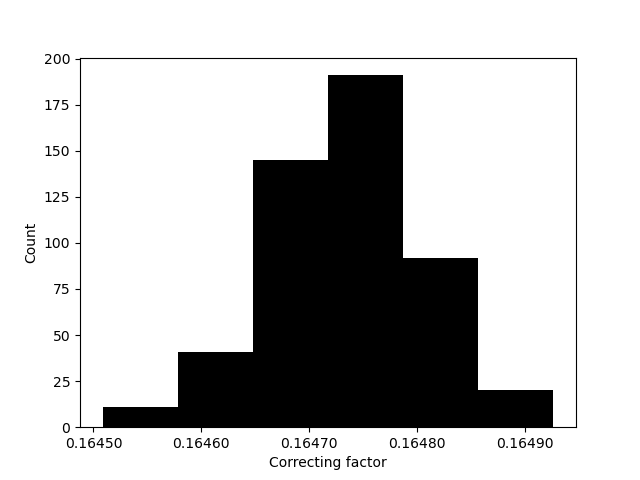
\includegraphics[width=1\textwidth]{./images/robust_approx/correcting_factors_hadamard_std_10_01.png}
    \caption{Mean = 0.1}
  \end{subfigure}
  \begin{subfigure}[t]{0.45\textwidth}
    \centering
    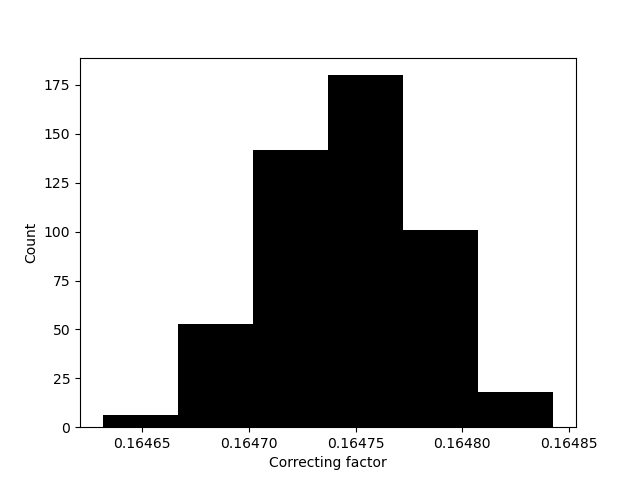
\includegraphics[width=1\textwidth]{./images/robust_approx/correcting_factors_hadamard_std_10_03.png}
    \caption{Mean = 0.3}
  \end{subfigure}
  \begin{subfigure}[t]{0.45\textwidth}
    \centering
    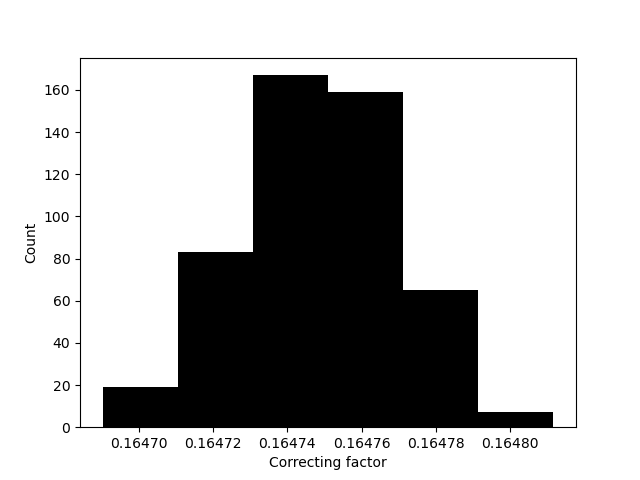
\includegraphics[width=1\textwidth]{./images/robust_approx/correcting_factors_hadamard_std_10_05.png}
    \caption{Mean = 0.5}
  \end{subfigure}
  \begin{subfigure}[t]{0.45\textwidth}
    \centering
    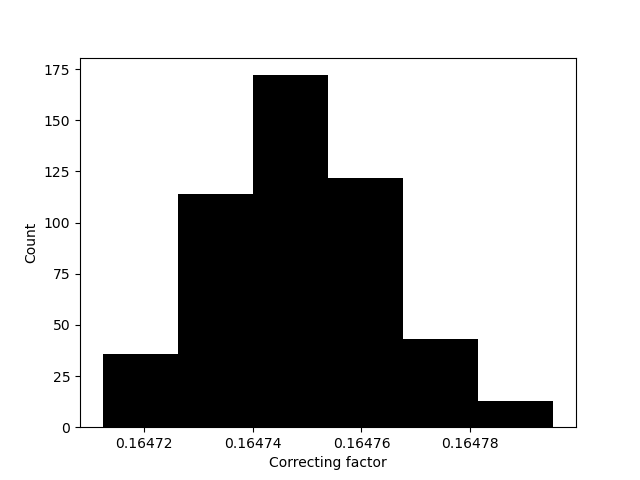
\includegraphics[width=1\textwidth]{./images/robust_approx/correcting_factors_hadamard_std_10_07.png}
    \caption{Mean = 0.7}
  \end{subfigure}
  \begin{subfigure}[t]{0.45\textwidth}
    \centering
    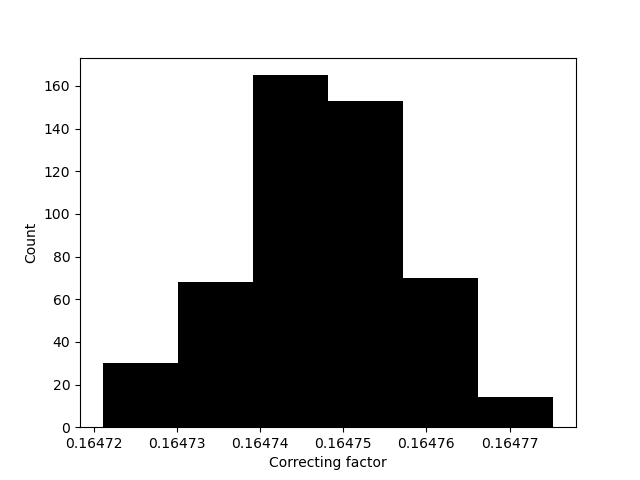
\includegraphics[width=1\textwidth]{./images/robust_approx/correcting_factors_hadamard_std_10_09.png}
    \caption{Mean = 0.9}
  \end{subfigure}
  \caption{Histograms of the ratio between the exact compliance standard deviation and the estimate using 10 Hadamard basis probing vectors. In each figure, 500 designs were randomly sampled where each element's pseudo-density is sampled from a truncated normal distribution with the means indicated above and a standard deviation of 0.2, truncated between 0 and 1. A value of $R = 10$ was used here.}
  \label{fig:correcting_std}
\end{figure}

\subsection{Mathematical analysis} \label{sec:analysis}

In this section, an attempt will be made to mathematically explain the insensitivity of the estimators' correcting ratios to the design as shown above. While this section doesn't provide a rigorous proof of the phenomena observed, it does provide some mathematical insight into why it is happening and when it can be expected to happen in other problems.

Let the diagonal estimator be:
\begin{align}
\frac{1}{N} \sum_{k = 1}^N \bm{D}_{\bm{v}_k} \bm{A} \bm{v}_k = 
\frac{1}{N} \Bigl(\sum_{k = 1}^N \bm{D}_{\bm{v}_k} \bm{A} \bm{D}_{\bm{v}_k} \Bigr) \bm{1}
\end{align}
where $\bm{A} = \bm{F}^T \bm{K}^{-1} \bm{F}$. Let $a_{ij}$ be $(i,j)^{th}$ element of $\bm{A}$. Let $v_{ki}$ be the $i^{th}$ element of $\bm{v}_k$. The $(i,j)^{th}$ element of $\sum_{k = 1}^N \bm{D}_{\bm{v}_k} \bm{A} \bm{D}_{\bm{v}_k}$ is therefore $a_{ij} \sum_{k=1}^N v_{ki}v_{kj}$. Let $N^+_{ij}$ be the number of times $v_{ki}v_{kj}$ is 1 and $N^-_{ij}$ be the number of times $v_{ki}v_{kj}$ is -1. In the case of Hadamard basis, if $N$ is the smallest power of 2 larger than or equal to the number of loads $L$, then:
\begin{align}
  N^+_{ij} = N^-_{ij} = N/2 & \quad \textit{if} \quad i \neq j \\
  N^+_{ij} = N, N^-_{ij} = 0 & \quad \textit{if} \quad i = j
\end{align}
This means that the diagonal estimate will be exact in that case. Bekas et al. \cite{Bekas2007} showed that Hadamard basis work well for banded matrices and for matrices where off-diagonal values are decaying rapidly away from the diagonal. However in the case of load compliances, neither of those conditions apply. Therefore, as shown in the experiment above, the accuracy of the estimated diagonal is quite bad as obvious from the standard deviation of the estimate. Let the $i^{th}$ diagonal element (or load compliance) be $C_i = a_{ii}$. The estimator of $a_{ii}$, $\hat{a}_{ii}$, can be written as:
\begin{align}
  \hat{a}_{ii} & = \frac{1}{N} \sum_{j=1}^L a_{ij} \sum_{k=1}^N v_{ki}v_{kj} \\
  & = \frac{1}{N} \sum_{j=1}^L a_{ij} (N^+_{ij} - N^-_{ij}) \\
  & = a_{ii} + \sum_{j \neq i} a_{ij} \frac{N^+_{ij} - N^-_{ij}}{N}
\end{align}
The ratio of the estimated diagonal element to the actual diagonal element is:
\begin{align}
  \frac{\hat{a}_{ii}}{a_{ii}} = 1 + \sum_{j \neq i} \frac{a_{ij}}{a_{ii}} \frac{N^+_{ij} - N^-_{ij}}{N}
\end{align}
This ratio depends on:
\begin{enumerate}
  \item $\frac{a_{ij}}{a_{ii}}$ which depends on the design and the load scenarios, and
  \item $N^+_{ij}$ and $N^-_{ij}$ which depend on the Hadamard basis used. 
\end{enumerate}
If the same basis are used for all the designs during optimization, then $\frac{a_{ij}}{a_{ii}}$ is the only number that can vary.
\begin{align}
  \frac{a_{ij}}{a_{ii}} = \frac{\bm{f}_i^T \bm{K}^{-1} \bm{f}_j}{\bm{f}_i^T \bm{K}^{-1} \bm{f}_i}
\end{align}
The partial derivative of $a_{ij} / a_{ii}$ with respect to the $e^{th}$ element's density $\rho_e$ is:
\begin{align}
  \frac{\partial (a_{ij} / a_{ii})}{\partial \rho_e} & = \frac{\partial (\bm{f}_i^T \bm{K}^{-1} \bm{f}_j / \bm{f}_i^T \bm{K}^{-1} \bm{f}_i)}{\partial \rho_e} \\
  & = \frac{\frac{\partial \bm{f}_i^T \bm{K}^{-1} \bm{f}_j}{\partial \rho_e} \bm{f}_i^T \bm{K}^{-1} \bm{f}_i - \frac{\partial \bm{f}_i^T \bm{K}^{-1} \bm{f}_i}{\partial \rho_e} \bm{f}_i^T \bm{K}^{-1} \bm{f}_j}{(\bm{f}_i^T \bm{K}^{-1} \bm{f}_i)^2} \\
  & = \frac{-(\bm{u}_i^T \bm{K}_e \bm{u}_j) (\bm{u}_i^T \bm{K} \bm{u}_i) + (\bm{u}_i^T \bm{K}_e \bm{u}_i) (\bm{u}_i^T \bm{K} \bm{u}_j)}{(\bm{u}_i^T \bm{K} \bm{u}_i)^2} \\
  %& = \frac{1}{2} \frac{(\bm{u}_i + \bm{u}_j)^T \bm{K}_e (\bm{u}_i + \bm{u}_j) - \bm{u}_i^T \bm{K}_e \bm{u}_i - \bm{u}_j^T \bm{K}_e \bm{u}_j}{\bm{u}_i^T \bm{K} \bm{u}_i} + \\
  %& \frac{\bm{u}_i^T \bm{K}_e \bm{u}_i}{2\bm{u}_i^T \bm{K} \bm{u}_i} \frac{(\bm{u}_i + \bm{u}_j)^T \bm{K} (\bm{u}_i + \bm{u}_j) - \bm{u}_i^T \bm{K} \bm{u}_i - \bm{u}_j^T \bm{K} \bm{u}_j}{\bm{u}_i^T \bm{K} \bm{u}_i}
\end{align}

\begin{lemma}
  \begin{align}
    |\bm{u}_i^T \bm{K} \bm{u}_j| \leq \frac{1}{2} \max(|(\bm{u}_i + \bm{u}_j)^T \bm{K} (\bm{u}_i + \bm{u}_j)|, |\bm{u}_i^T \bm{K} \bm{u}_i + \bm{u}_j^T \bm{K} \bm{u}_j|)
  \end{align}
  if $\bm{K}$ is positive or negative semi-definite and
  \begin{align}
    |\bm{u}_i^T \bm{K} \bm{u}_j| \leq \frac{1}{2} \Big( |(\bm{u}_i + \bm{u}_j)^T \bm{K} (\bm{u}_i + \bm{u}_j)| + |\bm{u}_i^T \bm{K} \bm{u}_i| + |\bm{u}_j^T \bm{K} \bm{u}_j)| \Big)
  \end{align}
  otherwise.
  \label{lemma:bound1}
\end{lemma}
\begin{proof}
  \begin{align}
    2 \bm{u}_i^T \bm{K} \bm{u}_j = (\bm{u}_i + \bm{u}_j)^T \bm{K} (\bm{u}_i + \bm{u}_j) - \bm{u}_i^T \bm{K} \bm{u}_i - \bm{u}_j^T \bm{K} \bm{u}_j
  \end{align}
  If $\bm{K}$ is indefinite:
  \begin{align}
    2 |\bm{u}_i^T \bm{K} \bm{u}_j| \leq |(\bm{u}_i + \bm{u}_j)^T \bm{K} (\bm{u}_i + \bm{u}_j)| + |\bm{u}_i^T \bm{K} \bm{u}_i| + |\bm{u}_j^T \bm{K} \bm{u}_j|
  \end{align}
  If $\bm{K}$ is positive semi-definite, then $(\bm{u}_i + \bm{u}_j)^T \bm{K} (\bm{u}_i + \bm{u}_j)$, $\bm{u}_i^T \bm{K} \bm{u}_i$ and $\bm{u}_j^T \bm{K} \bm{u}_j$ are all non-negative. Therefore:
  \begin{align}
    -(\bm{u}_i^T \bm{K} \bm{u}_i + \bm{u}_j^T \bm{K} \bm{u}_j) \leq 2 \bm{u}_i^T \bm{K} \bm{u}_j \leq (\bm{u}_i + \bm{u}_j)^T \bm{K} (\bm{u}_i + \bm{u}_j)
  \end{align}
  Similarly, if $\bm{K}$ is negative semi-definite, then \\ $(\bm{u}_i + \bm{u}_j)^T \bm{K} (\bm{u}_i + \bm{u}_j)$, $\bm{u}_i^T \bm{K} \bm{u}_i$ and $\bm{u}_j^T \bm{K} \bm{u}_j$ are all non-positive. Therefore:
  \begin{align}
    (\bm{u}_i + \bm{u}_j)^T \bm{K} (\bm{u}_i + \bm{u}_j) \leq 2 \bm{u}_i^T \bm{K} \bm{u}_j \leq -(\bm{u}_i^T \bm{K} \bm{u}_i + \bm{u}_j^T \bm{K} \bm{u}_j)
  \end{align}
  It follows that:
  \begin{align}
    2 |\bm{u}_i^T \bm{K} \bm{u}_j| \leq \max(|(\bm{u}_i + \bm{u}_j)^T \bm{K} (\bm{u}_i + \bm{u}_j)|, |\bm{u}_i^T \bm{K} \bm{u}_i + \bm{u}_j^T \bm{K} \bm{u}_j|)
  \end{align}
  This completes the proof.
\end{proof}
Using the above bound, it follows that if for all combinations of $i$ and $j$:
\begin{align}
  \frac{\bm{u}_j^T \bm{K}_e \bm{u}_j}{\bm{u}_i^T \bm{K} \bm{u}_i} \leq \alpha_1 \\
  \frac{(\bm{u}_i + \bm{u}_j)^T \bm{K}_e (\bm{u}_i + \bm{u}_j)}{2 \bm{u}_i^T \bm{K} \bm{u}_i} \leq \beta_1 \\
  \frac{\bm{u}_j^T \bm{K} \bm{u}_j}{\bm{u}_i^T \bm{K} \bm{u}_i} \leq \alpha_2\\
  \frac{(\bm{u}_i + \bm{u}_j)^T \bm{K} (\bm{u}_i + \bm{u}_j)}{2 \bm{u}_i^T \bm{K} \bm{u}_i} \leq \beta_2
\end{align}
then
\begin{align}
  \Bigl|\frac{\partial (a_{ij} / a_{ii})}{\partial \rho_e}\Bigr| & \leq \max(\alpha_1, \beta_1) + \alpha_1 \times \max(\alpha_2, \beta_2)
\end{align}
It is natural to expect $\alpha_1$ to be small since the element compliance due to any one load will likely be much smaller than the total compliance due to any other load. If the loading scenarios have widely varying magnitudes, $\alpha_1$ may be large in that case. However to remedy this, the loading scenarios can be clustered into groups by their norm and a separate estimator can be used for each group. Similarly, $\beta_1$ is likely to be small if all the forces have a close enough norm since the element compliance due to the superposition of 2 loads is likely to be much smaller than two times the total compliance due to any other load. If the norms of the loads are somewhat similar, $\alpha_2$ and $\beta_2$ can also be expected to be small constants greater than or equal to 1. This means that absolute value of the individual partial derivatives can be upper bounded by a small positive number. Interestingly, the sum of all the partial derivatives of the correcting ratio with respect to the individual element densities, $\sum_e \frac{\partial (a_{ij} / a_{ii})}{\partial \rho_e}$, is 0. This does not guarantee that the directional derivative in any direction will be small but it increases the chances of term cancellation. This is consistent with the observations.

However, the correcting factor for the estimator $\hat{C}_i = \hat{a}_{ii}$ does not just depend on the individual $\frac{\partial (a_{ij} / a_{ii})}{\partial \rho_e}$ but rather it depends on the sum $\sum_{j \neq i} \frac{a_{ij}}{a_{ii}} \frac{N^+_{ij} - N^-_{ij}}{N}$. Three factors can make this sum small:
\begin{enumerate}
  \item A good choice of probing vectors that make the distribution of $N^+_{ij} - N^-_{ij}$ for different $(i,j)$ pairs symmetric around 0 promoting term cancellation.
  \item Term cancellation due to the alternating signs of $a_{ij}$. For instance if the mean load vector is the $\bm{0}$ vector, the summation $\sum_{j \neq i} \frac{a_{ij}}{a_{ii}}$ is equal to -1 regardless of the number of loading scenarios.
  \item A small ratio of the number of loading scenarios to the number of elements. This is detailed below.
\end{enumerate}
For fixed loading scenarios, the values of $\alpha_1$ and $\beta_1$ decrease as the number of elements $E$ increases. This is because the ratio of an individual element's contribution to the total strain energy decreases as the element size decreases. Given that $-1 \leq \frac{N^+_{ij} - N^-_{ij}}{N} \leq 1$:
\begin{align}
  \Biggl|\sum_{j \neq i} \frac{a_{ij}}{a_{ii}} \frac{N^+_{ij} - N^-_{ij}}{N} \Biggr| \leq (L - 1)(\beta_1 + \alpha_1 + \alpha_1 (\beta_2 + \alpha_2))
\end{align}
Therefore, if $L \ll E$ and the loads in $\bm{F}$ have close magnitudes, one can expect the correcting factor to be design insensitive especially near the end of the optimization when the design is not changing much. 

The analysis above identified 3 strategies other than using more probing vectors that can help promote the insensitivity of the correcting factors to the design:
\begin{enumerate}
  \item Clustering the loads by their magnitudes with a maximum number of loads per cluster $\ll E$,
  \item Centering the loads around $\bm{0}$. Let $\bm{\mu}_{\bm{f}}$ be the sample mean of the loading scenarios and let $\tilde{\bm{f}}_i = \bm{f}_i - \bm{\mu}_{\bm{f}}$. The $i^{th}$ load compliance $\bm{f}_i^T \bm{K}^{-1} \bm{f}_i$ would then be $\tilde{\bm{f}}_i^T \bm{K}^{-1} \tilde{\bm{f}}_i + 2 \tilde{\bm{f}}_i^T \bm{K}^{-1} \bm{\mu}_{\bm{f}} + \bm{\mu}_{\bm{f}}^T \bm{K}^{-1} \bm{\mu}_{\bm{f}}$. The terms $\tilde{\bm{f}}_i^T \bm{K}^{-1} \tilde{\bm{f}}_i$ can be obtained from the diagonal estimator of $\tilde{\bm{F}}^T \bm{K}^{-1} \tilde{\bm{F}}$ where the columns of $\tilde{\bm{F}}$ are the vectors $\tilde{\bm{f}}_i$. The remaining terms can be computed using a single linear system solve $\bm{K}^{-1} \bm{\mu}_{\bm{f}}$.
  \item Using a finer mesh, i.e. increasing $E$ thus decreasing $\alpha_1$ and $\beta_1$.
\end{enumerate}

Note that while the analysis above provides some mathematical insights into why the correcting ratios for the individual compliances may not be sensitive to the design, it is not a complete proof of the phenomena observed because only a single element's $\rho_e$ was assumed to be changing in the analysis. However, from the analysis above one can see that term cancellation is highly likely in practice. For instance, the sum of $\frac{a_{ij}}{a_{ii}}$ for all $j$ is equal to -1 if the mean load is $\bm{0}$ regardless of the number of loads, and the sum of $\frac{\partial a_{ij}/a_{ii}}{\partial \rho_e}$ for all $e$ is equal to 0. This term cancellation is the main reason behind the extreme insensitivity of the correcting ratio to the design observed in the experiments above even when all the elements' densities are changing in random directions by large amounts.

Next it will be shown that under some conditions that the above insensitivity of the correcting ratio to any individual $\rho_e$ can be extended to a class of scalar-valued functions of the load compliances. This class of functions includes the mean, variance and standard deviation but not the augmented Lagrangian penalty. Let $\gamma_i$ be the correcting factor for the compliance $C_i$. The correcting factor of a scalar valued function $f$ of the load compliances can therefore be written as:
\begin{align}
  \eta(\bm{\rho}) = \frac{f(\gamma_1(\bm{\rho}) \hat{C}_1(\bm{\rho}), \gamma_2(\bm{\rho}) \hat{C}_2(\bm{\rho}), \dots, \gamma_L(\bm{\rho}) \hat{C}_L(\bm{\rho}))}{f(\hat{C}_1(\bm{\rho}), \hat{C}_2(\bm{\rho}), \dots, \hat{C}_L(\bm{\rho}))}
\end{align}
Let $f_{\bm{\hat{C}}} = f(\hat{C}_1, \dots, \hat{C}_L)$ and $f_{\bm{C}} = f(\gamma_1 \hat{C}_1, \dots, \gamma_L \hat{C}_L)$. Furthermore, let $f_{\bm{\hat{C}}}^{(i)}$ be the partial derivative of $f$ with respect to its $i^{th}$ argument evaluated at $(\hat{C}_1, \hat{C}_2, \dots, \hat{C}_L)$ and let $f_{\bm{C}}^{(i)}$ be the partial derivative of $f$ with respect to its $i^{th}$ argument evaluated at $(\gamma_1 \hat{C}_1, \gamma_2 \hat{C}_2, \dots, \gamma_L \hat{C}_L)$.
\begin{align}
  \frac{\partial \eta}{\partial \rho_e} & 
  = \sum_i \Biggl(\frac{\partial \eta}{\partial \gamma_i} * \frac{\partial \gamma_i}{\partial \rho_e} + 
  \frac{\partial \eta}{\partial \hat{C}_i} * \frac{\partial \hat{C}_i}{\partial \rho_e}\Biggr) \\
  & = \sum_i \Biggl( \frac{f_{\bm{C}}^{(i)} \hat{C}_i}{f_{\hat{\bm{C}}}} \frac{\partial \gamma_i}{\partial \rho_e} + \Biggl( \frac{f_{\bm{C}}^{(i)} \gamma_i}{f_{\bm{\hat{C}}}} - \frac{f_{\bm{\hat{C}}}^{(i)} f_{\bm{C}}}{f_{\hat{\bm{C}}}^2} \Biggr) \frac{\partial \hat{C}_i}{\partial \rho_e} \Biggr)
\end{align}
One can see that if the magnitudes of $f_{\hat{\bm{C}}}^{(i)}$ and $f_{\bm{C}}^{(i)}$ scale down as $L$ increases and if $f_{\bm{C}} / f_{\hat{\bm{C}}}^2$ is small that the partial derivative $\frac{\partial \eta}{\partial \rho_e}$ will also likely be small. For all $i$, let:
\begin{align}
  |f_{\bm{C}}^{(i)}| \leq \frac{c_1}{L} \\
  |f_{\hat{\bm{C}}}^{(i)}| \leq \frac{c_1}{L} \\
  \Bigl| \frac{\partial \hat{C}_i}{\partial \rho_e} \Bigr| \leq c_2 \\
  \Bigl| \frac{\partial \gamma_i}{\partial \rho_e} \Bigr| \leq c_3 \\
  \Bigl| \frac{\hat{C}_i}{f_{\hat{\bm{C}}}} \Bigr| \leq c_4 \\
  \Bigl| \frac{\gamma_i}{f_{\hat{\bm{C}}}} \Bigr| \leq c_5 \\
  \Bigl| \frac{f_{\bm{C}}}{f_{\hat{\bm{C}}}^2} \Bigr| \leq c_6
\end{align}
Then one can set the bound:
\begin{align}
  \Biggl| \frac{\partial \eta}{\partial \rho_e} \Biggr| \leq c_1 c_4 c_3 + c_1 c_5 c_2 + c_1 c_6 c_2
\end{align}
From the above bound, one can see that $c_3$, $c_5$ and $c_6$ must be small enough to guarantee a low upper bound on the absolute value of $\frac{\partial \eta}{\partial \rho_e}$. This means that:
\begin{enumerate}
  \item The diagonal's correcting factors must not be sensitive to $\rho_e$ (i.e. $c_3$ is small). This has been established above under some conditions.
  \item The ratio of the diagonal correcting factors to the function estimator $f_{\hat{\bm{C}}}$ must be small in magnitude, i.e. ($c_5$ is small). This is true for the experiment above, where the diagonal correcting ratios at the full ground mesh ranged from -19.0 to 21.7 while the estimated compliance mean and standard deviation were 410.0 and 1329.7 respectively.
  \item The ratio $f_{\bm{C}} / f_{\hat{\bm{C}}}^2$ must be small in magnitude, (i.e. $c_6$ is small). This is also true for the experiment above at the full ground mesh where the ratios were $2.7e-3$ and $3.0e-4$ for the mean and standard deviation of the compliance respectively.
\end{enumerate}

To show that the above result applies to the mean, standard deviation and variance functions, it suffices to show that $|f_{\bm{C}}^{(i)}| \leq \frac{c_1}{L}$ for some constant $c_1$. If this is true for $f_{\bm{C}}^{(i)}$ then it is also true for $f_{\hat{\bm{C}}}^{(i)}$ since this is the same function evaluated at different points. The partial derivatives of the mean, standard deviation and variance of $(C_1, C_2, \dots, C_L)$ with respect to each $C_i$ are:
\begin{align}
    \frac{\partial \mu_C}{\partial C_i} = \frac{1}{L}
\end{align}
\begin{align}
    \frac{\partial \sigma_C}{\partial C_i} = \Big( 1 - \frac{1}{L} \Big) \frac{C_i - \mu_C}{(L - 1) \times \sigma_C} \leq \frac{2(C_i - \mu_C)}{L \times \sigma_C}
\end{align}
\begin{align}
    \frac{\partial \sigma_C^2}{\partial C_i} = \Big( 1 - \frac{1}{L} \Big) \frac{2(C_i - \mu_C)}{(L - 1)} \leq \frac{4(C_i - \mu_C)}{L}
\end{align}
because $L - 1 \geq L / 2$ for $L > 1$. Let $l_{\mu_C}$ and $l_{\sigma_C}$ be lower bounds on $\mu_C$ and $\sigma_C$ for all the designs. The constant $c_1$ is therefore $1$ for $\mu_C$, $2(C_{max} - l_{\mu_C})/l_{\sigma_C}$ for $\sigma_C$ and $4(C_{max} - l_{\mu_C})$ for $\sigma_C^2$.

Finally for the augmented Lagrangian function, it was not possible to establish the bound above. Even if the compliance constraints were scaled by $1/L$ allowing a bound of the form $c_1 / L$, $c_1$ would still scale up with the linear and quadratic penalties of the augmented Lagrangian function. The linear penalty is unbounded from above and the quadratic penalty grows exponentially during the optimization process. This means that no tight bound can be established. The experiments run were also consistent with this result where the diagonal estimation method was found to not work when solving a maximum compliance constrained problem using the augmented Lagrangian algorithm. A meaningless design was produced.

\section{Optimization}

\subsection{Low rank loads}

When minimizing the mean compliance only, the insensitivity of the correcting ratio to the design implies that one can minimize the mean compliance estimate instead of the exact one and get a reasonable design. This will be demonstrated in this section. In this section, a rank $R = 10$ is used and the trace estimation method is compared against the naive exact method where all the loading scenarios are enumerated. When minimizing the weighted sum of the mean and standard deviation of the compliance, a corrected estimator was used by calculating the correcting ratio of the mean and standard deviation estimators separately at the full ground mesh. Let the uncorrected mean compliance estimator be $\hat{\mu}_C$ and the uncorrected standard deviation estimator be $\hat{\sigma}_C$. The corrected estimator, $\hat{W}$, of the weighted sum of the mean and standard deviation used was:
\begin{align} \label{eqn:corrected_estimator}
 \hat{W} = \frac{\mu_C(\bm{x}_0)}{\hat{\mu}_C(\bm{x}_0)} \hat{\mu}_C(\bm{x}) + 2 \frac{\sigma_C(\bm{x}_0)}{\hat{\sigma}_C(\bm{x}_0)} \hat{\sigma}_C(\bm{x})
\end{align}
Only Hadamard basis probing vectors were used in this section.

\subsubsection{Mean compliance minimization}

To demonstrate the effectiveness of the proposed approaches, the cantilever beam problem described in section \ref{sec:exp_impl} was solved using the proposed exact and approximate methods. Table \ref{tab:mean_stats} shows the statistics of the final optimal solutions obtained by minimizing the mean compliance subject to the volume fraction constraint using exact and trace estimation methods to evaluate the mean compliance. 10 Hadamard basis probing vectors were used in the trace estimator. The optimal topologies are shown in Figure \ref{fig:mean}.

While the designs obtained were different, both algorithms converged to reasonable designs in similar amounts of time. The convergence time shows that the convergence behavior was not affected by the use of an estimator in place of the original objective. However, the design produced by the trace estimation method was significantly worse than the exact method's which is to be expected since an approximate objective was minimized. Finally, note that the correcting ratio of the mean compliance estimator at the final design is 1.276 which is very close to the values shown in Figure \ref{fig:correcting_mean}.

\begin{figure}
  \begin{subfigure}[t]{0.8\textwidth}
    \centering
    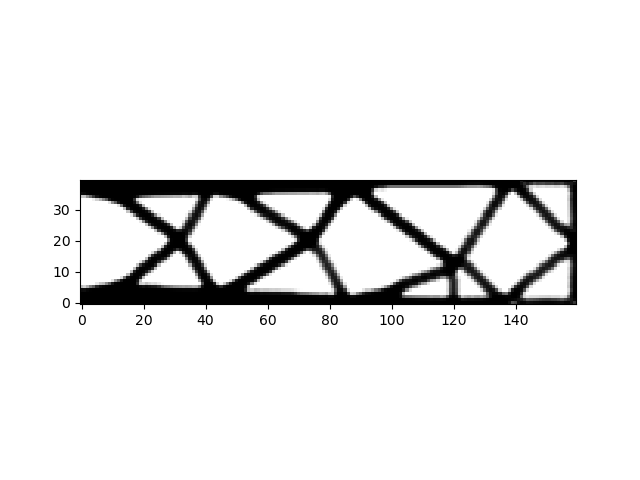
\includegraphics[width=1\textwidth]{./images/robust_approx/exact_svd_mean_csimp.png}
    \caption{Exact method.}
  \end{subfigure} \hfill
  \begin{subfigure}[t]{0.8\textwidth}
    \centering
    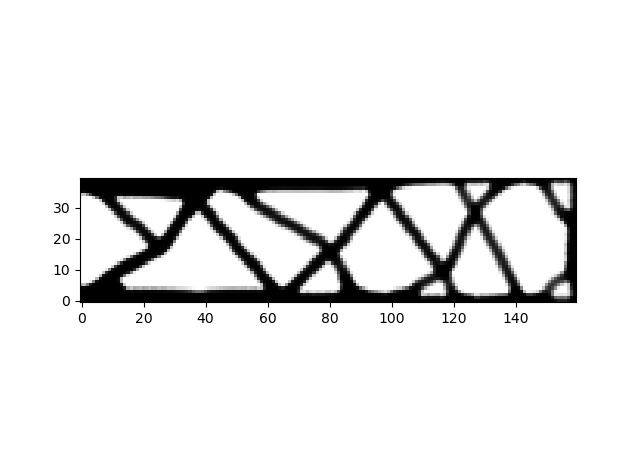
\includegraphics[width=1\textwidth]{./images/robust_approx/trace_Hadamard10_mean_csimp.png}
    \caption{Trace estimation method with 10 Hadamard basis probing vectors.}
  \end{subfigure}
  \caption{Optimal topologies of the mean compliance minimization problem using continuation SIMP.}
  \label{fig:mean}
\end{figure}

\begin{table}
 \centering
 \caption{Summary statistics of the load compliances of the optimal solution of the mean compliance minimization problem using the exact and trace estimation methods to evaluate the mean compliance. 10 Hadamard basis probing vectors were used in the trace estimator.}
 \begin{tabular}{|c|c|c|}
  %1.1 - 0.7 - 0.5
  \hline
  \multirow{2}{5em}{Compliance Stat} & \multicolumn{2}{c|}{Value} \\\cline{2-3}
  & Exact & Trace estimation \\
  \hline
  \hline
  $\mu_C$ (Nmm) & 9397.4 & 7534.1 (uncorrected approx) / 9563.4 (exact) \\
  \hline
  $\sigma_C$ (Nmm) & 9689.0 & 9698.8 \\
  \hline
  $C_{max}$ (Nmm) & 125440.7 & 124021.8 \\
  \hline
  $C_{min}$ (Nmm) & 468.7 & 380.8 \\
  \hline
  $V$ & 0.400 & 0.400 \\
  \hline
  $Time$ (s) & 25505.4 & 375.5 \\
  \hline
 \end{tabular}
 \label{tab:mean_stats}
\end{table}

\subsubsection{Mean-std compliance minimization}

Similarly, Table \ref{tab:mean_std_stats} shows the statistics of the final solutions of the mean-std minimization problem solved using the exact and the corrected diagonal estimator method with 10 Hadamard basis probing vectors. The optimal topologies are shown in Figure \ref{fig:mean_std}. Both algorithms converged to reasonable, feasible designs. Additionally, as expected the exact and approximate mean-std minimization algorithms converged to solutions with lower compliance standard deviations but higher means compared to the exact and approximate mean minimization algorithms. It should be noted that the approximation error and non-convexity of the problem can sometimes lead this expectation to be unmet with the approximate approaches. The results indicate that the approximate method is able to converge in a fraction of the time it takes the exact method to converge because evaluating the function and its gradient using diagonal estimation requires $2N = 20$ linear system solves while the naive exact method requires 1000. This problem uses a low rank $\bm{F}$. The results of using the approximate methods proposed to solve a problem with a load matrix $\bm{F}$ of rank 100 are shown in the next section.

\begin{figure}
  \begin{subfigure}[t]{0.8\textwidth}
    \centering
    \includegraphics[width=1\textwidth]{./images/robust_approx/exact_svd_mean_std_csimp.png}
    \caption{Exact method.}
  \end{subfigure} \hfill
  \begin{subfigure}[t]{0.8\textwidth}
    \centering
    \includegraphics[width=1\textwidth]{./images/robust_approx/diagonal_mean_std_csimp.png}
    \caption{Corrected diagonal estimation method with 10 Hadamard basis probing vectors using the estimator in Eq. \ref{eqn:corrected_estimator}.}
  \end{subfigure}
  \caption{Optimal topologies of the mean-std compliance minimization problem using continuation SIMP.}
  \label{fig:mean_std}
\end{figure}

\begin{table*}
 \centering
 \caption{Summary statistics of the load compliances of the optimal solution of the mean-std compliance minimization problem using exact and the corrected diagonal estimation method with 10 Hadamard basis probing vectors to evaluate the mean-std compliance.}
 \begin{tabular}{|c|c|c|}
  \hline
  \multirow{2}{5em}{Compliance Stat} & \multicolumn{2}{c|}{Value} \\\cline{2-3}
  & Exact & Diagonal estimation \\
  \hline
  \hline
  $\mu_C (Nmm) $ & 9871.6 & 9906.6 (corrected approx) / 9809.8 (exact) \\
  \hline
  $\sigma_C (Nmm) $ & 9264.0 & 9225.4 (corrected approx) / 9348.6 (exact) \\
  \hline
  $\mu_C + 2.0 \sigma_C (Nmm) $ & 28407.6 & 28357.4 (corrected approx) / 28513.4 (exact) \\
  \hline
  $C_{max}$ (Nmm) & 117956.4 & 118853.9 \\
  \hline
  $C_{min}$ (Nmm) & 530.2 & 451.9 \\
  \hline
  $V$ & 0.400 & 0.400 \\
  \hline
  Time (s) & 2821.1 & 540.0 \\
  \hline
 \end{tabular}
 \label{tab:mean_std_stats}
\end{table*}

\subsection{High rank loads}

  In this section, the 2D problems solved above will be solved using a load scenarios matrix $\bm{F}$ of rank $R = 100$ instead of 10. Additionally, the SVD-based method proposed by \cite{tarek2021robust} will be used instead of the naive approach used above. This will highlight the disadvantage of the SVD-based method when using a high rank $\bm{F}$.
  
  The results are shown to be consistent with the low rank $\bm{F}$ where the corrected estimator's accuracy is significantly improved by a single correction at the beginning of the optimization. The histograms in Figures \ref{fig:correcting_mean_high_rank} and \ref{fig:correcting_std_high_rank} also suggest that the correcting ratio is insensitive to the design. Figure \ref{fig:exact_approx_high_rank} shows that the Hadamard probing vectors do not always give a better estimator than the Rademacher-distributed one for the mean but it is consistently better for the standard deviation. Figures \ref{fig:mean_high_rank} and \ref{fig:mean_std_high_rank} and tables \ref{tab:mean_stats_high_rank} and \ref{tab:mean_std_stats_high_rank} show the optimal topologies and results obtained using the exact and approximate methods. The results are consistent with the expectations.
    \begin{figure}
      \begin{subfigure}[t]{0.45\textwidth}
        \centering
        \includegraphics[width=1\textwidth]{./images/robust_approx/results_2d_high_rank_figures/exact_approx_mean.png}
        \caption{Mean compliance estimate using different numbers of probing vectors in the trace estimation method.}
        \label{fig:exact_approx_mean_high_rank}
      \end{subfigure} \hfill
      \begin{subfigure}[t]{0.45\textwidth}
        \centering
        \includegraphics[width=1\textwidth]{./images/robust_approx/results_2d_high_rank_figures/exact_approx_std.png}
        \caption{Compliance standard deviation estimate using different numbers of probing vectors in the diagonal estimation method.}
        \label{fig:exact_approx_std_high_rank}
      \end{subfigure}
      \caption{Accuracy profile of the trace and diagonal estimation methods for estimating the mean compliance and its standard deviation using 10, 100, 200, 300, 400, 500, 600, 700, 800, 900 and 1000 probing vectors for the high rank $\bm{F}$ case.}
      \label{fig:exact_approx_high_rank}
    \end{figure}

    \begin{figure}
      \begin{subfigure}[t]{0.45\textwidth}
        \centering
        \includegraphics[width=1\textwidth]{./images/robust_approx/results_2d_high_rank_figures/correcting_factors_hadamard_mean_10_01.png}
        \caption{Mean = 0.1}
      \end{subfigure}
      \begin{subfigure}[t]{0.45\textwidth}
        \centering
        \includegraphics[width=1\textwidth]{./images/robust_approx/results_2d_high_rank_figures/correcting_factors_hadamard_mean_10_03.png}
        \caption{Mean = 0.3}
      \end{subfigure}
      \begin{subfigure}[t]{0.45\textwidth}
        \centering
        \includegraphics[width=1\textwidth]{./images/robust_approx/results_2d_high_rank_figures/correcting_factors_hadamard_mean_10_05.png}
        \caption{Mean = 0.5}
      \end{subfigure}
      \begin{subfigure}[t]{0.45\textwidth}
        \centering
        \includegraphics[width=1\textwidth]{./images/robust_approx/results_2d_high_rank_figures/correcting_factors_hadamard_mean_10_07.png}
        \caption{Mean = 0.7}
      \end{subfigure}
      \begin{subfigure}[t]{0.45\textwidth}
        \centering
        \includegraphics[width=1\textwidth]{./images/robust_approx/results_2d_high_rank_figures/correcting_factors_hadamard_mean_10_09.png}
        \caption{Mean = 0.9}
      \end{subfigure}
      \caption{Histograms of the ratio between the exact mean compliance and the trace estimate using 10 Hadamard basis probing vectors for the high rank $\bm{F}$. In each figure, 500 designs were randomly sampled where each element's pseudo-density is sampled from a truncated normal distribution with the means indicated above and a standard deviation of 0.2, truncated between 0 and 1.}
      \label{fig:correcting_mean_high_rank}
    \end{figure}
    \begin{figure}
      \begin{subfigure}[t]{0.45\textwidth}
        \centering
        \includegraphics[width=1\textwidth]{./images/robust_approx/results_2d_high_rank_figures/correcting_factors_hadamard_std_10_01.png}
        \caption{Mean = 0.1}
      \end{subfigure}
      \begin{subfigure}[t]{0.45\textwidth}
        \centering
        \includegraphics[width=1\textwidth]{./images/robust_approx/results_2d_high_rank_figures/correcting_factors_hadamard_std_10_03.png}
        \caption{Mean = 0.3}
      \end{subfigure}
      \begin{subfigure}[t]{0.45\textwidth}
        \centering
        \includegraphics[width=1\textwidth]{./images/robust_approx/results_2d_high_rank_figures/correcting_factors_hadamard_std_10_05.png}
        \caption{Mean = 0.5}
      \end{subfigure}
      \begin{subfigure}[t]{0.45\textwidth}
        \centering
        \includegraphics[width=1\textwidth]{./images/robust_approx/results_2d_high_rank_figures/correcting_factors_hadamard_std_10_07.png}
        \caption{Mean = 0.7}
      \end{subfigure}
      \begin{subfigure}[t]{0.45\textwidth}
        \centering
        \includegraphics[width=1\textwidth]{./images/robust_approx/results_2d_high_rank_figures/correcting_factors_hadamard_std_10_09.png}
        \caption{Mean = 0.9}
      \end{subfigure}
      \caption{Histograms of the ratio between the exact compliance standard deviation and the estimate using 10 Hadamard basis probing vectors for the high rank $\bm{F}$ case. In each figure, 500 designs were randomly sampled where each element's pseudo-density is sampled from a truncated normal distribution with the means indicated above and a standard deviation of 0.2, truncated between 0 and 1.}
      \label{fig:correcting_std_high_rank}
    \end{figure}

    \begin{figure}
      \begin{subfigure}[t]{0.9\textwidth}
        \centering
        \includegraphics[width=1\textwidth]{./images/robust_approx/results_2d_high_rank_figures/exact_svd_mean_csimp.png}
        \caption{Exact method.}
      \end{subfigure} \hfill
      \begin{subfigure}[t]{0.8\textwidth}
        \centering
        \includegraphics[width=1\textwidth]{./images/robust_approx/results_2d_high_rank_figures/trace_Hadamard10_mean_csimp.png}
        \caption{Trace estimation method with 10 Hadamard basis probing vectors.}
      \end{subfigure}
      \caption{Optimal topologies of the mean compliance minimization problem with a high rank $\bm{F}$ using continuation SIMP.}
      \label{fig:mean_high_rank}
    \end{figure}

    \begin{table}
     \centering
     \caption{Summary statistics of the load compliances of the optimal solution of the mean compliance minimization problem with a high rank $\bm{F}$ using the exact and trace estimation methods to evaluate the mean compliance. 10 Hadamard basis probing vectors were used in the trace estimator.}
     \begin{tabular}{|c|c|c|}
      %1.1 - 0.7 - 0.5
      \hline
      \multirow{2}{5em}{Compliance Stat} & \multicolumn{2}{c|}{Value} \\\cline{2-3}
      & Exact & Trace estimation \\
      \hline
      \hline
      $\mu_C$ (Nmm) & 2084.3 & 1094.1 (uncorrected approx) / 2226.4 (exact) \\
      \hline
      $\sigma_C$ (Nmm) & 2226.6 & 2412.0 \\
      \hline
      $C_{max}$ (Nmm) & 15971.9 & 16793.3 \\
      \hline
      $C_{min}$ (Nmm) & 171.0 & 152.0 \\
      \hline
      $V$ & 0.400 & 0.400 \\
      \hline
      $Time$ (s) & 2123.0 & 485.3 \\
      \hline
     \end{tabular}
     \label{tab:mean_stats_high_rank}
    \end{table}

    \begin{figure}
      \begin{subfigure}[t]{0.8\textwidth}
        \centering
        \includegraphics[width=1\textwidth]{./images/robust_approx/results_2d_high_rank_figures/exact_svd_mean_std_csimp.png}
        \caption{Exact method.}
      \end{subfigure} \hfill
      \begin{subfigure}[t]{0.8\textwidth}
        \centering
        \includegraphics[width=1\textwidth]{./images/robust_approx/results_2d_high_rank_figures/diagonal_mean_std_csimp.png}
        \caption{Corrected diagonal estimation method with 10 Hadamard basis probing vectors using the estimator in Eq. \ref{eqn:corrected_estimator}.}
      \end{subfigure}
      \caption{Optimal topologies of the mean-std compliance minimization problem with high rank $\bm{F}$ using continuation SIMP.}
      \label{fig:mean_std_high_rank}
    \end{figure}

    \begin{table}
     \centering
     \caption{Summary statistics of the load compliances of the optimal solution of the mean-std compliance minimization problem with a high rank $\bm{F}$ using exact and the corrected diagonal estimation method with 10 Hadamard basis probing vectors to evaluate the mean-std compliance.}
     \begin{tabular}{|c|c|c|}
      \hline
      \multirow{2}{5em}{Compliance Stat} & \multicolumn{2}{c|}{Value} \\\cline{2-3}
      & Exact & Diagonal estimation \\
      \hline
      \hline
      $\mu_C$ (Nmm) & 2151.9 & 2336.8 (corrected approx) / 2147.5 (exact) \\
      \hline
      $\sigma_C$ (Nmm) & 2149.0 & 2195.7 (corrected approx) / 2234.2 (exact) \\
      \hline
      $\mu_C + 2.0 \sigma_C$ (Nmm) & 6450.6 & 6728.3 (corrected approx) / 6616.7 (exact) \\
      \hline
      $C_{max}$ (Nmm) & 15558.2 & 15559.4 \\
      \hline
      $C_{min}$ (Nmm) & 187.4 & 161.6 \\
      \hline
      $V$ & 0.400 & 0.400 \\
      \hline
      Time (s) & 6435.4 & 650.1 \\
      \hline
     \end{tabular}
     \label{tab:mean_std_stats_high_rank}
    \end{table}

    As shown in tables \ref{tab:mean_stats_high_rank} and \ref{tab:mean_std_stats_high_rank}, the SVD-based methods are slower than the approximation schemes proposed when the rank of the loads is high. This is because the number of non-zero singular values will be 100 which is 10x the number of probing vectors used. In the mean compliance minimization, a 10 speedup is achieved which is consistent with the expectation. In the mean-std compliance minimization, the diagonal estimation method requires 20 linear system solves so only a factor of 5 speedup is achieved with the approximate method compared to the SVD-based method.
    
\subsection{3D cantilever beam problem}

  A 3D version of the 2D cantilever beam test problem used above was also solved using the methods proposed in this chapter. The problem settings are described and the results are shown below.

  A 60 mm x 20 mm x 20 mm 3D cantilever beam was used with hexahedral elements of cubic shape and side length of 1 mm. The loads $\bm{F}_1$, $\bm{F}_2$ and $\bm{F}_3$ were positioned at (60, 10, 10), (30, 20, 10) and (40, 0, 10) where the coordinates represent the length, height and depth respectively. A value of $R = 10$ was used. The remaining loads and multipliers were sampled from the same distributions as the 2D problem. A density filter radius of 3 mm was also used for the 3D problem. The same volume constrained mean compliance minimization and volume constrained mean-std compliance minimization problems were solved.

  \subsubsection{Mean compliance minimization}

    \begin{figure}
      \begin{subfigure}[t]{0.45\textwidth}
        \centering
        \includegraphics[width=1\textwidth]{./images/robust_approx/exact_mean_1.png}
        \caption{Left half}
      \end{subfigure} \hfill
      \begin{subfigure}[t]{0.45\textwidth}
        \centering
        \includegraphics[width=1\textwidth]{./images/robust_approx/exact_mean_2.png}
        \caption{Right half}
      \end{subfigure}
      \caption{Cut views of the optimal topologies of the 3D mean compliance minimization problem using exact method.}
      \label{fig:exact_mean_3d}
    \end{figure}

    \begin{figure}
      \begin{subfigure}[t]{0.45\textwidth}
        \centering
        \includegraphics[width=1\textwidth]{./images/robust_approx/trace_mean_1.png}
        \caption{Left half}
      \end{subfigure} \hfill
      \begin{subfigure}[t]{0.45\textwidth}
        \centering
        \includegraphics[width=1\textwidth]{./images/robust_approx/trace_mean_2.png}
        \caption{Right half}
      \end{subfigure}
      \caption{Cut views of the optimal topologies of the 3D mean compliance minimization problem using the trace estimation method.}
      \label{fig:trace_mean_3d}
    \end{figure}

    \begin{table}
     \centering
     \caption{Summary statistics of the load compliances of the optimal solution of the 3D mean compliance minimization problem using the exact and trace estimation methods to evaluate the mean compliance. 10 Hadamard basis probing vectors were used in the trace estimator.}
     \begin{tabular}{|c|c|c|}
      %1.1 - 0.7 - 0.5
      \hline
      \multirow{2}{5em}{Compliance Stat} & \multicolumn{2}{c|}{Value} \\\cline{2-3}
      & Exact & Trace estimation \\
      \hline
      \hline
      $\mu_C$ (Nmm) & 22072.1 & 24710.5 (uncorrected approx) / 22264.3 (exact) \\
      \hline
      $\sigma_C$ (Nmm) & 16628.7 & 17055.2 \\
      \hline
      $C_{max}$ (Nmm) & 184055.0 & 190599.9 \\
      \hline
      $C_{min}$ (Nmm) & 1785.8 & 1790.9 \\
      \hline
      $V$ & 0.400 & 0.400 \\
      \hline
      $Time$ (s) & 167321.2 & 6595.2 \\
      \hline
     \end{tabular}
     \label{tab:mean_stats_3d}
    \end{table}

    The 3D cantilever beam problem described above was solved using the proposed approximate methods with the objective of minimizing the mean compliance subject to a volume fraction constraint with a limit of 0.4. Table \ref{tab:mean_stats_3d} shows the statistics of the final optimal solutions obtained by minimizing the mean compliance subject to the volume fraction constraint using the naive exact approach and the trace estimation method to evaluate the mean compliance. 10 Hadamard basis probing vectors were used in the trace estimator. The optimal topologies are shown in Figures \ref{fig:exact_mean_3d} and \ref{fig:trace_mean_3d}. Similar results to the 2D case can be observed where the designs obtained are different but somewhat reasonable. The proposed method converged in a small fraction of the time that the naive method took to converge. However, the design produced by the trace estimation method was worse than the exact method's which is to be expected since an approximate objective was minimized. Finally, note that the corrected estimate is close to the exact value.

  \subsubsection{Mean-std compliance minimization}

    \begin{figure}
      \begin{subfigure}[t]{0.45\textwidth}
        \centering
        \includegraphics[width=1\textwidth]{./images/robust_approx/exact_mean_std_1.png}
        \caption{Left half}
      \end{subfigure} \hfill
      \begin{subfigure}[t]{0.45\textwidth}
        \centering
        \includegraphics[width=1\textwidth]{./images/robust_approx/exact_mean_std_2.png}
        \caption{Right half}
      \end{subfigure}
      \caption{Cut views of the optimal topologies of the 3D mean-std compliance minimization problem using the exact method.}
      \label{fig:exact_mean_std_3d}
    \end{figure}

    \begin{figure}
      \begin{subfigure}[t]{0.45\textwidth}
        \centering
        \includegraphics[width=1\textwidth]{./images/robust_approx/diagonal_mean_std_1.png}
        \caption{Left half}
      \end{subfigure} \hfill
      \begin{subfigure}[t]{0.45\textwidth}
        \centering
        \includegraphics[width=1\textwidth]{./images/robust_approx/diagonal_mean_std_2.png}
        \caption{Right half}
      \end{subfigure}
      \caption{Cut views of the optimal topologies of the 3D mean-std compliance minimization problem using the corrected diagonal estimation method.}
      \label{fig:diagonal_mean_std_3d}
    \end{figure}

    \begin{table}
     \centering
     \caption{Summary statistics of the load compliances of the optimal solution of the mean-std compliance minimization problem using exact and the corrected diagonal estimation method with 10 Hadamard basis probing vectors to evaluate the mean-std compliance.}
     \begin{tabular}{|c|c|c|}
      \hline
      \multirow{2}{5em}{Compliance Stat} & \multicolumn{2}{c|}{Value} \\\cline{2-3}
      & Exact & Diagonal estimation \\
      \hline
      \hline
      $\mu_C$ (Nmm) & 22216.7 & 2240.8 (corrected approx) / 22145.9 (exact) \\
      \hline
      $\sigma_C$ (Nmm) & 16220.2 & 16501.4 (corrected approx) / 16510.0 (exact) \\
      \hline
      $\mu_C + 2.0 \sigma_C$ (Nmm) & 54848.8 & 55423.7 (corrected approx) / 55366.0 (exact) \\
      \hline
      $C_{max}$ (Nmm) & 176153.2 & 182209.8 \\
      \hline
      $C_{min}$ (Nmm) & 1872.0 & 1850.4 \\
      \hline
      $V$ & 0.400 & 0.400 \\
      \hline
      Time (s) & 39935.4 & 10949.3 \\
      \hline
     \end{tabular}
     \label{tab:mean_std_stats_3d}
    \end{table}

    Similarly, Table \ref{tab:mean_std_stats_3d} shows the statistics of the final solutions of the 3D mean-std minimization problem solved using the naive exact approach and the corrected diagonal estimator method with 10 Hadamard basis probing vectors. The optimal topologies are shown in Figures \ref{fig:exact_mean_std_3d} and \ref{fig:diagonal_mean_std_3d}. Both algorithms converged to reasonable and feasible designs. Additionally, as expected the exact mean-std minimization converged to a solution with a lower standard deviation but a higher mean compliance compared to the exact mean minimization. However, due to the approximation error and non-convexity of the problems, the exact and approximate mean-std algorithms converged to solutions with a lower mean and std compared to the approximate mean algorithm. Finally as expected, the exact method took significantly longer to converge than the diagonal estimation method.

\section{Conclusion} \label{sec:conclusion}

  In this chapter, two approximate methods were proposed to handle load uncertainty in compliance topology optimization problems where the uncertainty is described in the form of a set of finitely many loading scenarios. By re-formulating the function as a trace or diagonal estimation problem, significant performance improvements were achieved over the exact methods. Such improvement was demonstrated via complexity analysis and computational experiments. The methods proposed were shown to work well in practice while having a different time complexity profile.

	\let\cleardoublepage\clearpage
	\chapter{Conclusion and future work}\thispagestyle{EmptyHeader}
\label{chp:5}

In this thesis, a few things were achieved. Firstly, a reasonably comprehensive introduction to linear elasticity theory for topology optimization was presented. Special care was given to all the details to enable a 1-to-1 mapping from the text to the implementation. This is important when developing topology optimization codes and algorithms on unstructured meshes which is what the author here did. This was followed by a presentation of the most common topology optimization algorithms and a detailed presentation of the most common nonlinear programming algorithms used in topology optimization. The author here could not find any single reference that compiles detailed explanations of the theory behind the commonly used nonlinear programming algorithms in topology optimization, together with all their assumptions, strengths and weaknesses and tips on when to use each algorithm. Additionally, a description of all the common paradigms for decision-making under uncertainty was presented.

Realizing the importance and prevalence of CSIMP in topology optimization, all the ways to adapt the penalty step in CSIMP found in literature were reviewed. A gap was found for a general penalty adaptation technique for CSIMP. A flexible and theoretically sound way to adapt penalties was proposed which gave significant speedups in the experiments run. Four common test problems from literature, three 2D and one 3D, were used to test the efficacy of the penalty adaptation with different parameter settings. The main factors affecting the efficacy of the penalty adaptation in the CSIMP algorithm in reducing the number of FEA simulations needed to converge to the final solution were identified. The experimental results demonstrate a significant reduction in the number of FEA simulations required to reach the optimal solution in the decreasing tolerance continuation SIMP algorithm, with exponentially decaying tolerance, with little to no detriment in the objective value and the other metrics used. Finally, a mathematical and experimental treatment of the effect of $x_{min}$ on the convergence of the SIMP algorithm was given with some recommendations for choosing a suitable $x_{min}$. These results were published in \cite{TAREK2020112880}. Some potential future work here is to perform more experiments on more problem classes as well as a larger benchmark set involving more problem classes. To this day, there is a lack of a standard benchmark set for topology optimization across algorithms and programming languages. Preparing such data set will be extremely valuable to the topology optimization society.

Handling load uncertainty significantly increases the computational cost of any algorithm. A comprehensive review of all the literature on handling uncertainty in compliance-based problems was therefore conducted and presented. And a number of exact methods were proposed to handle load uncertainty in compliance-based topology optimization problems where the uncertainty is described in the form of a set of finitely many loading scenarios. This includes mean compliance minimization or a constraint on the mean compliance, minimizing or constraining a weighted sum of the mean and standard deviation of the load compliances as well as minimizing or constraining the maximum load compliance for all the loading scenarios. By detecting and exploiting low rank structures in the loading scenarios, significant performance improvements were achieved using some novel SVD-based methods. The computational complexities of the algorithms proposed were demonstrated and experiments were run to verify the efficacy of the proposed algorithms at reducing the computational cost of these classes of topology optimization problems. The methods presented here are fundamentally data-driven in the sense that no probability distributions or domains are assumed for the loading scenarios. This sets this work apart from most of the literature in the domain of stochastic and robust topology optimization where a distribution or domain is assumed. Additionally, the methods proposed here were shown to be particularly suitable with the augmented Lagrangian algorithm when dealing with maximum compliance constraints. This work was accepted for publication the Structural and Multidisciplinary Optimization journal. Some potential future work here includes developing algorithms for data-driven topology optimization under uncertainty for other classes of topology optimization problems.

Given that the exact methods for handling many loading scenarios require that a low rank exists, more efficient methods were developed when no such low rank exists. In particular, approximation schemes for the mean compliance and a class of scalar-valued functions of the load compliances were developed. The approximation schemes were based on a reformulation of the function approximated as a trace or diagonal estimation problem, opening the door to using many of the available methods for trace or diagonal estimation. The approximation methods were tested on a number of standard 2D and 3D benchmark problems using low and high rank loading scenarios to solve mean compliance minimization as well as minimizing the weighted sum of the mean compliance and its standard deviation. Significant speedups were achieved compared to the naive method as well as the SVD-based method when the rank of the load matrix is high. This work was submitted to the Structural and Multidisciplinary Optimization journal as of the time of writing this thesis. There are a number of possible extensions to this work including trying or developing other trace and diagonal estimators. More generally, developing approximation schemes for other classes of topology optimization problems where there are finitely many loading scenarios is a largely untouched area of research.

Beside the potential future directions suggested above, there are many other potential future works in topology optimization. In particular, one promising direction to purse is the use of differentiable programming and automatic differentiation for topology optimization to simplify and generalize implementations of topology optimization algorithms in multi-physics applications. This is a direction the author is currently pursuing.

	\let\cleardoublepage\clearpage
	
	%\rhead{BIBLIOGRAPHY}
%	\chapter*{REFERENCES}
	\thispagestyle{EmptyHeader}
	\label{biblio}
	
	\bibliography{References/refFile}
	\bibliographystyle{agsm}
	
	\let\cleardoublepage\clearpage
	\appendix
\addappheadtotoc
%\chapter{Appendices}
\setcounter{table}{0}
\renewcommand{\thetable}{A\arabic{table}}

\setcounter{figure}{0}
\renewcommand{\thefigure}{B\arabic{figure}}

\section{Partial derivative of the inverse quadratic form} \label{app1}

In this section, it will be shown that the $i^{th}$ partial derivative of:
\begin{align}
  f(\bm{x}) & = \bm{v}^T (\bm{A}(\bm{x}))^{-1} \bm{v}
\end{align}
is
\begin{align}
  \frac{\partial f}{\partial x_i} & = -\bm{y}^T \frac{\partial \bm{A}}{\partial x_i} \bm{y}^T
\end{align}
where $\bm{A}$ is a matrix-valued function of $\bm{x}$, $\bm{v}$ is a constant vector and $\bm{y} = \bm{A}^{-1} \bm{v}$ is a an implicit function of $\bm{x}$ because $\bm{A}$ is a function of $\bm{x}$.

\begin{align}
  \bm{v} & = \bm{A} \bm{y} \\
  \bm{0} & = \bm{A} \frac{\partial \bm{y}}{\partial x_i} + \frac{\partial \bm{A}}{\partial x_i} \bm{y} \\
  \frac{\partial y}{\partial x_i} & = - \bm{A}^{-1} \frac{\partial \bm{A}}{\partial x_i} \bm{y} \\
  f(\bm{x}) & = \bm{v}^T \bm{A}^{-1} \bm{v} \\
  & = \bm{y}^T \bm{A} \bm{y} \\
  \frac{\partial f}{\partial x_i} & = 2 \bm{y}^T \bm{A} \frac{\partial \bm{y}}{\partial x_i} + \bm{y}^T \frac{\partial \bm{A}}{\partial x_i} \bm{y} \\
  & = - 2 \bm{y}^T \bm{A} \bm{A}^{-1} \frac{\partial \bm{A}}{\partial x_i} \bm{y} + \bm{y}^T \frac{\partial \bm{A}}{\partial x_i} \bm{y} \\
  & = - 2 \bm{y}^T \frac{\partial \bm{A}}{\partial x_i} \bm{y} + \bm{y}^T \frac{\partial \bm{A}}{\partial x_i} \bm{y} \\
  & = - \bm{y}^T \frac{\partial \bm{A}}{\partial x_i} \bm{y}
\end{align}

	
%	\let\cleardoublepage\clearpage
%	\rhead{\leftmark}
%	\let\cleardoublepage\clearpage
%	\include{StudyPlan/plan}
\end{document}
